\documentclass[12pt,a4paper,oneside]{report}

% =========================================================================
% CẤU HÌNH THÔNG TIN TRANG BÌA (CHỈ CẦN SỬA TẠI ĐÂY)
% =========================================================================
\newcommand{\TenTruong}{TRƯỜNG ĐẠI HỌC [ĐIỀN TÊN TRƯỜNG]}
\newcommand{\TenKhoa}{KHOA CÔNG NGHỆ THÔNG TIN}
\newcommand{\TenMonHoc}{PHÂN TÍCH VÀ THIẾT KẾ HỆ THỐNG THÔNG TIN}
\newcommand{\TenDeTai}{PHÂN TÍCH, THIẾT KẾ VÀ XÂY DỰNG HỆ THỐNG\\QUẢN LÝ BÁN VÉ XEM PHIM LUMICINEMA}
\newcommand{\GiangVienHD}{[ĐIỀN TÊN GIẢNG VIÊN HƯỚNG DẪN]}
\newcommand{\MaLop}{[ĐIỀN MÃ LỚP]}
\newcommand{\TenNhom}{Nhóm 10}
\newcommand{\NamHoc}{TP. Hồ Chí Minh, năm 2026}

% Danh sách 5 thành viên (sửa MSSV tại đây)
\newcommand{\TVMot}{Mã Gia Vỹ & [MSSV 1] & Nhóm trưởng, Sơ đồ tổng quát, Kiến trúc}
\newcommand{\TVHai}{Nguyễn Khánh Hưng & [MSSV 2] & Mua vé \& Combo online, Quản trị danh mục}
\newcommand{\TVBa}{Nguyễn Hữu Thắng & [MSSV 3] & Hủy vé \& Bồi hoàn, Báo cáo doanh thu}
\newcommand{\TVBon}{Hoàng Gia Bảo & [MSSV 4] & Bán vé \& Soát vé tại quầy (POS)}
\newcommand{\TVNam}{Quốc Việt & [MSSV 5] & Đánh giá phim, Quản lý vé khách hàng}

% =========================================================================
% GÓI THƯ VIỆN CHUẨN XELATEX + TIẾNG VIỆT (CHẠY MƯỢT TRÊN OVERLEAF)
% =========================================================================
\usepackage{fontspec}
\setmainfont{TeX Gyre Termes} % Font giống Times New Roman, có sẵn 100% trên Overleaf
\setsansfont{TeX Gyre Heros}
\setmonofont[Scale=0.85]{DejaVu Sans Mono}

\usepackage{polyglossia}
\setdefaultlanguage{vietnamese}

\usepackage[top=2.5cm,bottom=2.5cm,left=3.0cm,right=2.0cm]{geometry}
\usepackage{graphicx}
\usepackage{float}
\usepackage{longtable}
\usepackage{array}
\usepackage{booktabs}
\usepackage{multirow}
\usepackage[table]{xcolor}
\usepackage{hyperref}
\usepackage{titlesec}
\usepackage{fancyhdr}
\usepackage{setspace}
\usepackage{caption}
\usepackage{tikz}
\usepackage{enumitem}

\definecolor{headerblue}{RGB}{224,235,248}
\definecolor{accentred}{RGB}{185,28,28}
\definecolor{bordergray}{RGB}{148,163,184}

\hypersetup{
    colorlinks=true,
    linkcolor=black,
    urlcolor=blue,
    citecolor=black,
    pdftitle={Báo cáo đồ án LumiCinema - Nhóm 10},
    pdfauthor={Nhóm 10}
}

\onehalfspacing
\setlength{\parindent}{0.7cm}
\setlength{\parskip}{4pt}

% Header & Footer
\pagestyle{fancy}
\fancyhf{}
\fancyhead[L]{\small\textit{Đồ án Phân tích \& Thiết kế Hệ thống --- LumiCinema}}
\fancyhead[R]{\small\textit{\TenNhom}}
\fancyfoot[C]{\thepage}
\renewcommand{\headrulewidth}{0.4pt}

% Tiêu đề chương tiếng Việt
\titleformat{\chapter}[display]
  {\normalfont\huge\bfseries\centering}
  {CHƯƠNG \thechapter}{10pt}{\LARGE}
\titlespacing*{\chapter}{0pt}{-20pt}{20pt}

\begin{document}

% =========================================================================
% TRANG BÌA
% =========================================================================
\begin{titlepage}
\begin{tikzpicture}[remember picture, overlay]
  \draw[line width=2pt] ([xshift=1.5cm,yshift=-1.5cm]current page.north west) rectangle ([xshift=-1.5cm,yshift=1.5cm]current page.south east);
  \draw[line width=0.6pt] ([xshift=1.7cm,yshift=-1.7cm]current page.north west) rectangle ([xshift=-1.7cm,yshift=1.7cm]current page.south east);
\end{tikzpicture}

\centering
\vspace*{0.5cm}
{\large\bfseries \TenTruong \par}
{\large\bfseries \TenKhoa \par}
\vspace{1.2cm}

{\Large\bfseries BÁO CÁO ĐỒ ÁN MÔN HỌC \par}
\vspace{0.3cm}
{\large\bfseries \TenMonHoc \par}
\vspace{1.5cm}

\rule{\linewidth}{0.8pt}\\[0.4cm]
{\LARGE\bfseries \TenDeTai \par}
\vspace{0.2cm}
\rule{\linewidth}{0.8pt}

\vspace{1.8cm}
\begin{flushleft}
\hspace{1.2cm}\textbf{Giảng viên hướng dẫn:} \GiangVienHD \\[0.3cm]
\hspace{1.2cm}\textbf{Lớp:} \MaLop \hfill \textbf{Nhóm thực hiện:} \TenNhom \hspace{1.2cm}
\end{flushleft}

\vspace{0.6cm}
\begin{center}
\renewcommand{\arraystretch}{1.35}
\begin{tabular}{|p{4.5cm}|p{2.6cm}|p{6.8cm}|}
\hline
\rowcolor{headerblue} \textbf{Họ và tên} & \textbf{MSSV} & \textbf{Phụ trách chính} \\ \hline
\TVMot \\ \hline
\TVHai \\ \hline
\TVBa \\ \hline
\TVBon \\ \hline
\TVNam \\ \hline
\end{tabular}
\end{center}

\vfill
{\large\bfseries \NamHoc \par}
\vspace*{0.5cm}
\end{titlepage}

% =========================================================================
% MỤC LỤC, DANH MỤC HÌNH ẢNH, DANH MỤC BẢNG BIỂU
% =========================================================================
\pagenumbering{roman}
\tableofcontents
\clearpage
\listoffigures
\clearpage
\listoftables
\clearpage

% =========================================================================
% NỘI DUNG CHÍNH
% =========================================================================
\pagenumbering{arabic}

\chapter{GIỚI THIỆU ĐỀ TÀI}
\section{Bối cảnh và Lý do chọn đề tài}
Một nhóm sinh viên muốn khởi nghiệp (startup) xây dựng một rạp chiếu phim quy mô nhỏ mang thương hiệu \textbf{LumiCinema}, nhằm phục vụ khách hàng xem phim và đặt vé linh hoạt theo hai hình thức: \textbf{đặt vé trực tuyến (Online)} và \textbf{mua vé trực tiếp tại quầy (POS)}. Bên cạnh dịch vụ bán vé, rạp còn kinh doanh các gói bắp nước (Combo) nhằm gia tăng trải nghiệm và tối ưu doanh thu.

Để vận hành đồng bộ, minh bạch, tránh sai sót trong khâu giữ ghế, thanh toán, đối soát doanh thu và xử lý sự cố (hủy vé, hoàn tiền, cấp voucher bồi hoàn), việc phân tích, thiết kế và xây dựng một hệ thống quản lý bán vé xem phim hoàn chỉnh là yêu cầu cấp thiết.

\section{Phạm vi hệ thống}
Hệ thống LumiCinema được thiết kế cho \textbf{một rạp chiếu phim duy nhất} với các thông số vận hành chuẩn hóa như sau:
\begin{itemize}[leftmargin=1.2cm]
  \item \textbf{Quy mô phòng chiếu:} Gồm \textbf{5 phòng chiếu}, mỗi phòng có \textbf{50 ghế cùng loại} (tổng cộng \textbf{250 ghế}).
  \item \textbf{Cấu trúc sơ đồ ghế:} Mỗi phòng 50 ghế được đánh số cố định gồm 5 hàng dọc từ \textbf{A đến E} và 10 cột ngang từ \textbf{1 đến 10} (A1--A10, ..., E1--E10).
  \item \textbf{Kênh bán vé:} Hỗ trợ đồng thời \textbf{2 kênh} là Online (qua web, thanh toán qua cổng ZaloPay/VNPay có số dư và nạp tiền) và Tại quầy (POS tiền mặt/chuyển khoản).
  \item \textbf{Thông báo tự động:} Gửi email xác nhận đặt vé, email cấp voucher bồi hoàn và email xác nhận hoàn tiền mặt qua giao thức SMTP (Nodemailer).
\end{itemize}

\section{Mục tiêu của đồ án}
\begin{enumerate}[leftmargin=1.2cm]
  \item Phân tích đầy đủ yêu cầu nghiệp vụ, lập mô hình BFD, Use Case, Sequence, Activity, State, Class và thiết kế CSDL (ERD/RDM) nhất quán 100\% với mã nguồn.
  \item Xây dựng ứng dụng web hoàn chỉnh đáp ứng đầy đủ quy trình nghiệp vụ của 3 nhóm người dùng: \textbf{Khách hàng}, \textbf{Nhân viên quầy} và \textbf{Admin}.
  \item Đảm bảo tính toàn vẹn dữ liệu trong các bài toán đồng thời (giữ ghế có thời hạn TTL, chống đặt trùng ghế, cập nhật tồn kho combo, đối soát giao dịch thanh toán và hoàn tiền).
\end{enumerate}

\section{Nhóm người dùng và các chức năng chính}
\begin{table}[H]
\centering
\caption{Phân nhóm người dùng và các chức năng chính của LumiCinema}
\label{tab:actors_functions}
\renewcommand{\arraystretch}{1.3}
\begin{tabular}{|p{3.0cm}|p{12.2cm}|}
\hline
\rowcolor{headerblue} \textbf{Nhóm người dùng} & \textbf{Chức năng chính} \\ \hline
\textbf{Khách hàng} & Đăng ký, đăng nhập, xem danh sách phim và suất chiếu, chọn ghế và loại vé, đặt combo bắp nước, áp dụng voucher, thanh toán online (ZaloPay/VNPay Gateway), xem lịch sử vé, yêu cầu hủy vé trước $\ge$ 2 giờ (nhận voucher 50\%), đánh giá phim (1--5 sao và bình luận). \\ \hline
\textbf{Nhân viên quầy} & Bán vé và combo tại quầy (POS), tìm/gắn khách hàng theo SĐT/Email, áp dụng voucher, soát vé bằng mã vé/QR để cho phép vào rạp, giao combo (cập nhật trạng thái đã nhận), hỗ trợ hủy vé theo yêu cầu khách (voucher 50\%) và xử lý hủy vé sự cố rạp 1 bước (hoàn 100\% tiền mặt hoặc voucher 100\%). \\ \hline
\textbf{Admin} & Quản lý danh mục Phim (thêm, sửa, ngừng chiếu), Suất chiếu (thêm, sửa, tự động khởi tạo 50 ghế, hủy suất chiếu sự cố), Combo (thêm, sửa, ngừng bán, cập nhật tồn kho), Voucher (thêm, sửa, ngừng sử dụng), xem Dashboard doanh thu trực quan (Streamgraph) và xuất báo cáo CSV. \\ \hline
\end{tabular}
\end{table}


\chapter{PHÂN TÍCH VÀ THIẾT KẾ HỆ THỐNG}
\section{Mô hình phân rã chức năng (BFD) và Kế hoạch thực hiện đồ án}

\subsection{Bảng phân rã chức năng nghiệp vụ (BFD)}
Hệ thống quản lý bán vé xem phim LumiCinema được phân rã thành 6 nhóm chức năng cấp 1 và các chức năng chi tiết cấp 2 như Bảng~\ref{tab:bfd}.

\begin{longtable}{|p{1.2cm}|p{4.3cm}|p{9.8cm}|}
\caption{Bảng phân rã chức năng nghiệp vụ (BFD) hệ thống LumiCinema} \label{tab:bfd} \\
\hline
\rowcolor{headerblue} \textbf{Mã} & \textbf{Chức năng cấp 1} & \textbf{Chức năng cấp 2} \\ \hline
\endhead
\textbf{1.0} & Quản lý tài khoản \& Xác thực & 1.1 Đăng ký tài khoản; 1.2 Đăng nhập / Đăng xuất; 1.3 Phân quyền theo vai trò (Khách hàng, Nhân viên, Admin). \\ \hline
\textbf{2.0} & Đặt vé \& Combo trực tuyến & 2.1 Xem danh sách phim \& suất chiếu; 2.2 Chọn ghế (sơ đồ 50 ghế A1--E10) \& loại vé; 2.3 Chọn combo bắp nước; 2.4 Áp dụng mã voucher; 2.5 Thanh toán qua ZaloPay/VNPay Gateway (kiểm tra số dư, nạp tiền, hoàn tiền tự động); 2.6 Gửi email xác nhận vé. \\ \hline
\textbf{3.0} & Quản lý vé khách hàng \& Đánh giá & 3.1 Xem danh sách vé đã mua; 3.2 Yêu cầu hủy vé ($\ge$ 2 giờ trước suất chiếu, nhận voucher 50\%); 3.3 Đánh giá phim (1--5 sao + bình luận). \\ \hline
\textbf{4.0} & Bán vé \& Soát vé tại quầy (POS) & 4.1 Bán vé \& combo tại quầy; 4.2 Tìm/gắn khách hàng theo SĐT/Email; 4.3 Thu tiền \& in vé; 4.4 Soát vé hợp lệ cho vào rạp; 4.5 Giao combo (chuyển trạng thái đã nhận). \\ \hline
\textbf{5.0} & Hủy vé, Bồi hoàn \& Xử lý sự cố & 5.1 Tra cứu thông tin vé tại quầy; 5.2 Hủy vé do khách (voucher 50\%); 5.3 Ép hủy vé sự cố rạp 1 bước (hoàn 100\% tiền mặt hoặc cấp voucher 100\% + gửi email); 5.4 Hủy toàn bộ suất chiếu sự cố \& giải phóng ghế. \\ \hline
\textbf{6.0} & Quản trị danh mục \& Báo cáo & 6.1 Quản lý Phim; 6.2 Quản lý Suất chiếu (khởi tạo 50 ghế); 6.3 Quản lý Combo \& tồn kho; 6.4 Quản lý Voucher; 6.5 Dashboard doanh thu (Streamgraph) \& Xuất báo cáo CSV. \\ \hline
\end{longtable}

\begin{figure}[H]
\centering
\fbox{\parbox[c][5.2cm][c]{0.92\textwidth}{\centering
\textbf{[KHUNG CHÈN ẢNH SƠ ĐỒ PHÂN RÃ CHỨC NĂNG (BFD)]}\\[6pt]
\textit{Nhóm tự chèn file ảnh BFD vào thư mục \texttt{images/} và thay dòng này bằng \texttt{\textbackslash includegraphics}.}
}}
\caption{Sơ đồ phân rã chức năng (BFD) hệ thống LumiCinema (Placeholder)}
\label{fig:bfd_placeholder}
\end{figure}

\subsection{Kế hoạch thực hiện đồ án}
Đồ án được thực hiện trong 10 tuần với sự phân công rõ ràng cho 5 thành viên trong Nhóm 10 như Bảng~\ref{tab:plan}.

\begin{table}[H]
\centering
\caption{Kế hoạch thực hiện và phân công công việc Nhóm 10}
\label{tab:plan}
\renewcommand{\arraystretch}{1.25}
\begin{tabular}{|p{1.8cm}|p{5.5cm}|p{4.3cm}|p{3.5cm}|}
\hline
\rowcolor{headerblue} \textbf{Giai đoạn} & \textbf{Nội dung công việc} & \textbf{Phụ trách chính} & \textbf{Sản phẩm đầu ra} \\ \hline
Tuần 1--2 & Khảo sát yêu cầu, lập SRS, BFD, Use Case tổng quát và đặc tả Use Case & Mã Gia Vỹ \& cả nhóm & Tài liệu SRS, Sơ đồ Use Case \\ \hline
Tuần 3--4 & Thiết kế Sequence, Activity, State, Class Diagram, ERD và RDM & Hưng, Thắng, Bảo, Việt, Vỹ & Bộ sơ đồ UML \& CSDL chuẩn \\ \hline
Tuần 5--6 & Khởi tạo Next.js + Prisma + PostgreSQL, xây dựng xác thực, đặt vé online, POS & Hưng, Bảo, Vỹ & Module Auth, Booking, POS \\ \hline
Tuần 7--8 & Xây dựng hủy vé/bồi hoàn, đánh giá phim, ZaloPay/VNPay Gateway, Email SMTP, Dashboard & Thắng, Việt, Vỹ & Module Refund, Review, Admin \\ \hline
Tuần 9--10 & Kiểm thử tích hợp, đồng bộ 100\% tài liệu \& sơ đồ với code, đóng gói Docker \& hoàn thiện báo cáo & Cả nhóm & Bản chạy Docker + Báo cáo PDF \\ \hline
\end{tabular}
\end{table}

\section{Mô hình Use Case và Đặc tả Use Case}
Phần này trình bày hệ thống sơ đồ Use Case tổng quát và chi tiết theo từng phân hệ chức năng của LumiCinema, kèm theo bảng đặc tả chi tiết từng Use Case đồng bộ với mã nguồn thực tế.

\subsection{Hệ thống sơ đồ Use Case}
\begin{figure}[H]
  \centering
  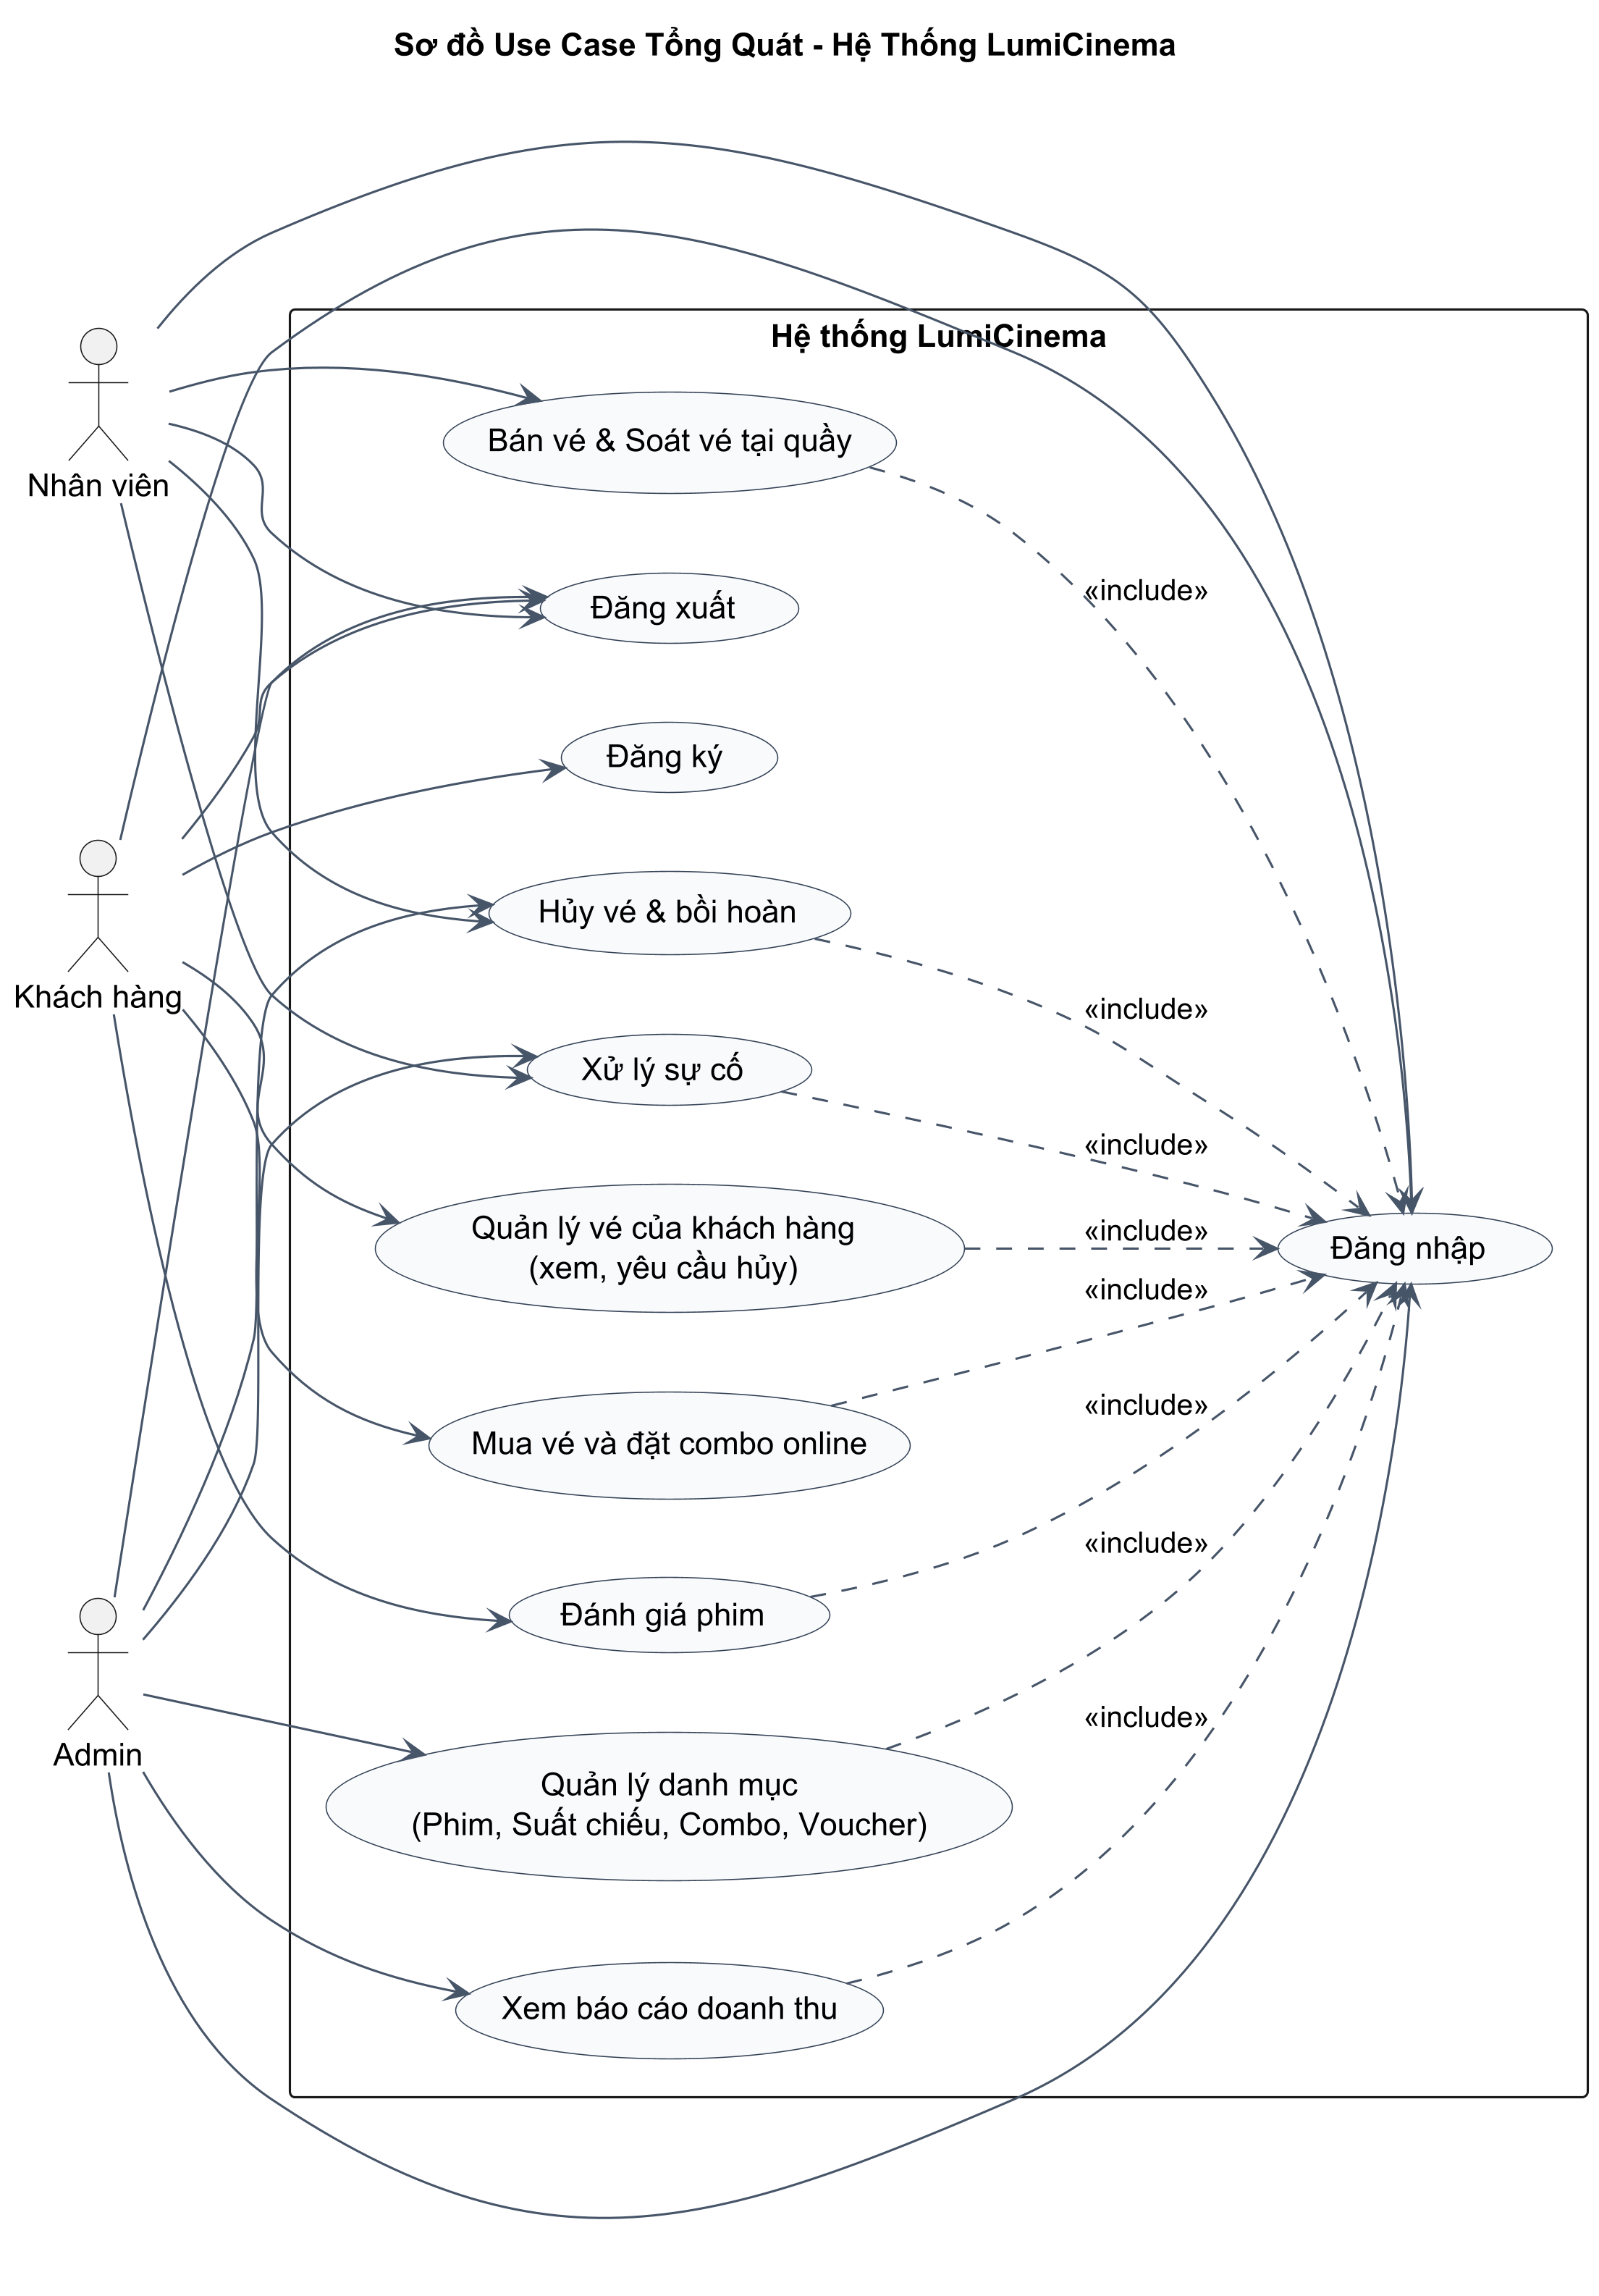
\includegraphics[width=\textwidth,height=0.80\textheight,keepaspectratio]{images/usecase/01_usecase_tong_quat.png}
  \caption{Sơ đồ Use Case Tổng Quát - Hệ Thống LumiCinema}
  \label{fig:uc_01}
\end{figure}

\begin{figure}[H]
  \centering
  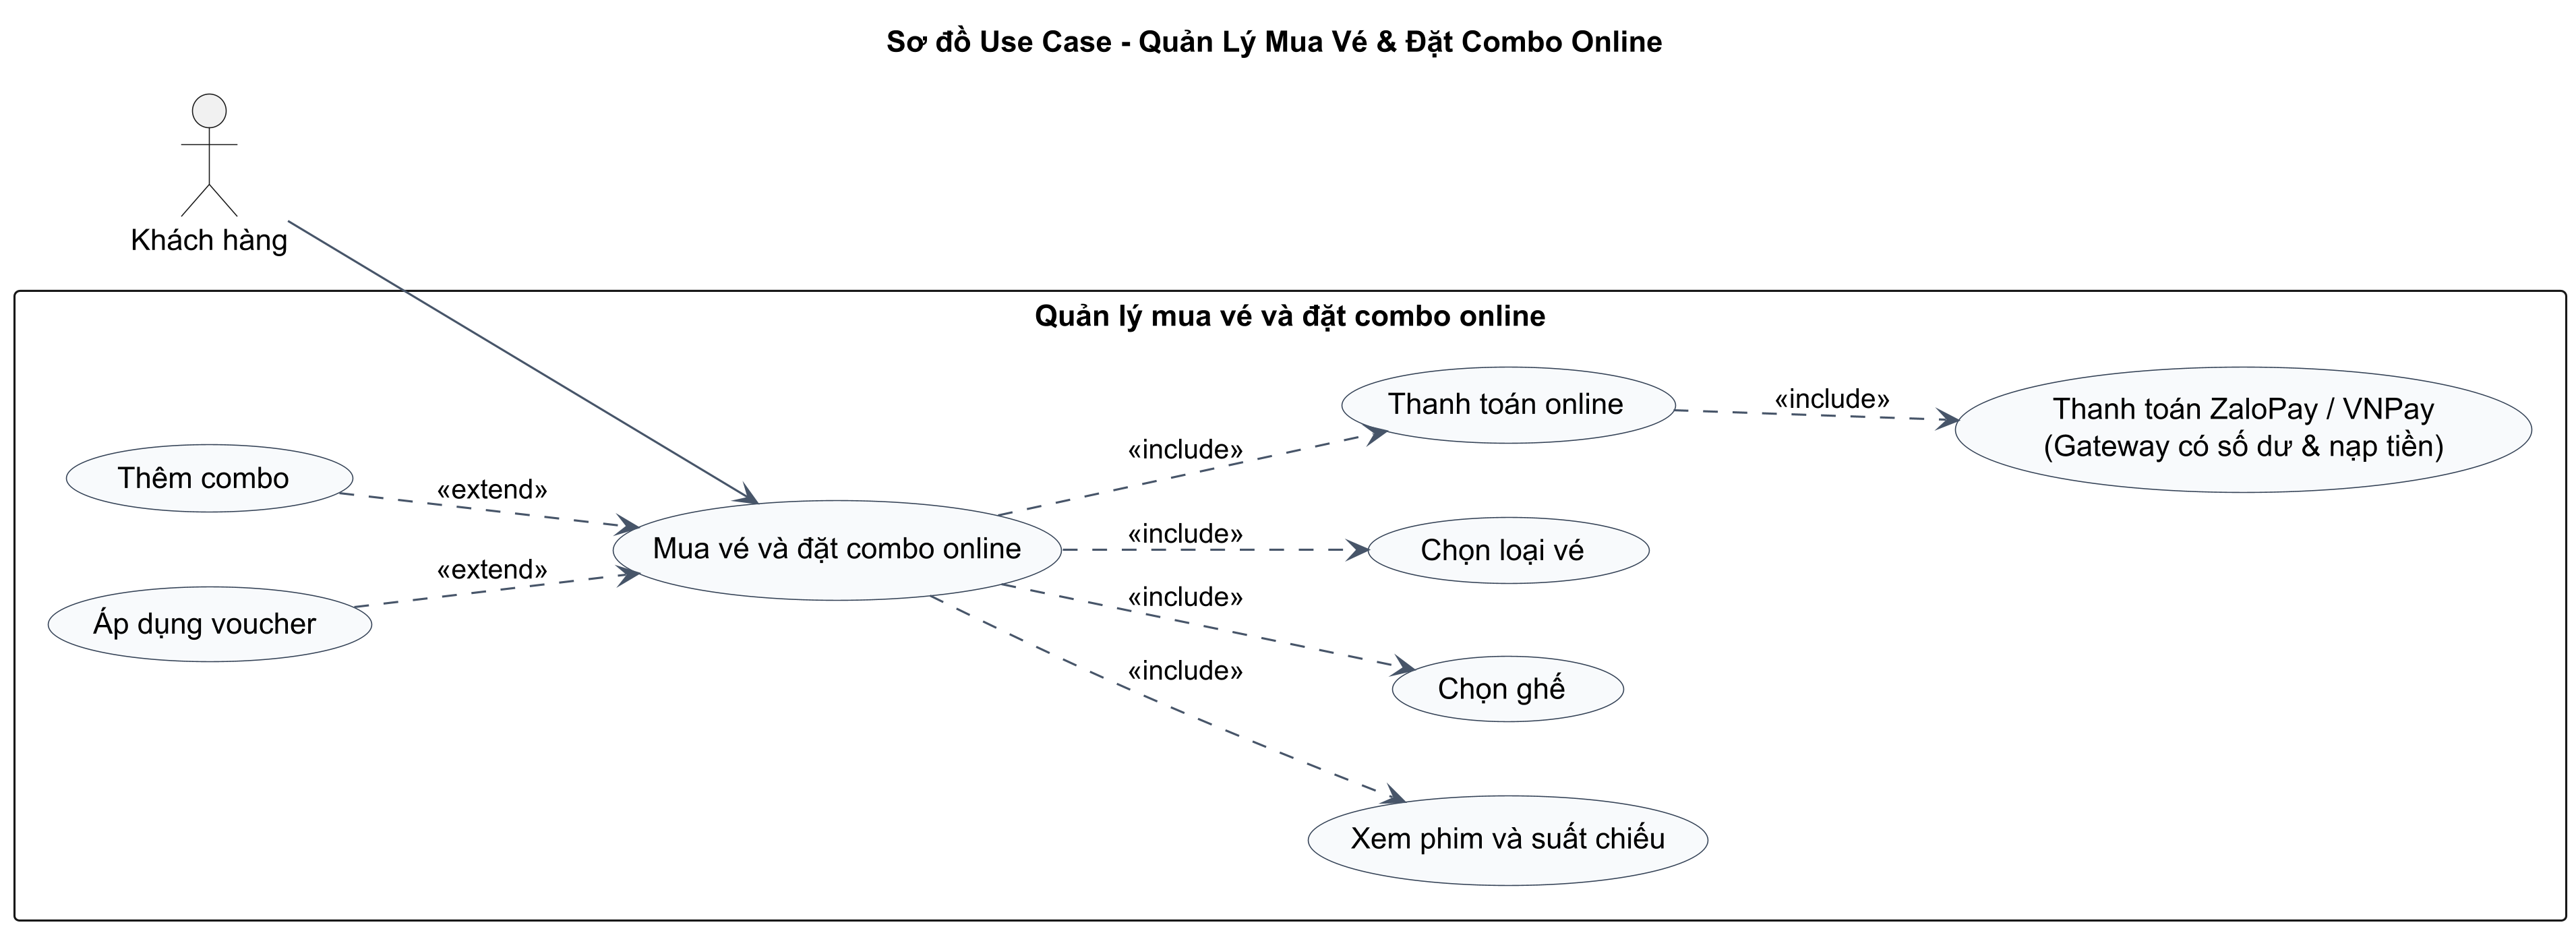
\includegraphics[width=\textwidth,height=0.80\textheight,keepaspectratio]{images/usecase/02_usecase_mua_ve_dat_combo_online.png}
  \caption{Sơ đồ Use Case - Quản Lý Mua Vé \& Đặt Combo Online}
  \label{fig:uc_02}
\end{figure}

\begin{figure}[H]
  \centering
  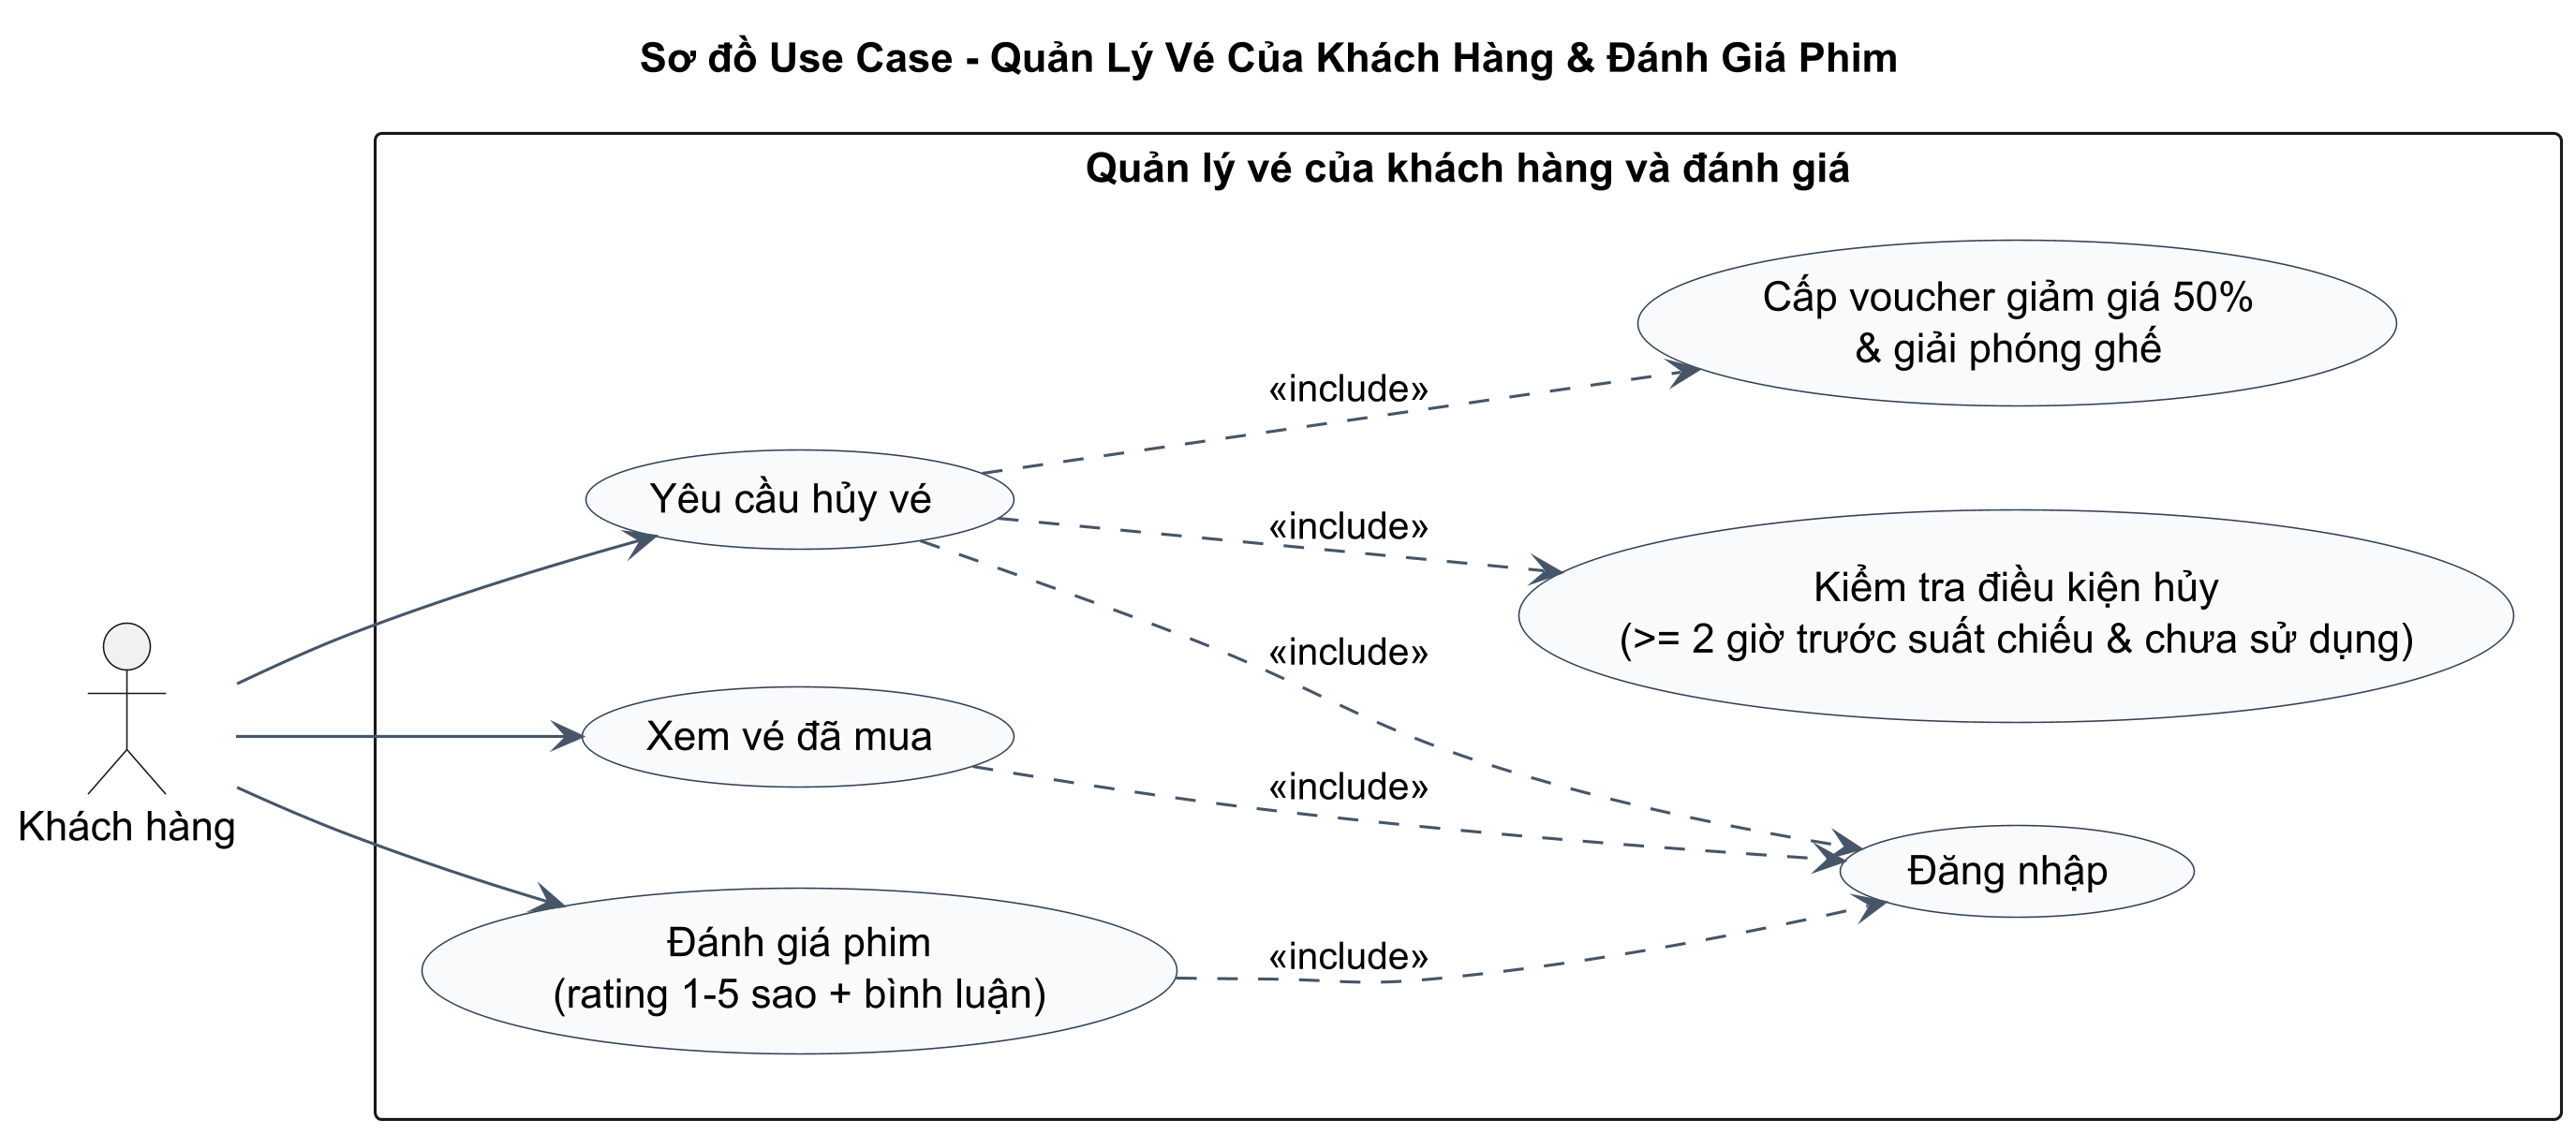
\includegraphics[width=\textwidth,height=0.80\textheight,keepaspectratio]{images/usecase/03_usecase_quan_ly_ve_va_danh_gia.png}
  \caption{Sơ đồ Use Case - Quản Lý Vé Của Khách Hàng \& Đánh Giá Phim}
  \label{fig:uc_03}
\end{figure}

\begin{figure}[H]
  \centering
  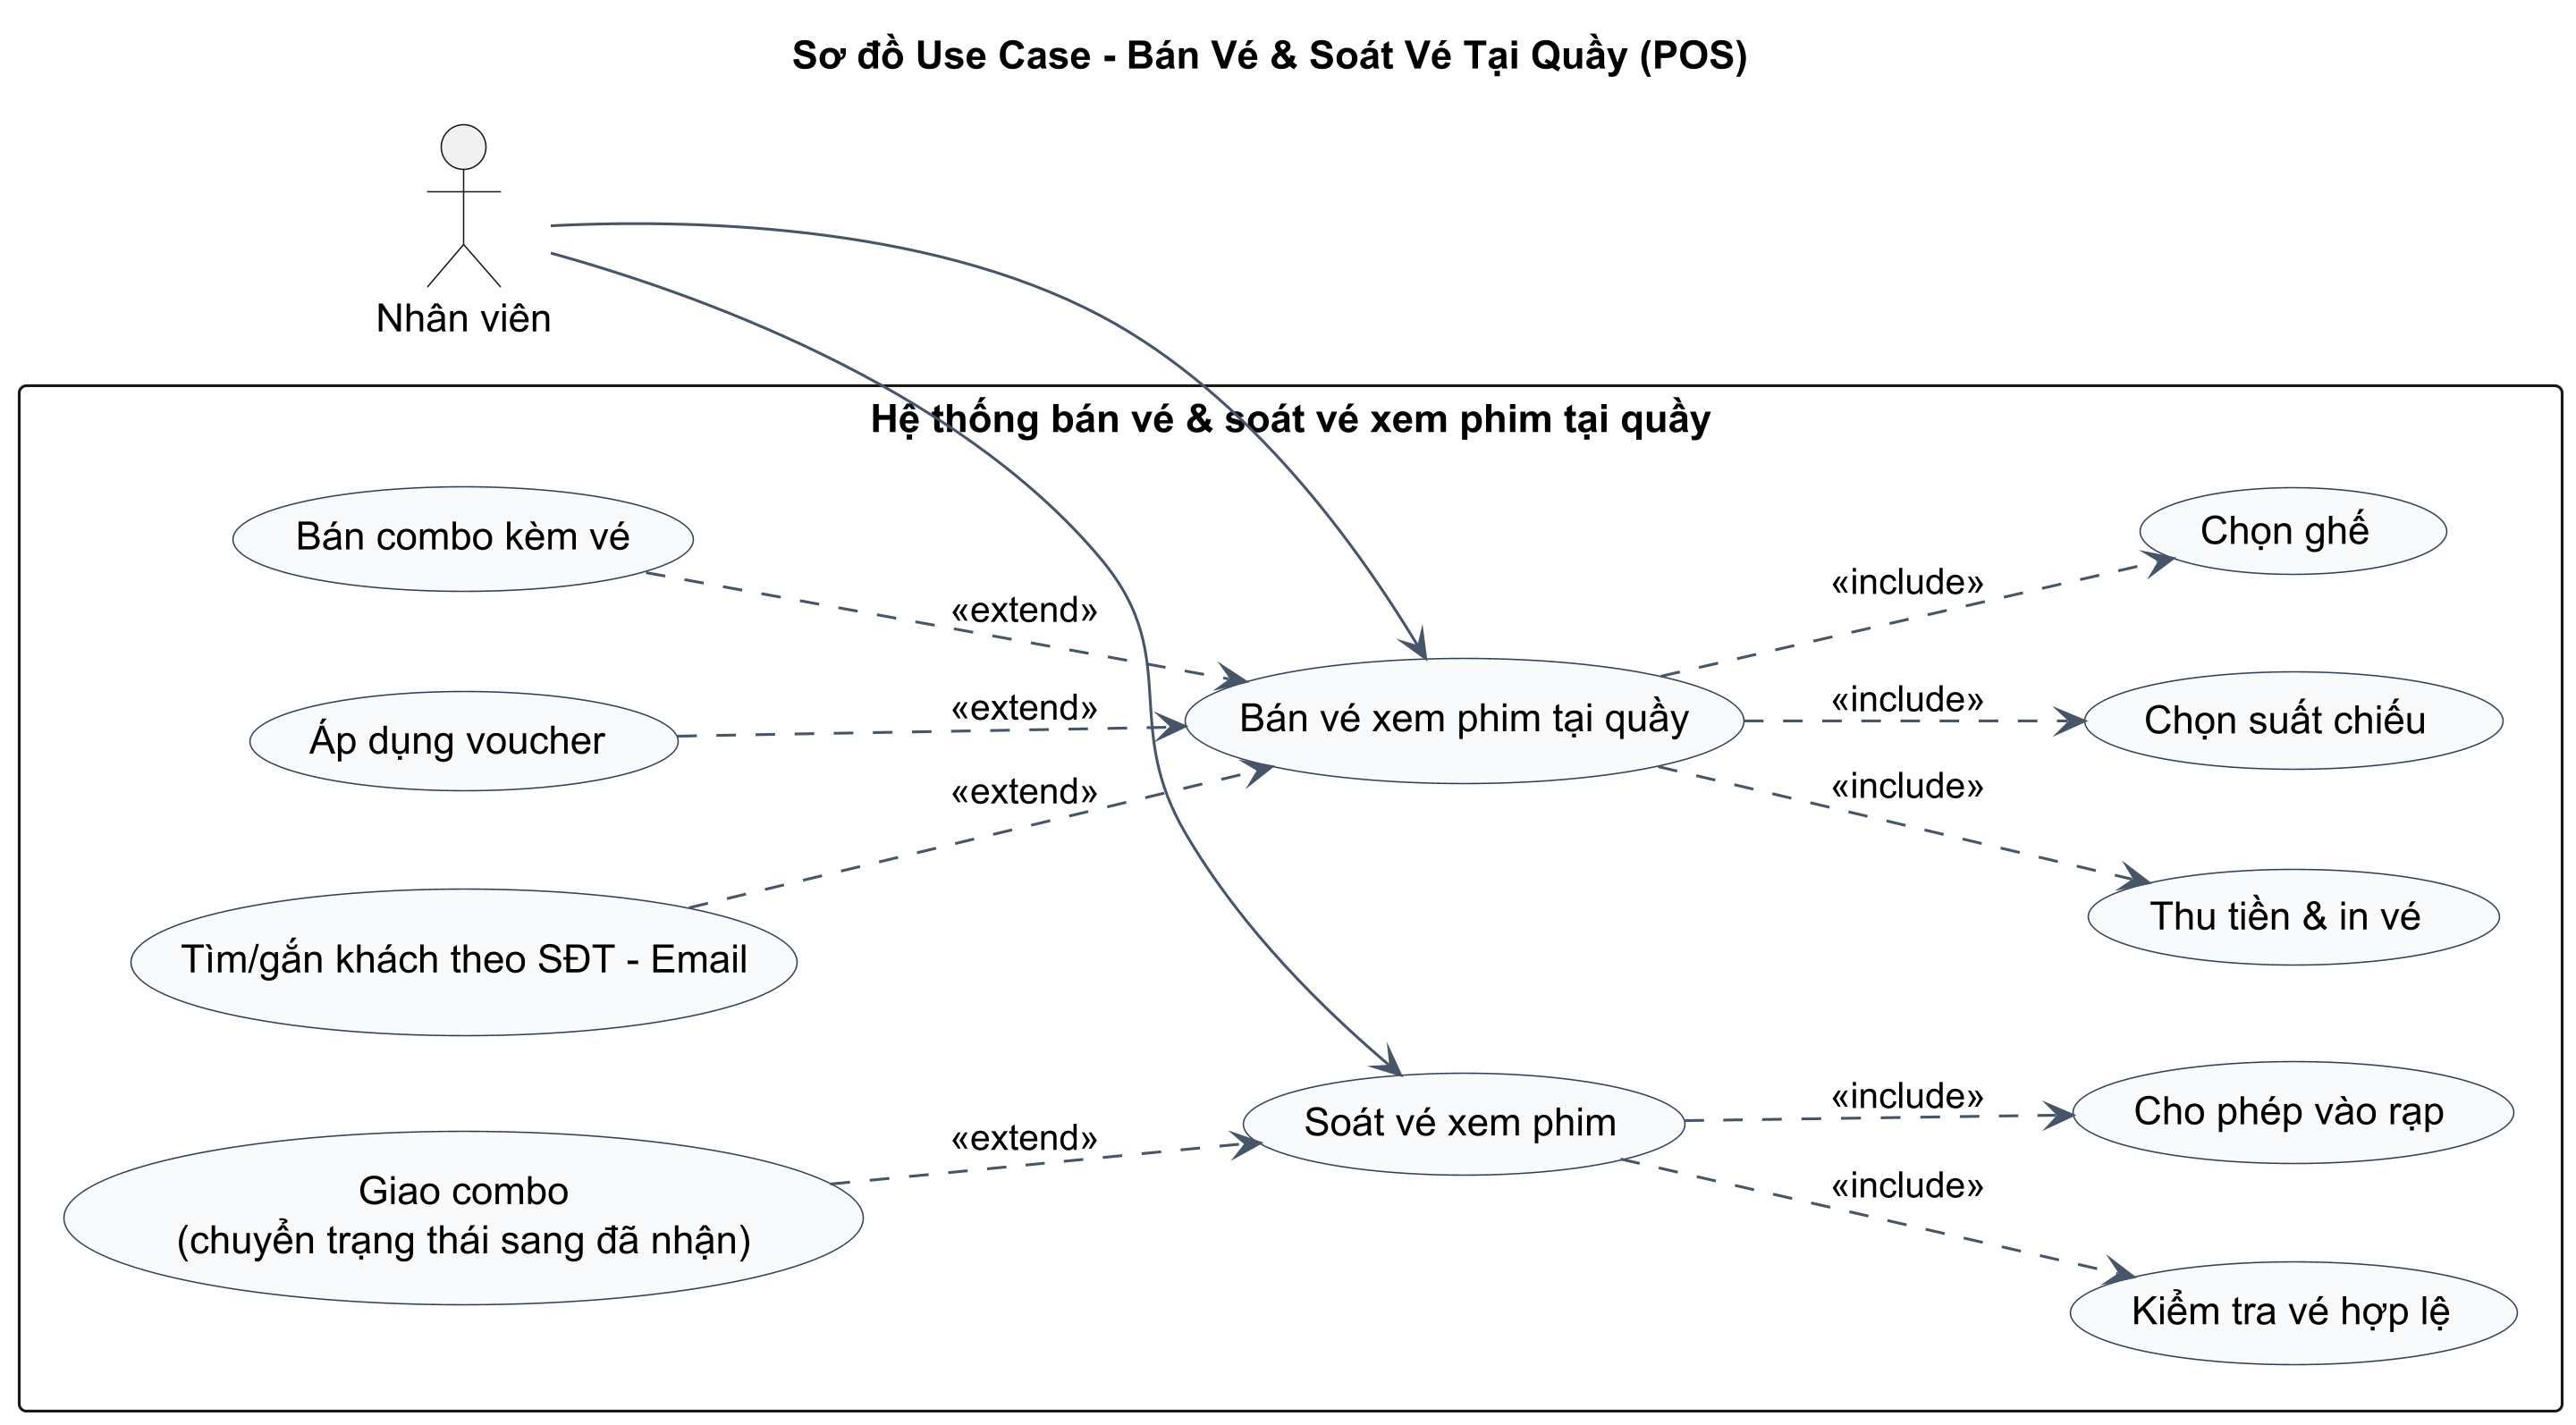
\includegraphics[width=\textwidth,height=0.80\textheight,keepaspectratio]{images/usecase/04_usecase_ban_ve_soat_ve_tai_quay.png}
  \caption{Sơ đồ Use Case - Bán Vé \& Soát Vé Tại Quầy (POS)}
  \label{fig:uc_04}
\end{figure}

\begin{figure}[H]
  \centering
  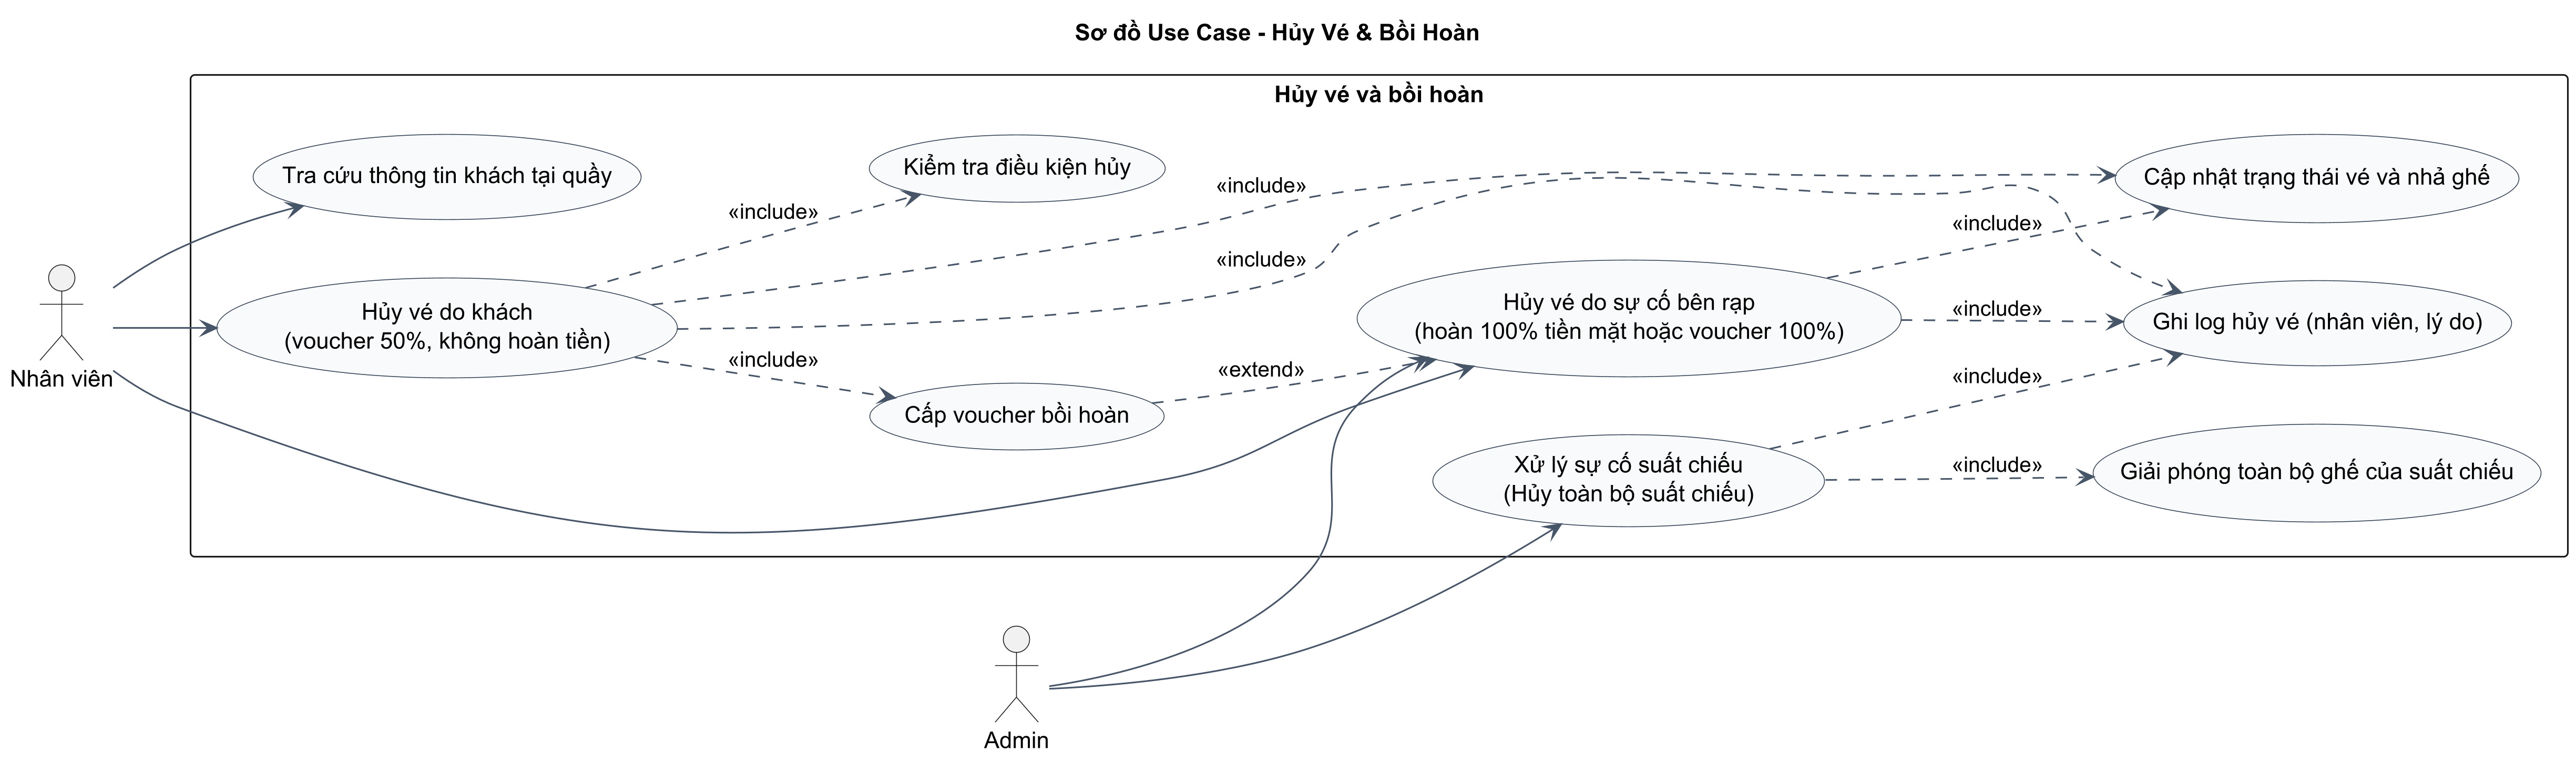
\includegraphics[width=\textwidth,height=0.80\textheight,keepaspectratio]{images/usecase/05_usecase_huy_ve_va_boi_hoan.png}
  \caption{Sơ đồ Use Case - Hủy Vé \& Bồi Hoàn}
  \label{fig:uc_05}
\end{figure}

\begin{figure}[H]
  \centering
  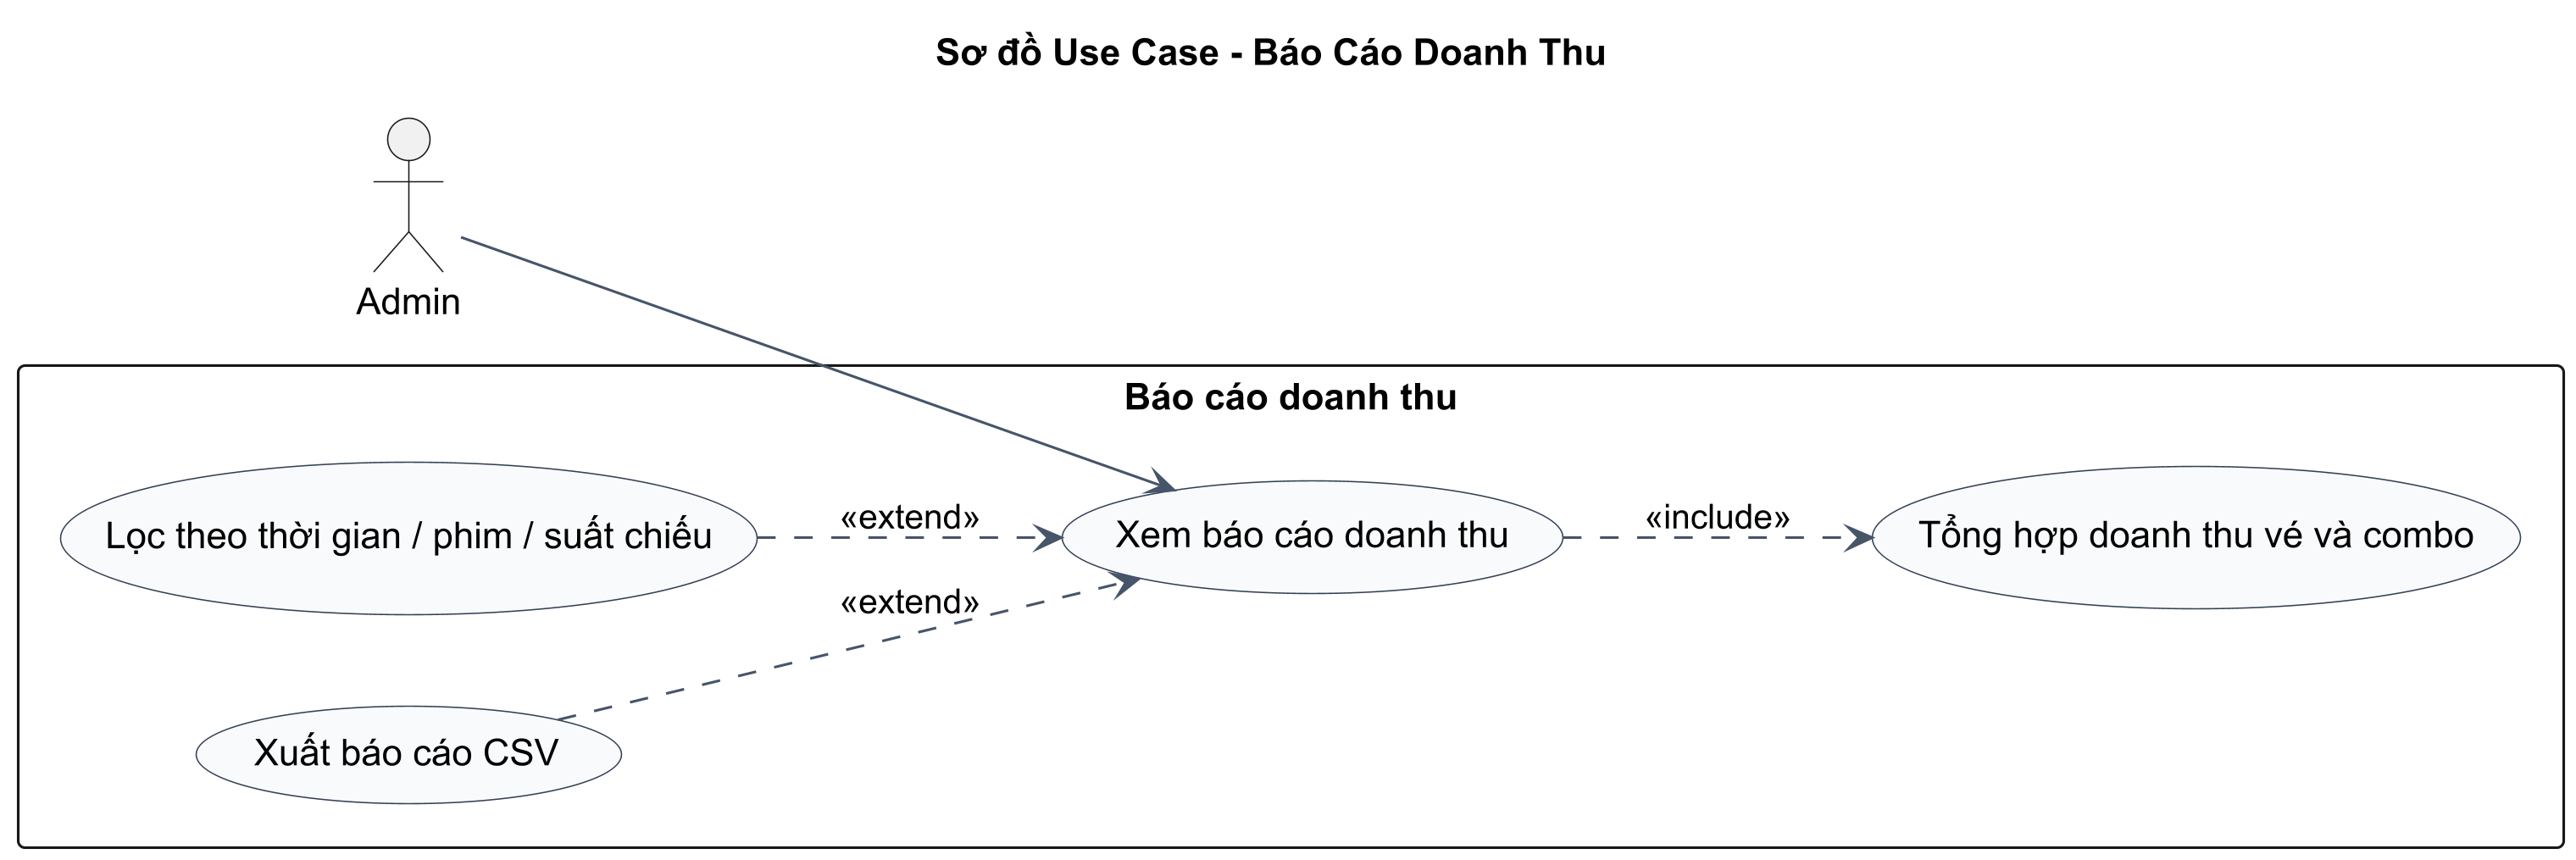
\includegraphics[width=\textwidth,height=0.80\textheight,keepaspectratio]{images/usecase/06_usecase_bao_cao_doanh_thu.png}
  \caption{Sơ đồ Use Case - Báo Cáo Doanh Thu}
  \label{fig:uc_06}
\end{figure}

\begin{figure}[H]
  \centering
  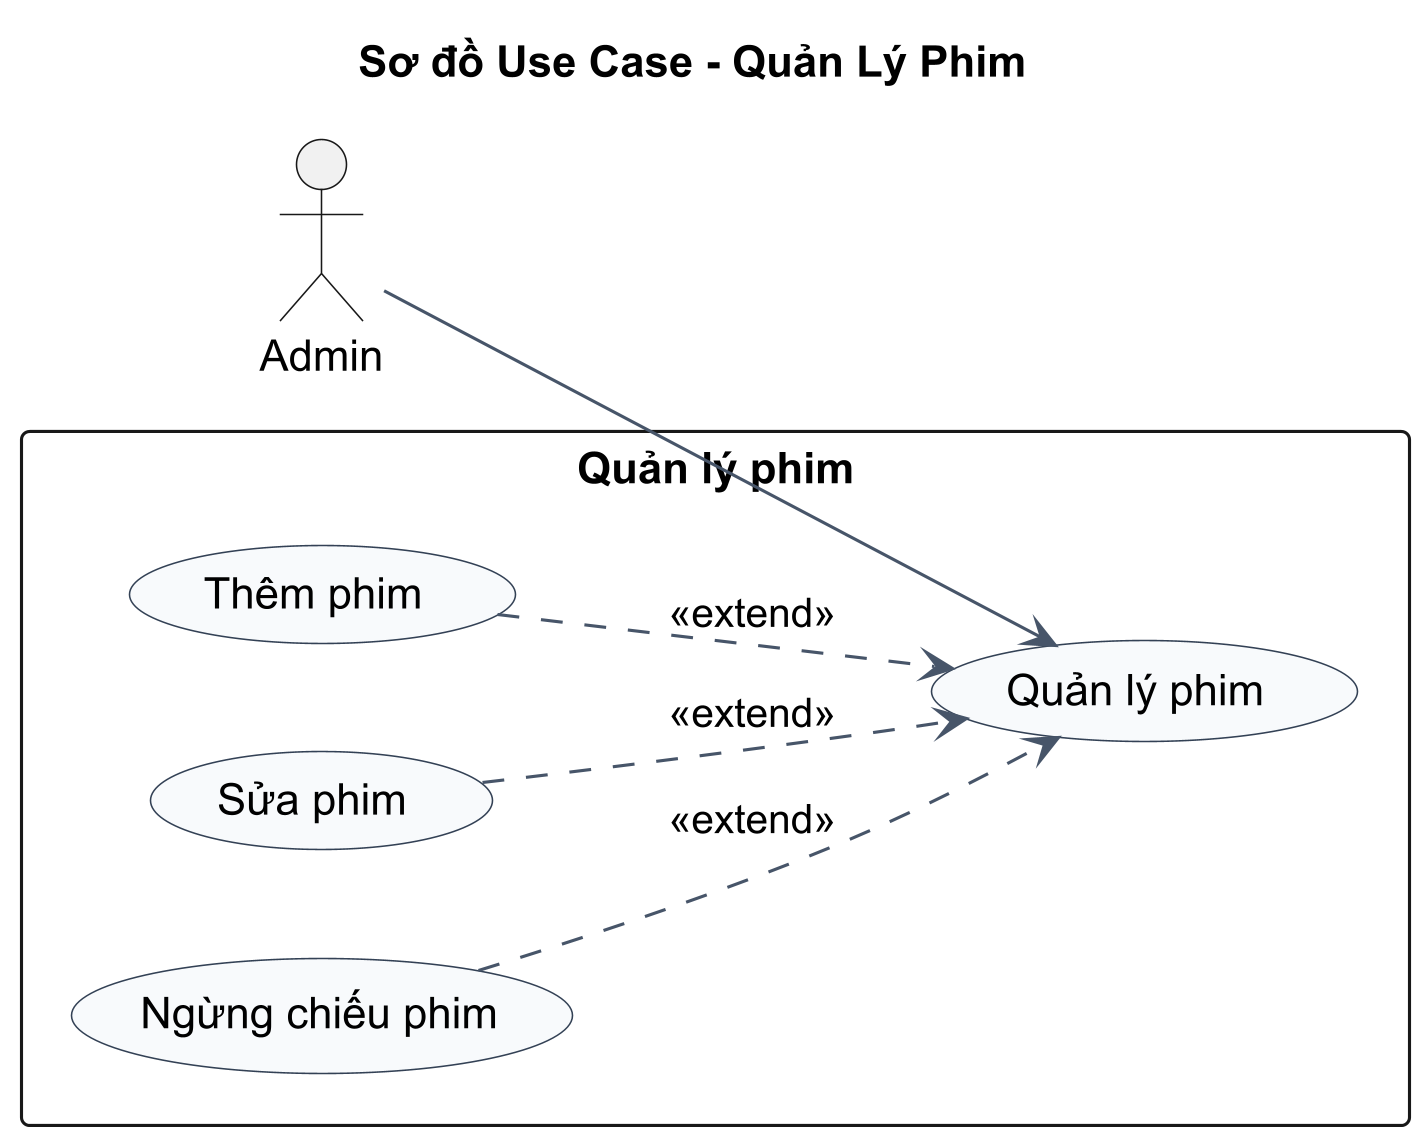
\includegraphics[width=\textwidth,height=0.80\textheight,keepaspectratio]{images/usecase/07_usecase_quan_ly_phim.png}
  \caption{Sơ đồ Use Case - Quản Lý Phim}
  \label{fig:uc_07}
\end{figure}

\begin{figure}[H]
  \centering
  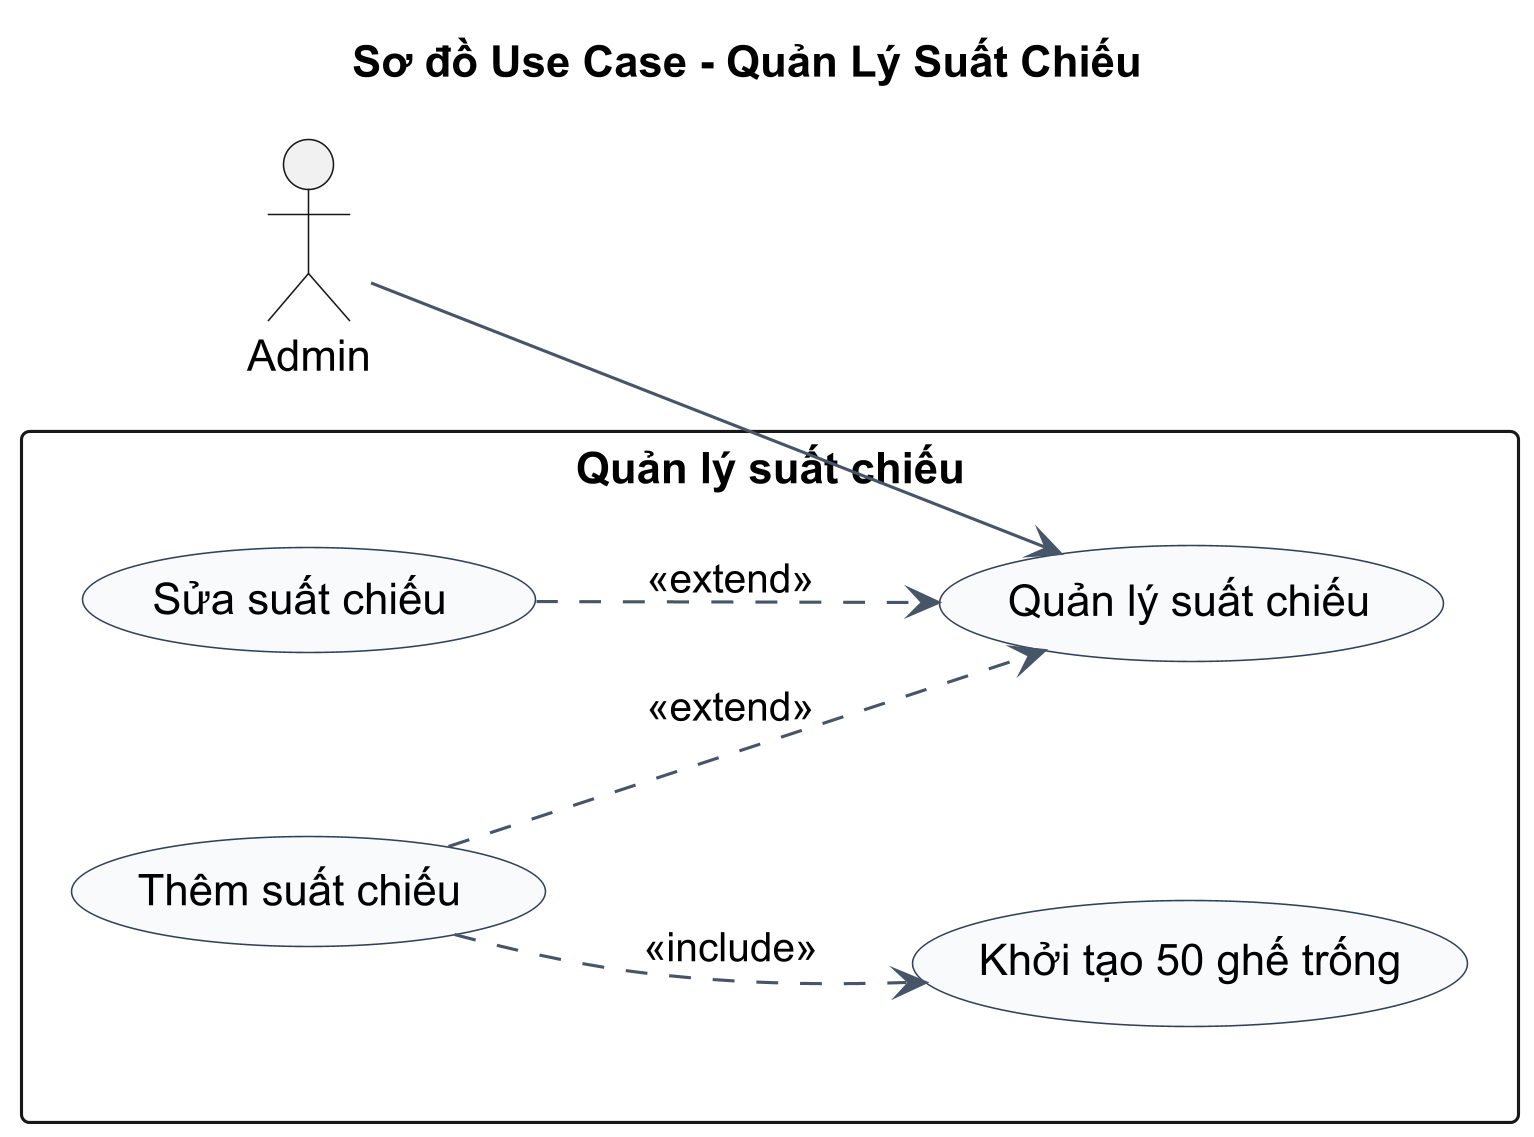
\includegraphics[width=\textwidth,height=0.80\textheight,keepaspectratio]{images/usecase/08_usecase_quan_ly_suat_chieu.png}
  \caption{Sơ đồ Use Case - Quản Lý Suất Chiếu}
  \label{fig:uc_08}
\end{figure}

\begin{figure}[H]
  \centering
  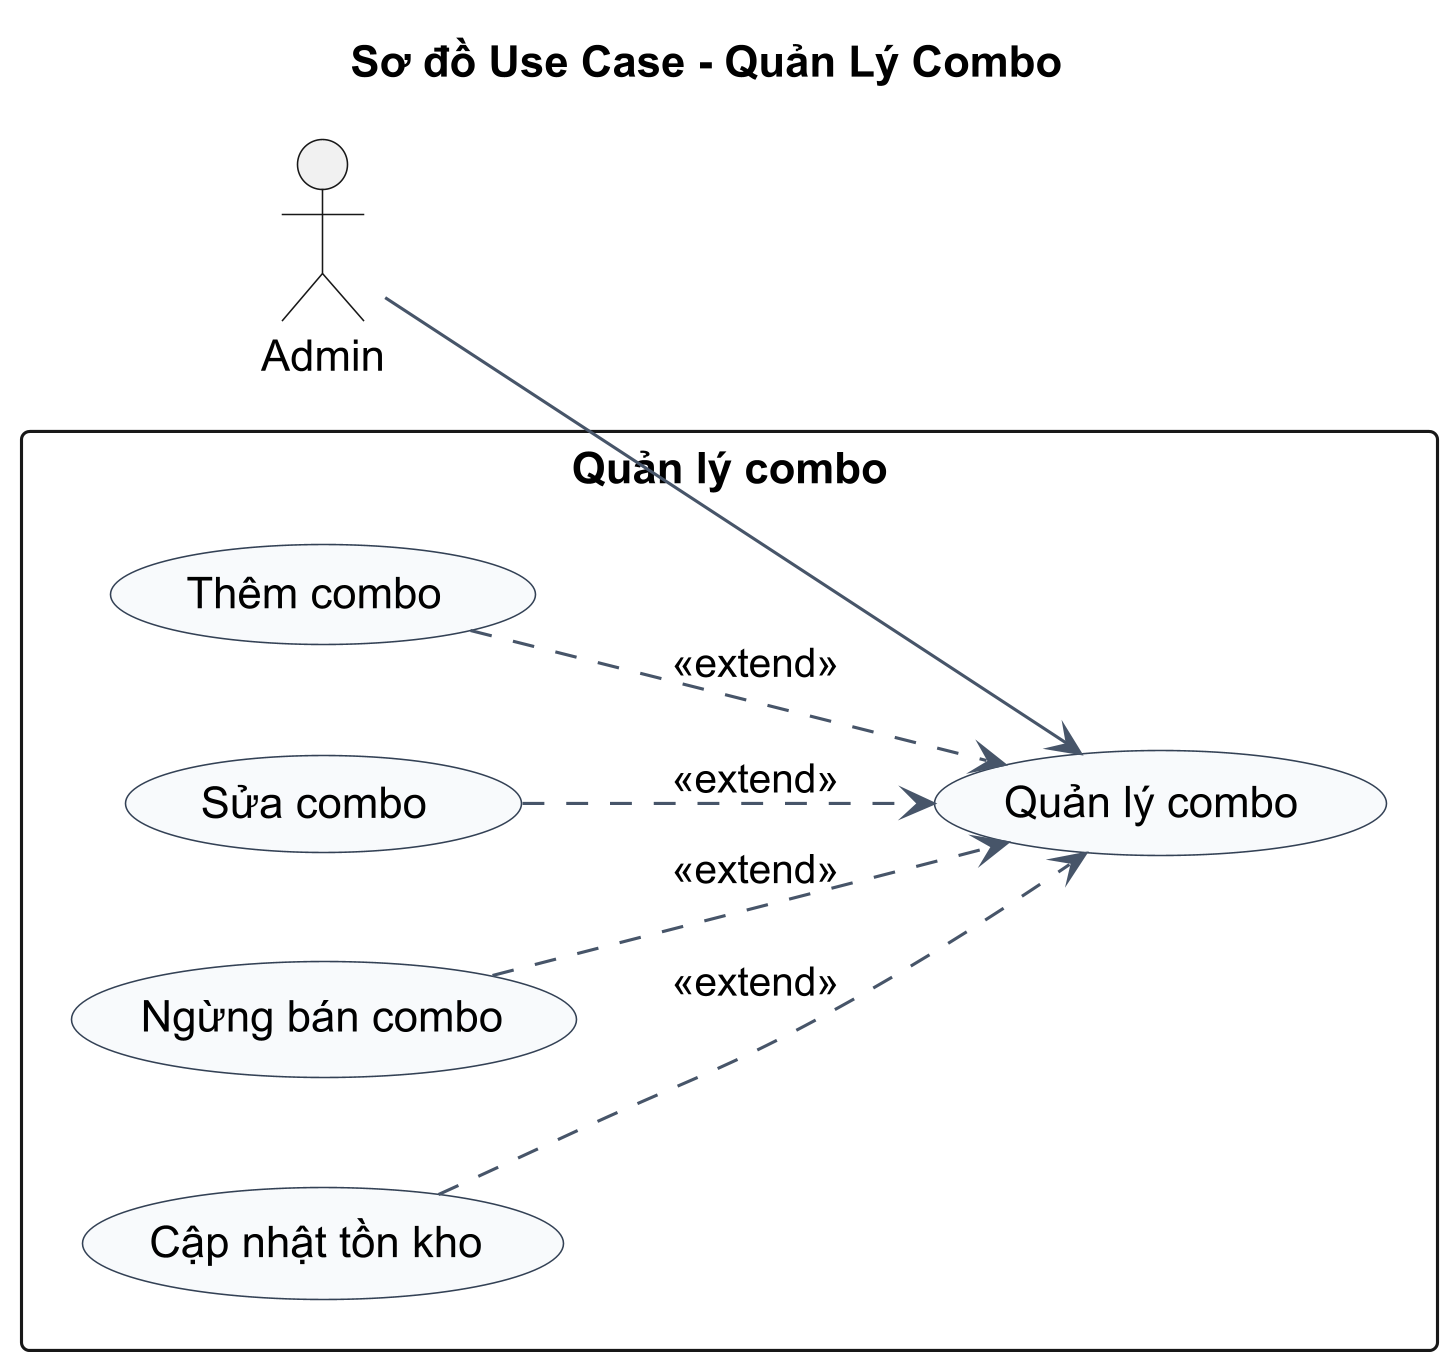
\includegraphics[width=\textwidth,height=0.80\textheight,keepaspectratio]{images/usecase/09_usecase_quan_ly_combo.png}
  \caption{Sơ đồ Use Case - Quản Lý Combo}
  \label{fig:uc_09}
\end{figure}

\begin{figure}[H]
  \centering
  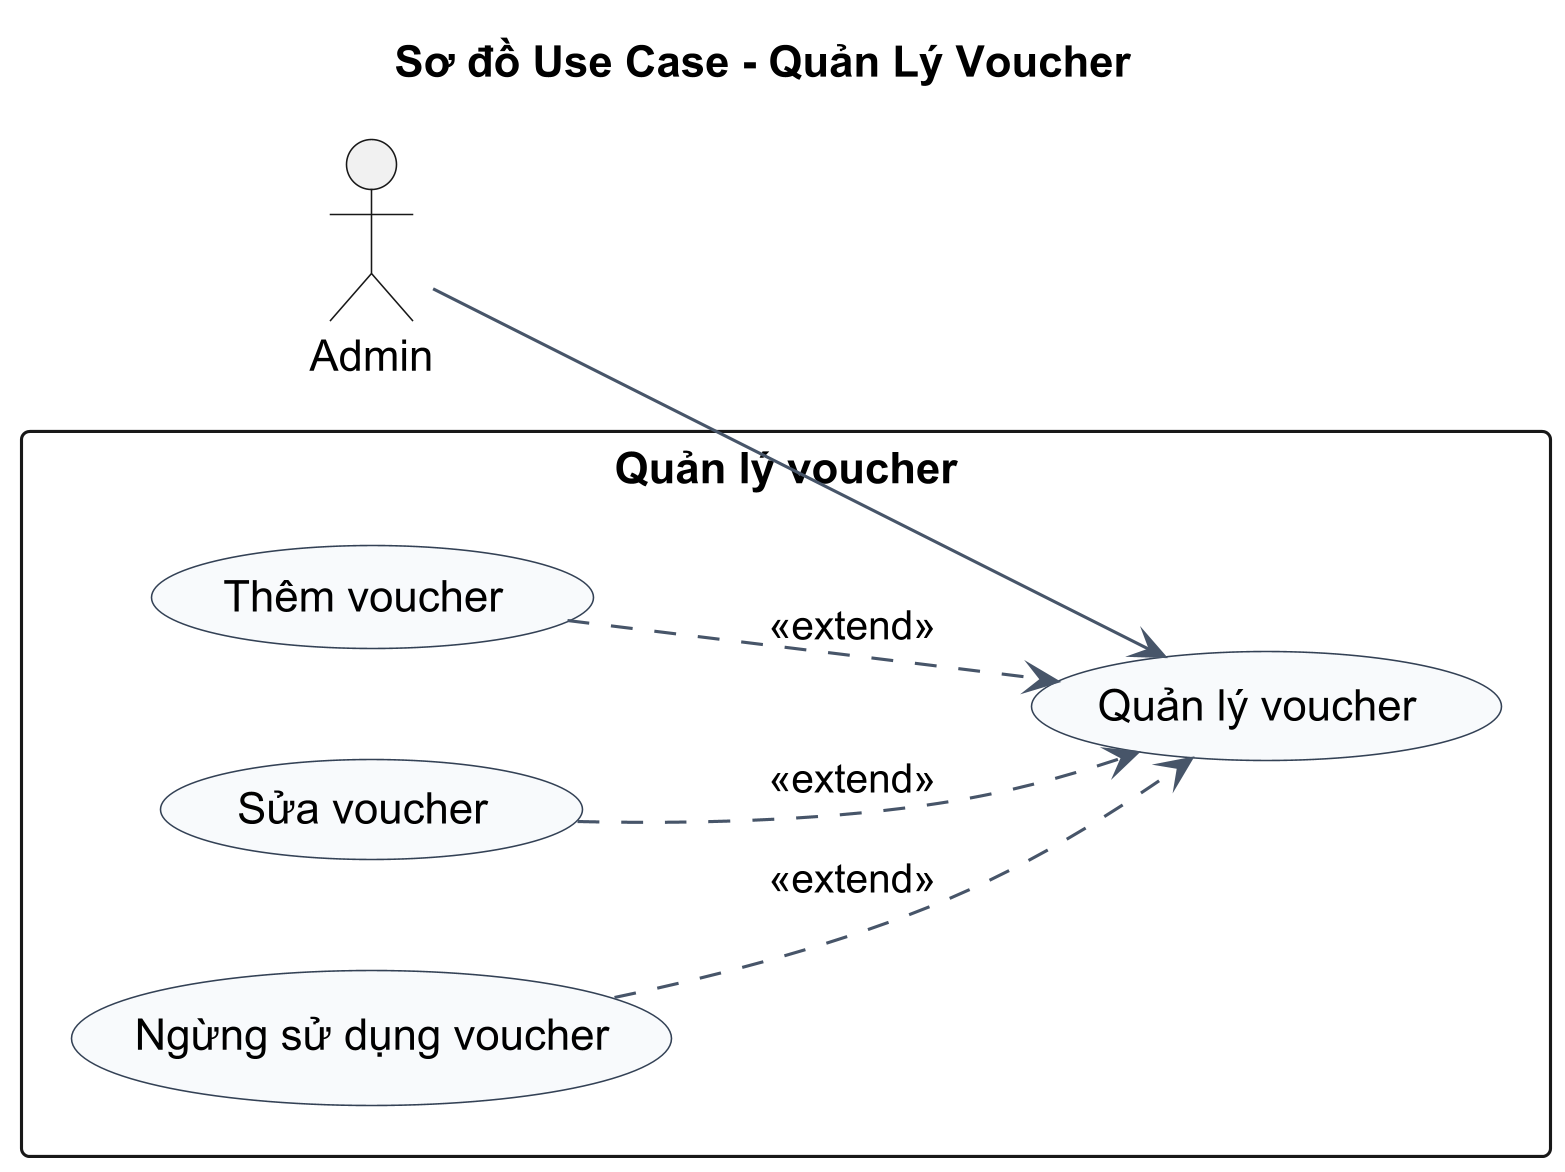
\includegraphics[width=\textwidth,height=0.80\textheight,keepaspectratio]{images/usecase/10_usecase_quan_ly_voucher.png}
  \caption{Sơ đồ Use Case - Quản Lý Voucher}
  \label{fig:uc_10}
\end{figure}

\subsection{Đặc tả chi tiết các Use Case}
\begin{longtable}{|p{4.2cm}|p{11.3cm}|}
\hline
\rowcolor{headerblue} \textbf{Tên Use Case} & \textbf{Quản lý vé khách hàng} \\ \hline
\endhead
\textbf{Tác nhân chính} & Admin / Người quản lý \\ \hline
\textbf{Tóm tắt} & Use Case bắt đầu khi Người quản lý truy cập chức năng quản lý vé khách hàng để xem danh sách vé, tra cứu vé, kiểm tra trạng thái và xem chi tiết vé. \\ \hline
\textbf{Dòng sự kiện chính} & 1. Người quản lý đăng nhập vào hệ thống.\newline 2. Người quản lý chọn chức năng Quản lý vé khách hàng.\newline 3. Hệ thống hiển thị giao diện quản lý vé.\newline 4. Người quản lý chọn xem danh sách vé, tra cứu vé khách hàng hoặc xem trạng thái vé.\newline 5. Người quản lý nhập thông tin tra cứu nếu cần.\newline 6. Hệ thống tìm kiếm và hiển thị kết quả phù hợp.\newline 7. Người quản lý chọn một vé để xem chi tiết.\newline 8. Hệ thống hiển thị mã vé, thông tin khách hàng, phim, suất chiếu, phòng chiếu, ghế, giá vé và trạng thái vé. \\ \hline
\textbf{Dòng sự kiện phụ} & 1. Không tìm thấy vé: hệ thống thông báo không có kết quả phù hợp.\newline 2. Người quản lý không có quyền: hệ thống từ chối truy cập.\newline 3. Thông tin tra cứu không hợp lệ: hệ thống yêu cầu kiểm tra lại.\newline 4. Lỗi truy vấn dữ liệu: hệ thống thông báo không thể tải thông tin vé. \\ \hline
\textbf{Tiền điều kiện} & Người quản lý đã đăng nhập vào hệ thống và có quyền quản lý vé khách hàng. \\ \hline
\textbf{Hậu điều kiện} & Thông tin danh sách vé, kết quả tra cứu, trạng thái vé hoặc chi tiết vé được hiển thị theo yêu cầu của Người quản lý. \\ \hline
\end{longtable}

\begin{longtable}{|p{4.2cm}|p{11.3cm}|}
\hline
\rowcolor{headerblue} \textbf{Tóm tắt} & \textbf{Use Case bắt đầu khi Người quản lý chọn chức năng xem danh sách vé khách hàng.} \\ \hline
\endhead
\textbf{Dòng sự kiện chính} & 1. Người quản lý truy cập chức năng Quản lý vé khách hàng.\newline 2. Người quản lý chọn Xem danh sách vé.\newline 3. Hệ thống truy vấn dữ liệu vé.\newline 4. Hệ thống hiển thị mã vé, khách hàng, phim, suất chiếu, phòng chiếu, ghế ngồi, giá vé và trạng thái vé. \\ \hline
\textbf{Dòng sự kiện phụ} & 1. Danh sách vé trống: hệ thống thông báo chưa có dữ liệu vé.\newline 2. Lỗi truy vấn: hệ thống thông báo không thể tải danh sách vé. \\ \hline
\textbf{Tiền điều kiện} & Người quản lý đã đăng nhập và có quyền xem danh sách vé. \\ \hline
\textbf{Hậu điều kiện} & Danh sách vé khách hàng được hiển thị trên giao diện quản lý. \\ \hline
\end{longtable}

\begin{longtable}{|p{4.2cm}|p{11.3cm}|}
\hline
\rowcolor{headerblue} \textbf{Tóm tắt} & \textbf{Use Case bắt đầu khi Người quản lý muốn tìm kiếm vé của một khách hàng cụ thể.} \\ \hline
\endhead
\textbf{Dòng sự kiện chính} & 1. Người quản lý chọn Tra cứu vé khách hàng.\newline 2. Hệ thống hiển thị giao diện tìm kiếm.\newline 3. Người quản lý nhập mã vé, email hoặc số điện thoại khách hàng.\newline 4. Người quản lý chọn Tìm kiếm.\newline 5. Hệ thống kiểm tra thông tin và truy vấn dữ liệu.\newline 6. Hệ thống hiển thị danh sách vé phù hợp. \\ \hline
\textbf{Dòng sự kiện phụ} & 1. Không tìm thấy vé: hệ thống thông báo không có kết quả.\newline 2. Thông tin tìm kiếm không hợp lệ: hệ thống yêu cầu nhập lại.\newline 3. Lỗi truy vấn: hệ thống thông báo tìm kiếm thất bại. \\ \hline
\textbf{Tiền điều kiện} & Người quản lý đã đăng nhập và có quyền tra cứu vé khách hàng. \\ \hline
\textbf{Hậu điều kiện} & Kết quả tra cứu vé được hiển thị để Người quản lý kiểm tra. \\ \hline
\end{longtable}


\section{Mô hình Sequence (Biểu đồ tuần tự)}
Hệ thống bao gồm 38 biểu đồ tuần tự (Sequence Diagram) mô tả chi tiết luồng tương tác giữa người dùng, giao diện (Frontend), các API Route (Backend), cơ sở dữ liệu (PostgreSQL/Prisma) và các dịch vụ tích hợp (ZaloPay/VNPay Gateway, Email SMTP).

\subsection{SƠ ĐỒ TUẦN TỰ: ĐĂNG KÝ TÀI KHOẢN KHÁCH HÀNG (CUSTOMER SIGN UP)}
\begin{figure}[H]
  \centering
  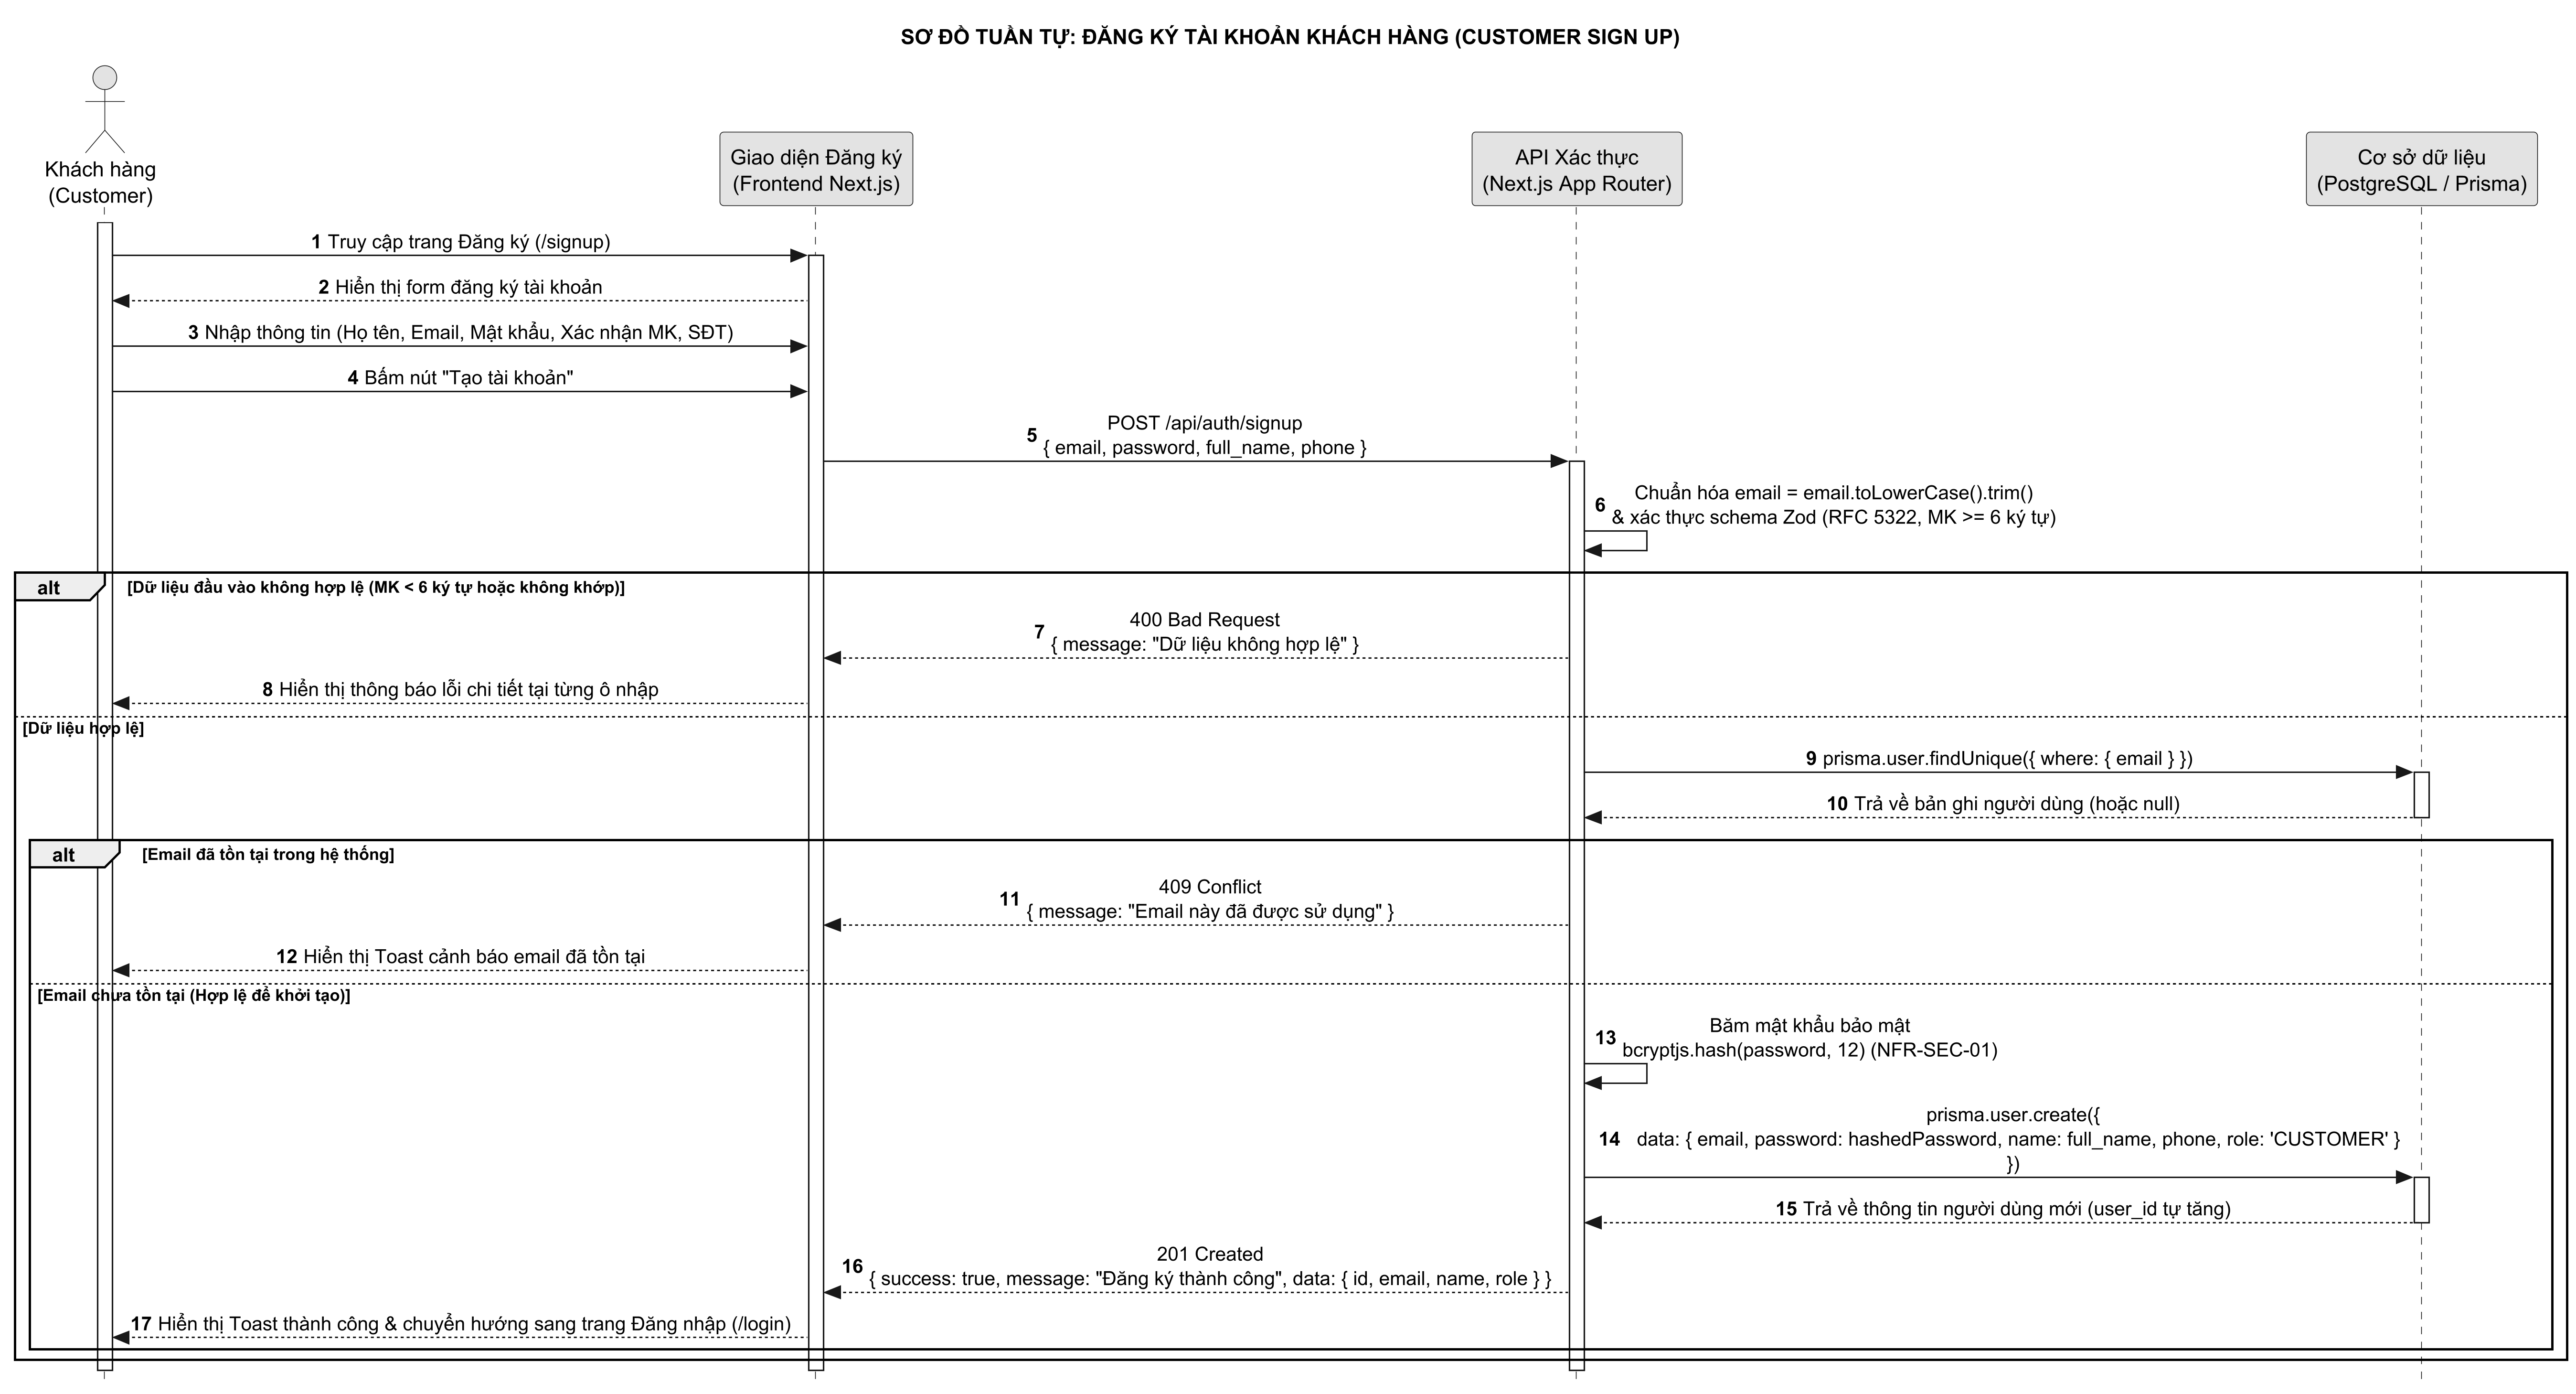
\includegraphics[width=\textwidth,height=0.80\textheight,keepaspectratio]{images/sequence/01_dang_ky_tai_khoan.png}
  \caption{Sequence Diagram: SƠ ĐỒ TUẦN TỰ: ĐĂNG KÝ TÀI KHOẢN KHÁCH HÀNG (CUSTOMER SIGN UP)}
  \label{fig:seq_01}
\end{figure}

\subsection{SƠ ĐỒ TUẦN TỰ: ĐĂNG NHẬP \& PHÂN QUYỀN ĐIỀU HƯỚNG (LOGIN \& RBAC ROUTING)}
\begin{figure}[H]
  \centering
  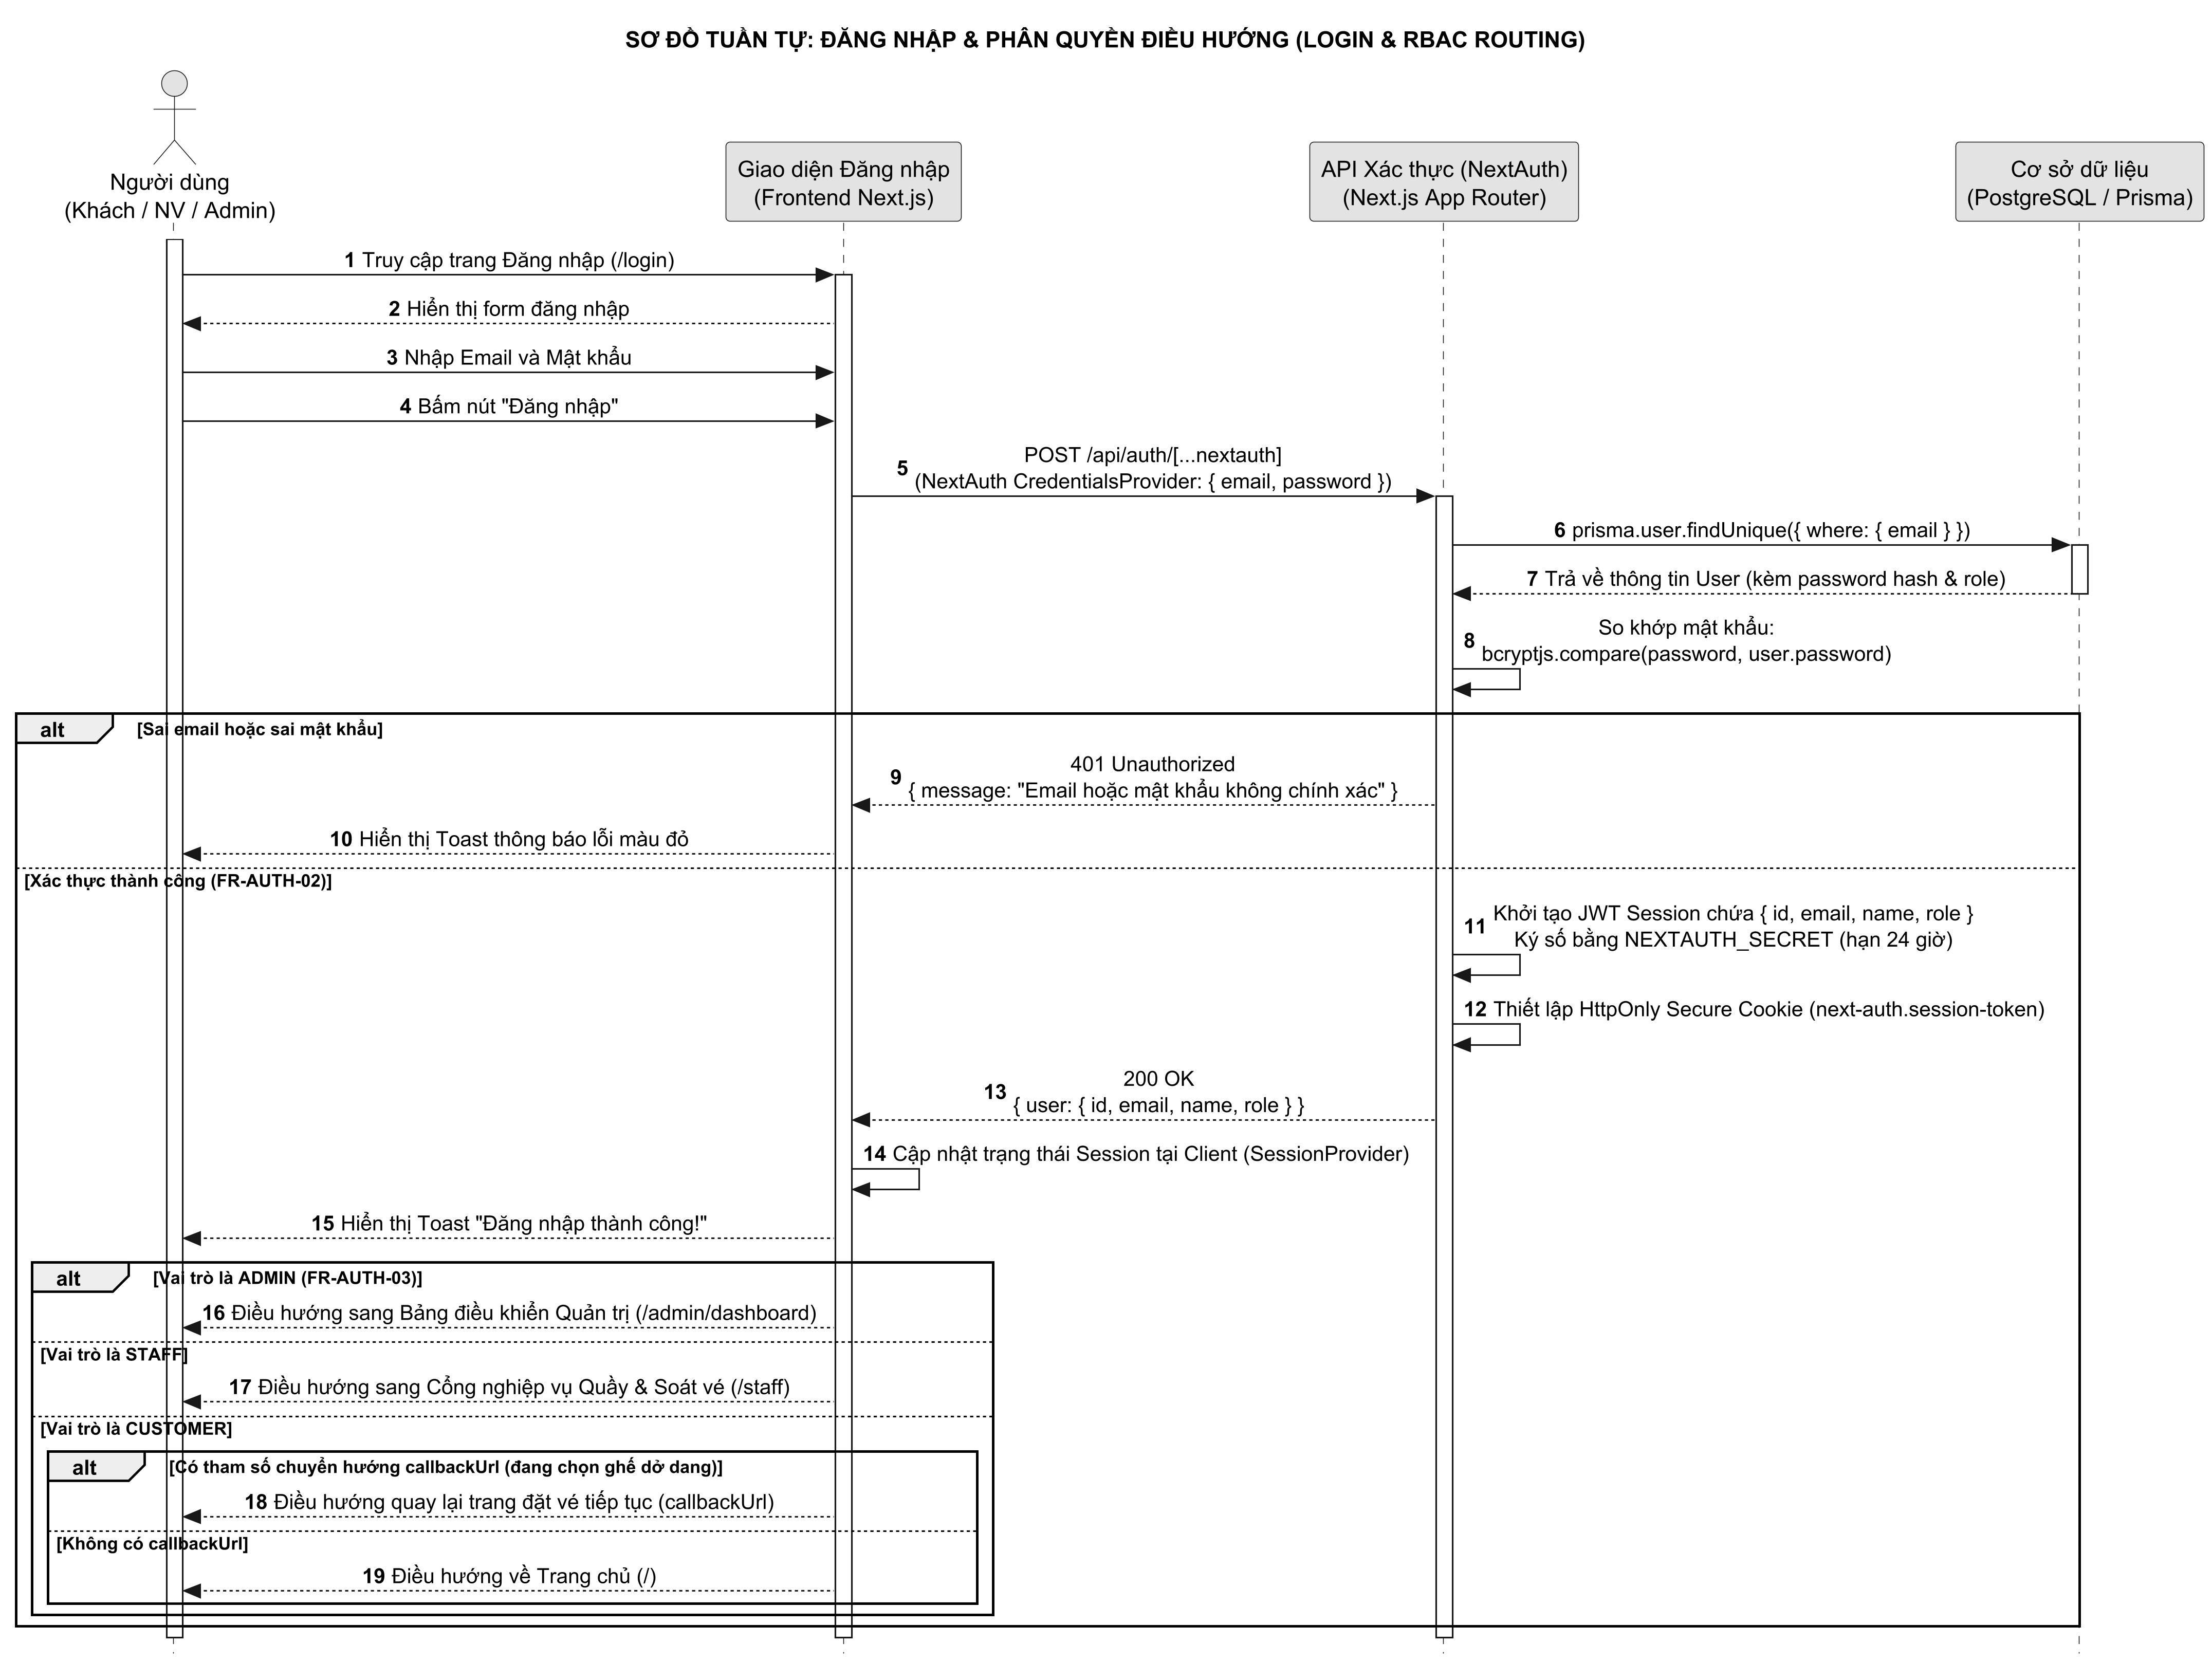
\includegraphics[width=\textwidth,height=0.80\textheight,keepaspectratio]{images/sequence/02_dang_nhap_he_thong.png}
  \caption{Sequence Diagram: SƠ ĐỒ TUẦN TỰ: ĐĂNG NHẬP \& PHÂN QUYỀN ĐIỀU HƯỚNG (LOGIN \& RBAC ROUTING)}
  \label{fig:seq_02}
\end{figure}

\subsection{SƠ ĐỒ TUẦN TỰ: ĐĂNG XUẤT HỆ THỐNG (LOGOUT / SIGN OUT)}
\begin{figure}[H]
  \centering
  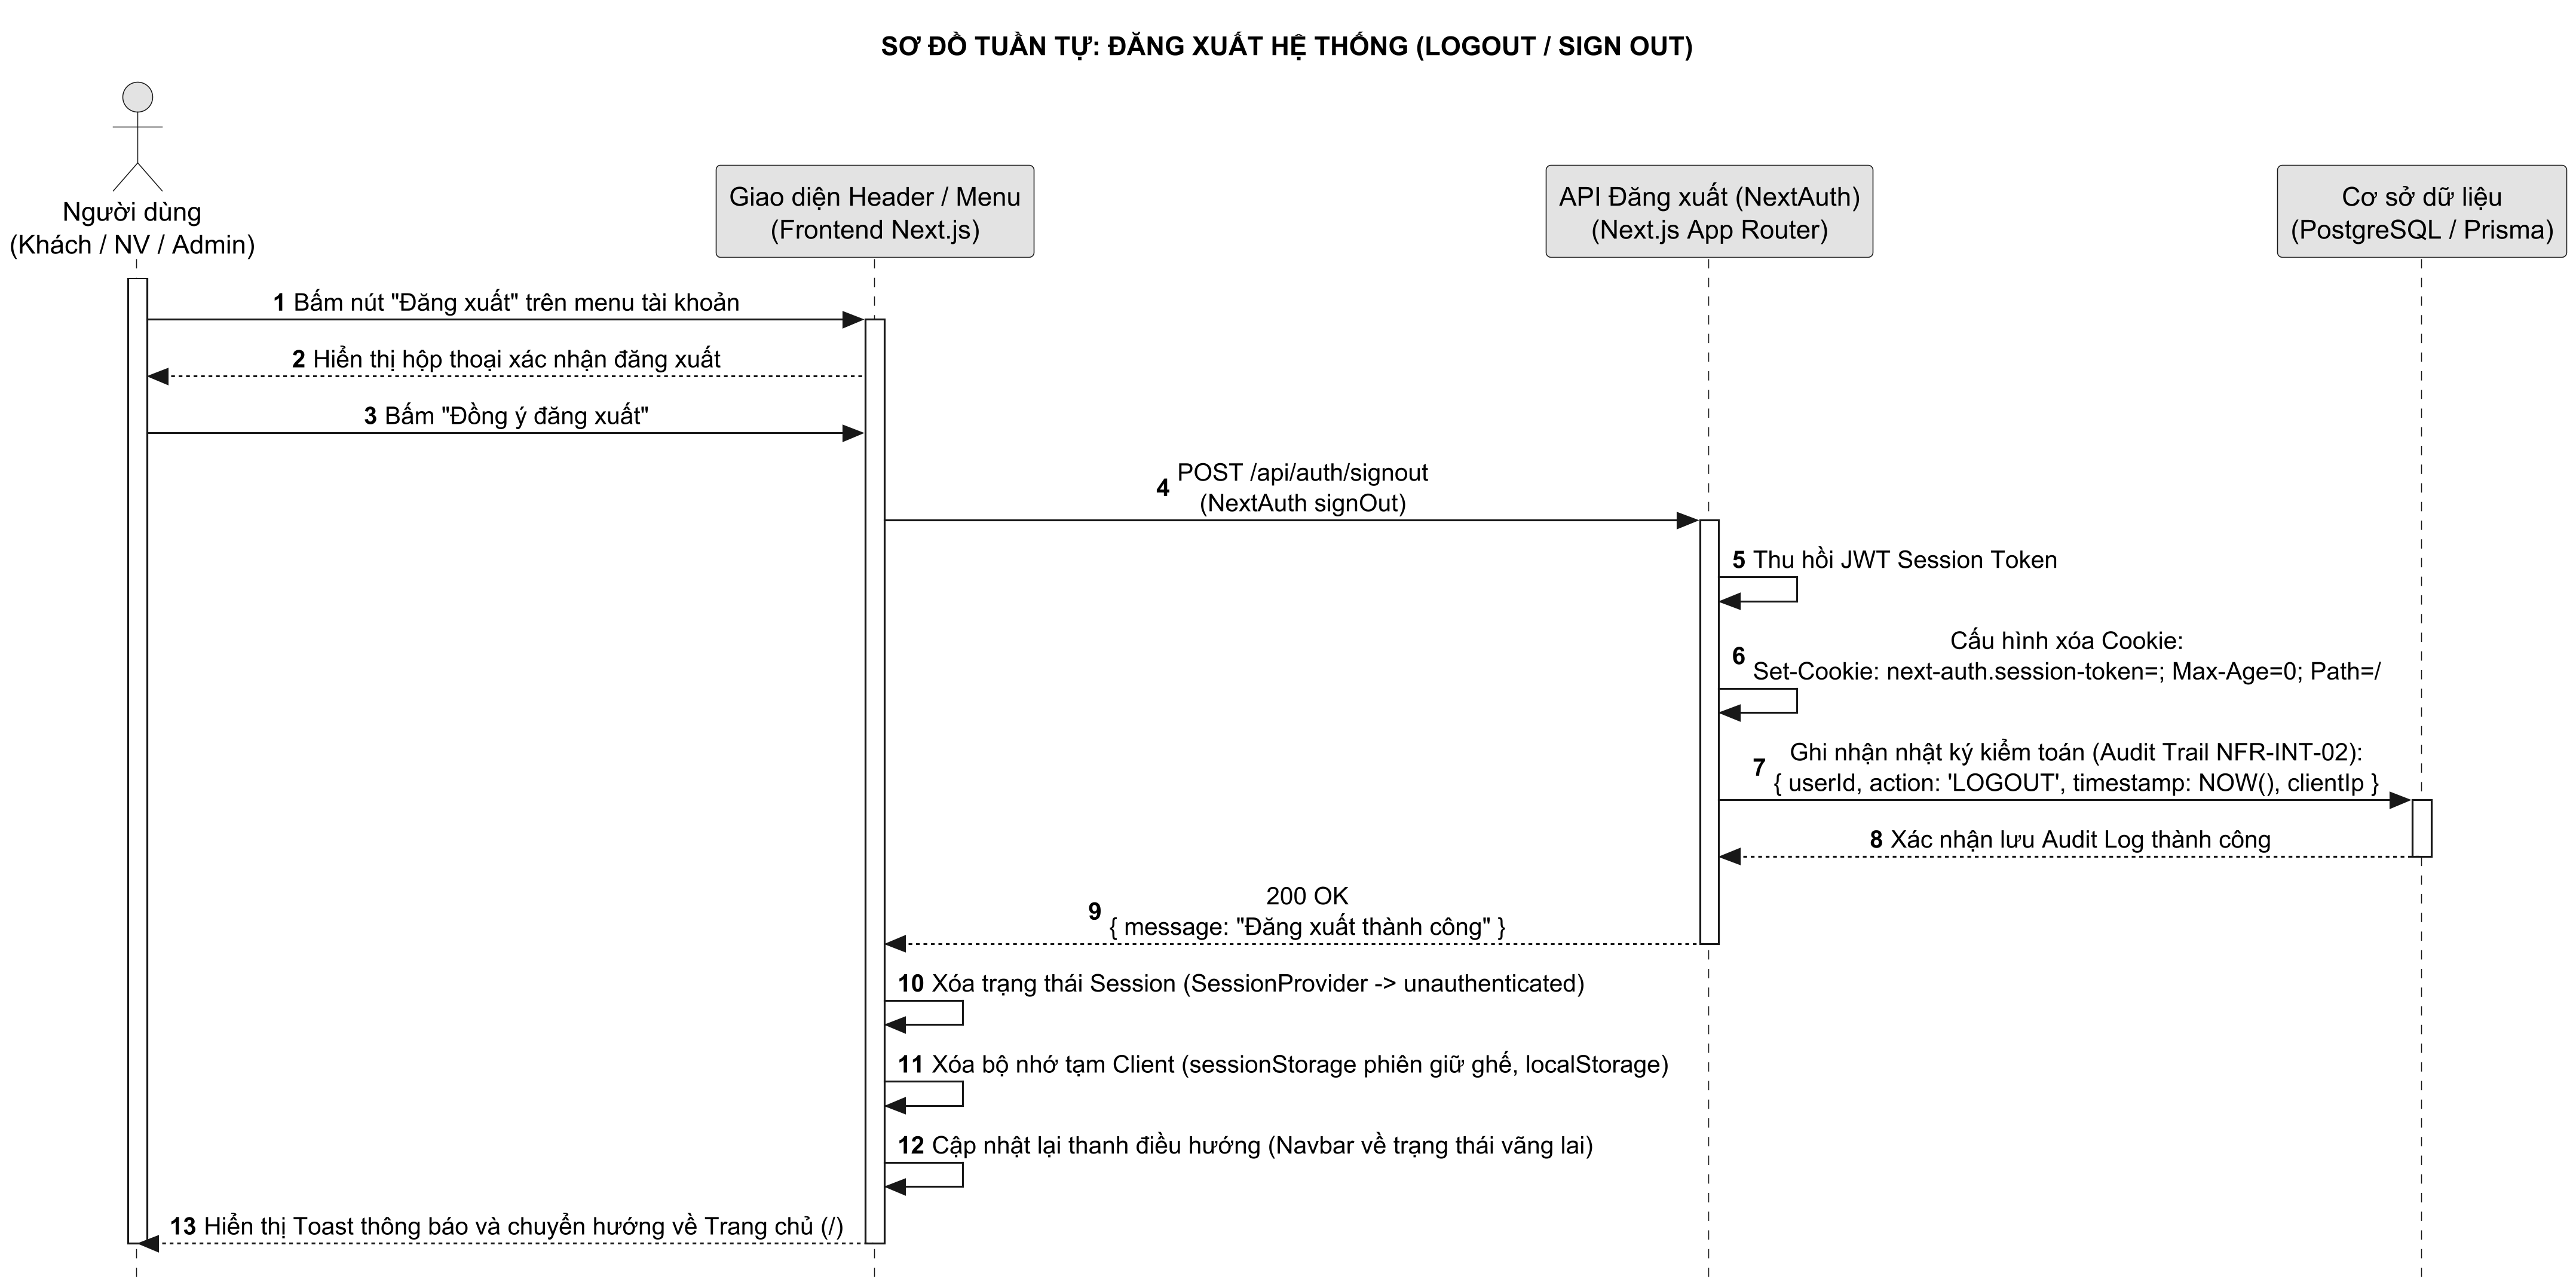
\includegraphics[width=\textwidth,height=0.80\textheight,keepaspectratio]{images/sequence/03_dang_xuat_he_thong.png}
  \caption{Sequence Diagram: SƠ ĐỒ TUẦN TỰ: ĐĂNG XUẤT HỆ THỐNG (LOGOUT / SIGN OUT)}
  \label{fig:seq_03}
\end{figure}

\subsection{SƠ ĐỒ TUẦN TỰ: MUA VÉ VÀ ĐẶT COMBO ONLINE (TỔNG QUAN)}
\begin{figure}[H]
  \centering
  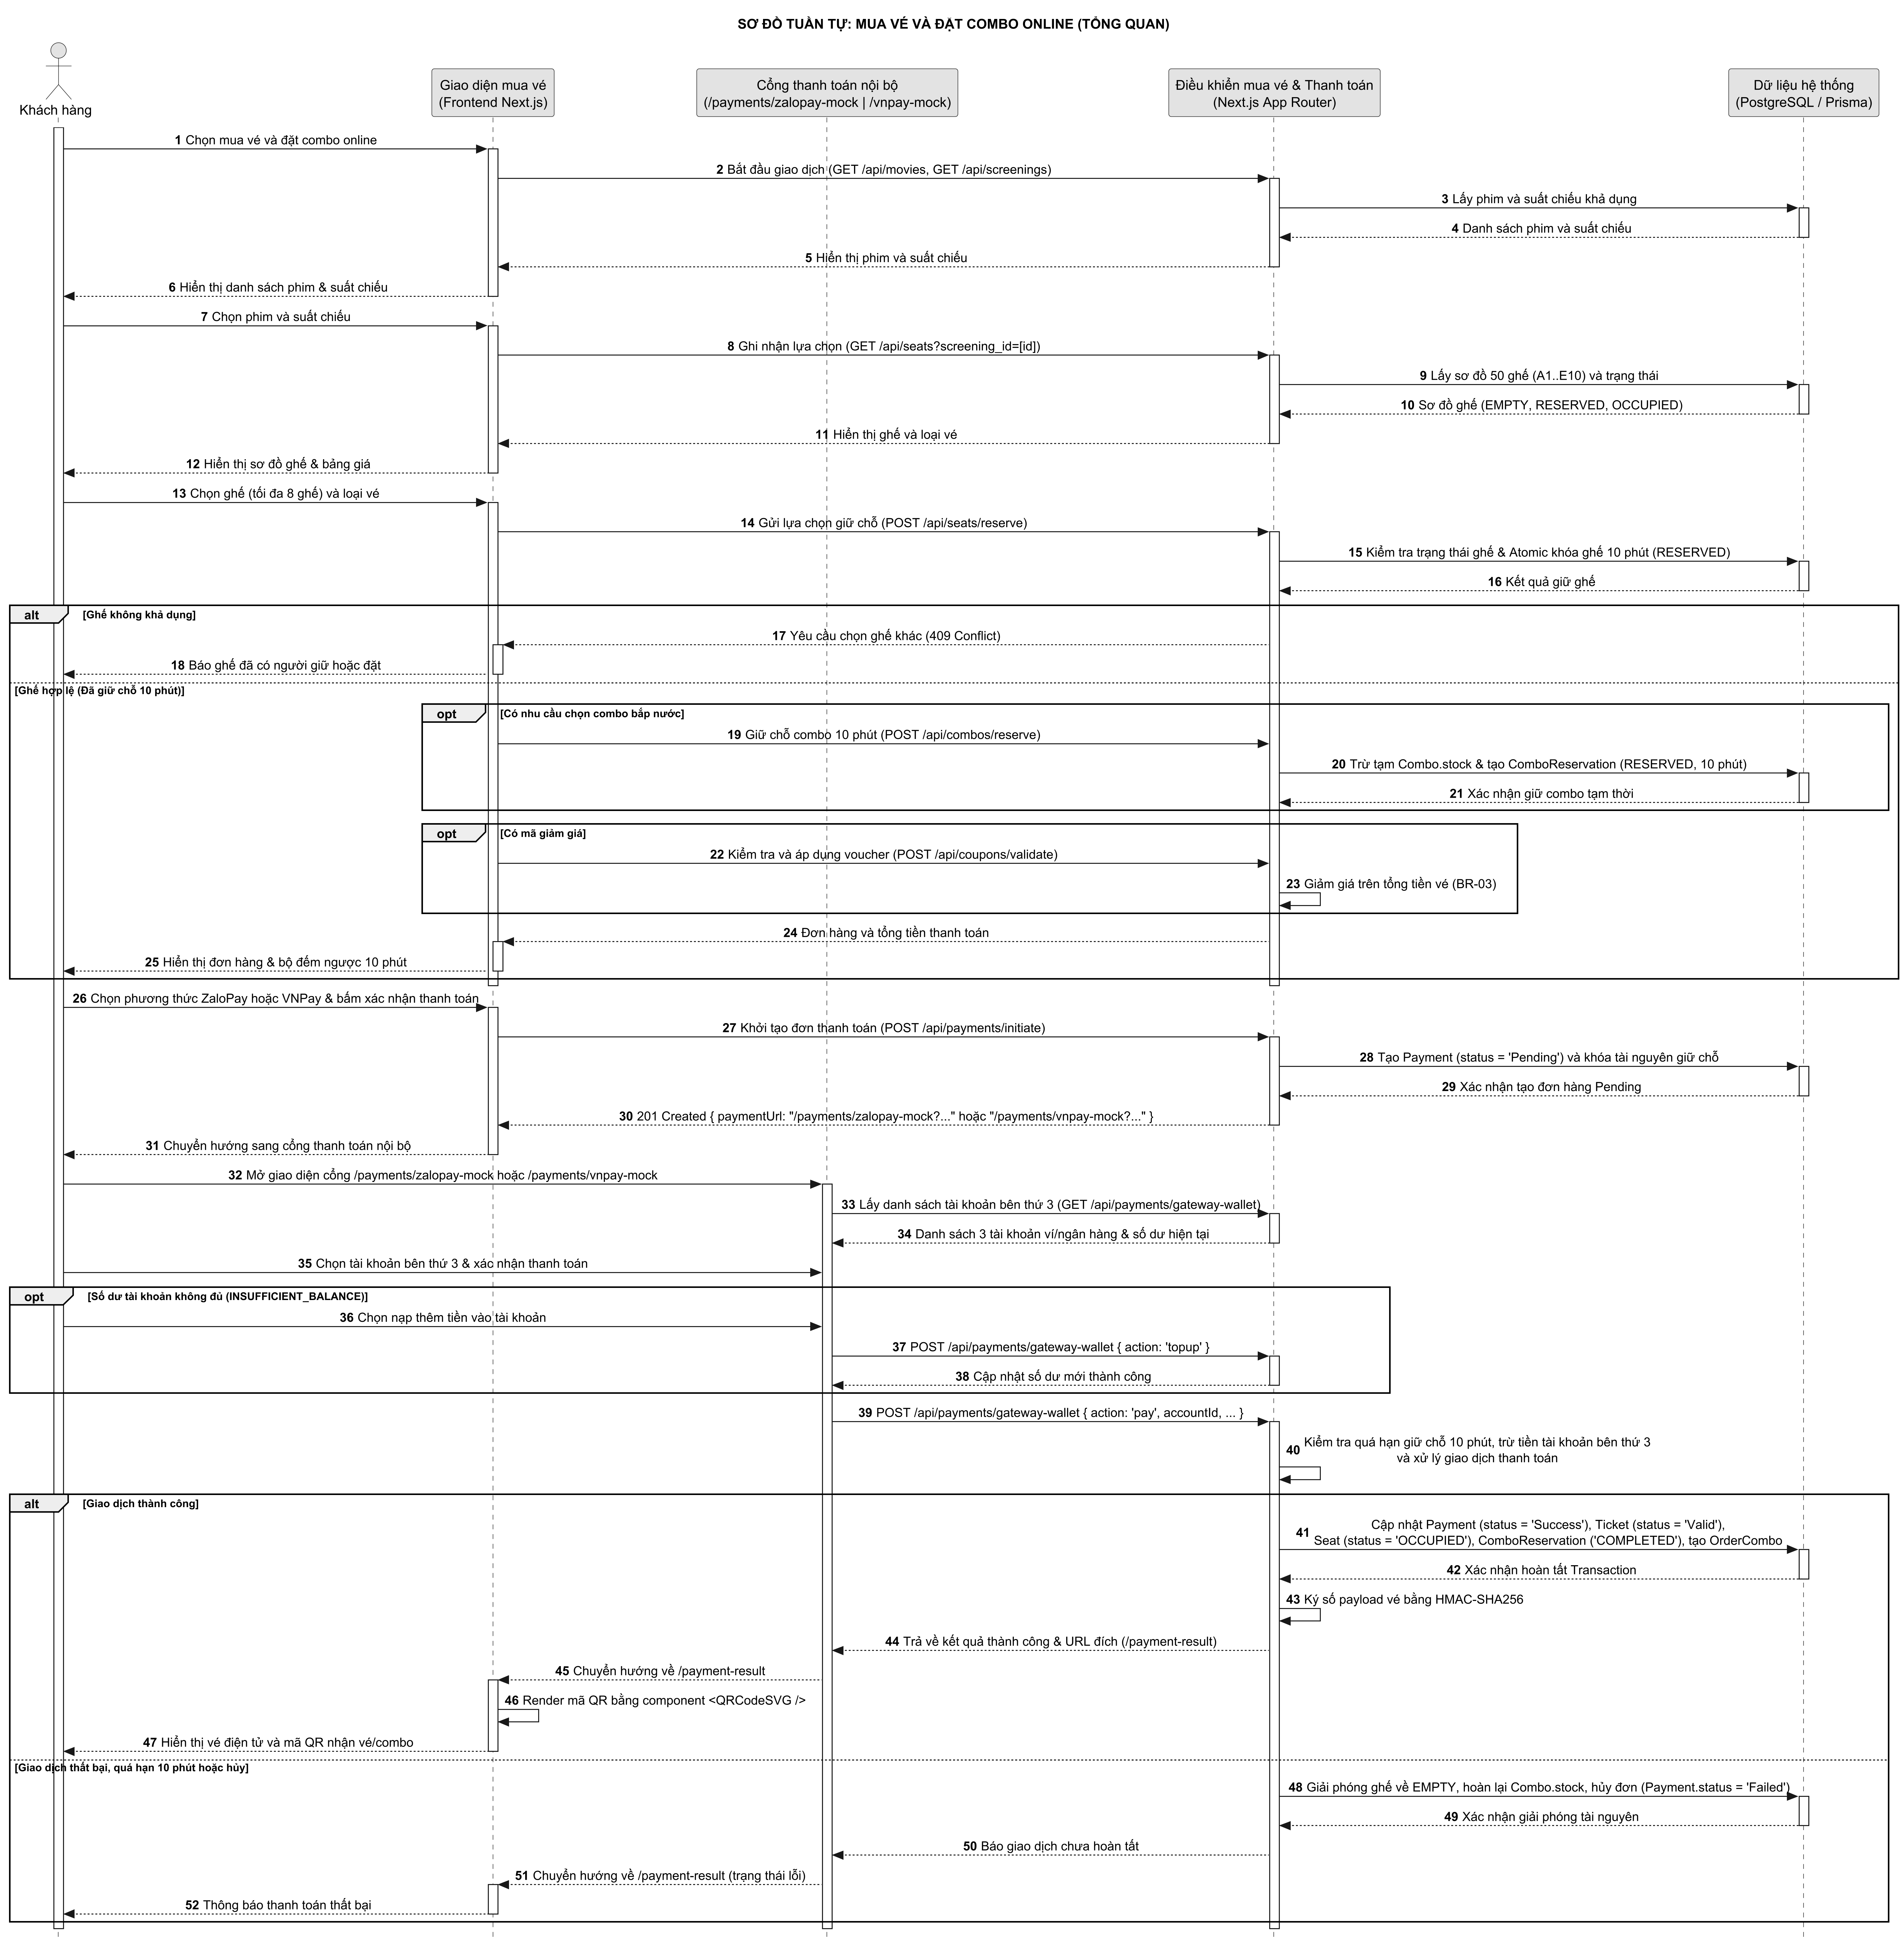
\includegraphics[width=\textwidth,height=0.80\textheight,keepaspectratio]{images/sequence/04_mua_ve_va_dat_combo_online_tong_quan.png}
  \caption{Sequence Diagram: SƠ ĐỒ TUẦN TỰ: MUA VÉ VÀ ĐẶT COMBO ONLINE (TỔNG QUAN)}
  \label{fig:seq_04}
\end{figure}

\subsection{SƠ ĐỒ TUẦN TỰ: XEM PHIM VÀ SUẤT CHIẾU}
\begin{figure}[H]
  \centering
  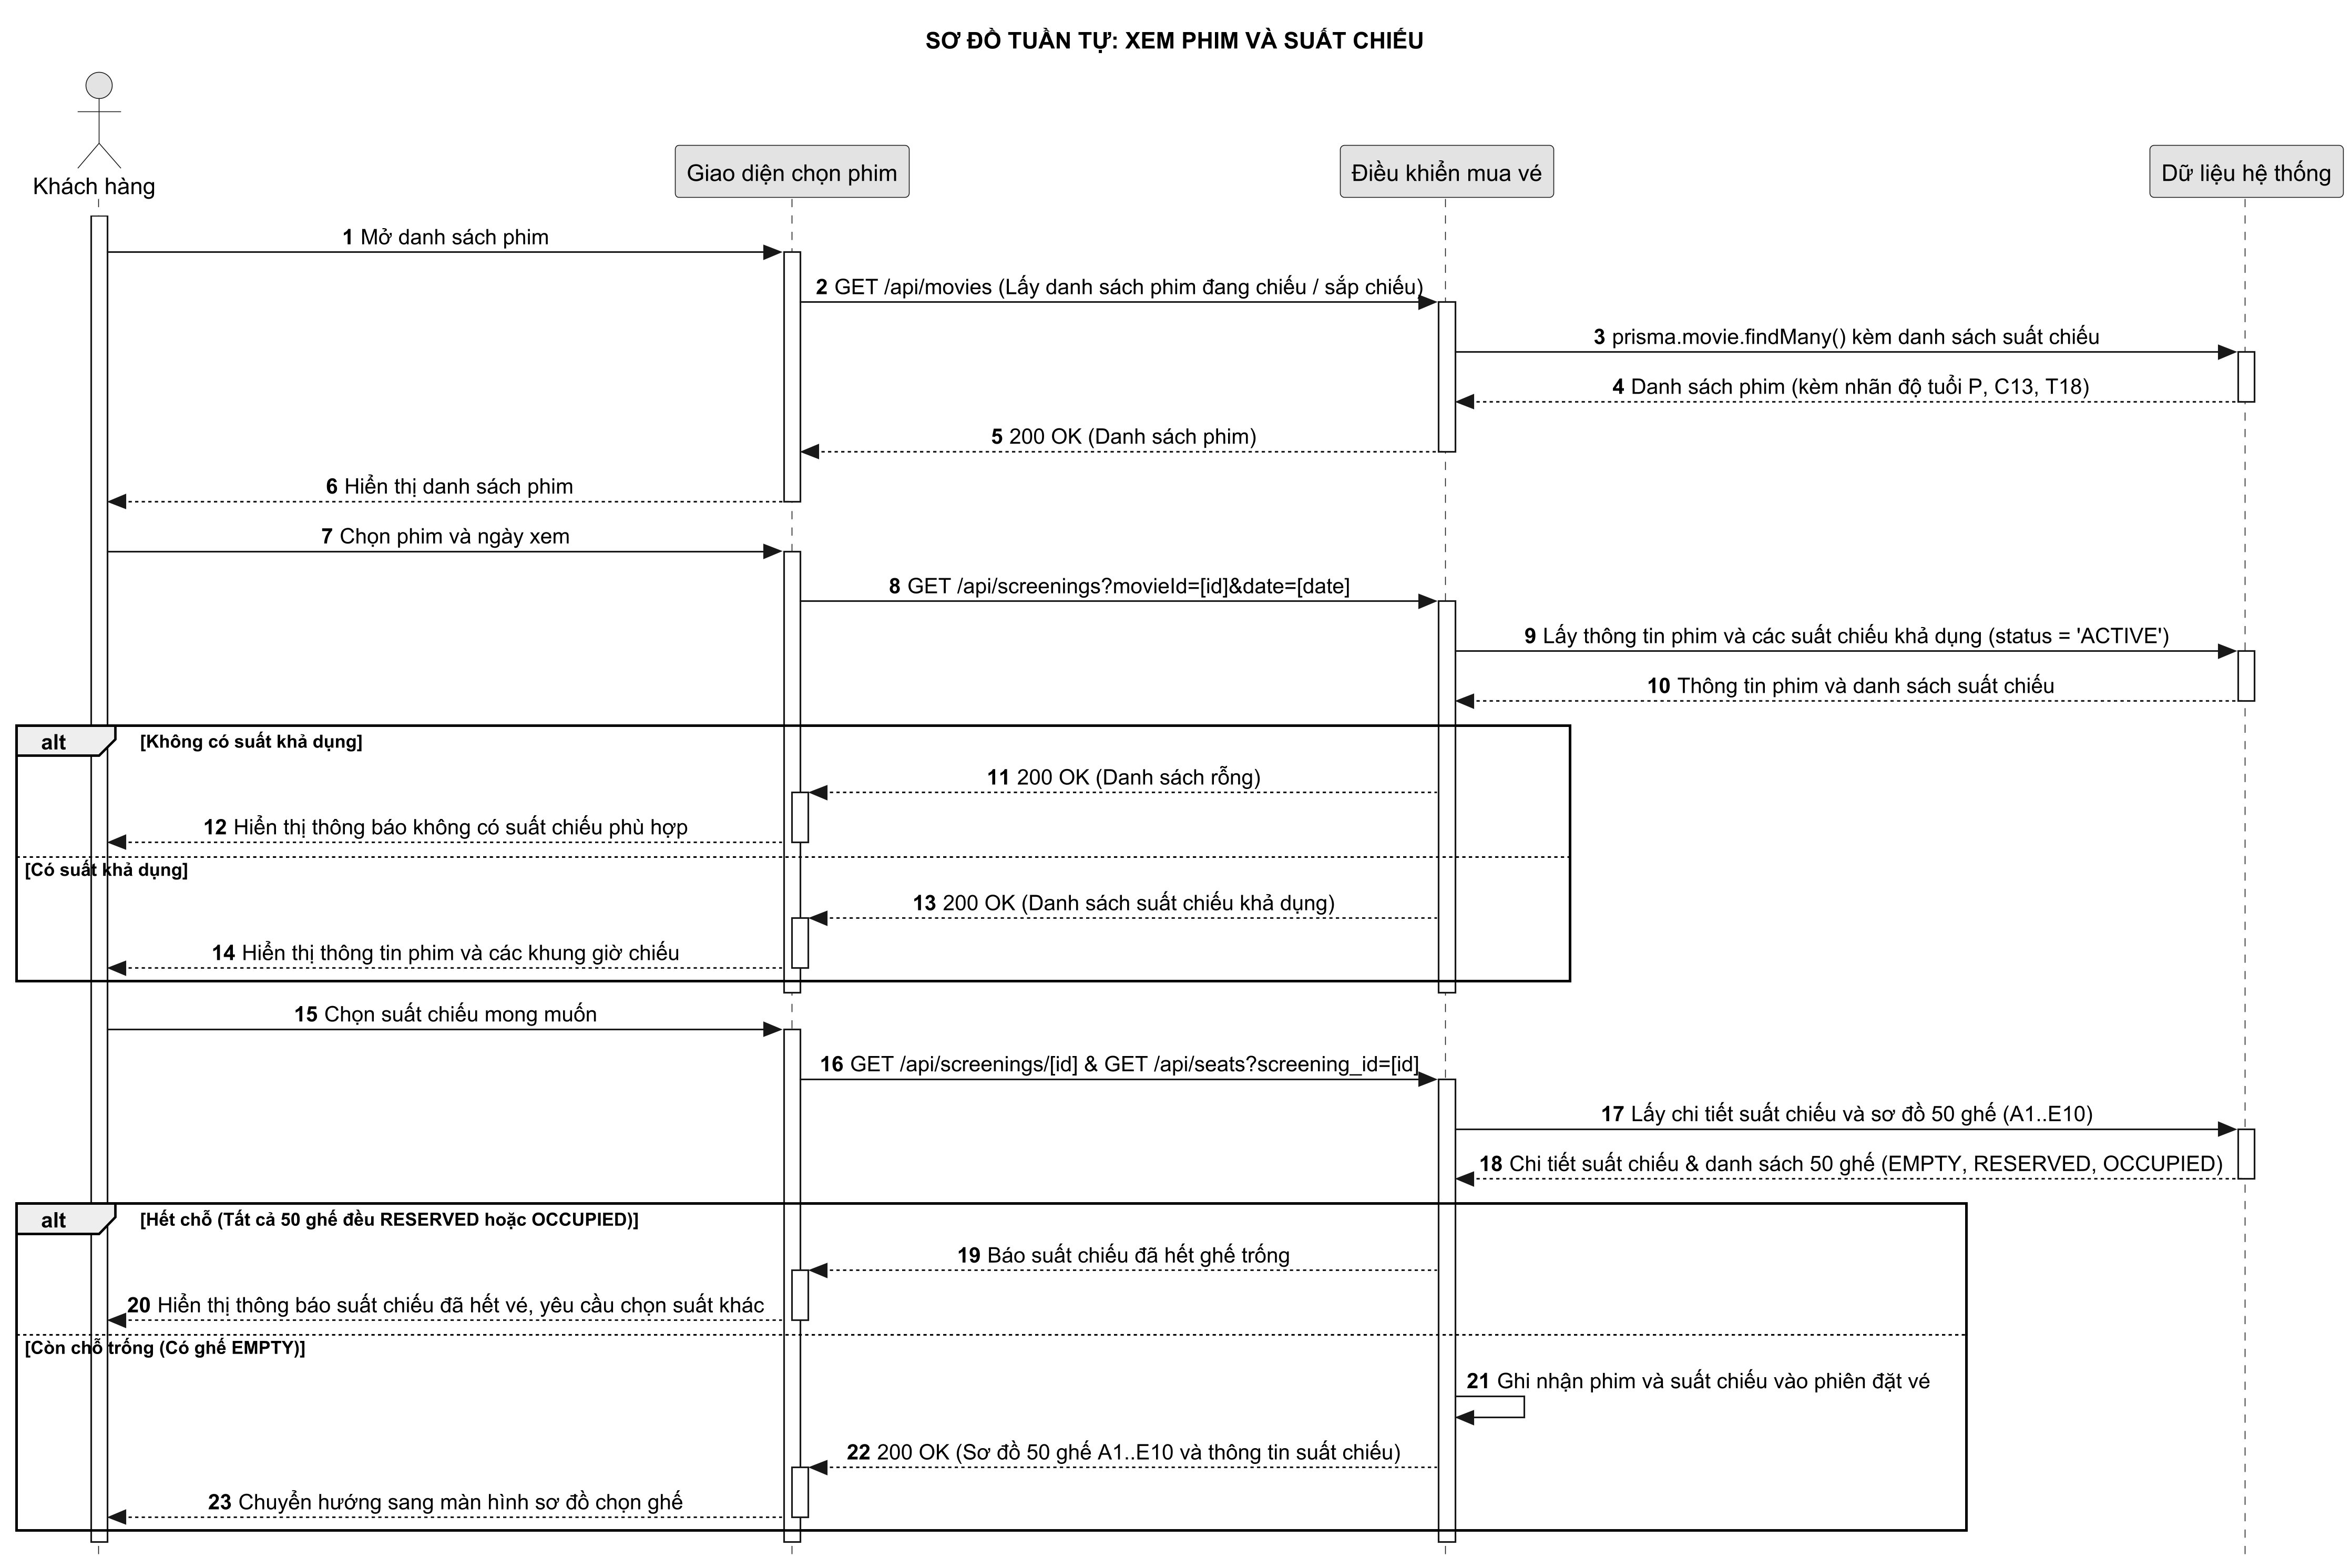
\includegraphics[width=\textwidth,height=0.80\textheight,keepaspectratio]{images/sequence/05_xem_phim_va_suat_chieu.png}
  \caption{Sequence Diagram: SƠ ĐỒ TUẦN TỰ: XEM PHIM VÀ SUẤT CHIẾU}
  \label{fig:seq_05}
\end{figure}

\subsection{SƠ ĐỒ TUẦN TỰ: CHỌN GHẾ VÀ GIỮ CHỖ TẠM THỜI}
\begin{figure}[H]
  \centering
  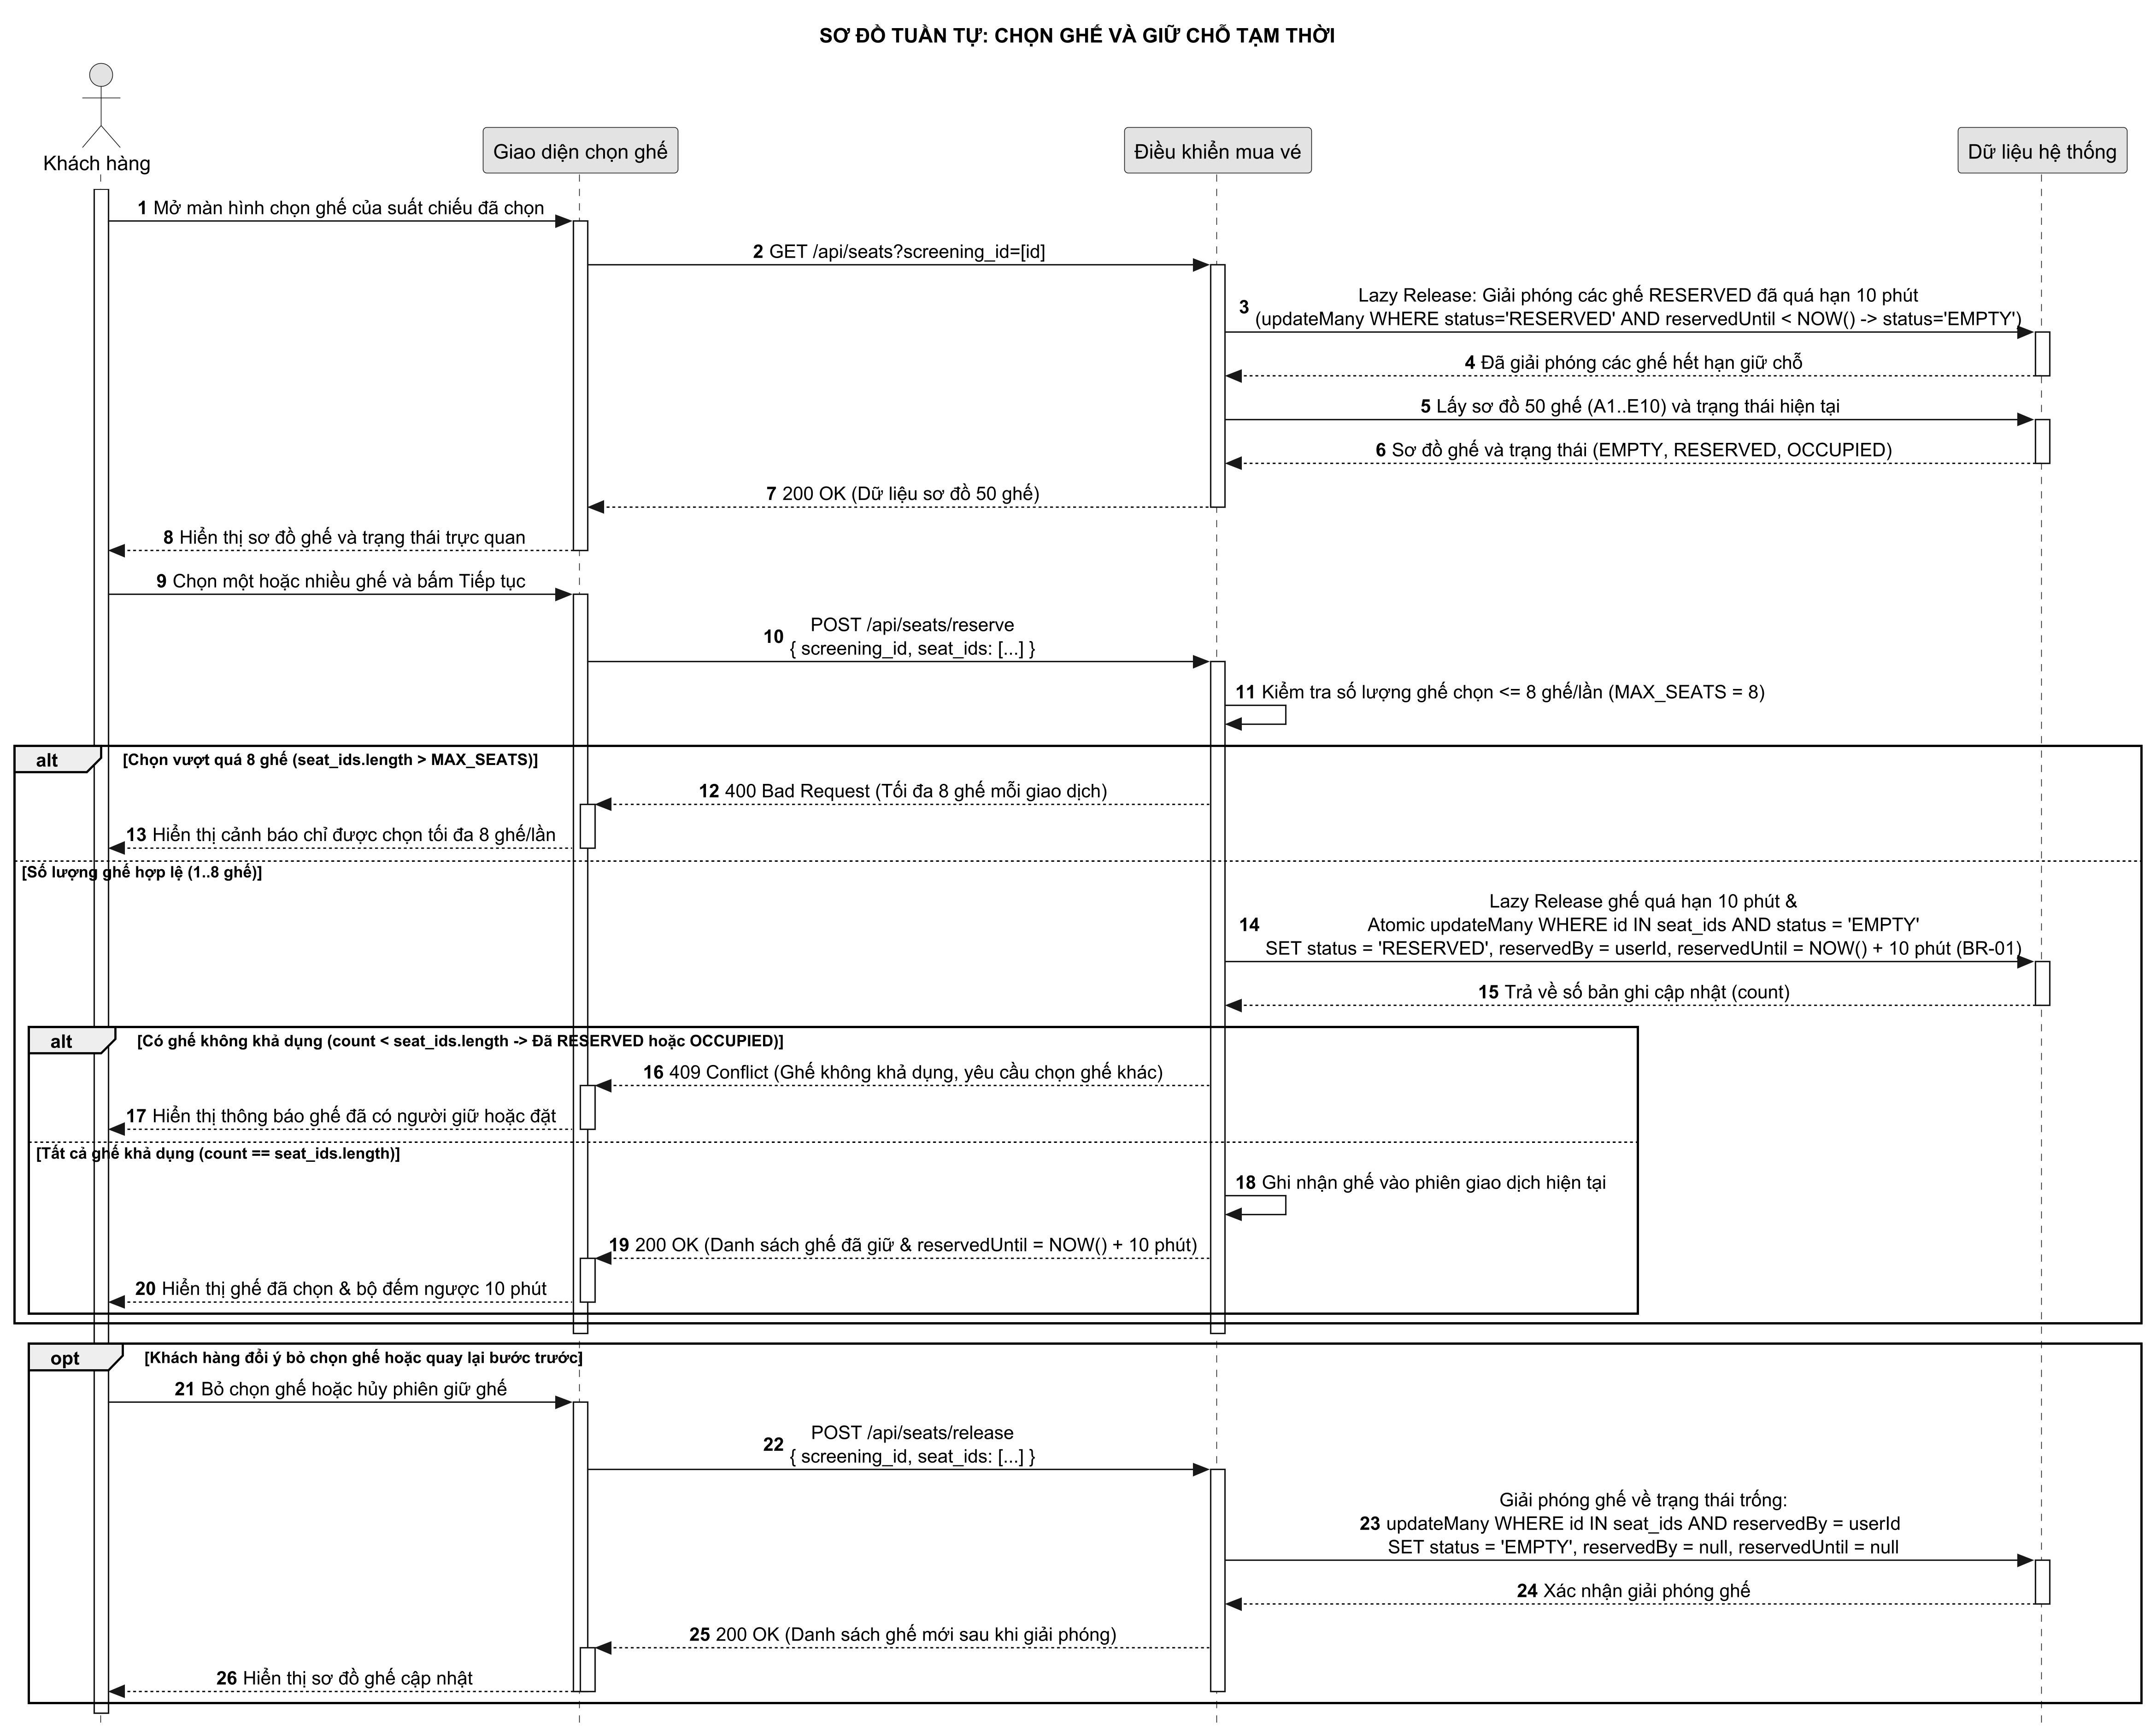
\includegraphics[width=\textwidth,height=0.80\textheight,keepaspectratio]{images/sequence/06_chon_ghe_va_giu_cho.png}
  \caption{Sequence Diagram: SƠ ĐỒ TUẦN TỰ: CHỌN GHẾ VÀ GIỮ CHỖ TẠM THỜI}
  \label{fig:seq_06}
\end{figure}

\subsection{SƠ ĐỒ TUẦN TỰ: CHỌN LOẠI VÉ}
\begin{figure}[H]
  \centering
  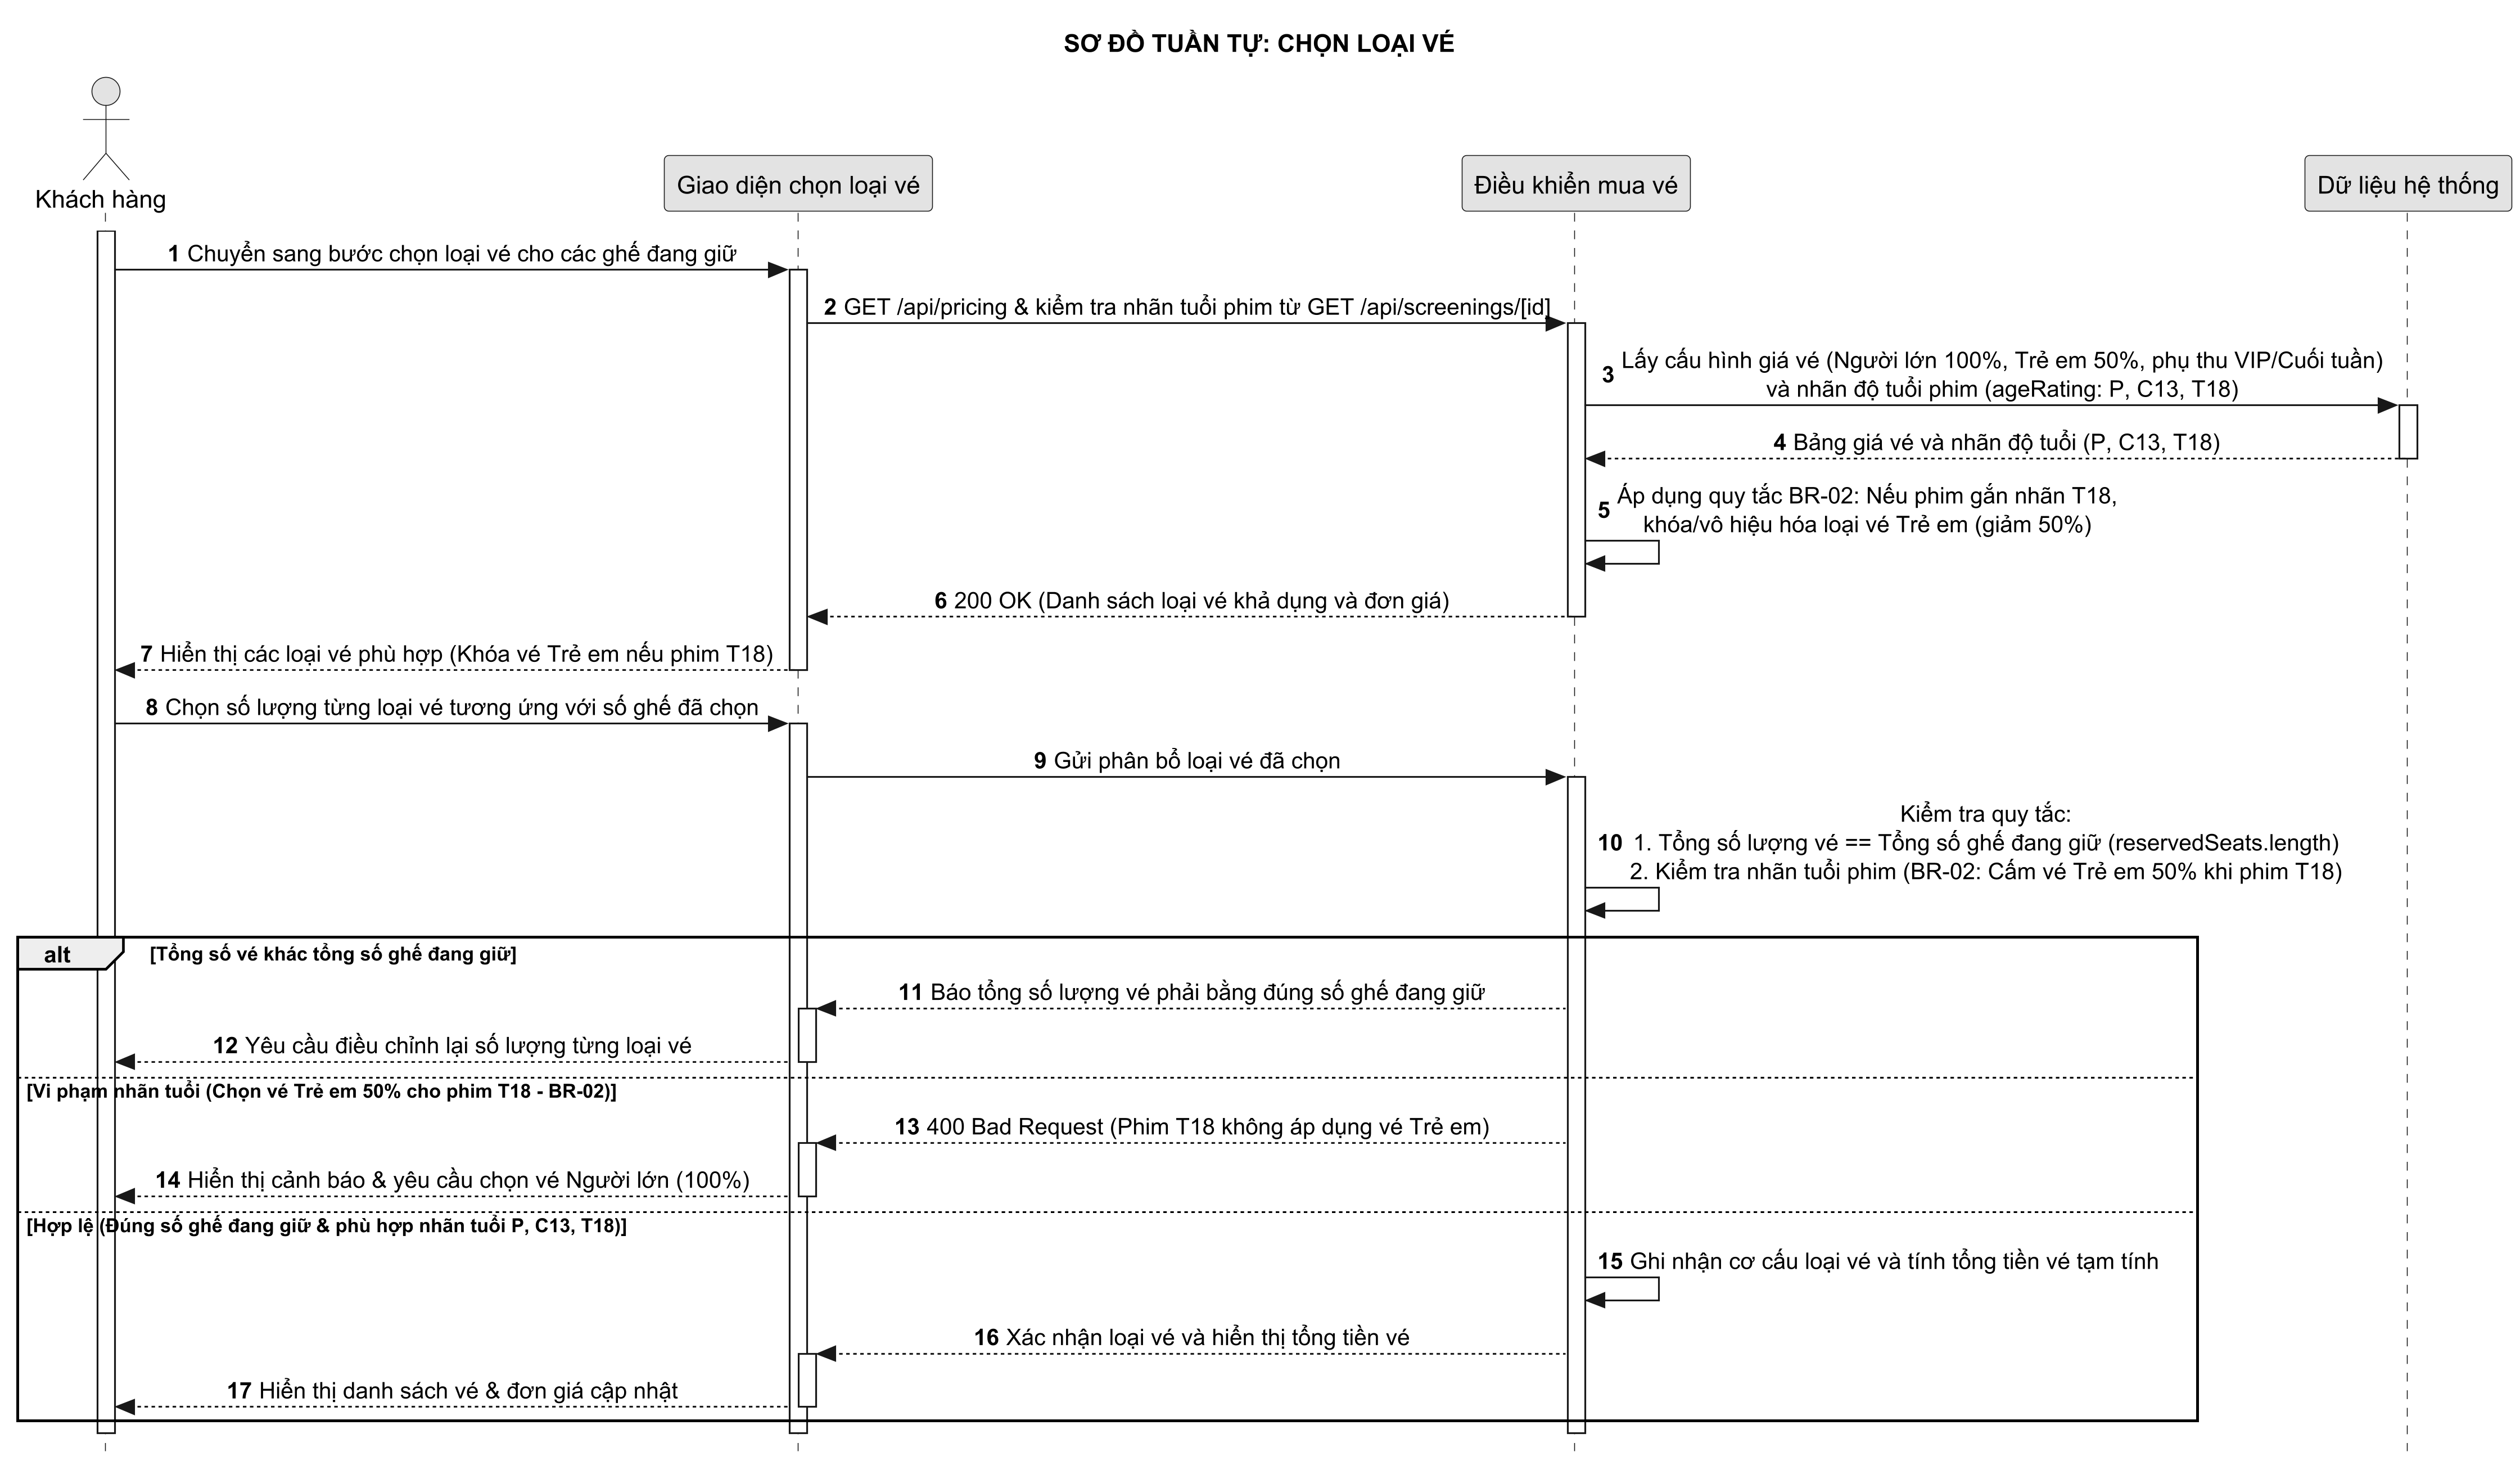
\includegraphics[width=\textwidth,height=0.80\textheight,keepaspectratio]{images/sequence/07_chon_loai_ve.png}
  \caption{Sequence Diagram: SƠ ĐỒ TUẦN TỰ: CHỌN LOẠI VÉ}
  \label{fig:seq_07}
\end{figure}

\subsection{SƠ ĐỒ TUẦN TỰ: THÊM COMBO VÀO ĐƠN HÀNG}
\begin{figure}[H]
  \centering
  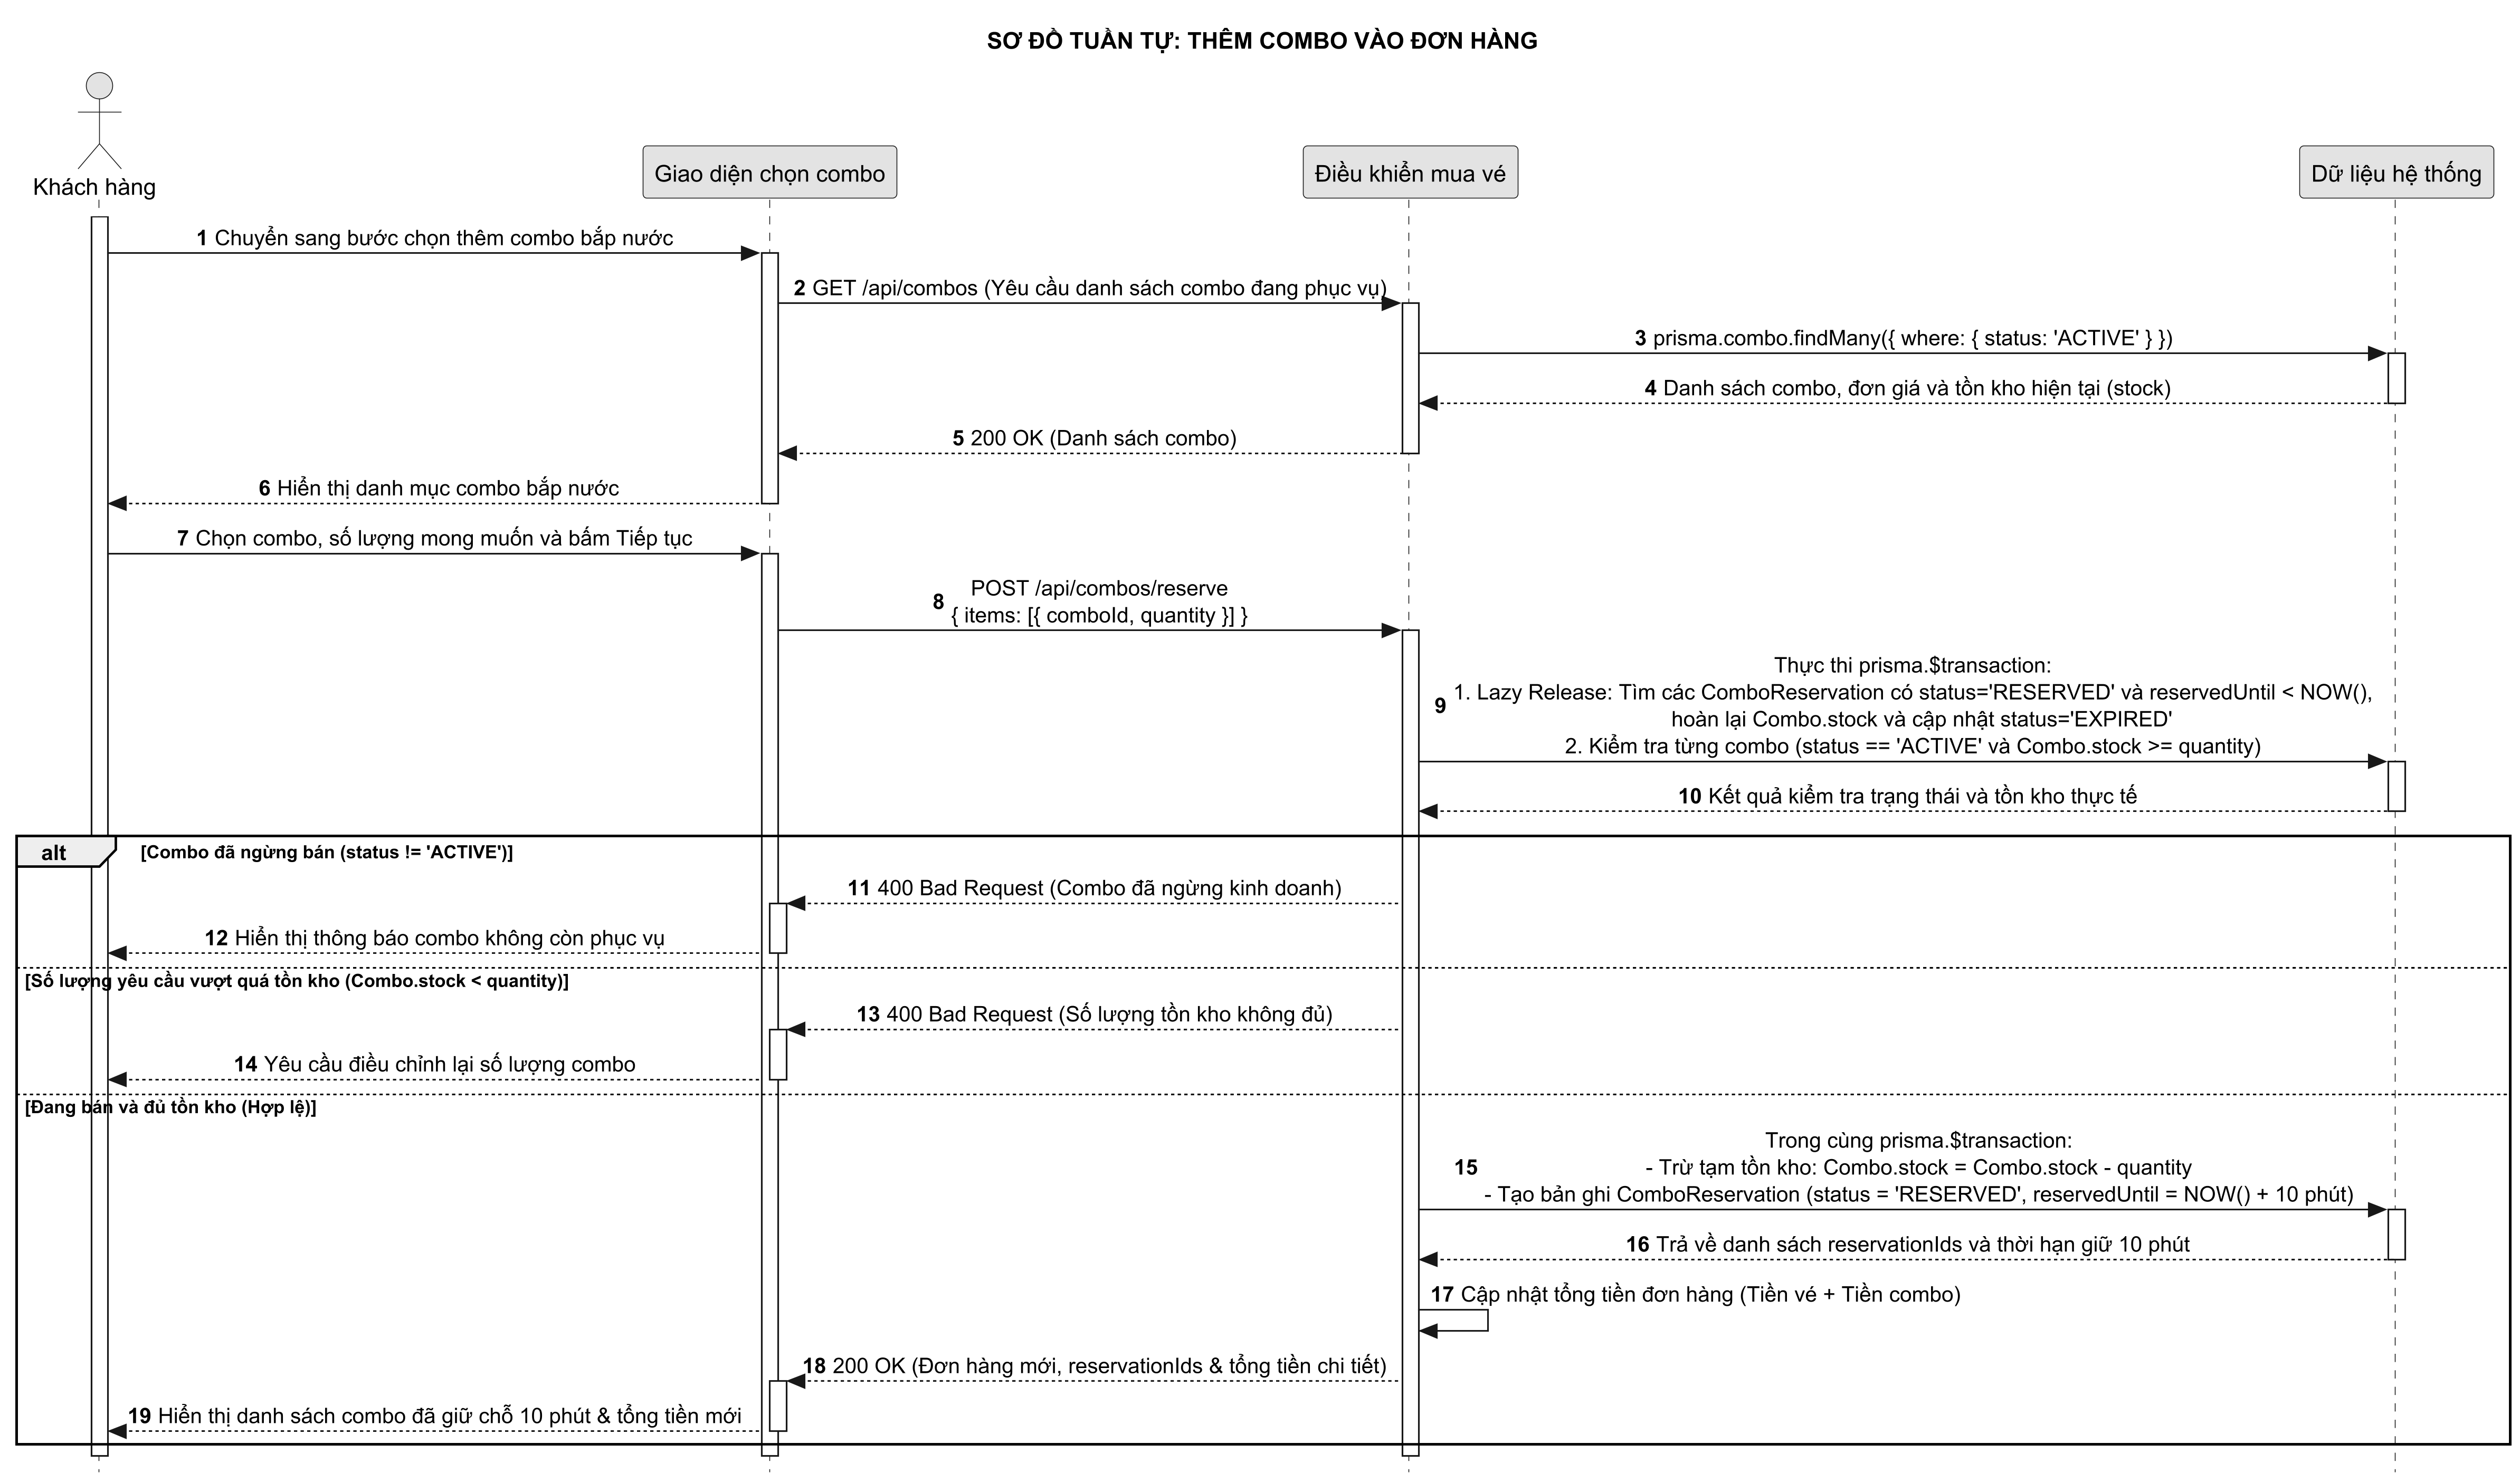
\includegraphics[width=\textwidth,height=0.80\textheight,keepaspectratio]{images/sequence/08_them_combo_vao_don_hang.png}
  \caption{Sequence Diagram: SƠ ĐỒ TUẦN TỰ: THÊM COMBO VÀO ĐƠN HÀNG}
  \label{fig:seq_08}
\end{figure}

\subsection{SƠ ĐỒ TUẦN TỰ: ÁP DỤNG VOUCHER KHUYẾN MÃI}
\begin{figure}[H]
  \centering
  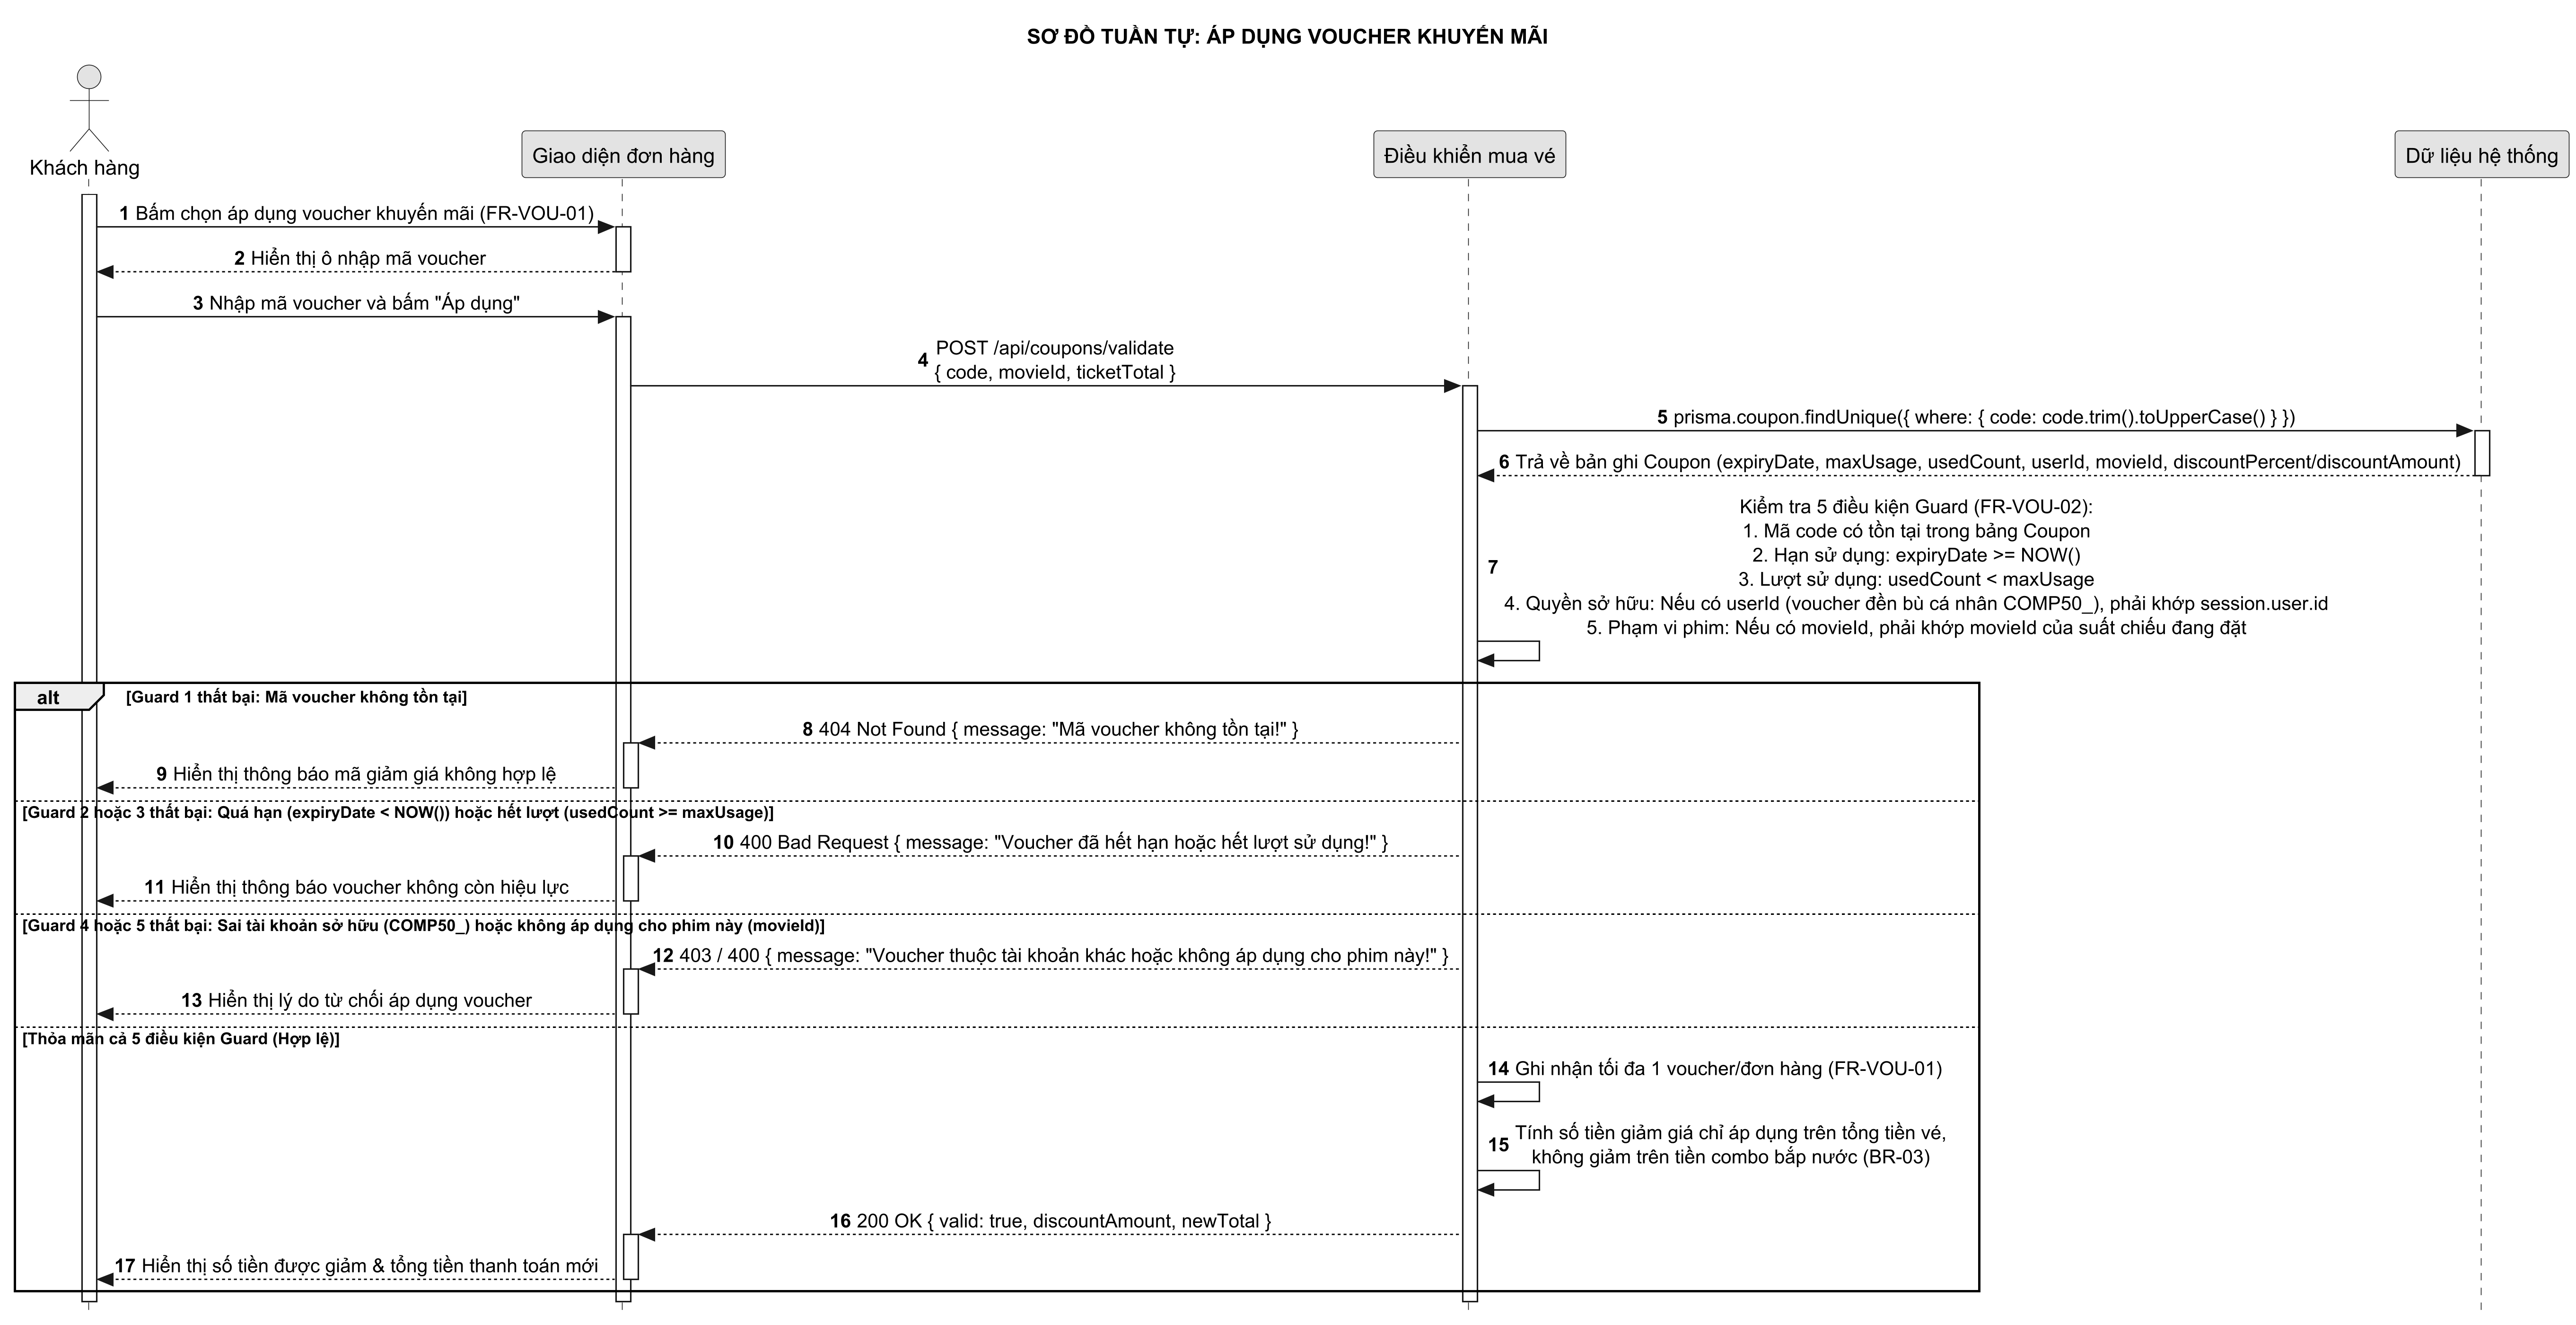
\includegraphics[width=\textwidth,height=0.80\textheight,keepaspectratio]{images/sequence/09_ap_dung_voucher.png}
  \caption{Sequence Diagram: SƠ ĐỒ TUẦN TỰ: ÁP DỤNG VOUCHER KHUYẾN MÃI}
  \label{fig:seq_09}
\end{figure}

\subsection{SƠ ĐỒ TUẦN TỰ: XỬ LÝ THANH TOÁN ONLINE QUA CỔNG NỘI BỘ (ZALOPAY \& VNPAY GATEWAY)}
\begin{figure}[H]
  \centering
  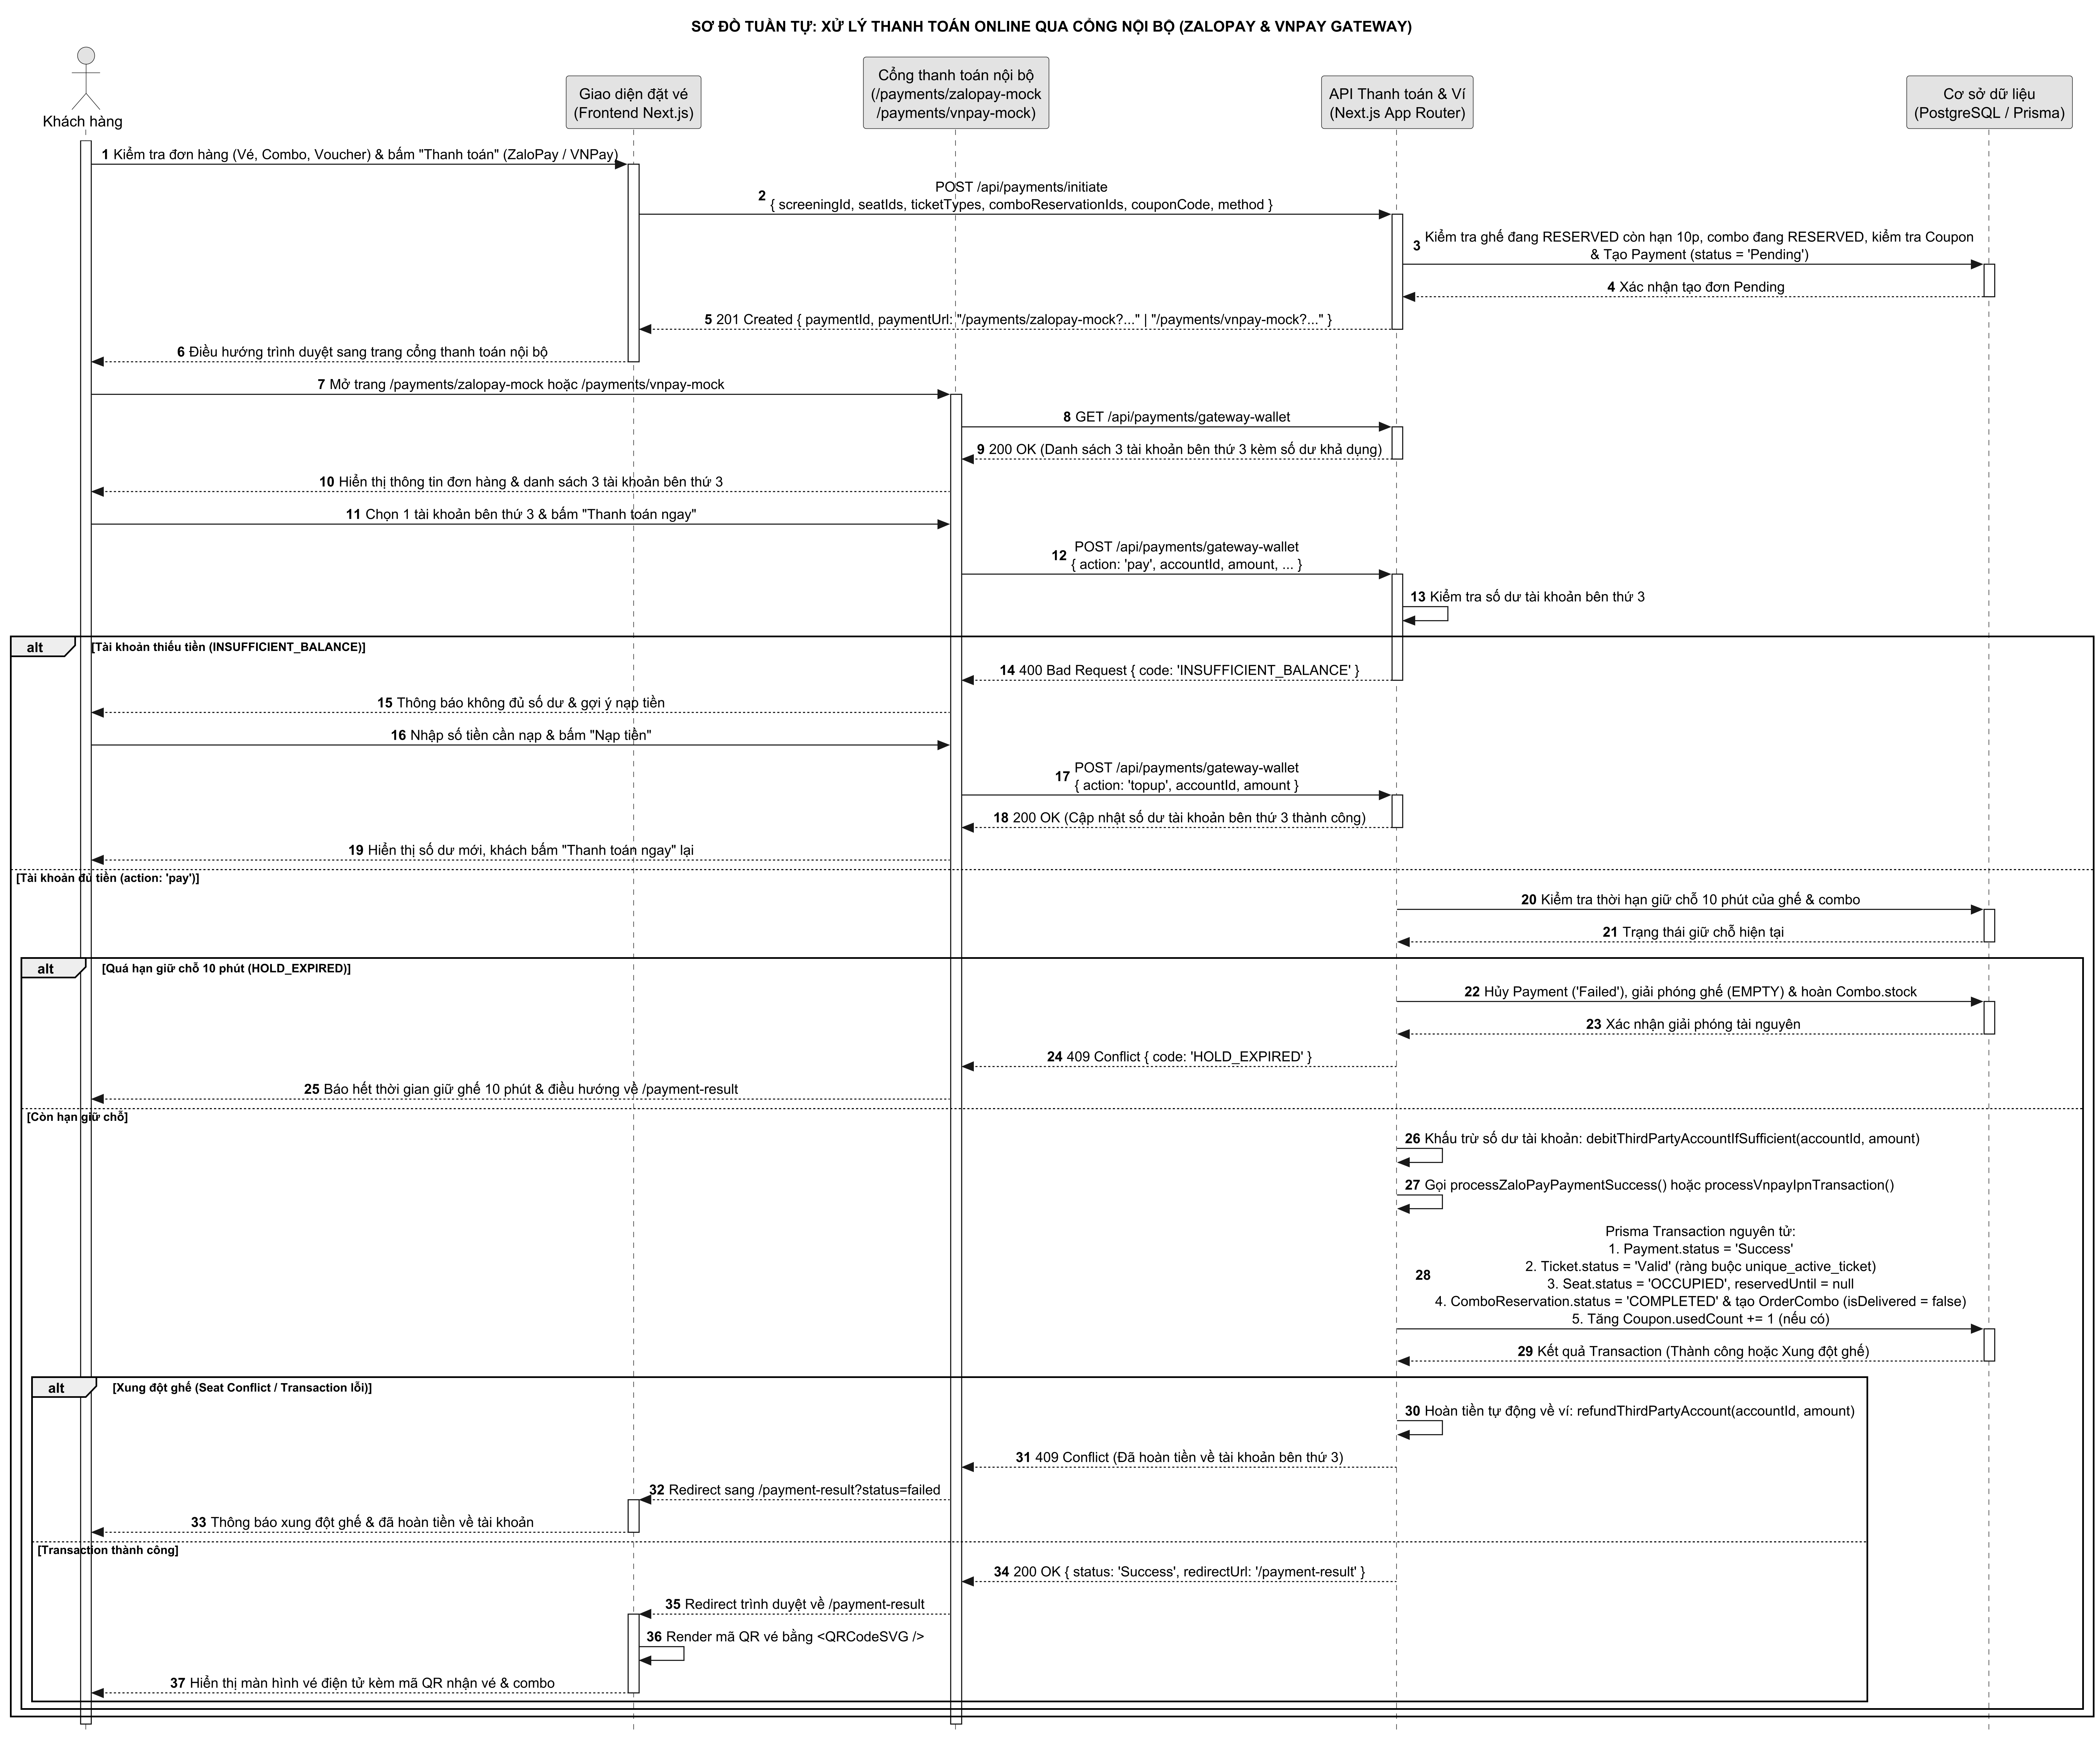
\includegraphics[width=\textwidth,height=0.80\textheight,keepaspectratio]{images/sequence/10_thanh_toan_online.png}
  \caption{Sequence Diagram: SƠ ĐỒ TUẦN TỰ: XỬ LÝ THANH TOÁN ONLINE QUA CỔNG NỘI BỘ (ZALOPAY \& VNPAY GATEWAY)}
  \label{fig:seq_10}
\end{figure}

\subsection{SƠ ĐỒ TUẦN TỰ: THANH TOÁN ZALOPAY \& VNPAY GATEWAY (TÀI KHOẢN BÊN THỨ 3 \& KIỂM TRA SỐ DƯ)}
\begin{figure}[H]
  \centering
  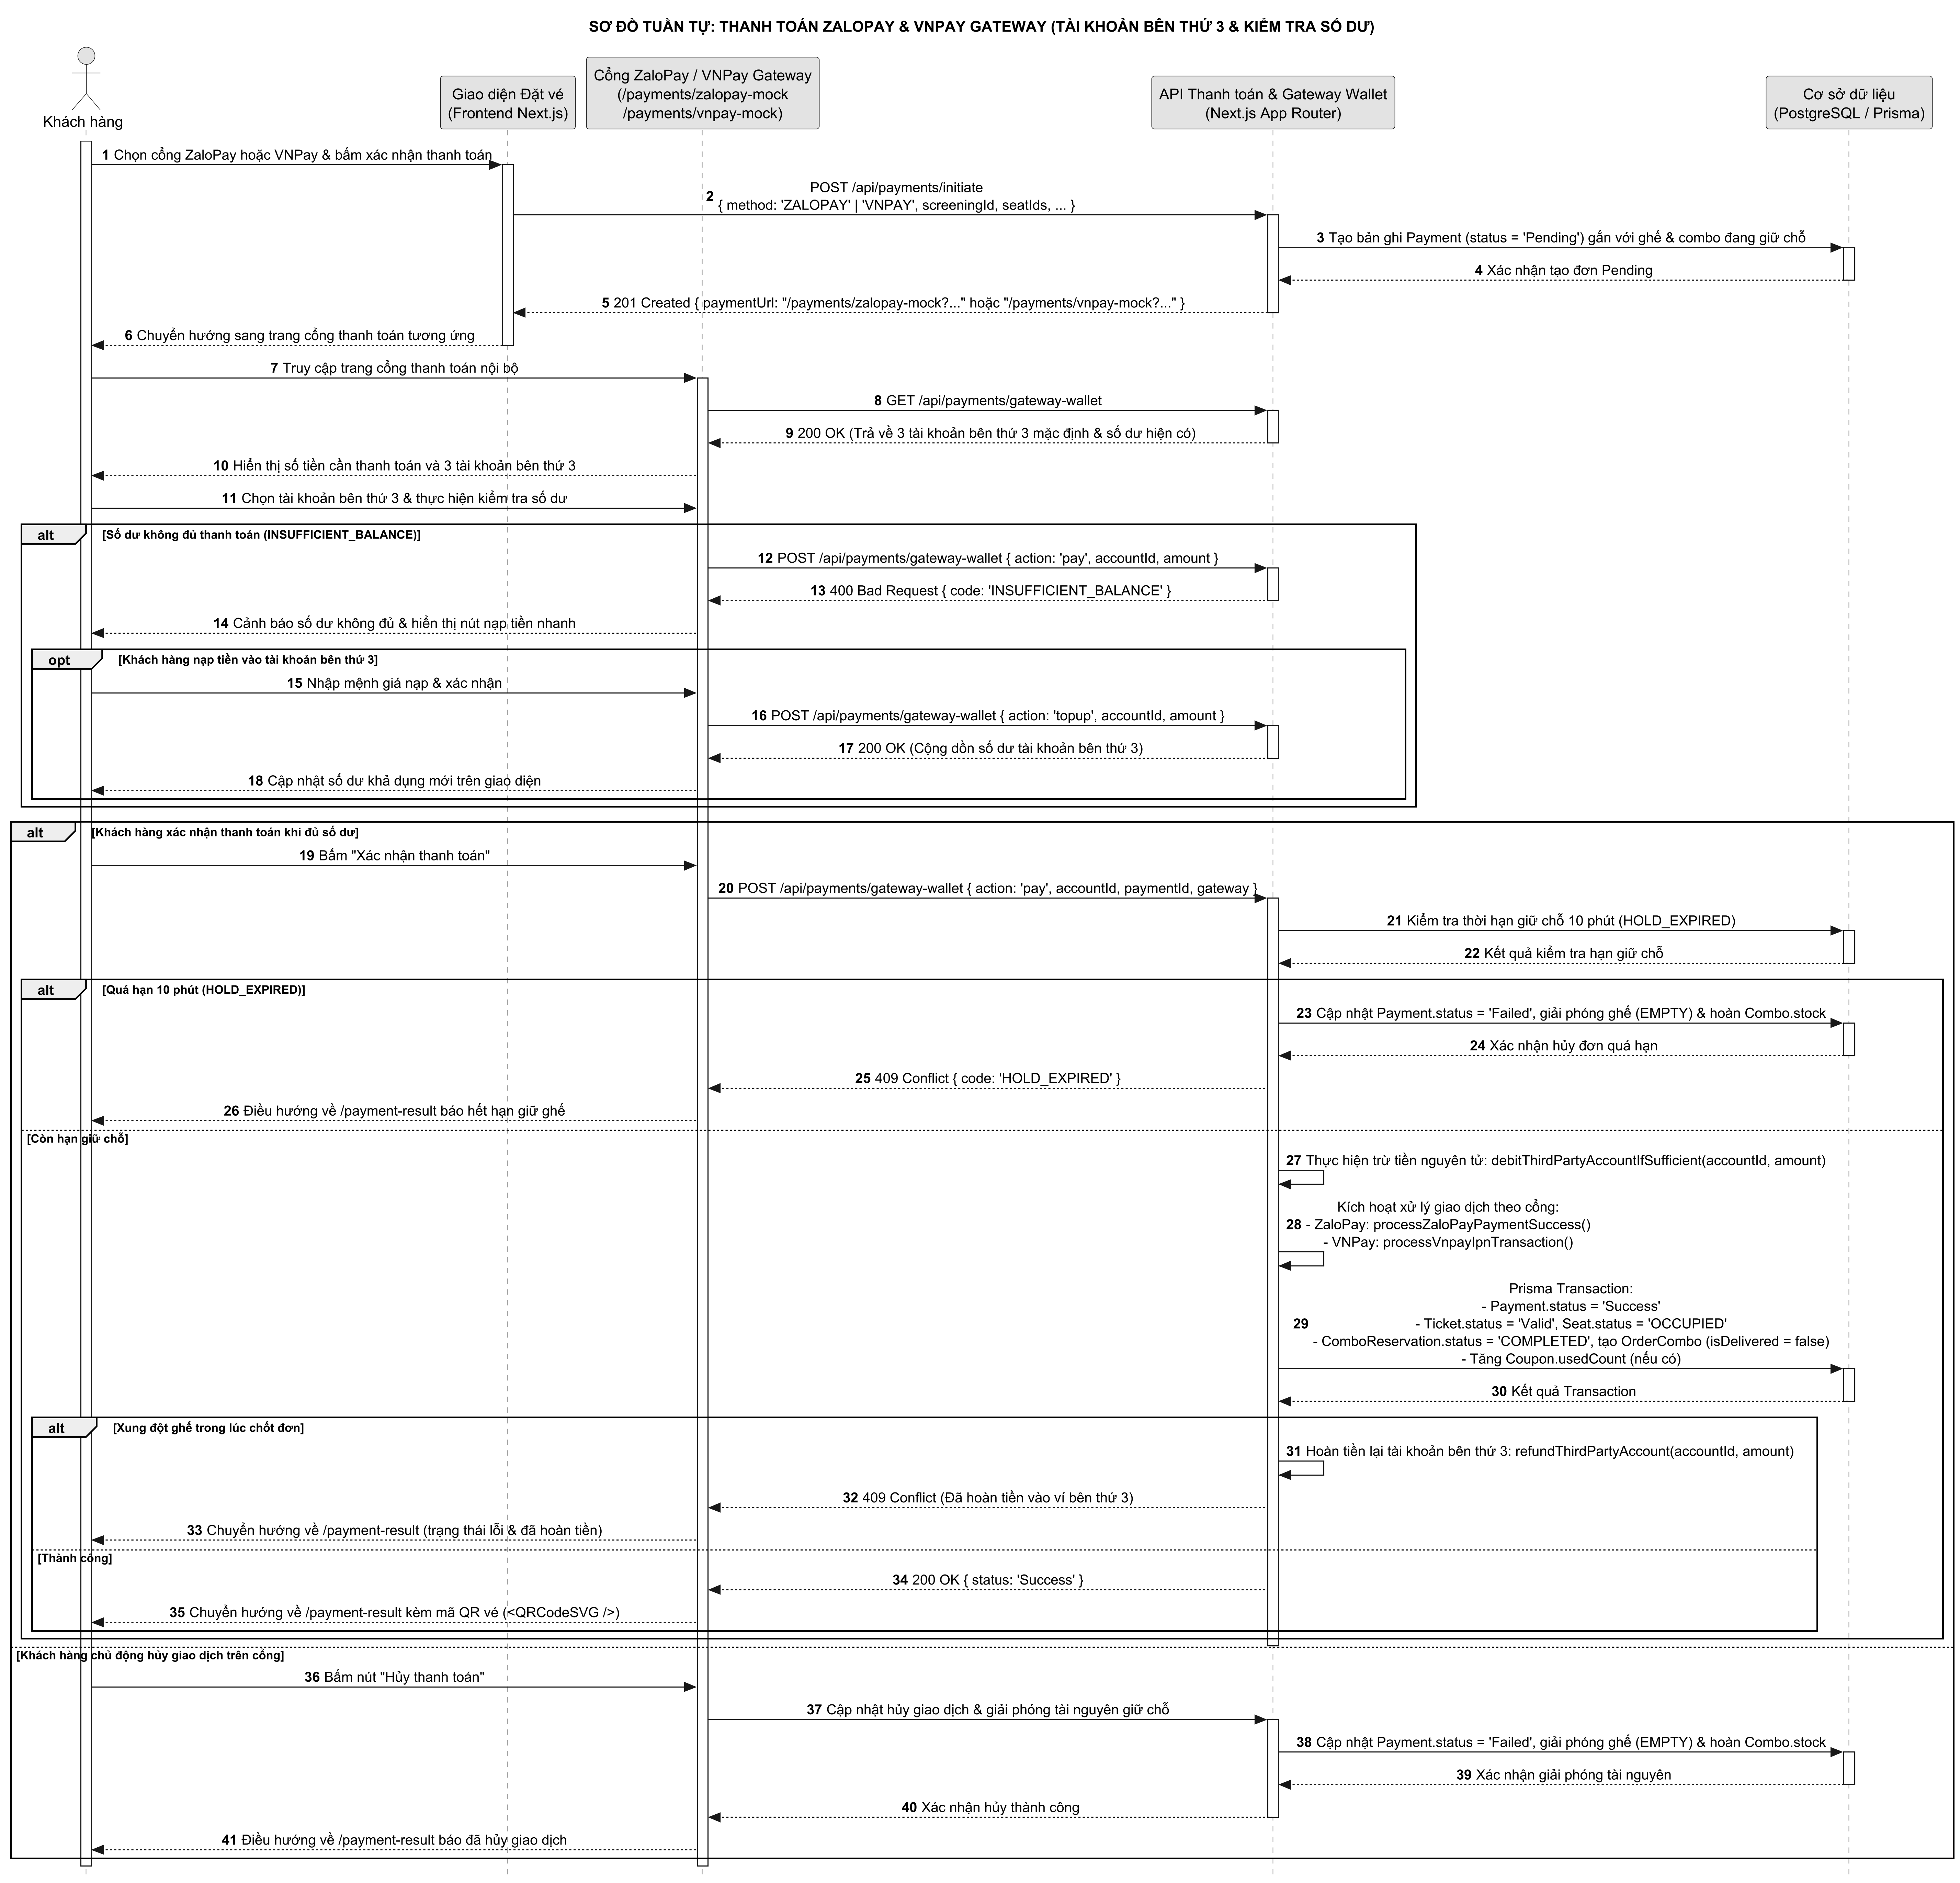
\includegraphics[width=\textwidth,height=0.80\textheight,keepaspectratio]{images/sequence/11_thanh_toan_vnpay_momo.png}
  \caption{Sequence Diagram: SƠ ĐỒ TUẦN TỰ: THANH TOÁN ZALOPAY \& VNPAY GATEWAY (TÀI KHOẢN BÊN THỨ 3 \& KIỂM TRA SỐ DƯ)}
  \label{fig:seq_11}
\end{figure}

\subsection{SƠ ĐỒ TUẦN TỰ: BÁN VÉ TẠI QUẦY POS (IN-PERSON TICKET SALES)}
\begin{figure}[H]
  \centering
  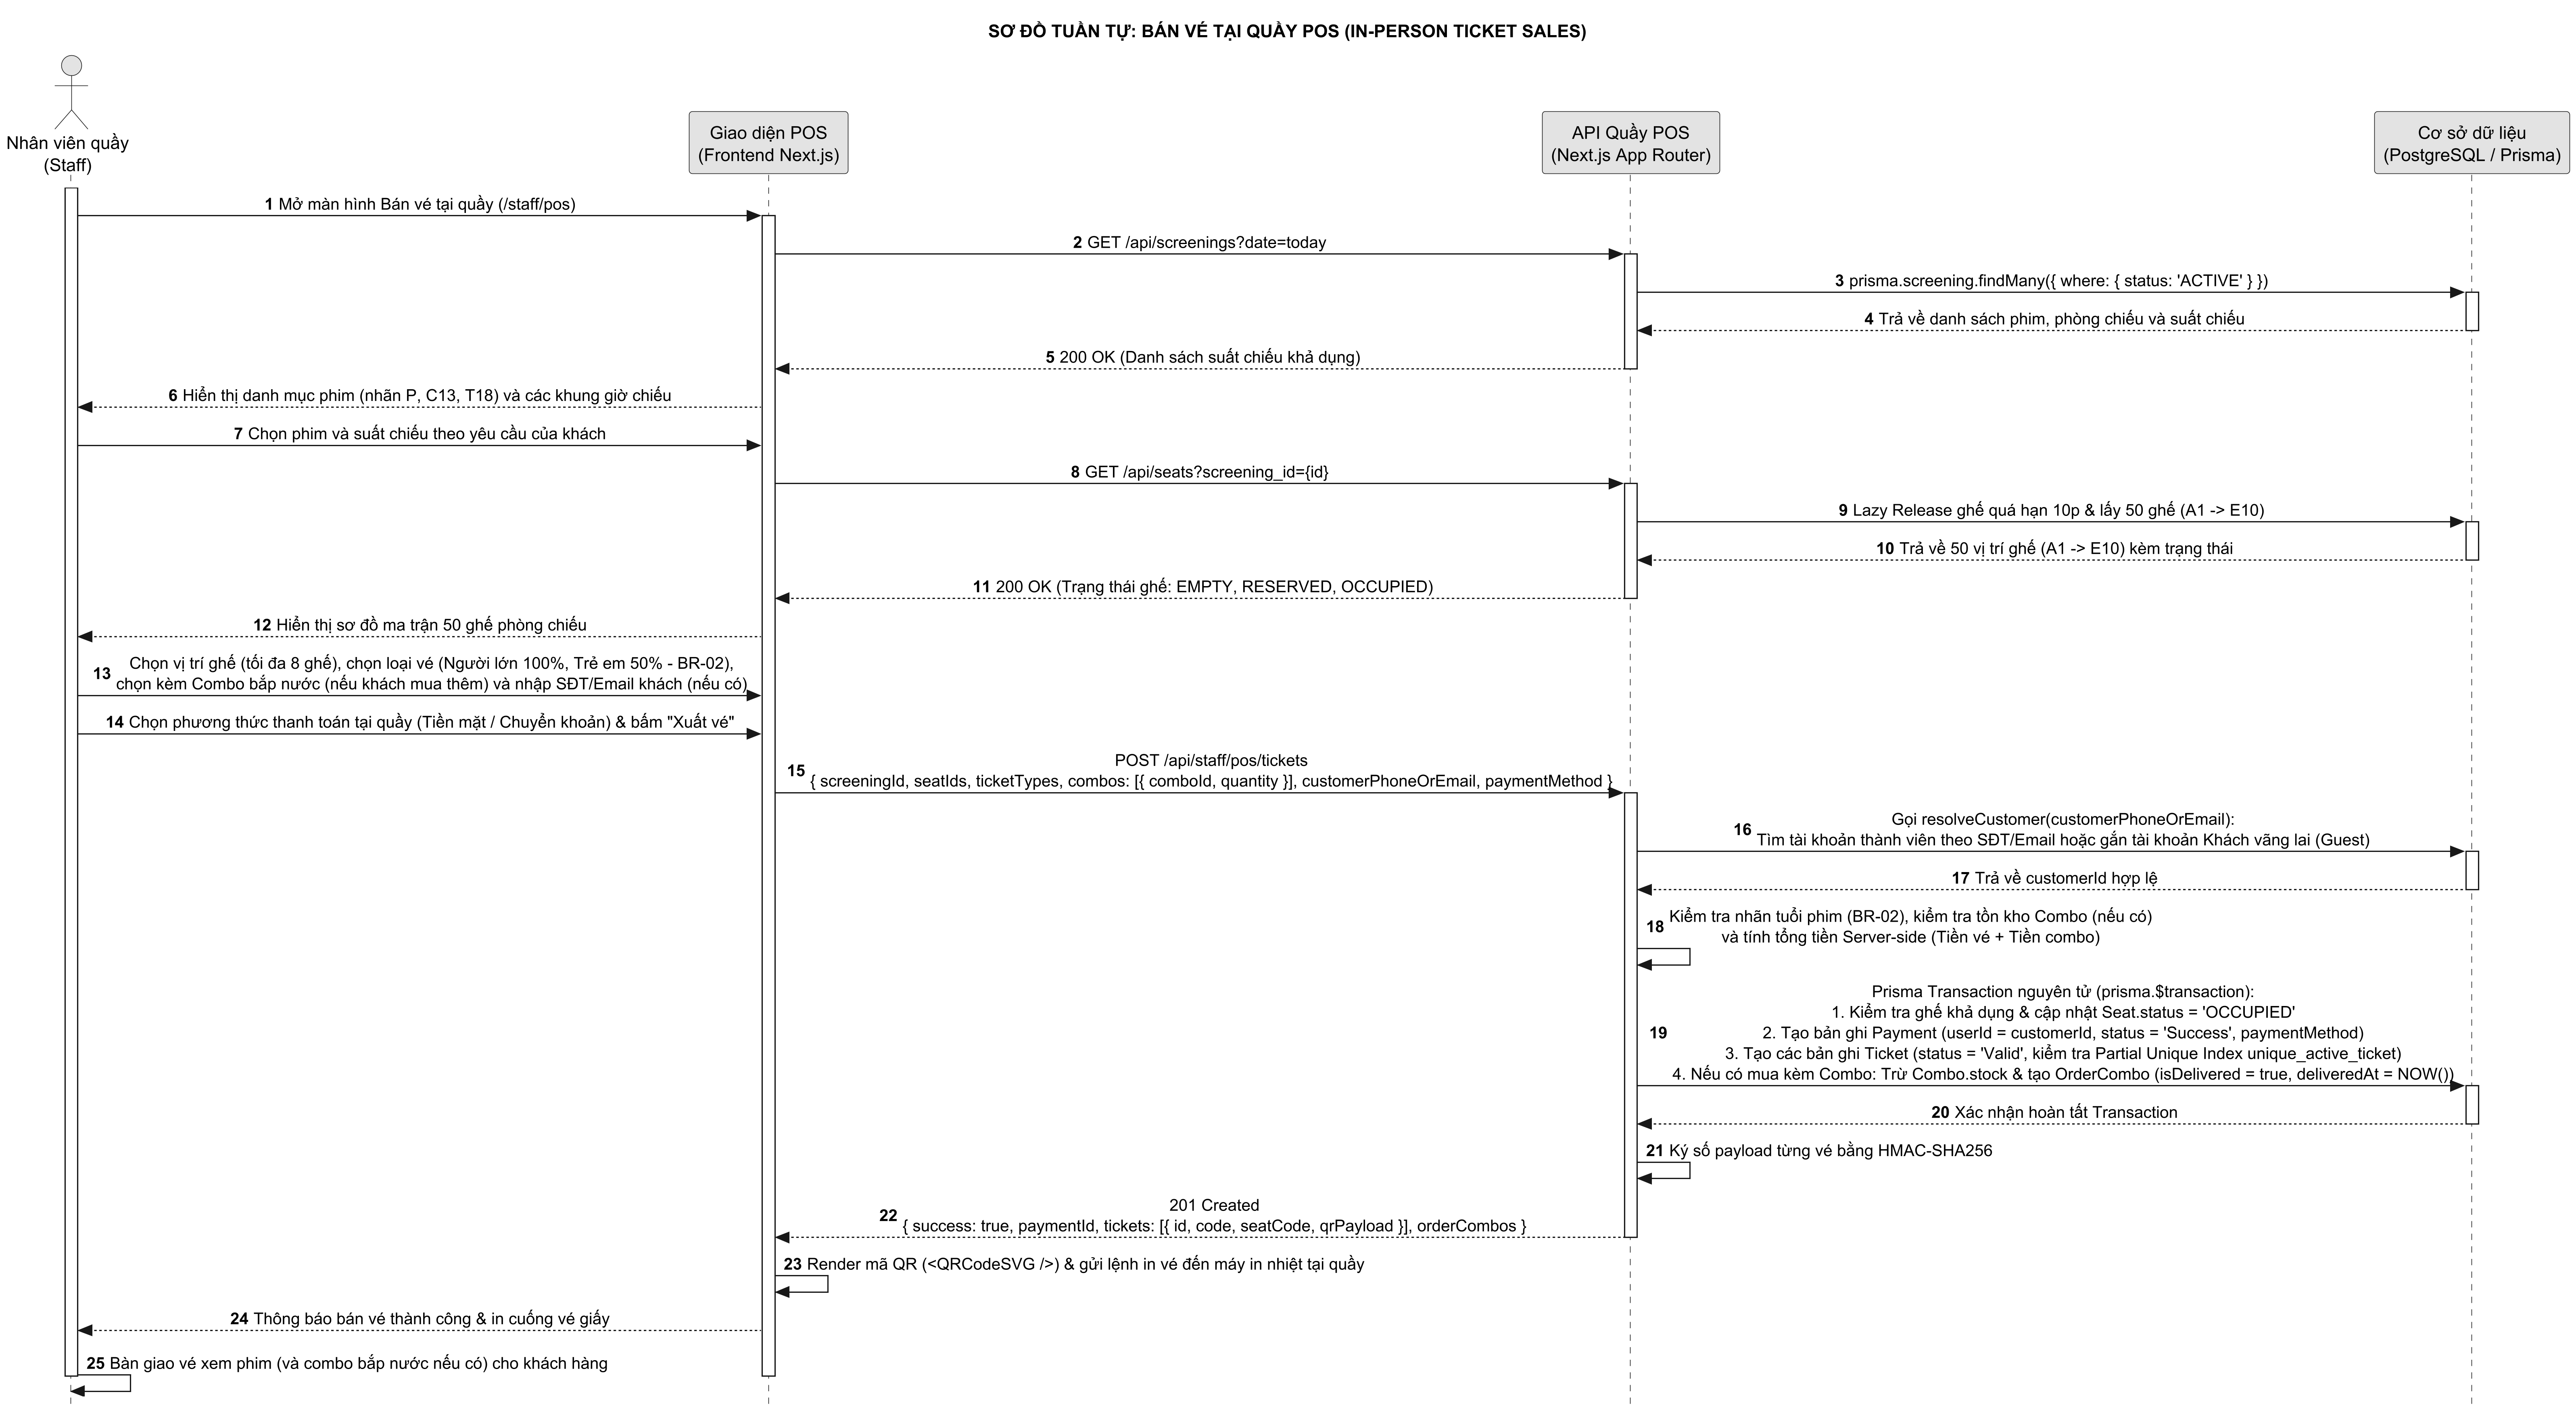
\includegraphics[width=\textwidth,height=0.80\textheight,keepaspectratio]{images/sequence/12_ban_ve_tai_quay_pos.png}
  \caption{Sequence Diagram: SƠ ĐỒ TUẦN TỰ: BÁN VÉ TẠI QUẦY POS (IN-PERSON TICKET SALES)}
  \label{fig:seq_12}
\end{figure}

\subsection{SƠ ĐỒ TUẦN TỰ: BÁN COMBO BẮP NƯỚC LẺ TẠI QUẦY POS (POS STANDALONE COMBO SALES)}
\begin{figure}[H]
  \centering
  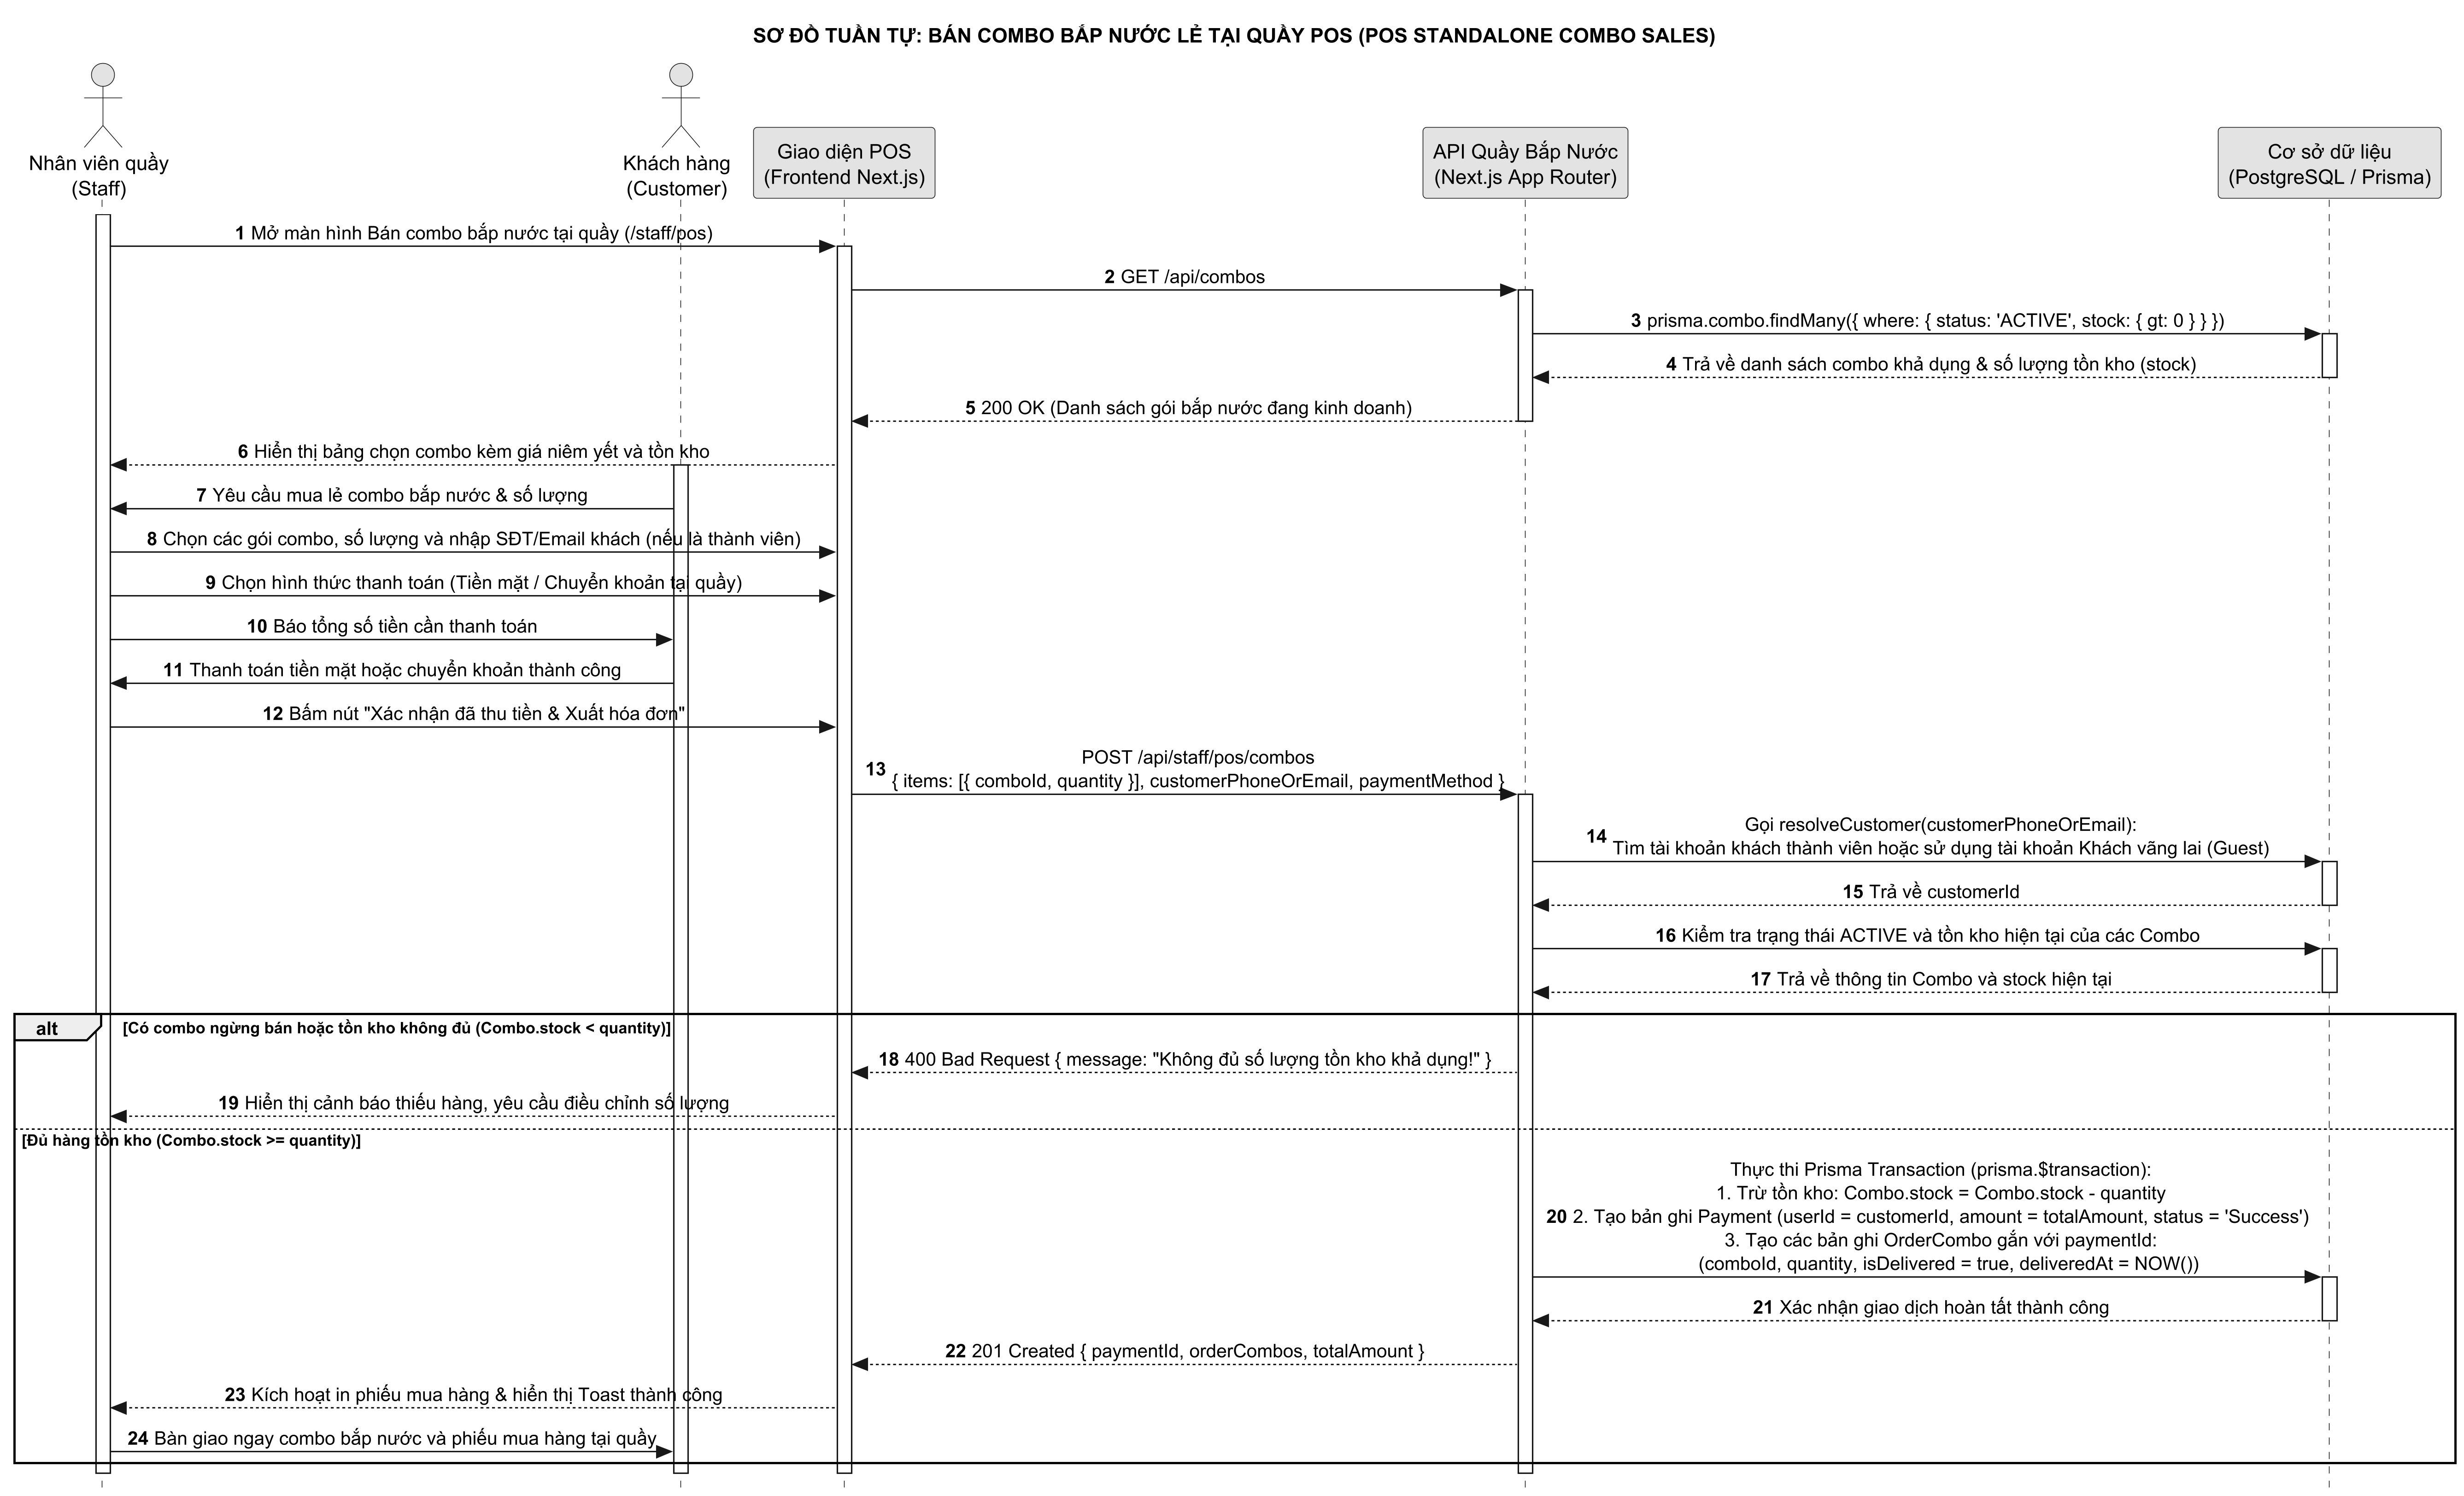
\includegraphics[width=\textwidth,height=0.80\textheight,keepaspectratio]{images/sequence/13_ban_combo_tai_quay_pos.png}
  \caption{Sequence Diagram: SƠ ĐỒ TUẦN TỰ: BÁN COMBO BẮP NƯỚC LẺ TẠI QUẦY POS (POS STANDALONE COMBO SALES)}
  \label{fig:seq_13}
\end{figure}

\subsection{SƠ ĐỒ TUẦN TỰ: SOÁT VÉ VÀO RẠP BẰNG MÃ QR (TICKET CHECK-IN)}
\begin{figure}[H]
  \centering
  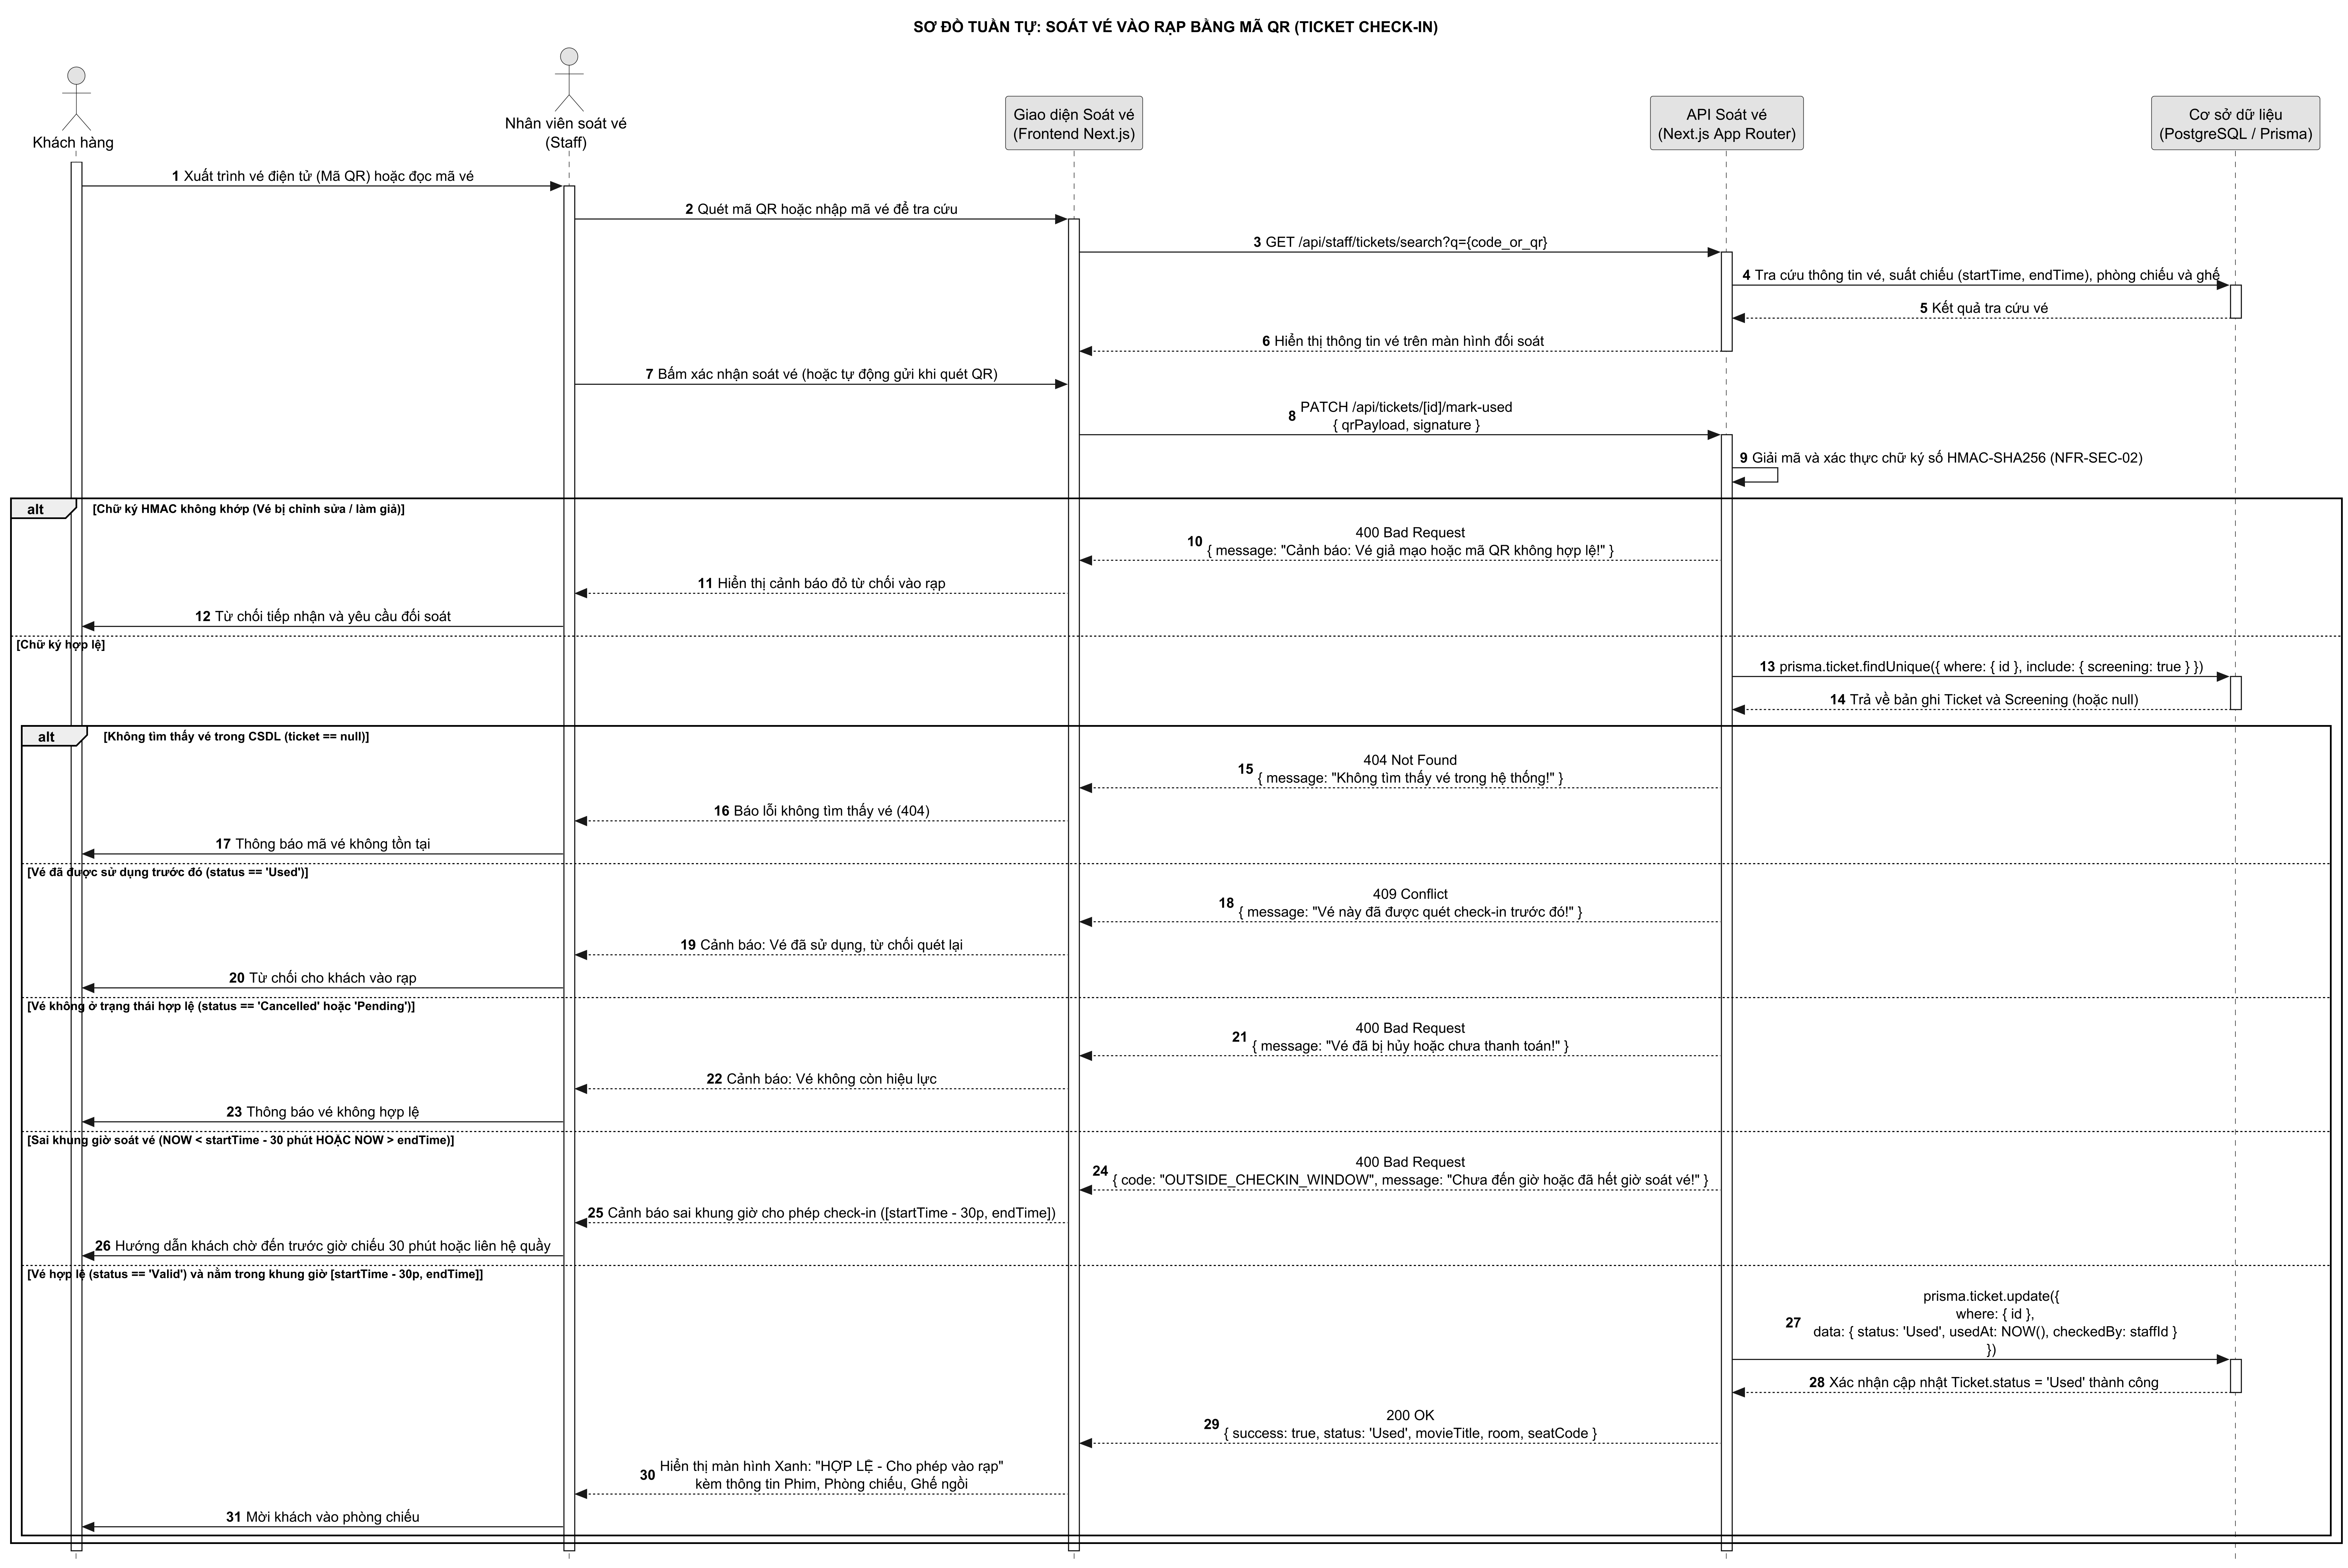
\includegraphics[width=\textwidth,height=0.80\textheight,keepaspectratio]{images/sequence/14_soat_ve_vao_rap.png}
  \caption{Sequence Diagram: SƠ ĐỒ TUẦN TỰ: SOÁT VÉ VÀO RẠP BẰNG MÃ QR (TICKET CHECK-IN)}
  \label{fig:seq_14}
\end{figure}

\subsection{SƠ ĐỒ TUẦN TỰ: GIAO NHẬN COMBO ĐÃ ĐẶT ONLINE (COMBO FULFILLMENT)}
\begin{figure}[H]
  \centering
  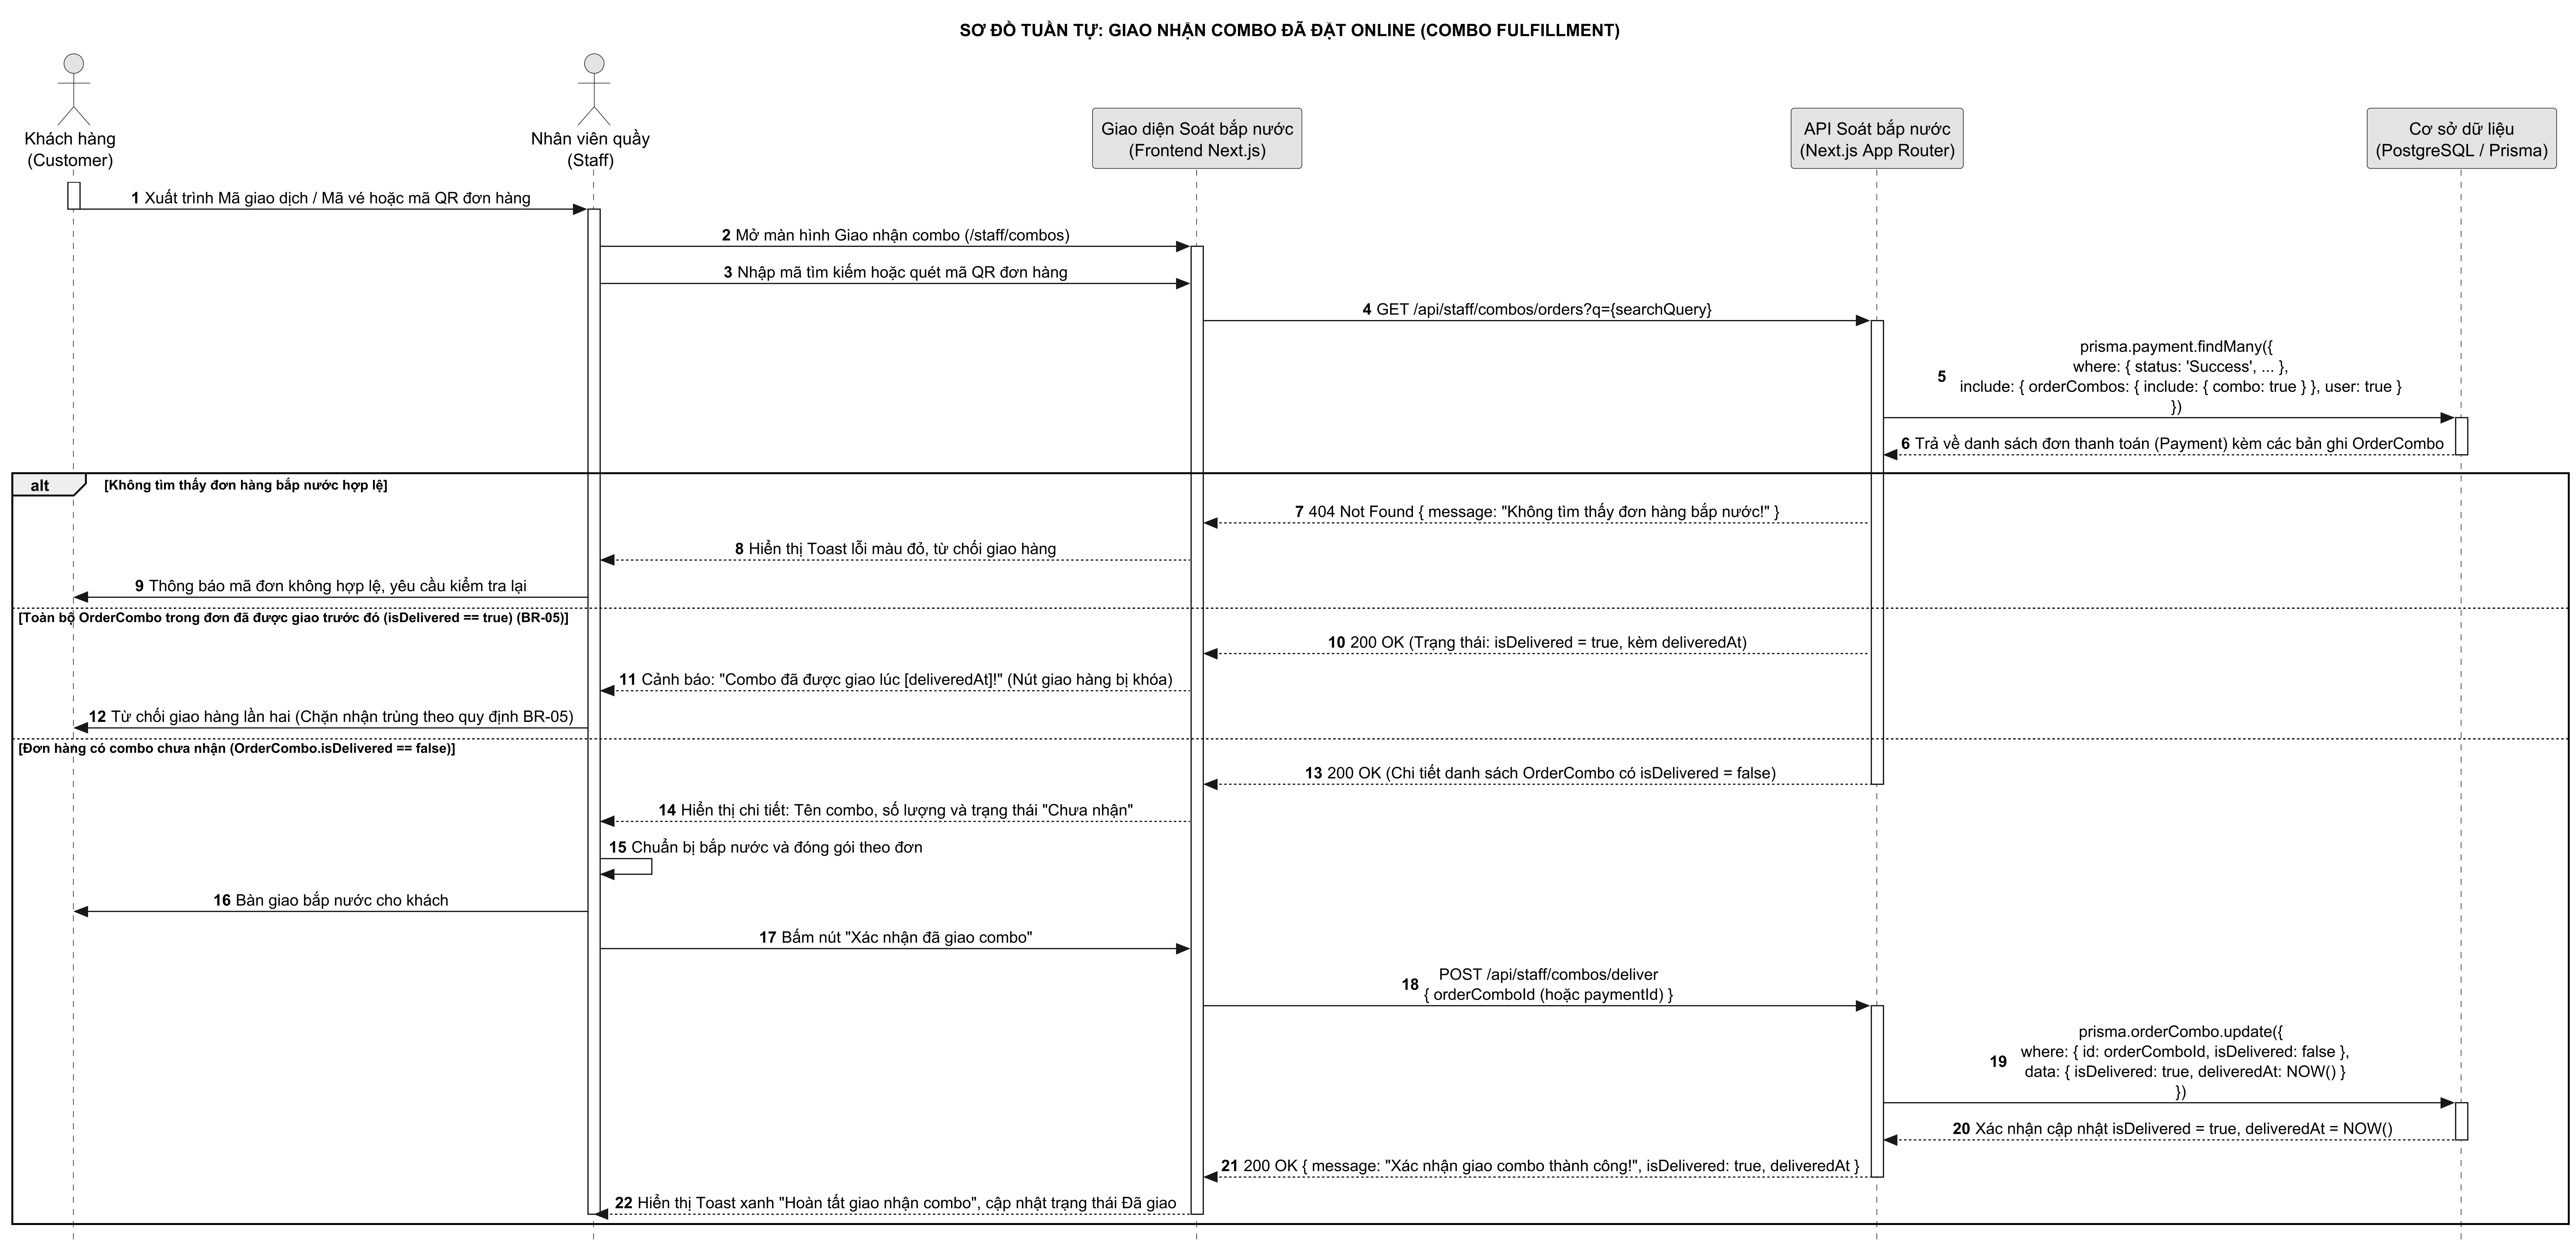
\includegraphics[width=\textwidth,height=0.80\textheight,keepaspectratio]{images/sequence/15_giao_nhan_combo_online.png}
  \caption{Sequence Diagram: SƠ ĐỒ TUẦN TỰ: GIAO NHẬN COMBO ĐÃ ĐẶT ONLINE (COMBO FULFILLMENT)}
  \label{fig:seq_15}
\end{figure}

\subsection{SƠ ĐỒ TUẦN TỰ: TRA CỨU \& QUẢN LÝ VÉ KHÁCH HÀNG (TICKET LOOKUP \& MANAGEMENT)}
\begin{figure}[H]
  \centering
  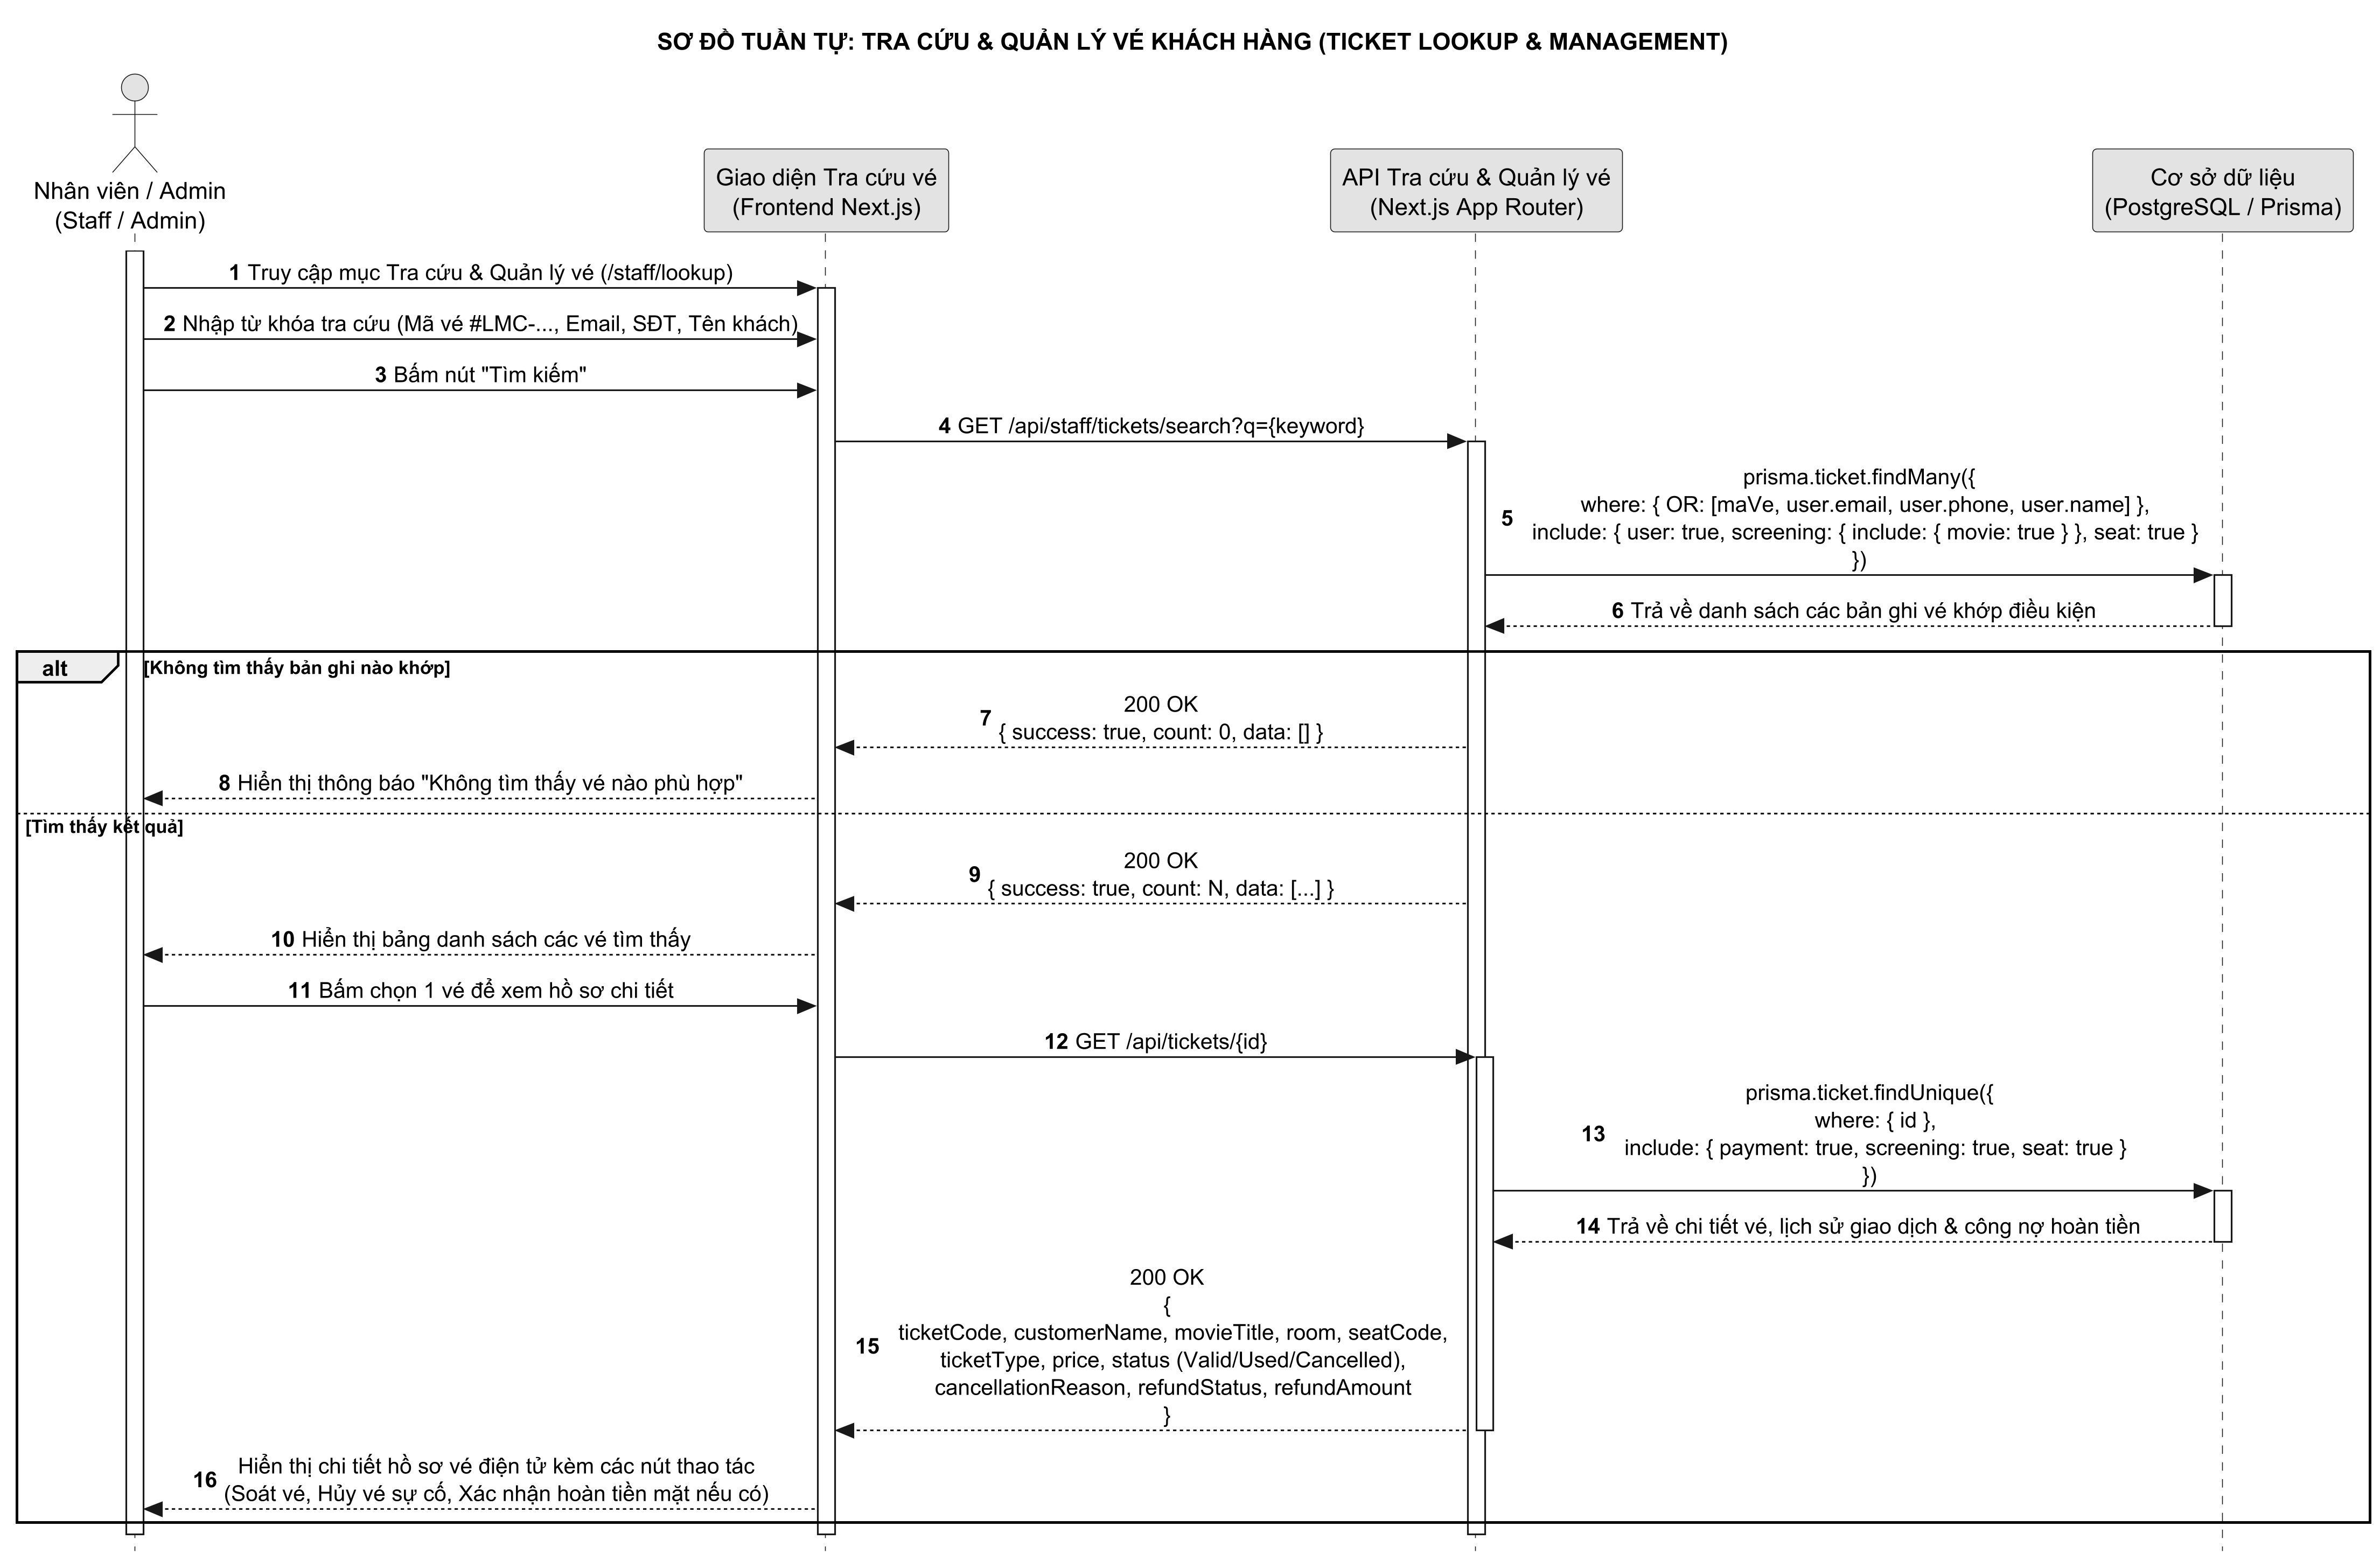
\includegraphics[width=\textwidth,height=0.80\textheight,keepaspectratio]{images/sequence/16_tra_cuu_quan_ly_ve.png}
  \caption{Sequence Diagram: SƠ ĐỒ TUẦN TỰ: TRA CỨU \& QUẢN LÝ VÉ KHÁCH HÀNG (TICKET LOOKUP \& MANAGEMENT)}
  \label{fig:seq_16}
\end{figure}

\subsection{SƠ ĐỒ TUẦN TỰ: KHÁCH HÀNG TỰ HỦY VÉ \& CẤP VOUCHER BỒI HOÀN (CUSTOMER CANCELLATION)}
\begin{figure}[H]
  \centering
  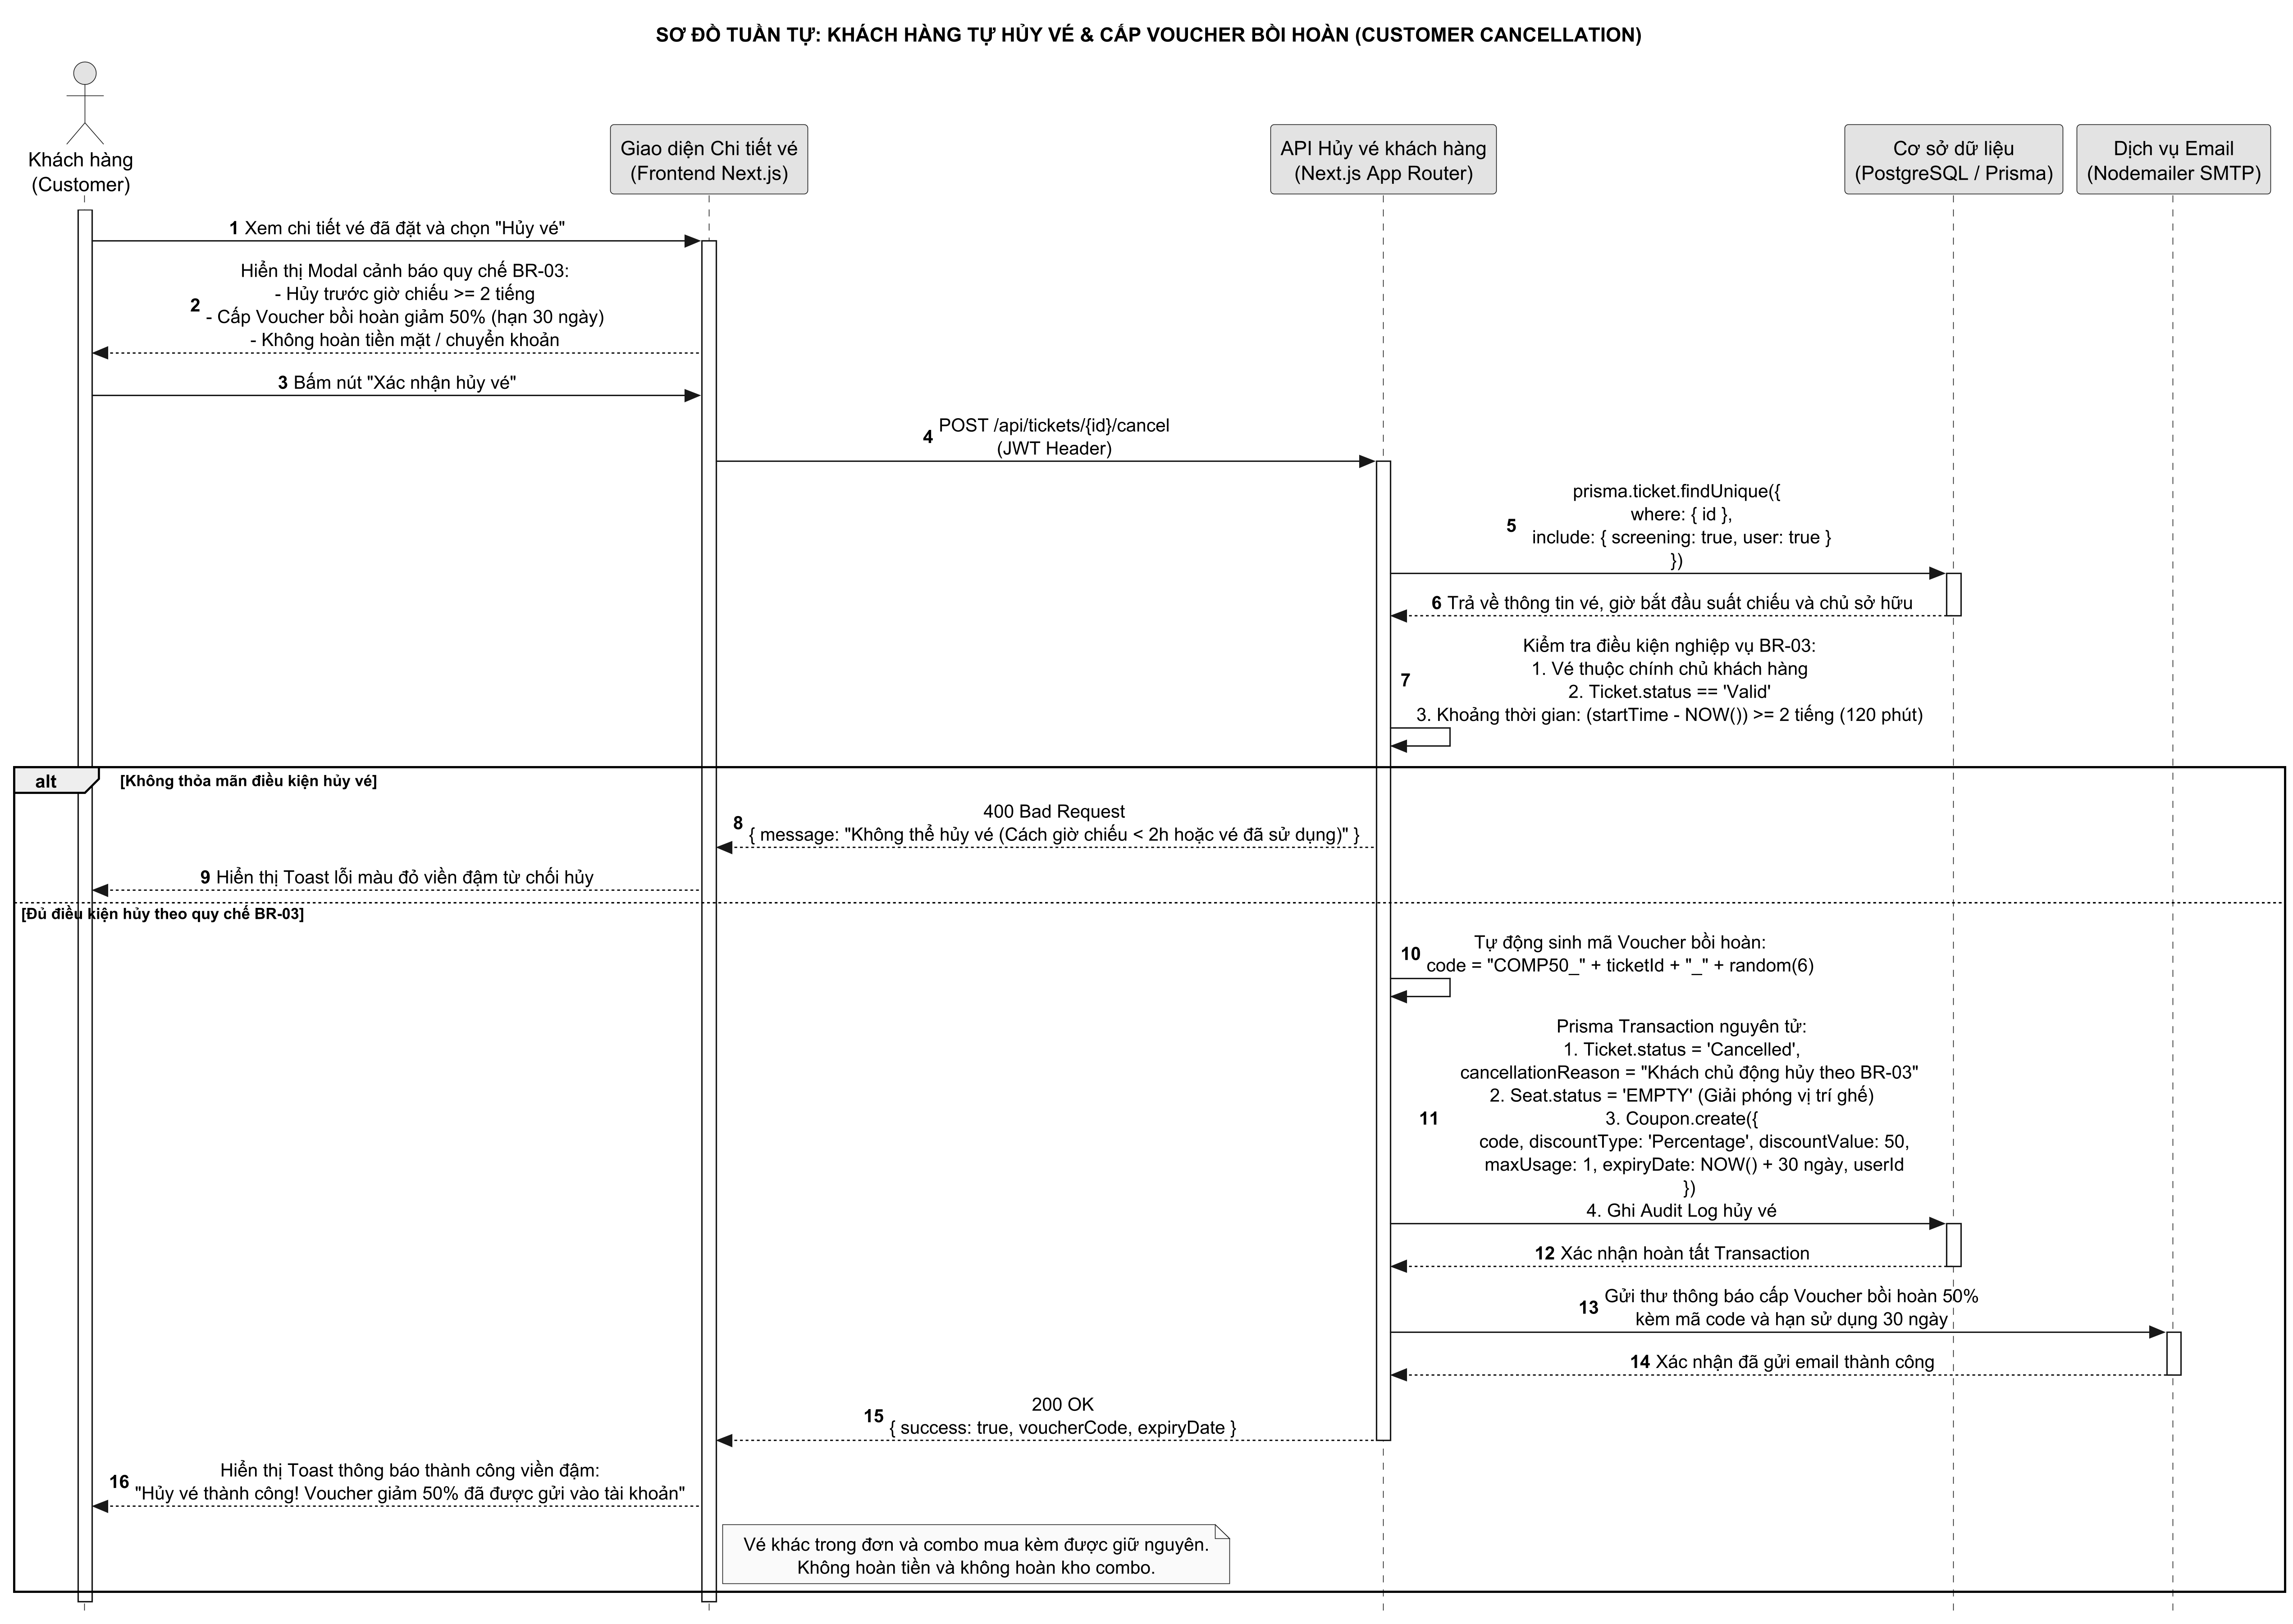
\includegraphics[width=\textwidth,height=0.80\textheight,keepaspectratio]{images/sequence/17_khach_huy_ve_nhan_voucher.png}
  \caption{Sequence Diagram: SƠ ĐỒ TUẦN TỰ: KHÁCH HÀNG TỰ HỦY VÉ \& CẤP VOUCHER BỒI HOÀN (CUSTOMER CANCELLATION)}
  \label{fig:seq_17}
\end{figure}

\subsection{SƠ ĐỒ TUẦN TỰ: HỦY VÉ SỰ CỐ RẠP \& BỒI HOÀN 1 BƯỚC (TIỀN MẶT / VOUCHER 100\%)}
\begin{figure}[H]
  \centering
  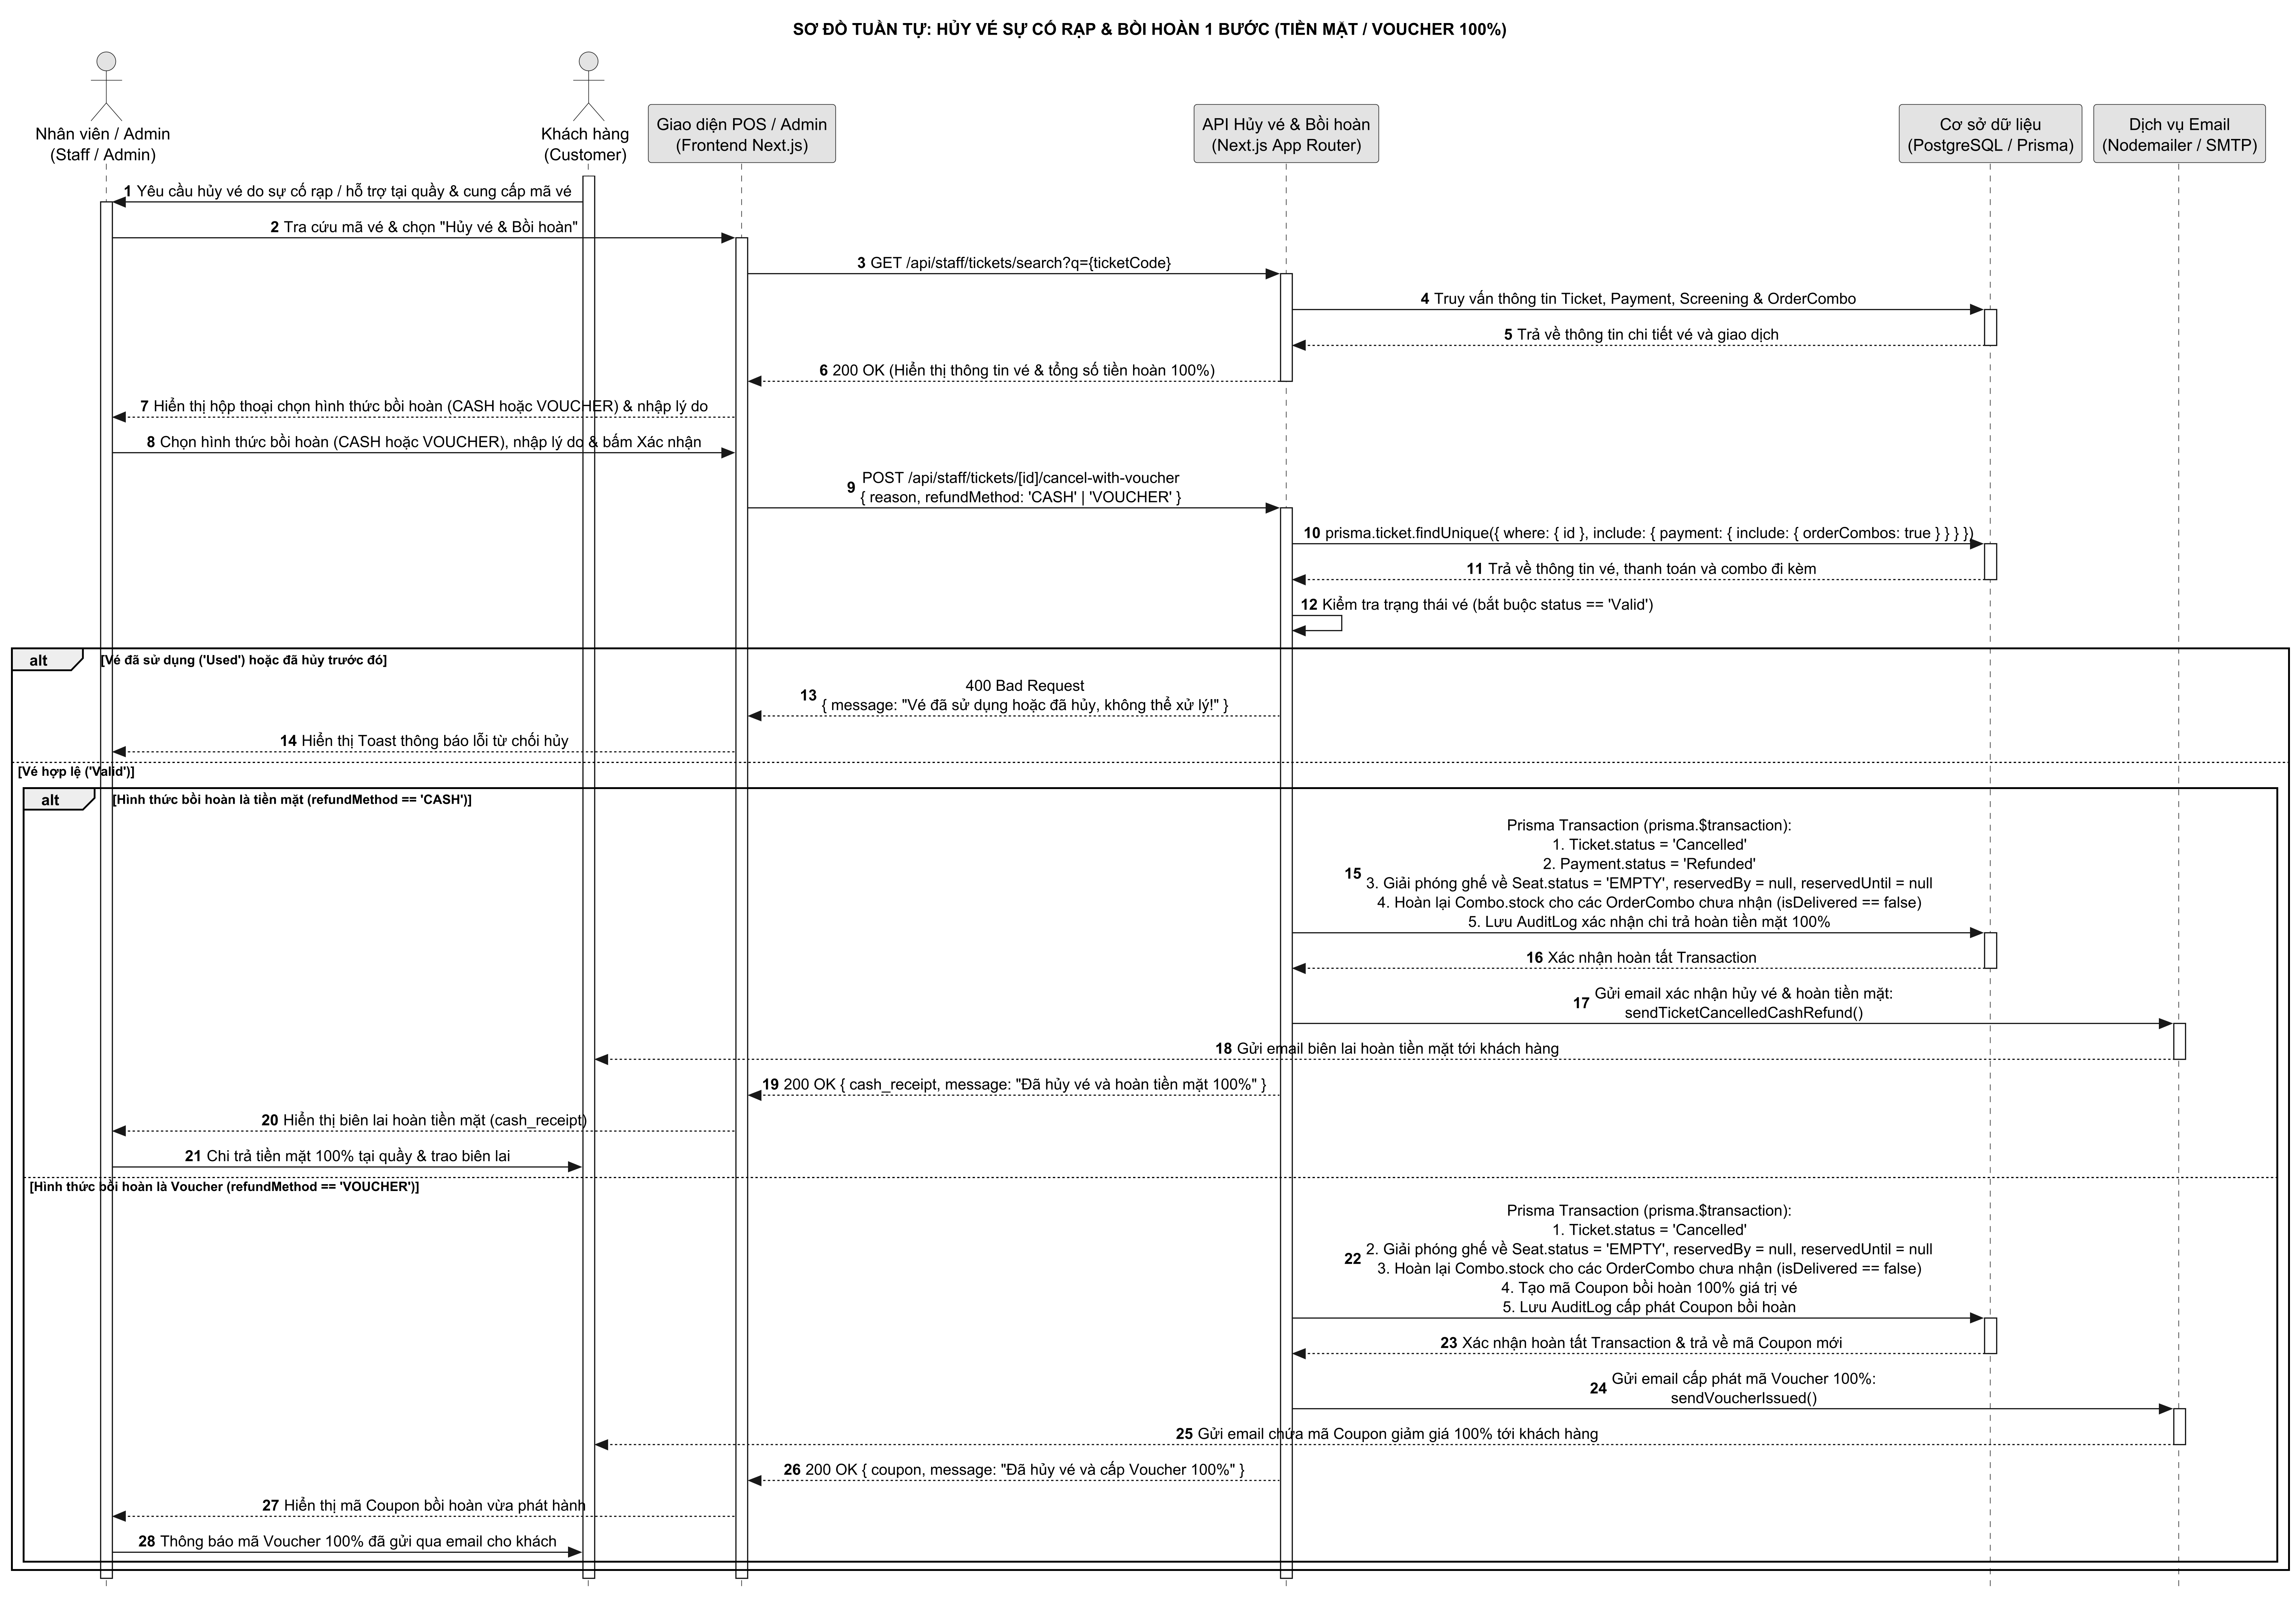
\includegraphics[width=\textwidth,height=0.80\textheight,keepaspectratio]{images/sequence/18_huy_ve_su_co_hoan_tien_mat.png}
  \caption{Sequence Diagram: SƠ ĐỒ TUẦN TỰ: HỦY VÉ SỰ CỐ RẠP \& BỒI HOÀN 1 BƯỚC (TIỀN MẶT / VOUCHER 100\%)}
  \label{fig:seq_18}
\end{figure}

\subsection{SƠ ĐỒ TUẦN TỰ: KHÁCH HÀNG ĐÁNH GIÁ \& BÌNH LUẬN PHIM (MOVIE REVIEW)}
\begin{figure}[H]
  \centering
  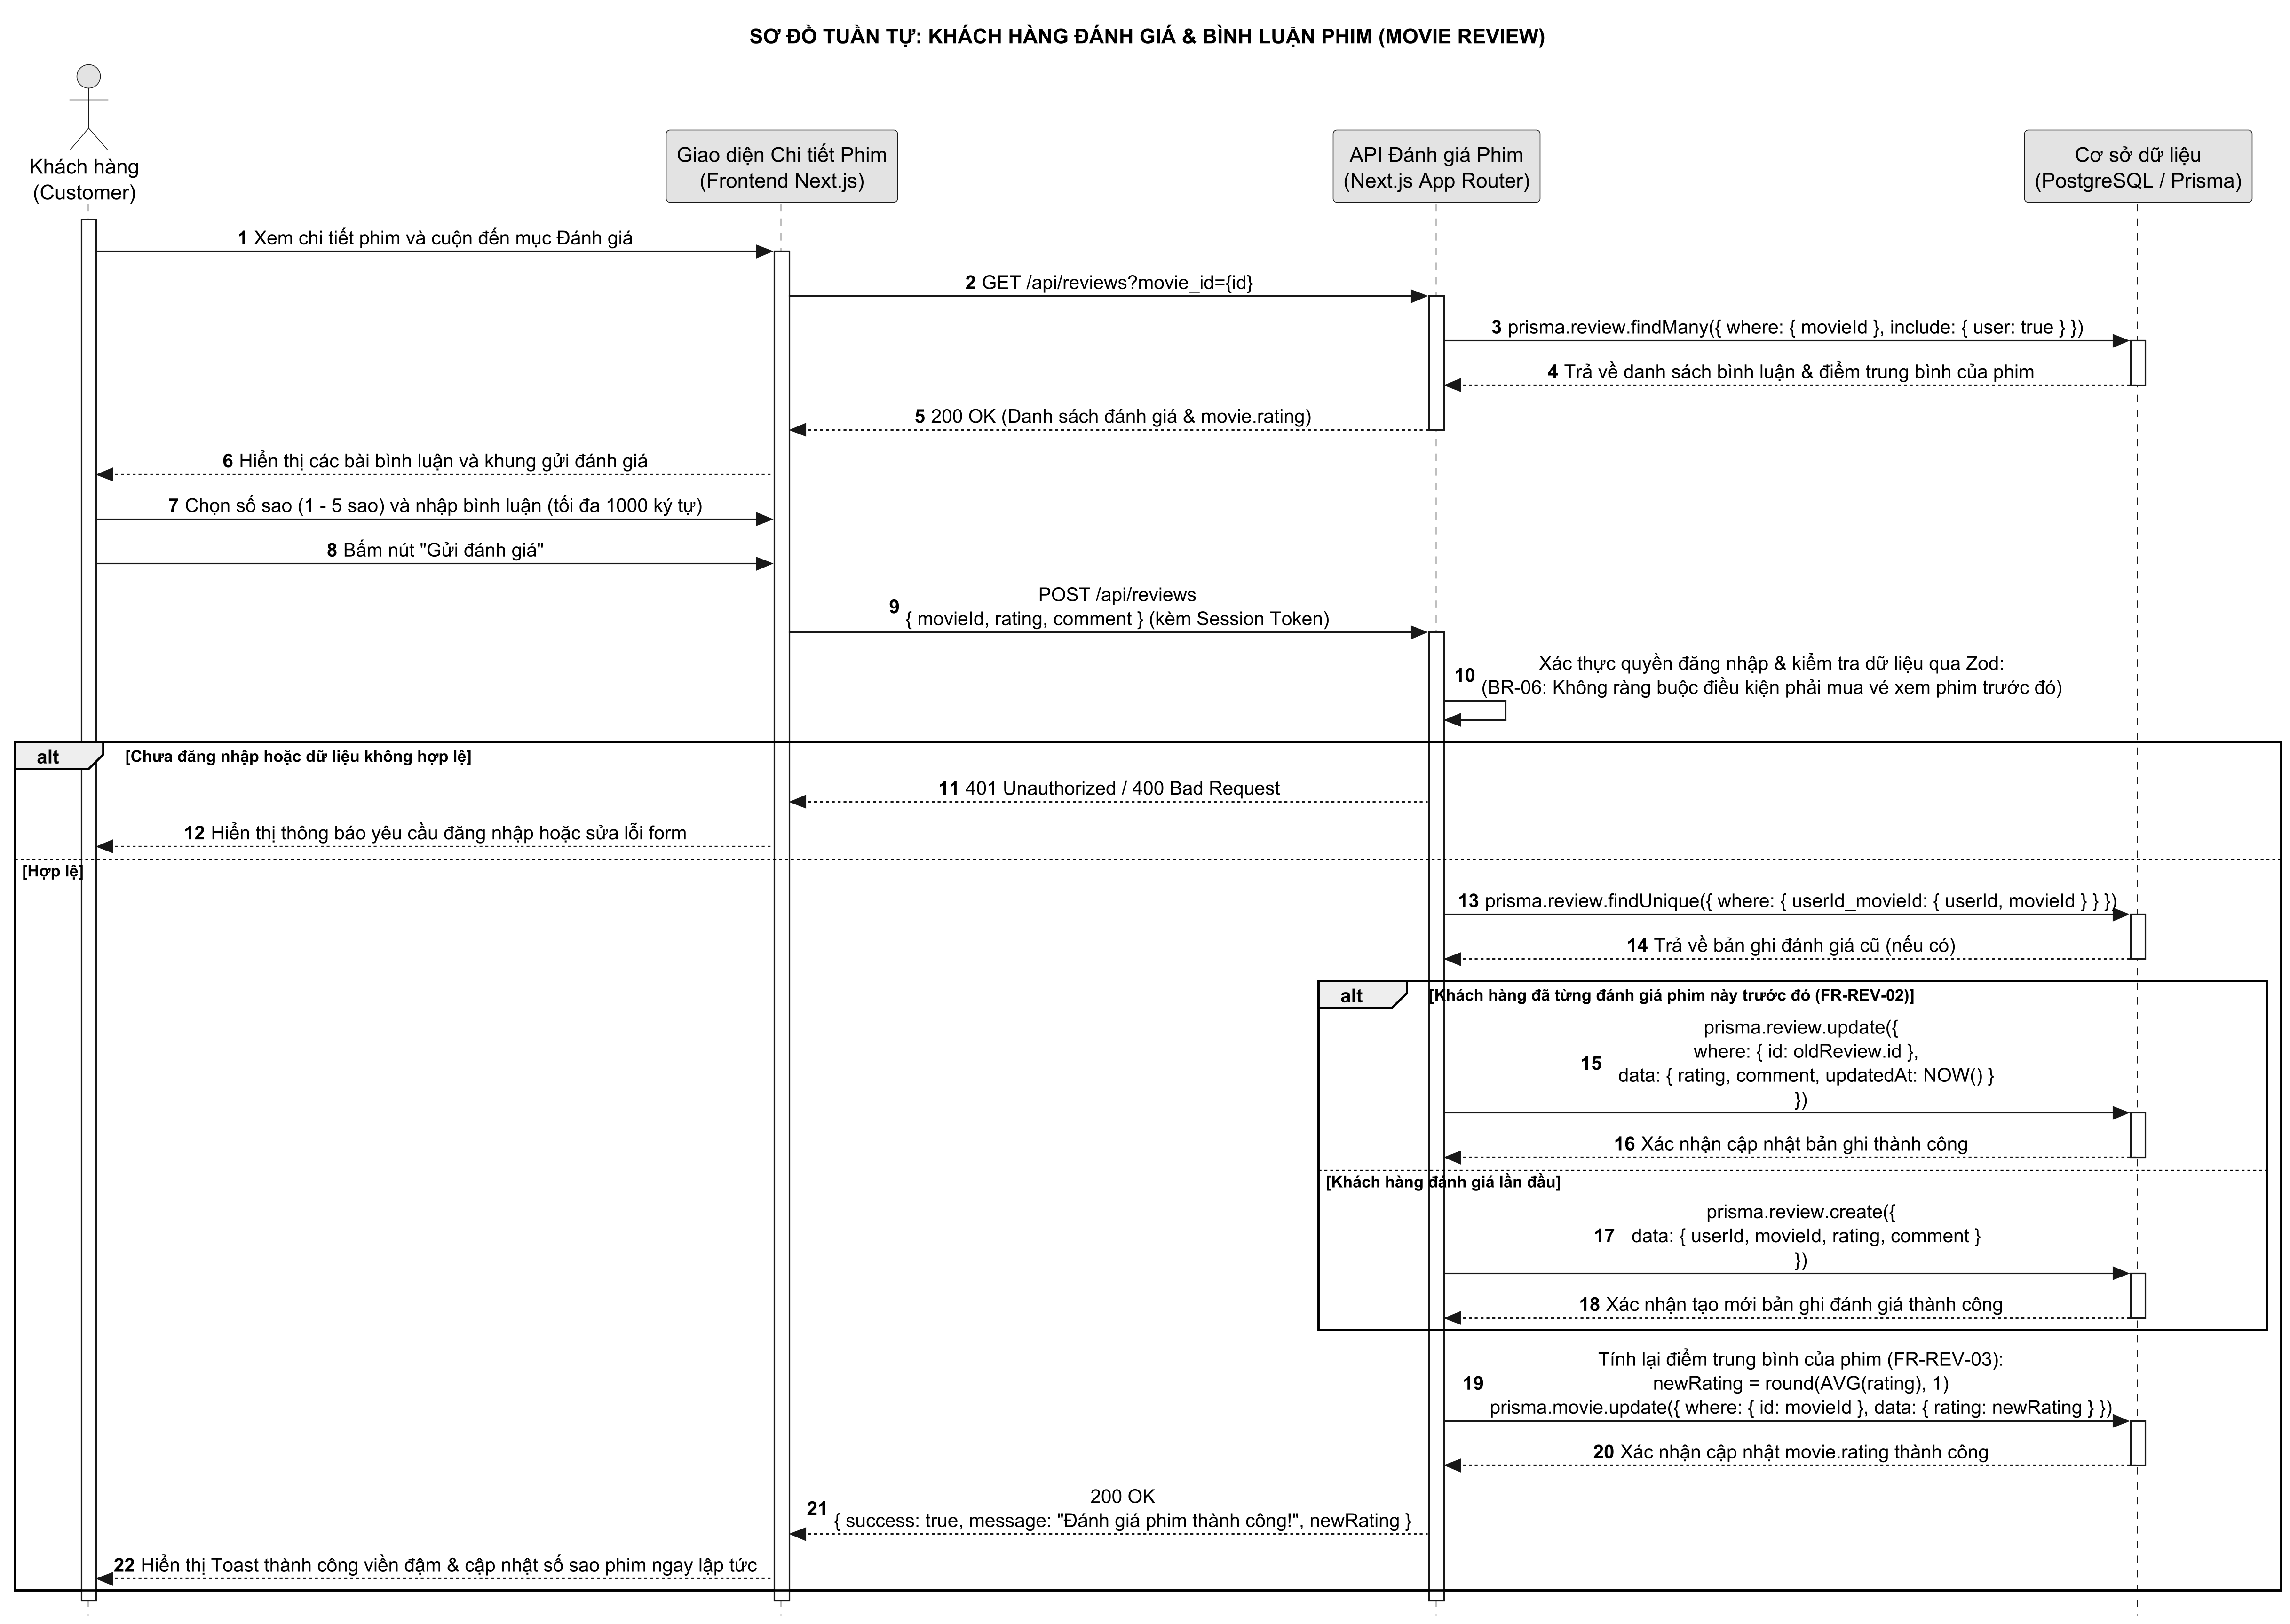
\includegraphics[width=\textwidth,height=0.80\textheight,keepaspectratio]{images/sequence/19_khach_danh_gia_phim.png}
  \caption{Sequence Diagram: SƠ ĐỒ TUẦN TỰ: KHÁCH HÀNG ĐÁNH GIÁ \& BÌNH LUẬN PHIM (MOVIE REVIEW)}
  \label{fig:seq_19}
\end{figure}

\subsection{SƠ ĐỒ TUẦN TỰ: QUẢN LÝ \& KIỂM DUYỆT ĐÁNH GIÁ PHIM (ADMIN REVIEW MODERATION)}
\begin{figure}[H]
  \centering
  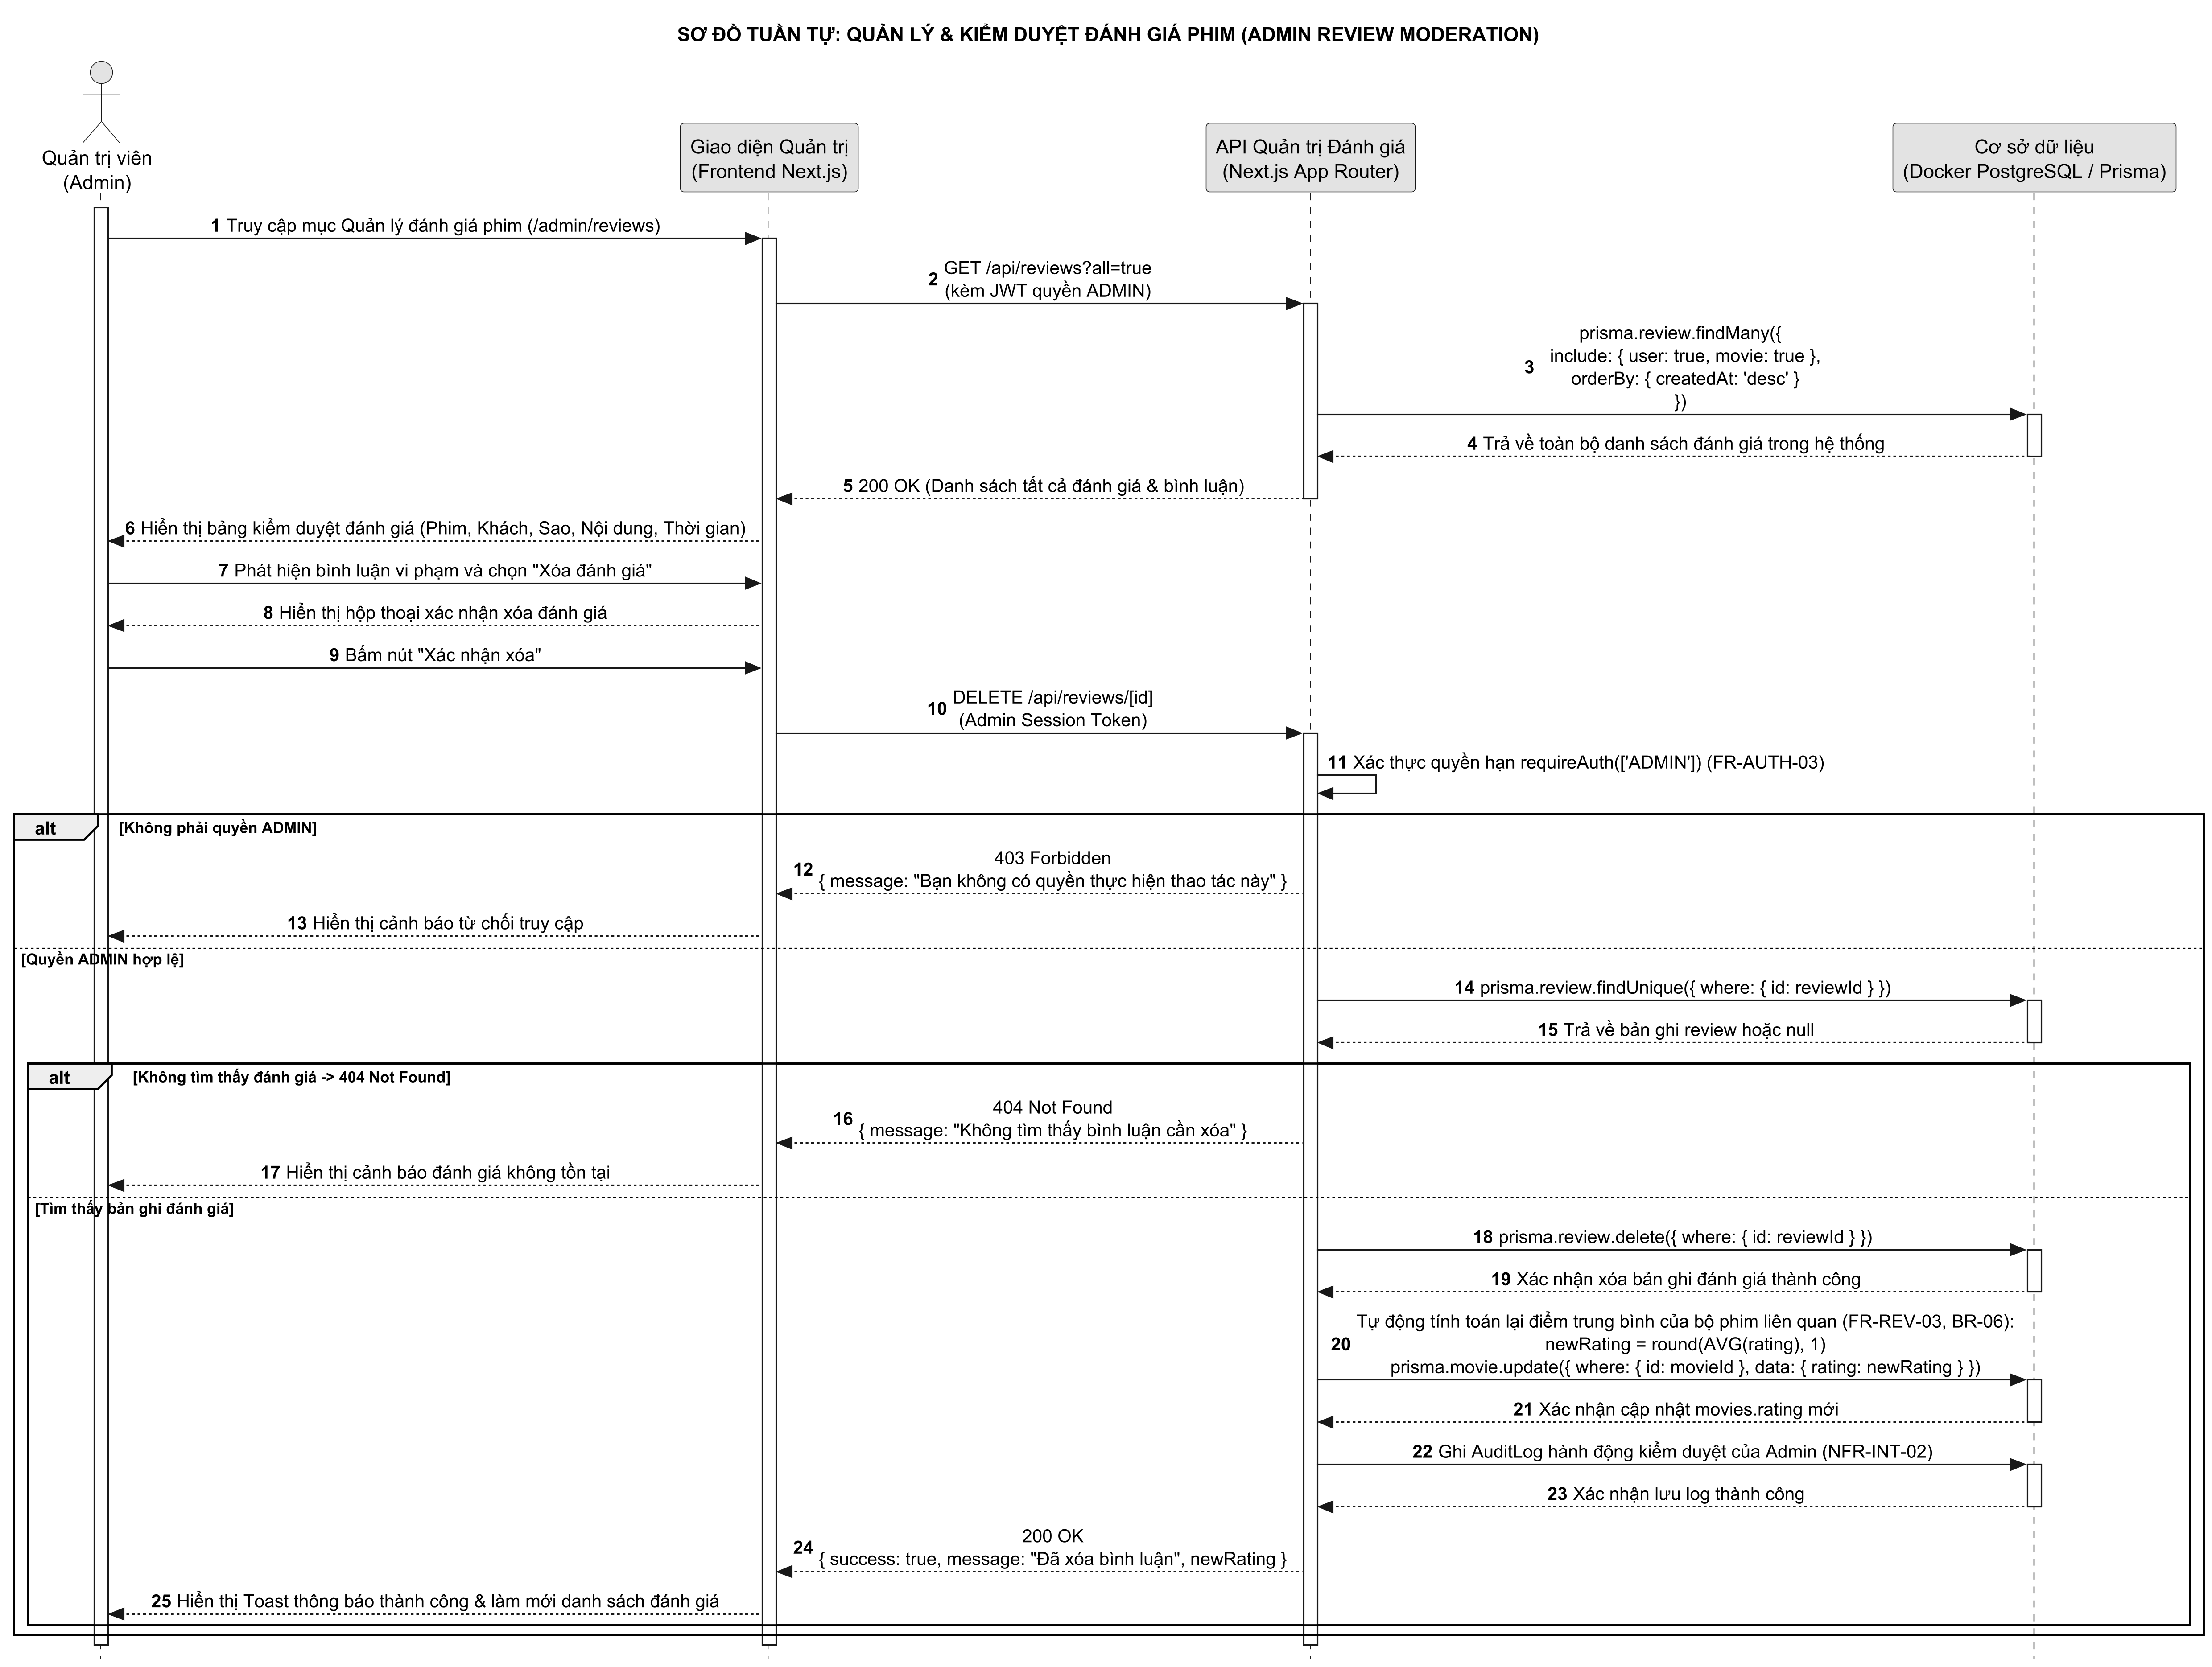
\includegraphics[width=\textwidth,height=0.80\textheight,keepaspectratio]{images/sequence/20_admin_quan_ly_danh_gia.png}
  \caption{Sequence Diagram: SƠ ĐỒ TUẦN TỰ: QUẢN LÝ \& KIỂM DUYỆT ĐÁNH GIÁ PHIM (ADMIN REVIEW MODERATION)}
  \label{fig:seq_20}
\end{figure}

\subsection{SƠ ĐỒ TUẦN TỰ: QUẢN TRỊ DANH MỤC PHIM (TỔNG QUAN)}
\begin{figure}[H]
  \centering
  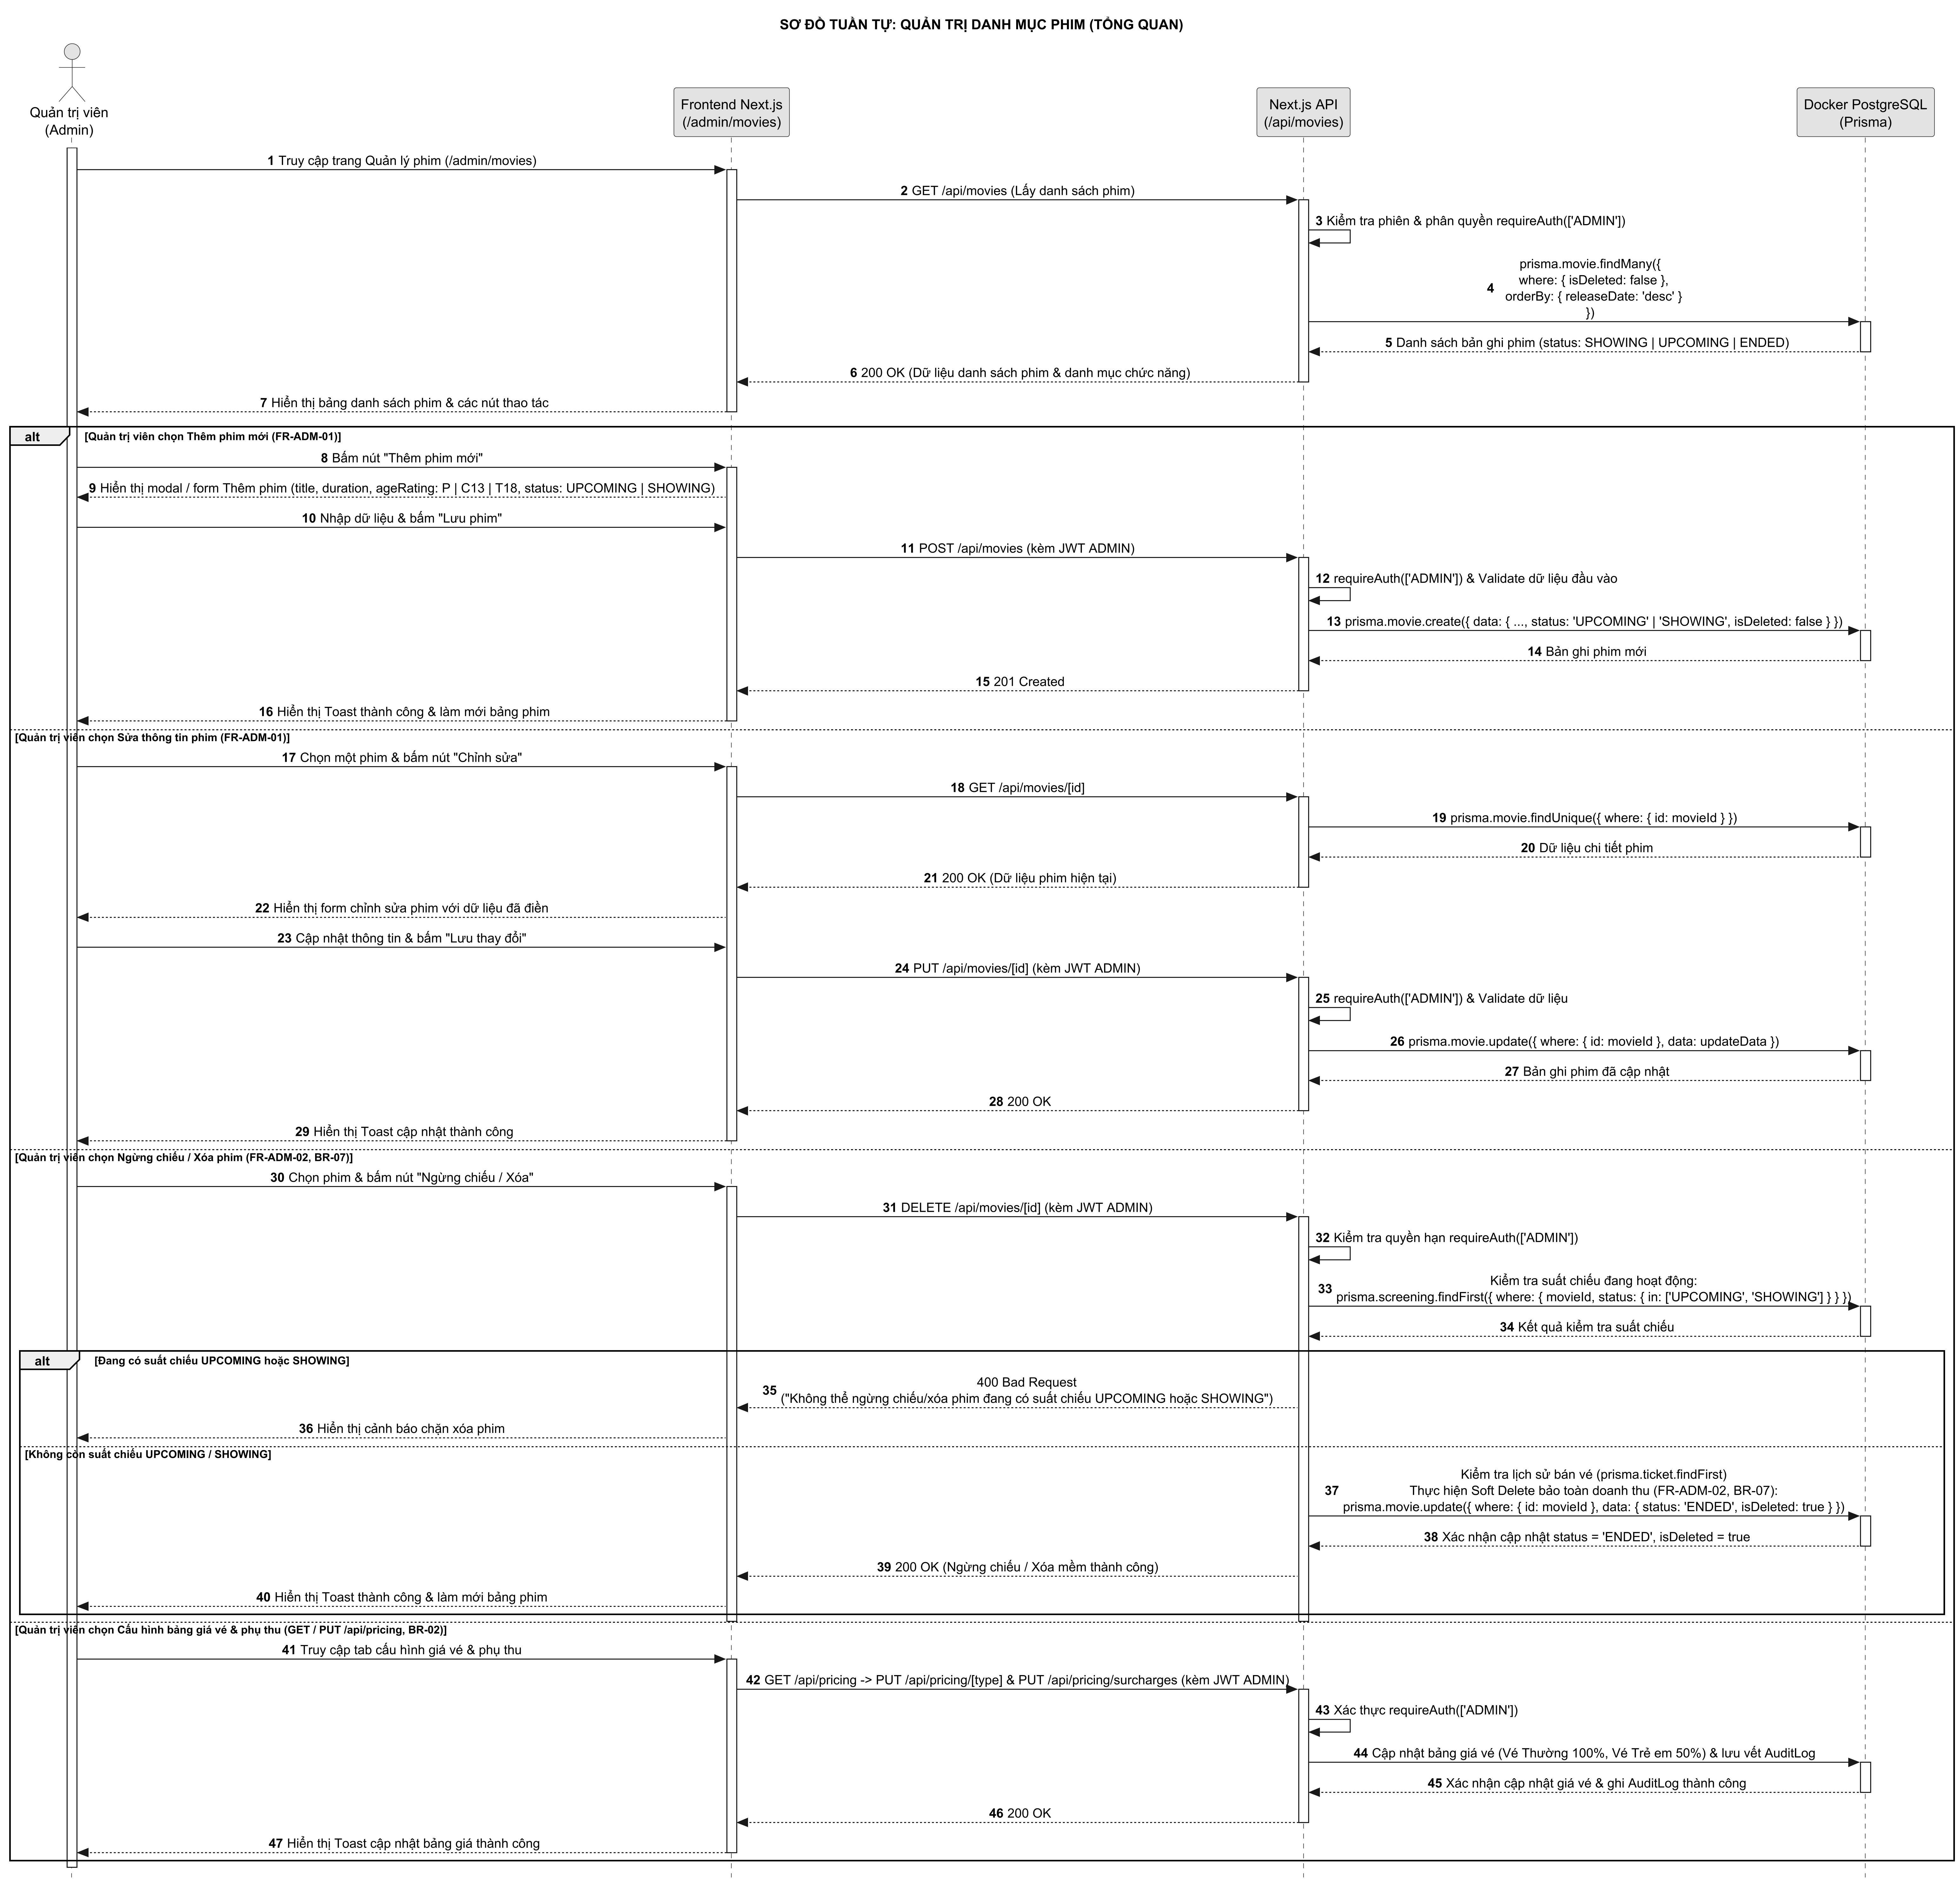
\includegraphics[width=\textwidth,height=0.80\textheight,keepaspectratio]{images/sequence/21_quan_ly_phim_tong_quan.png}
  \caption{Sequence Diagram: SƠ ĐỒ TUẦN TỰ: QUẢN TRỊ DANH MỤC PHIM (TỔNG QUAN)}
  \label{fig:seq_21}
\end{figure}

\subsection{SƠ ĐỒ TUẦN TỰ: THÊM PHIM MỚI (FR-ADM-01, BR-02)}
\begin{figure}[H]
  \centering
  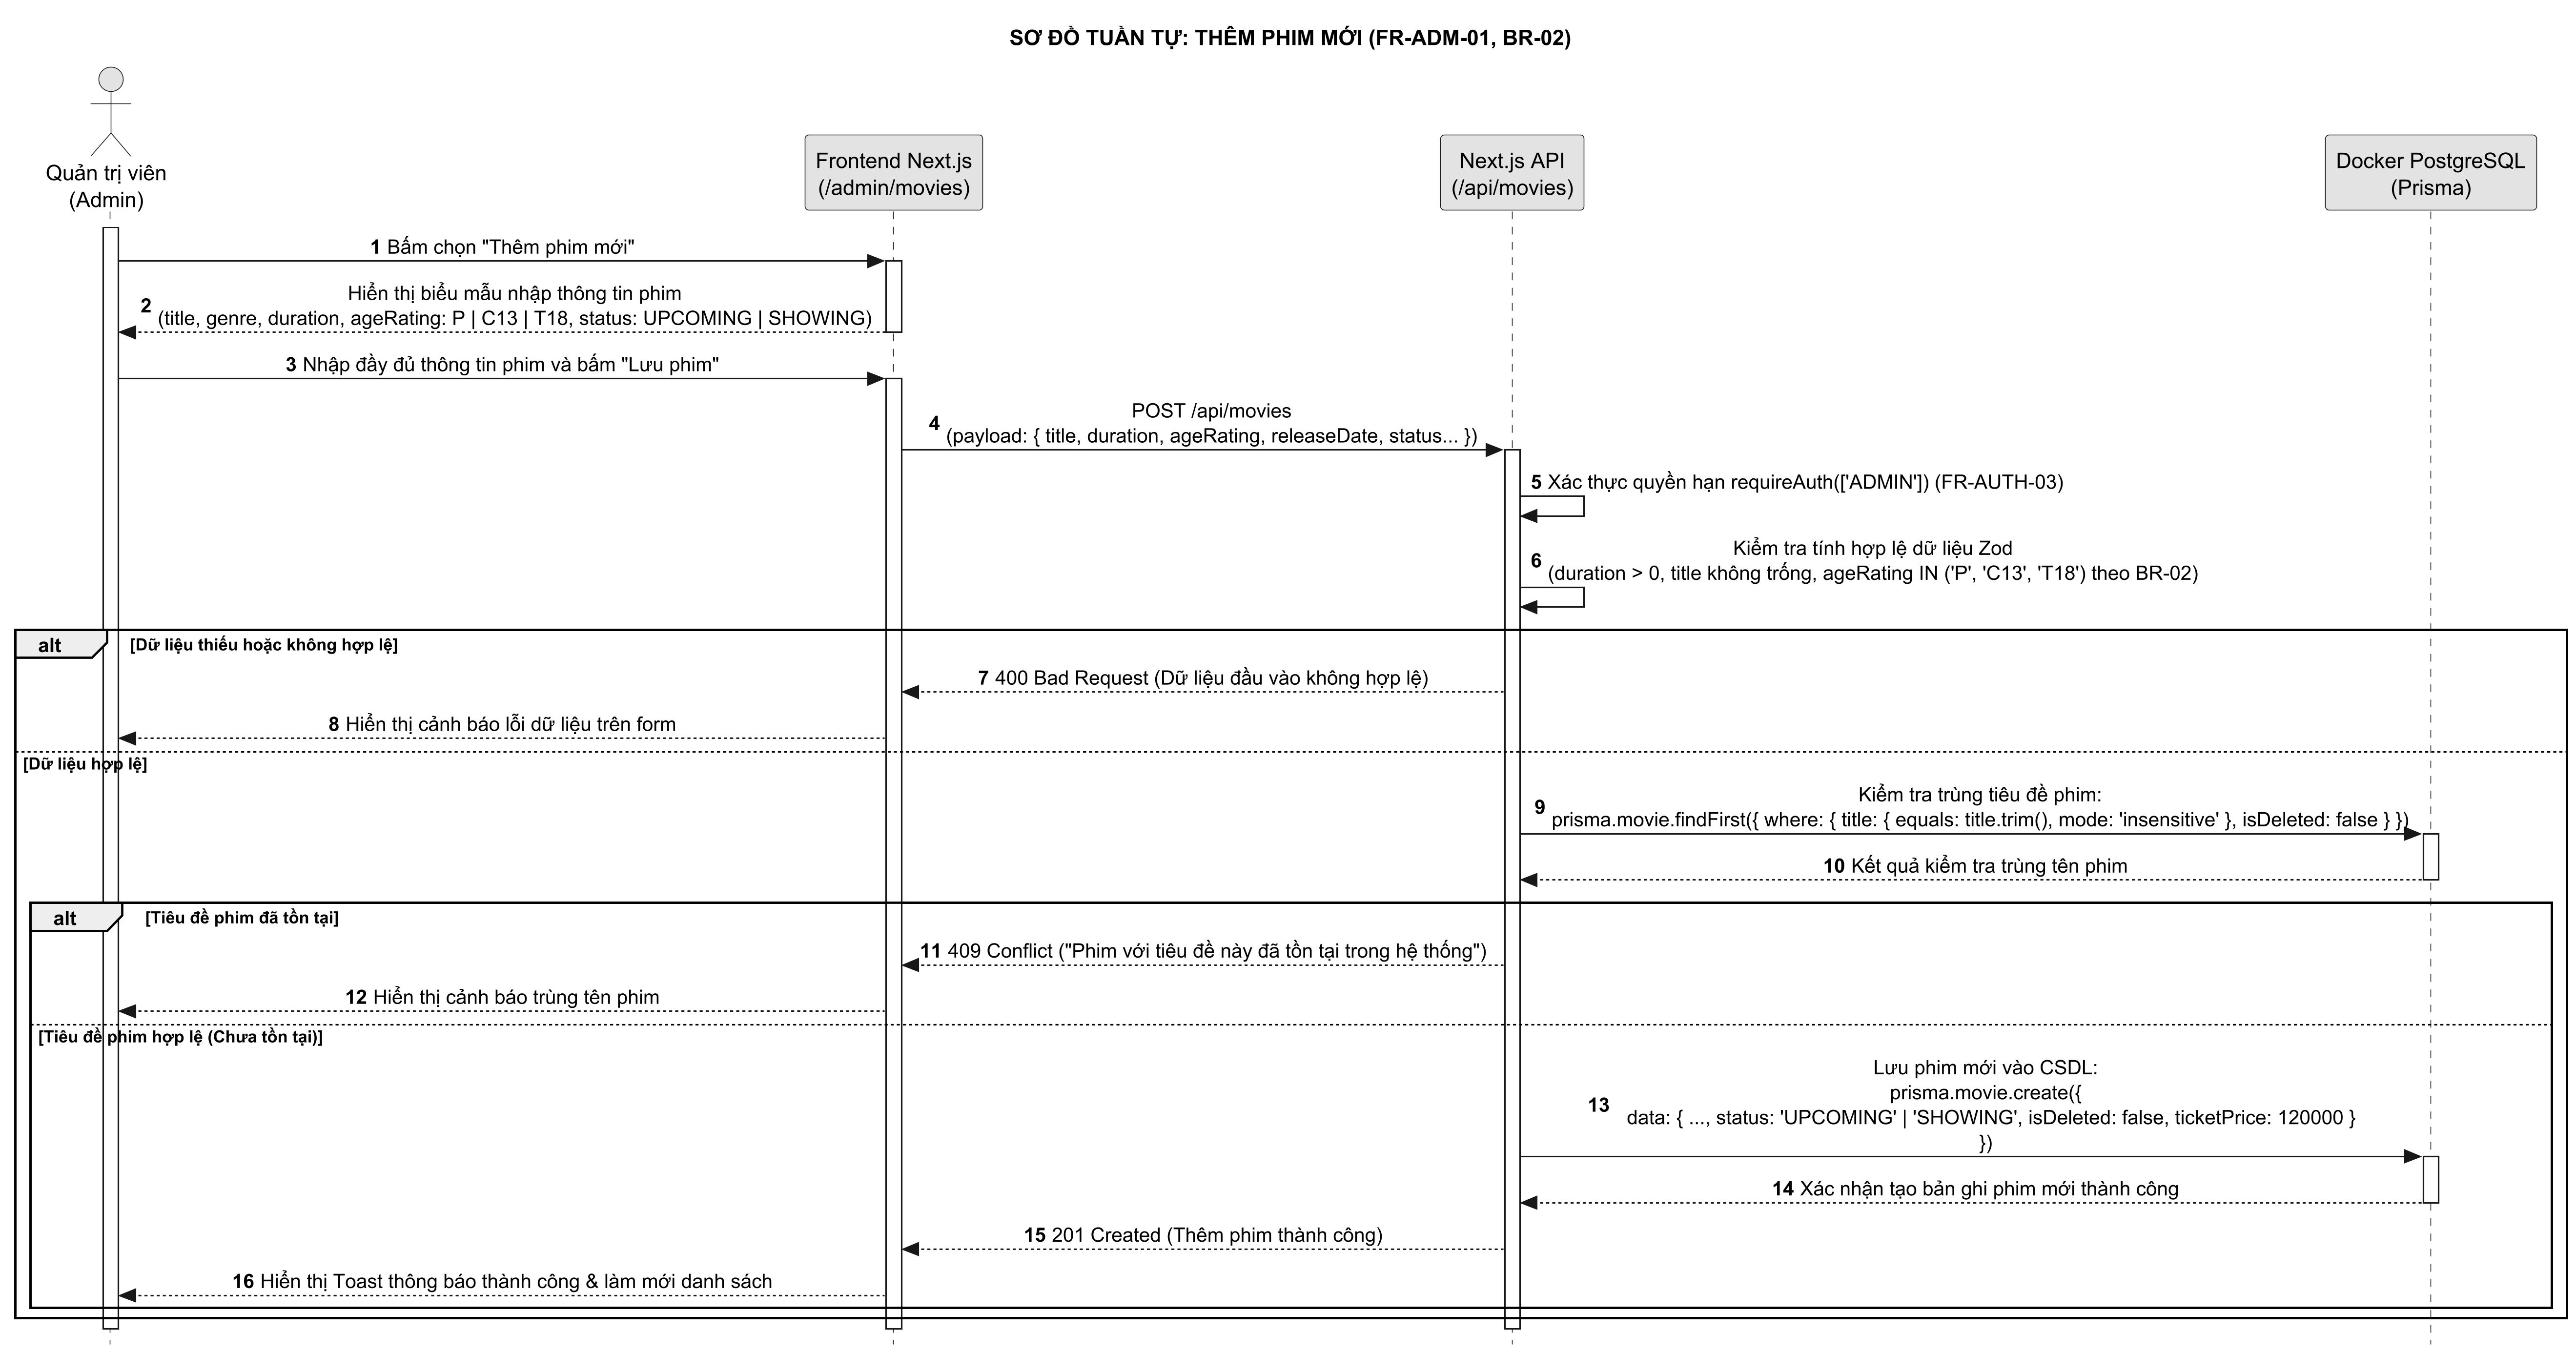
\includegraphics[width=\textwidth,height=0.80\textheight,keepaspectratio]{images/sequence/22_them_phim.png}
  \caption{Sequence Diagram: SƠ ĐỒ TUẦN TỰ: THÊM PHIM MỚI (FR-ADM-01, BR-02)}
  \label{fig:seq_22}
\end{figure}

\subsection{SƠ ĐỒ TUẦN TỰ: CHỈNH SỬA THÔNG TIN PHIM (FR-ADM-01, BR-02)}
\begin{figure}[H]
  \centering
  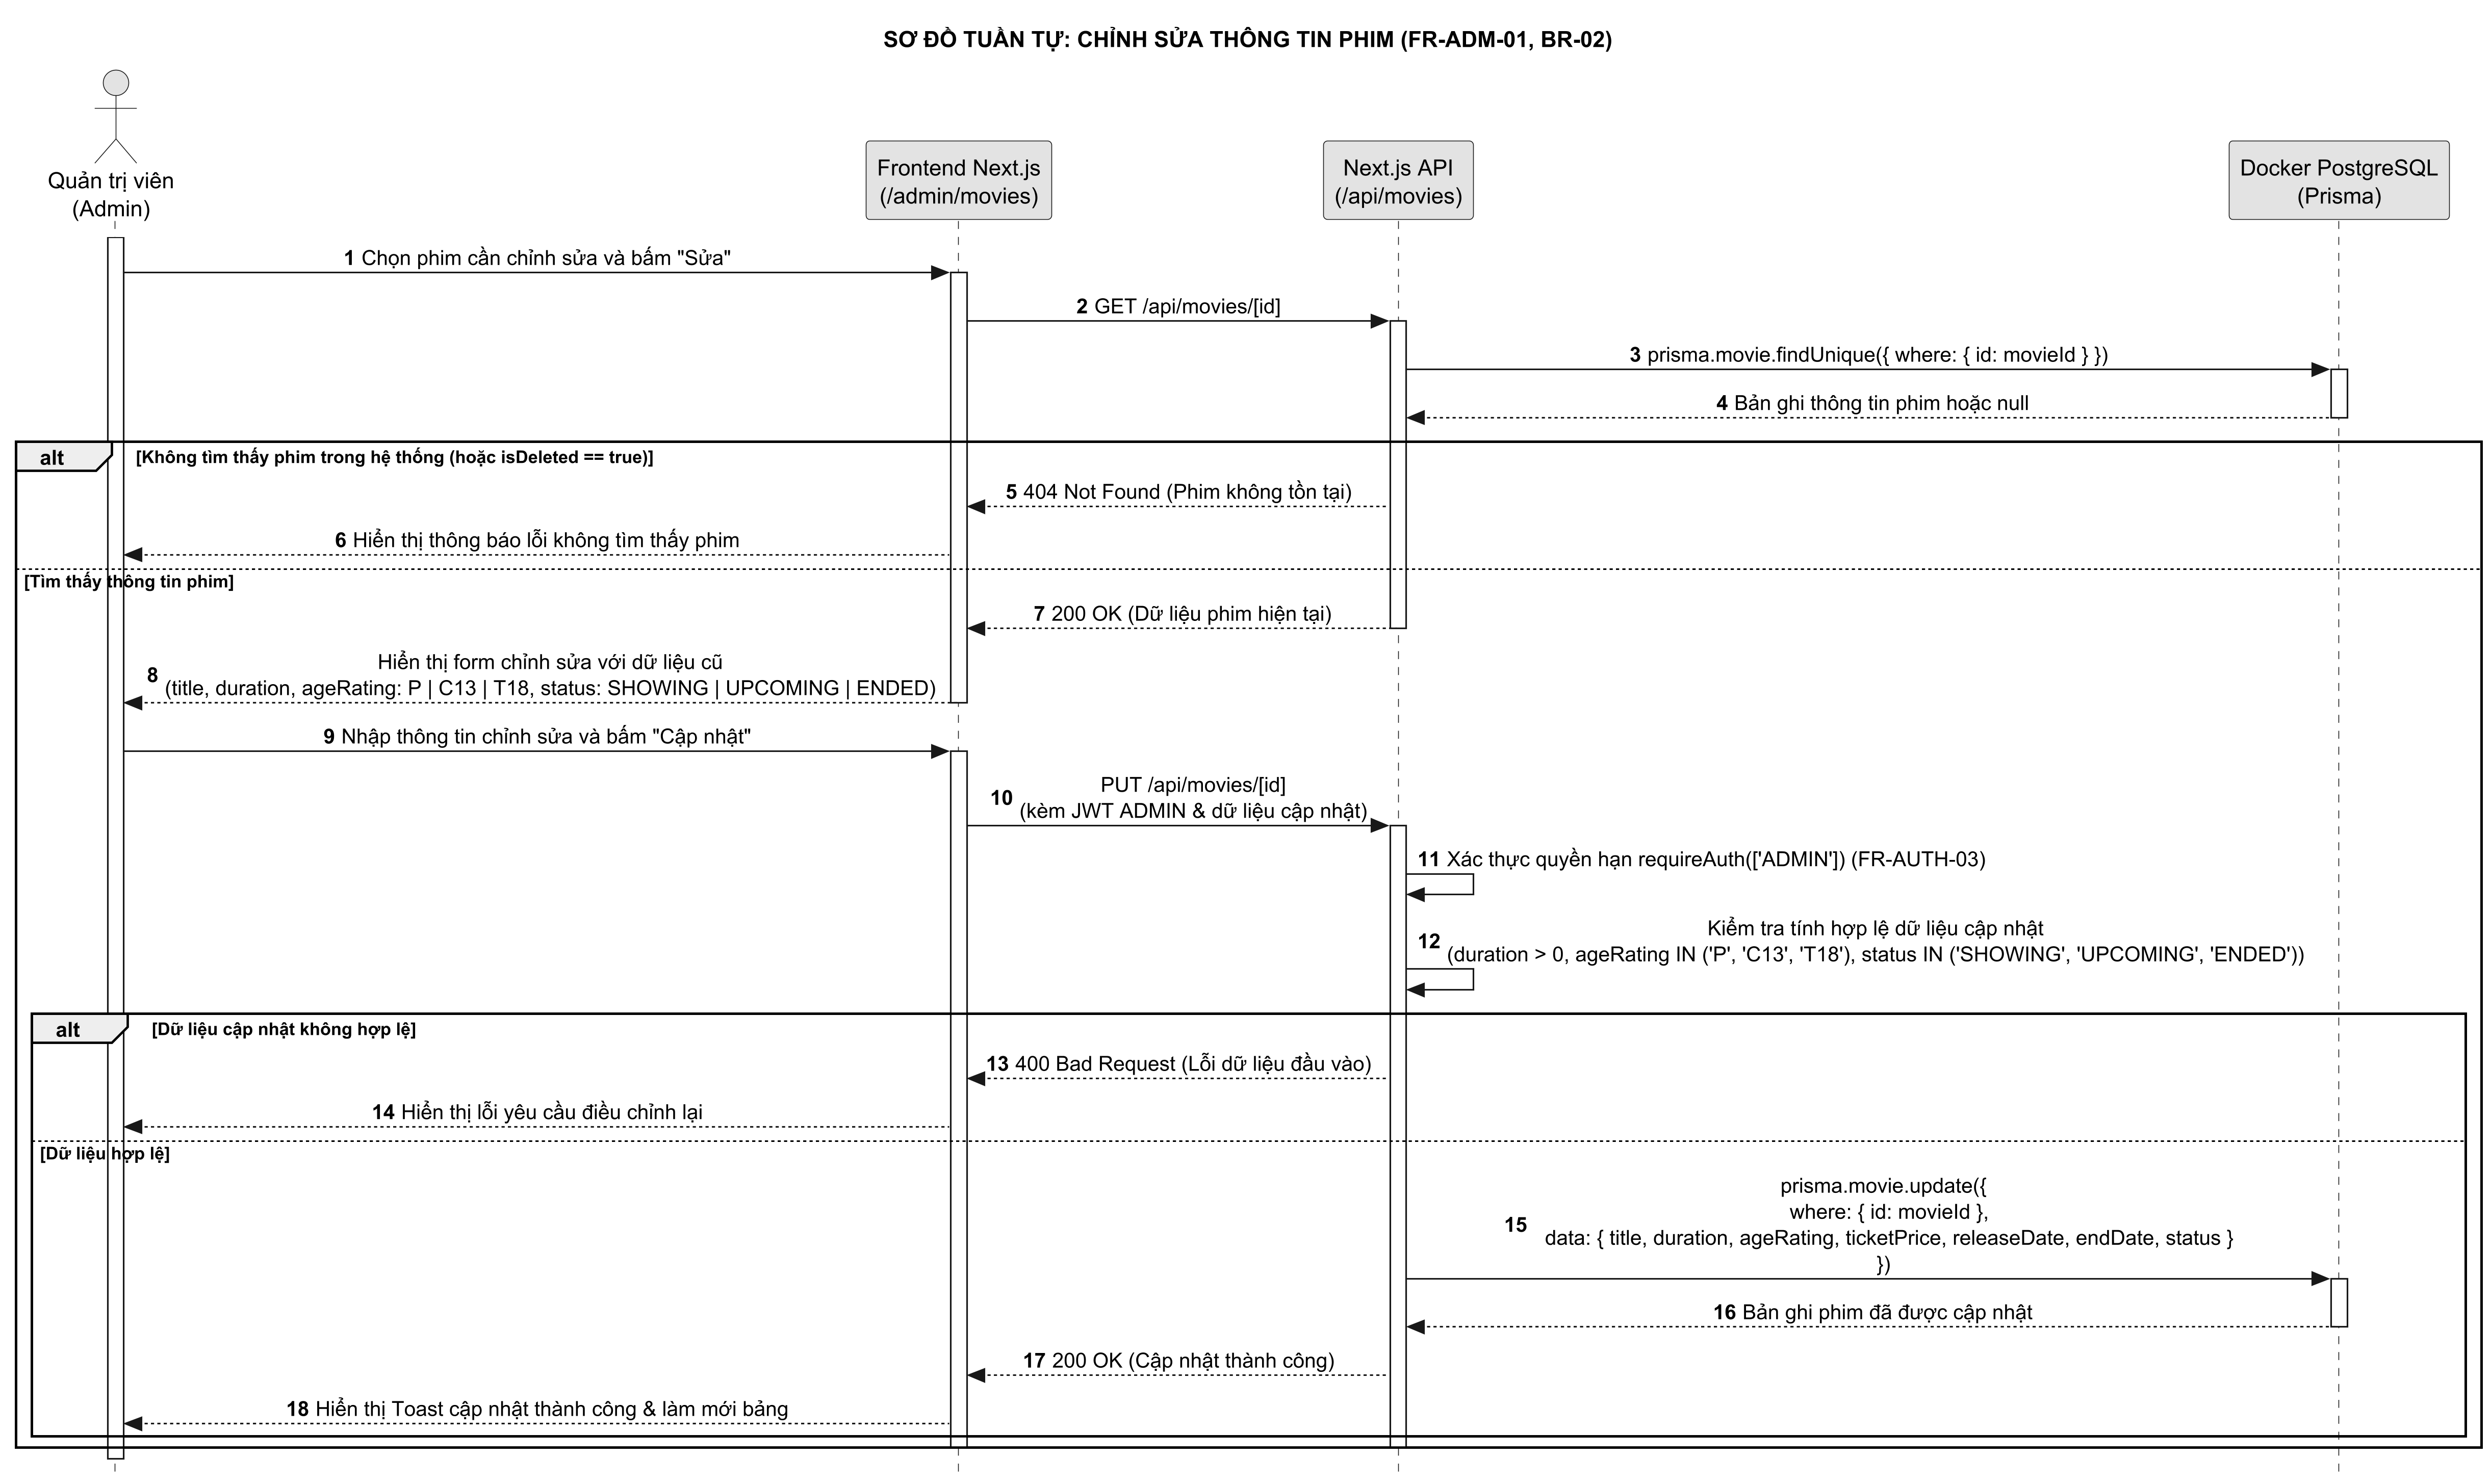
\includegraphics[width=\textwidth,height=0.80\textheight,keepaspectratio]{images/sequence/23_sua_phim.png}
  \caption{Sequence Diagram: SƠ ĐỒ TUẦN TỰ: CHỈNH SỬA THÔNG TIN PHIM (FR-ADM-01, BR-02)}
  \label{fig:seq_23}
\end{figure}

\subsection{SƠ ĐỒ TUẦN TỰ: NGỪNG CHIẾU / XÓA MỀM PHIM (FR-ADM-02, BR-07)}
\begin{figure}[H]
  \centering
  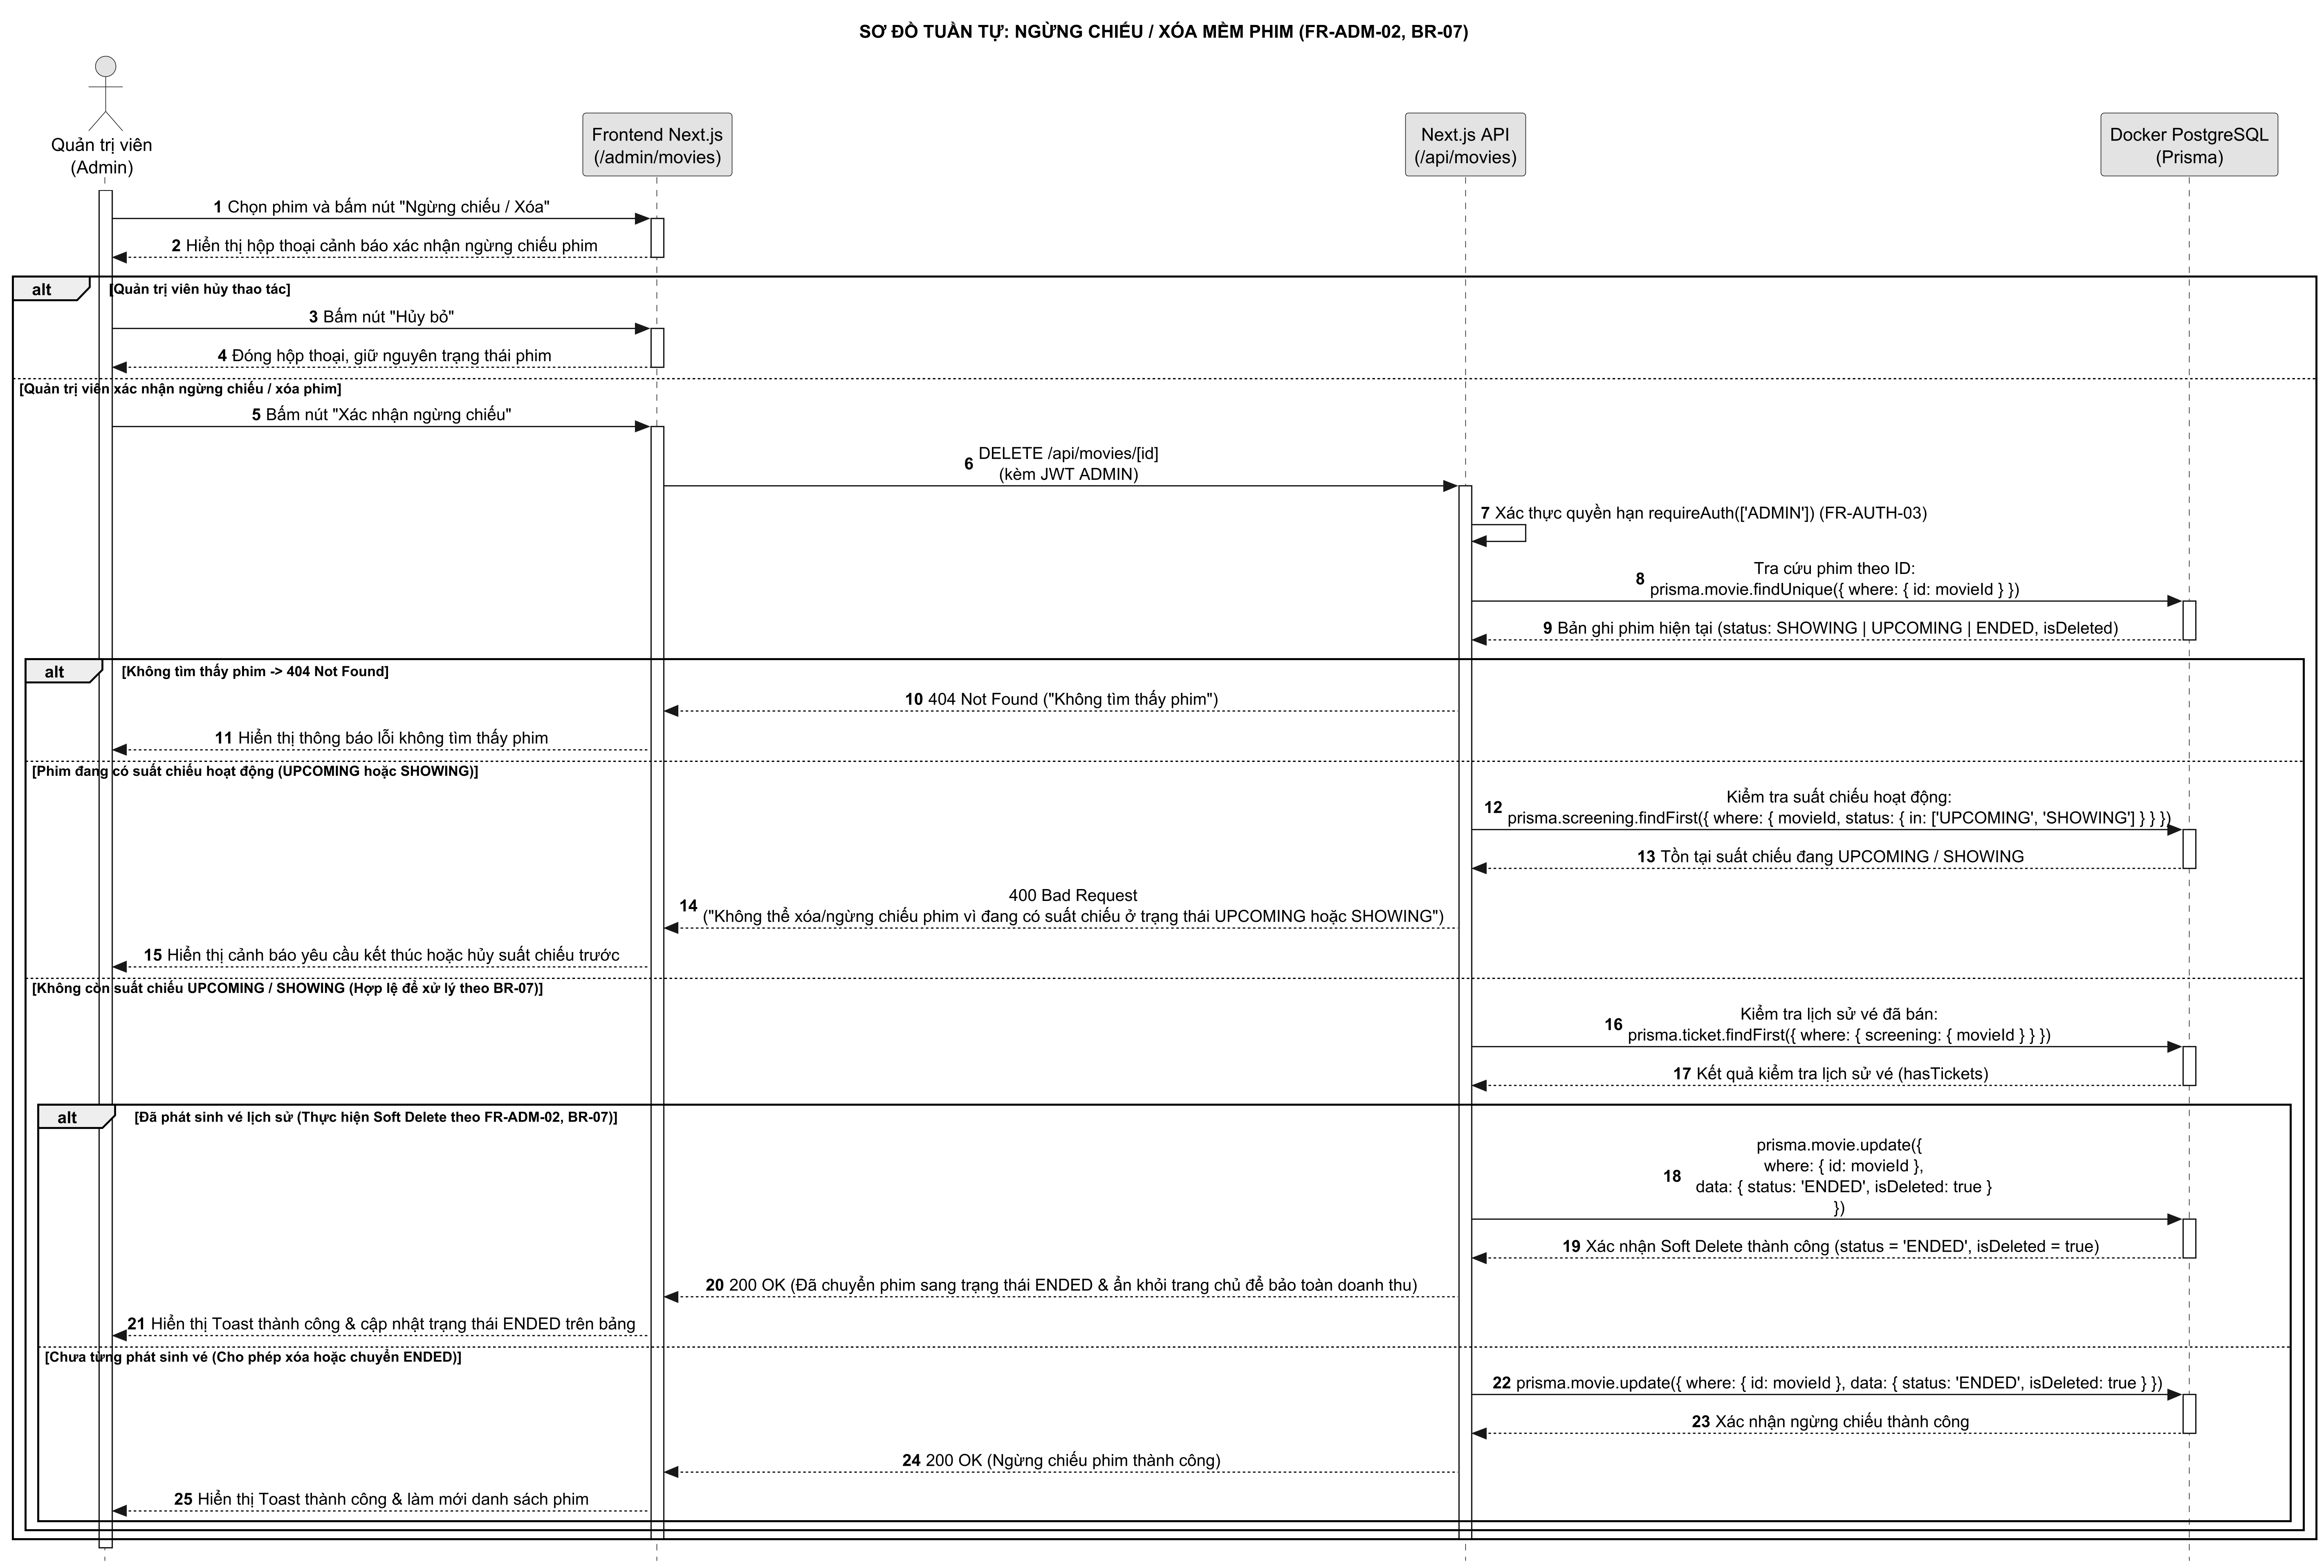
\includegraphics[width=\textwidth,height=0.80\textheight,keepaspectratio]{images/sequence/24_ngung_chieu_phim.png}
  \caption{Sequence Diagram: SƠ ĐỒ TUẦN TỰ: NGỪNG CHIẾU / XÓA MỀM PHIM (FR-ADM-02, BR-07)}
  \label{fig:seq_24}
\end{figure}

\subsection{SƠ ĐỒ TUẦN TỰ: QUẢN TRỊ DANH MỤC COMBO BẮP NƯỚC (TỔNG QUAN)}
\begin{figure}[H]
  \centering
  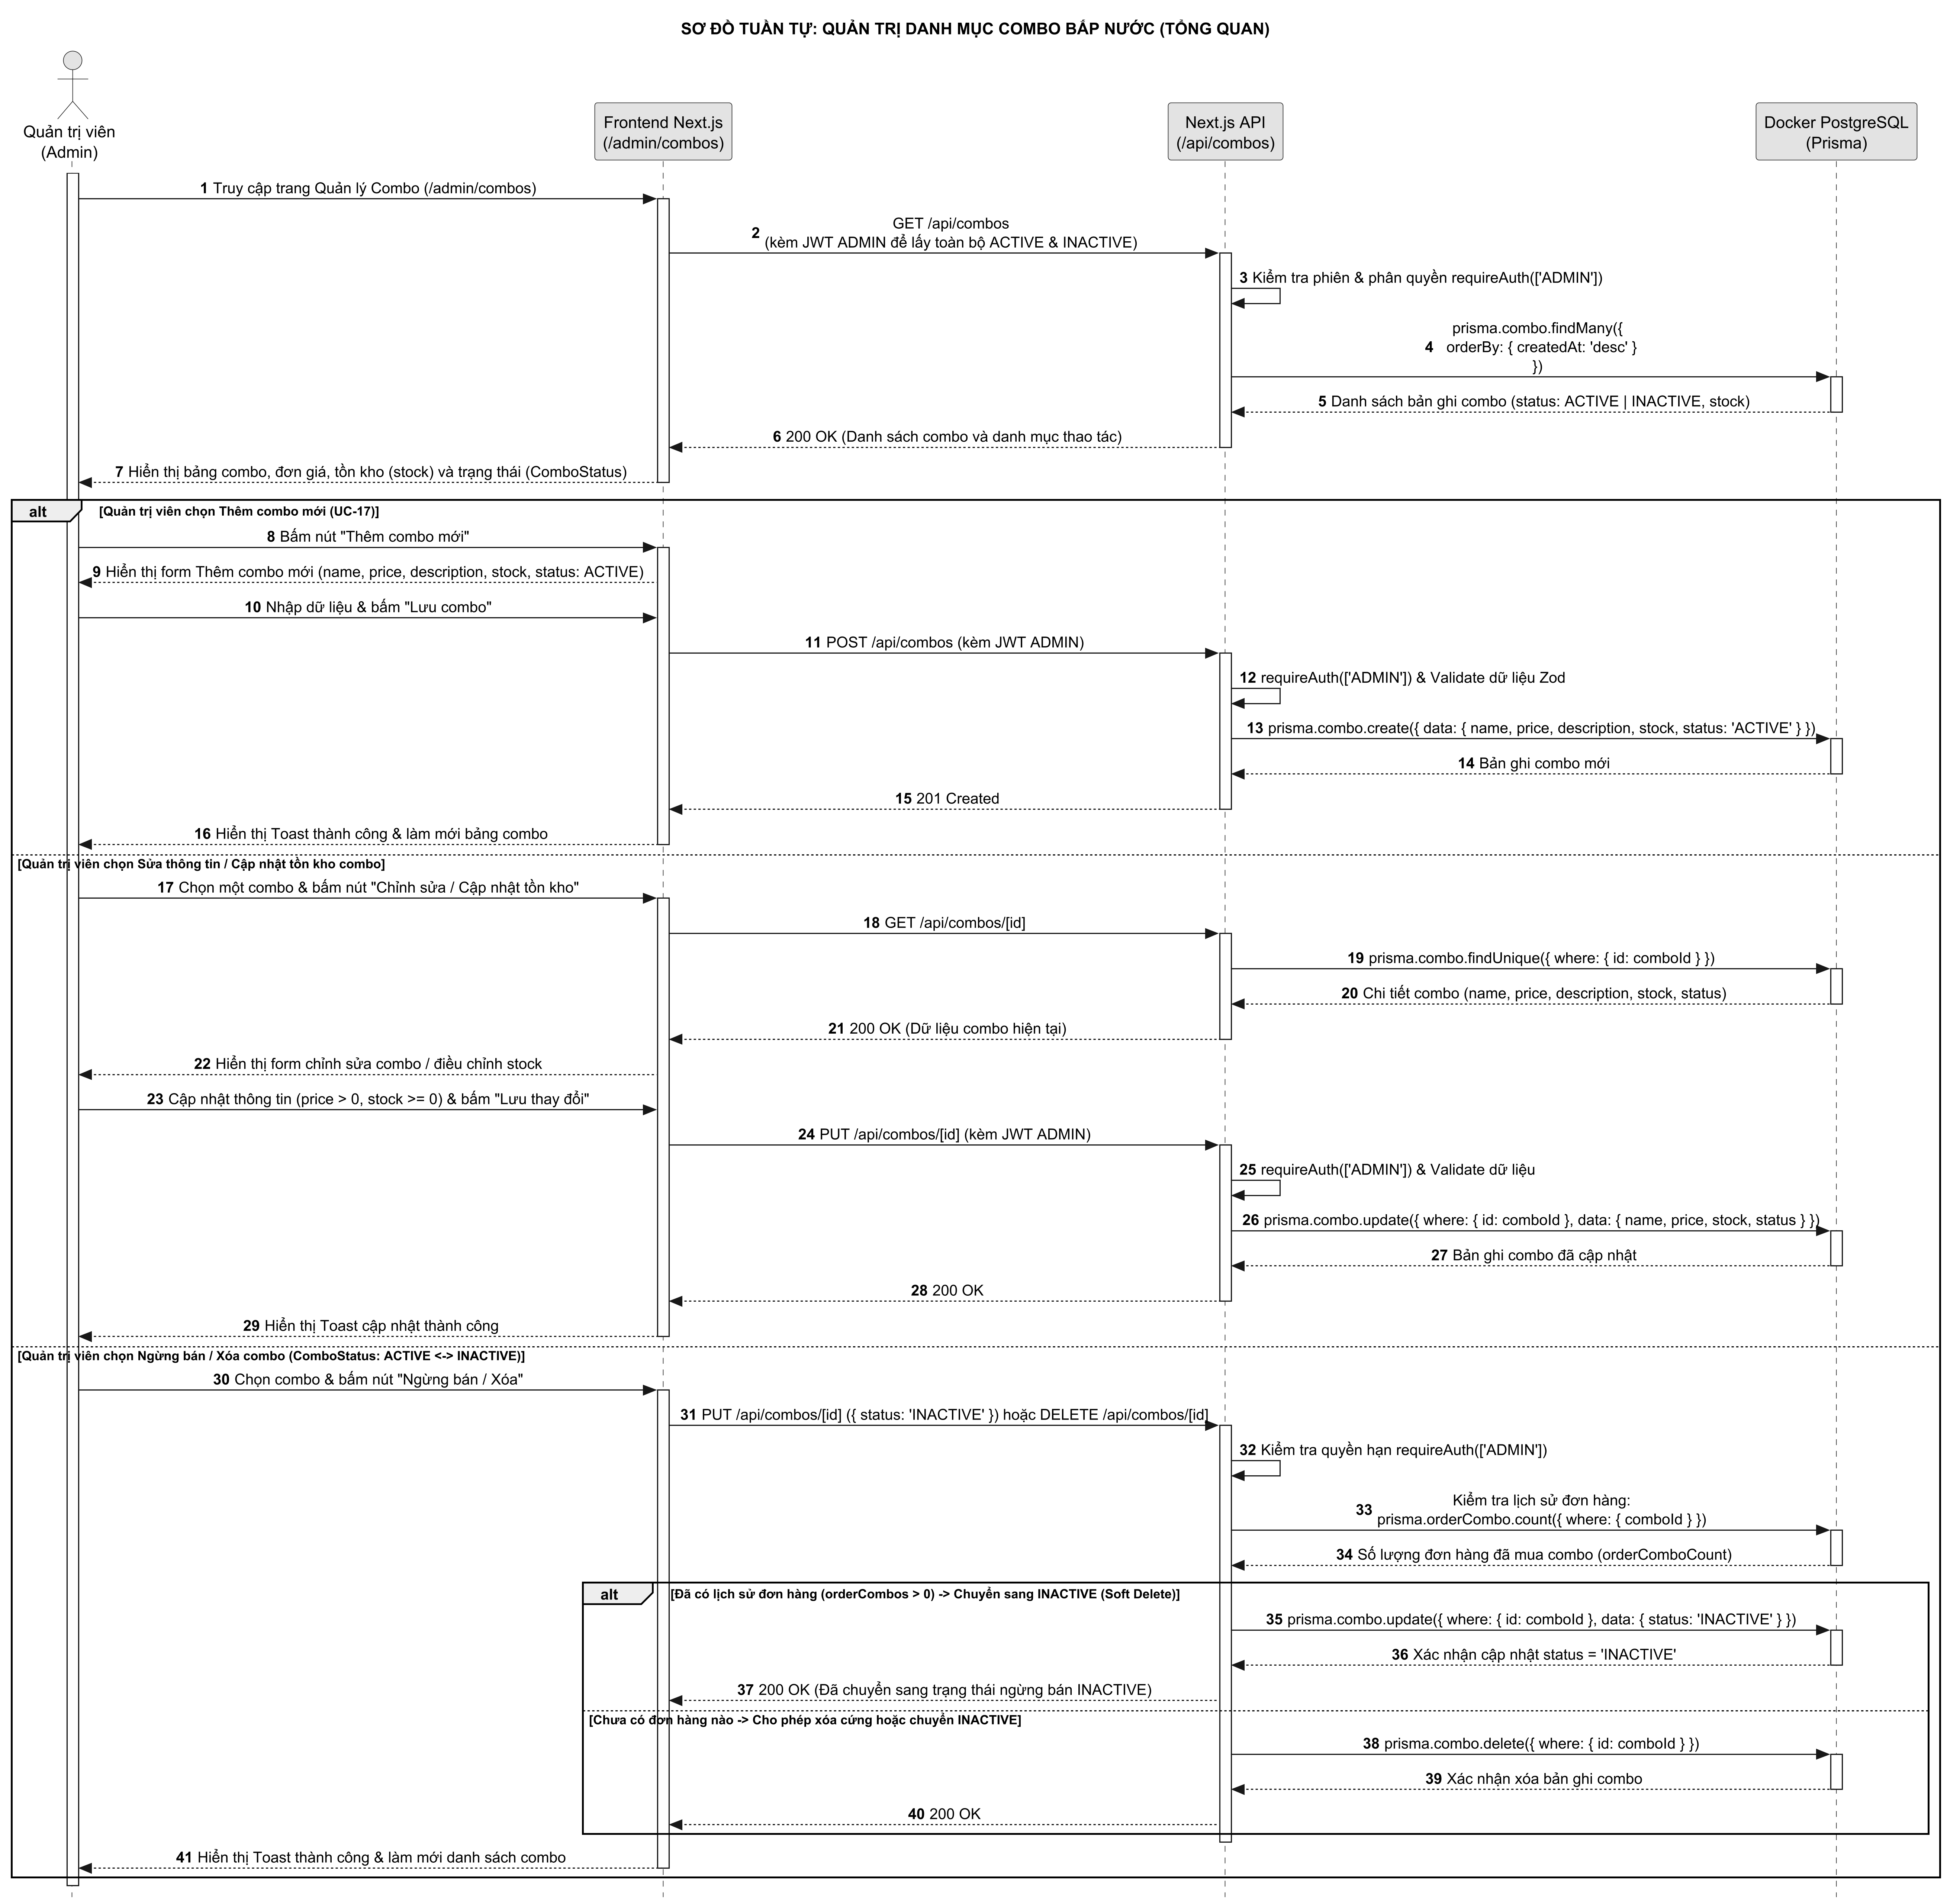
\includegraphics[width=\textwidth,height=0.80\textheight,keepaspectratio]{images/sequence/25_quan_ly_combo_tong_quan.png}
  \caption{Sequence Diagram: SƠ ĐỒ TUẦN TỰ: QUẢN TRỊ DANH MỤC COMBO BẮP NƯỚC (TỔNG QUAN)}
  \label{fig:seq_25}
\end{figure}

\subsection{SƠ ĐỒ TUẦN TỰ: THÊM COMBO MỚI (UC-17)}
\begin{figure}[H]
  \centering
  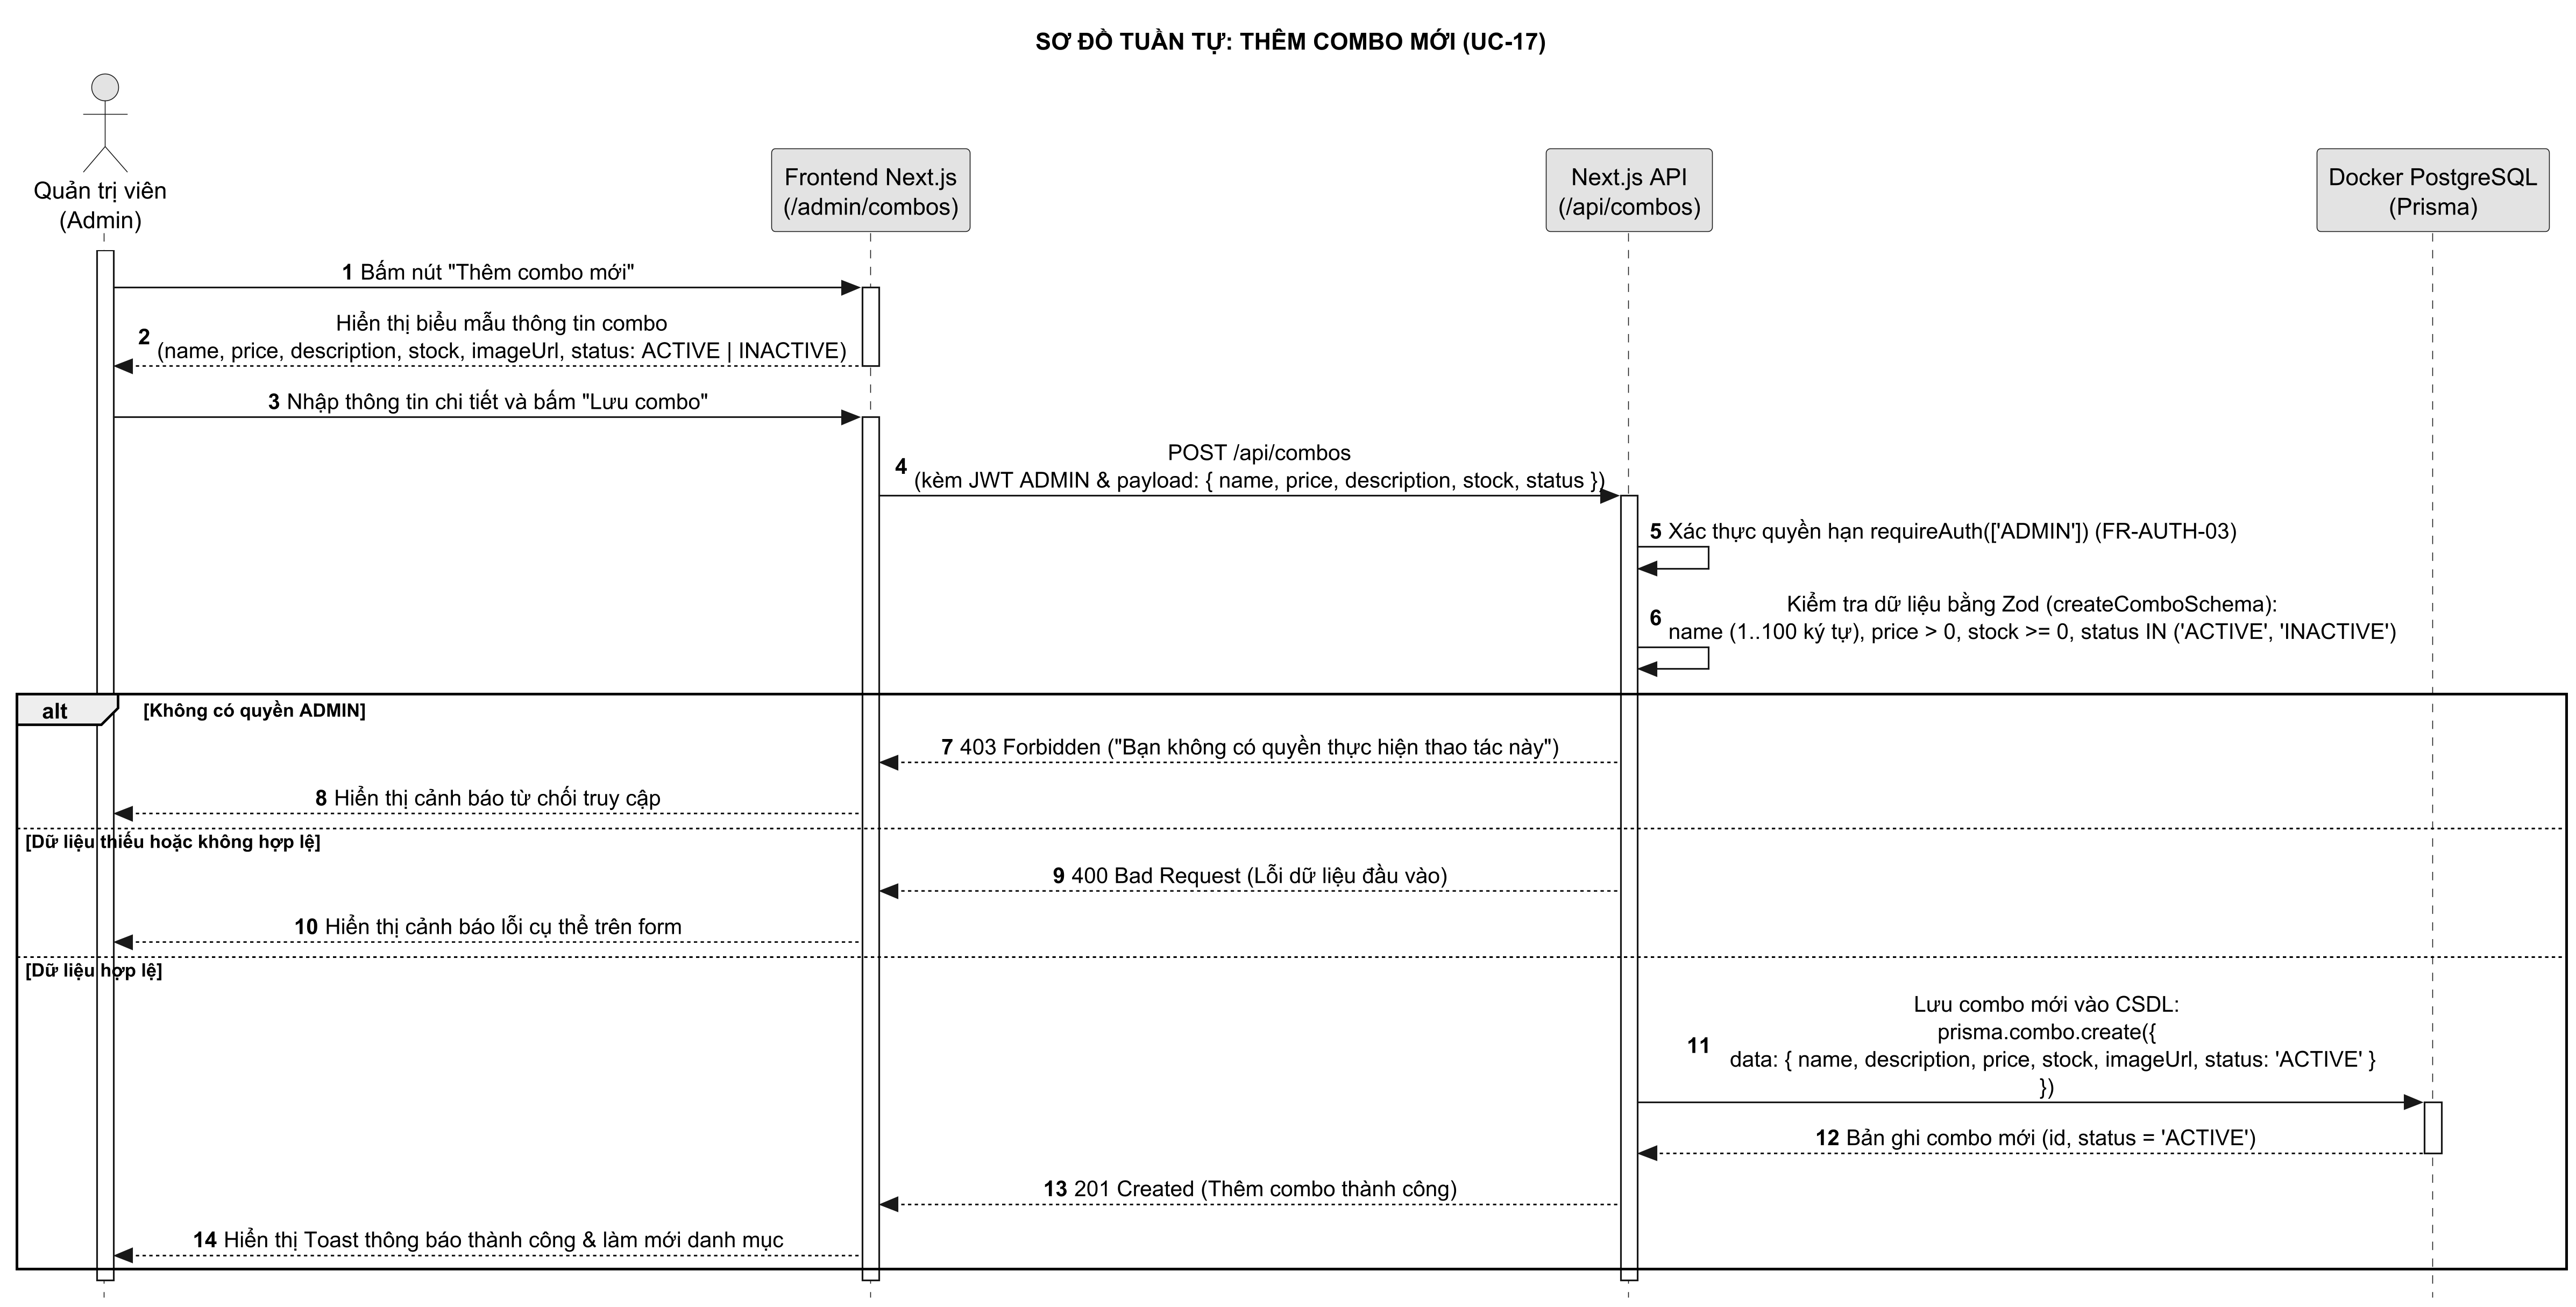
\includegraphics[width=\textwidth,height=0.80\textheight,keepaspectratio]{images/sequence/26_them_combo_moi.png}
  \caption{Sequence Diagram: SƠ ĐỒ TUẦN TỰ: THÊM COMBO MỚI (UC-17)}
  \label{fig:seq_26}
\end{figure}

\subsection{SƠ ĐỒ TUẦN TỰ: CHỈNH SỬA THÔNG TIN COMBO (UC-17)}
\begin{figure}[H]
  \centering
  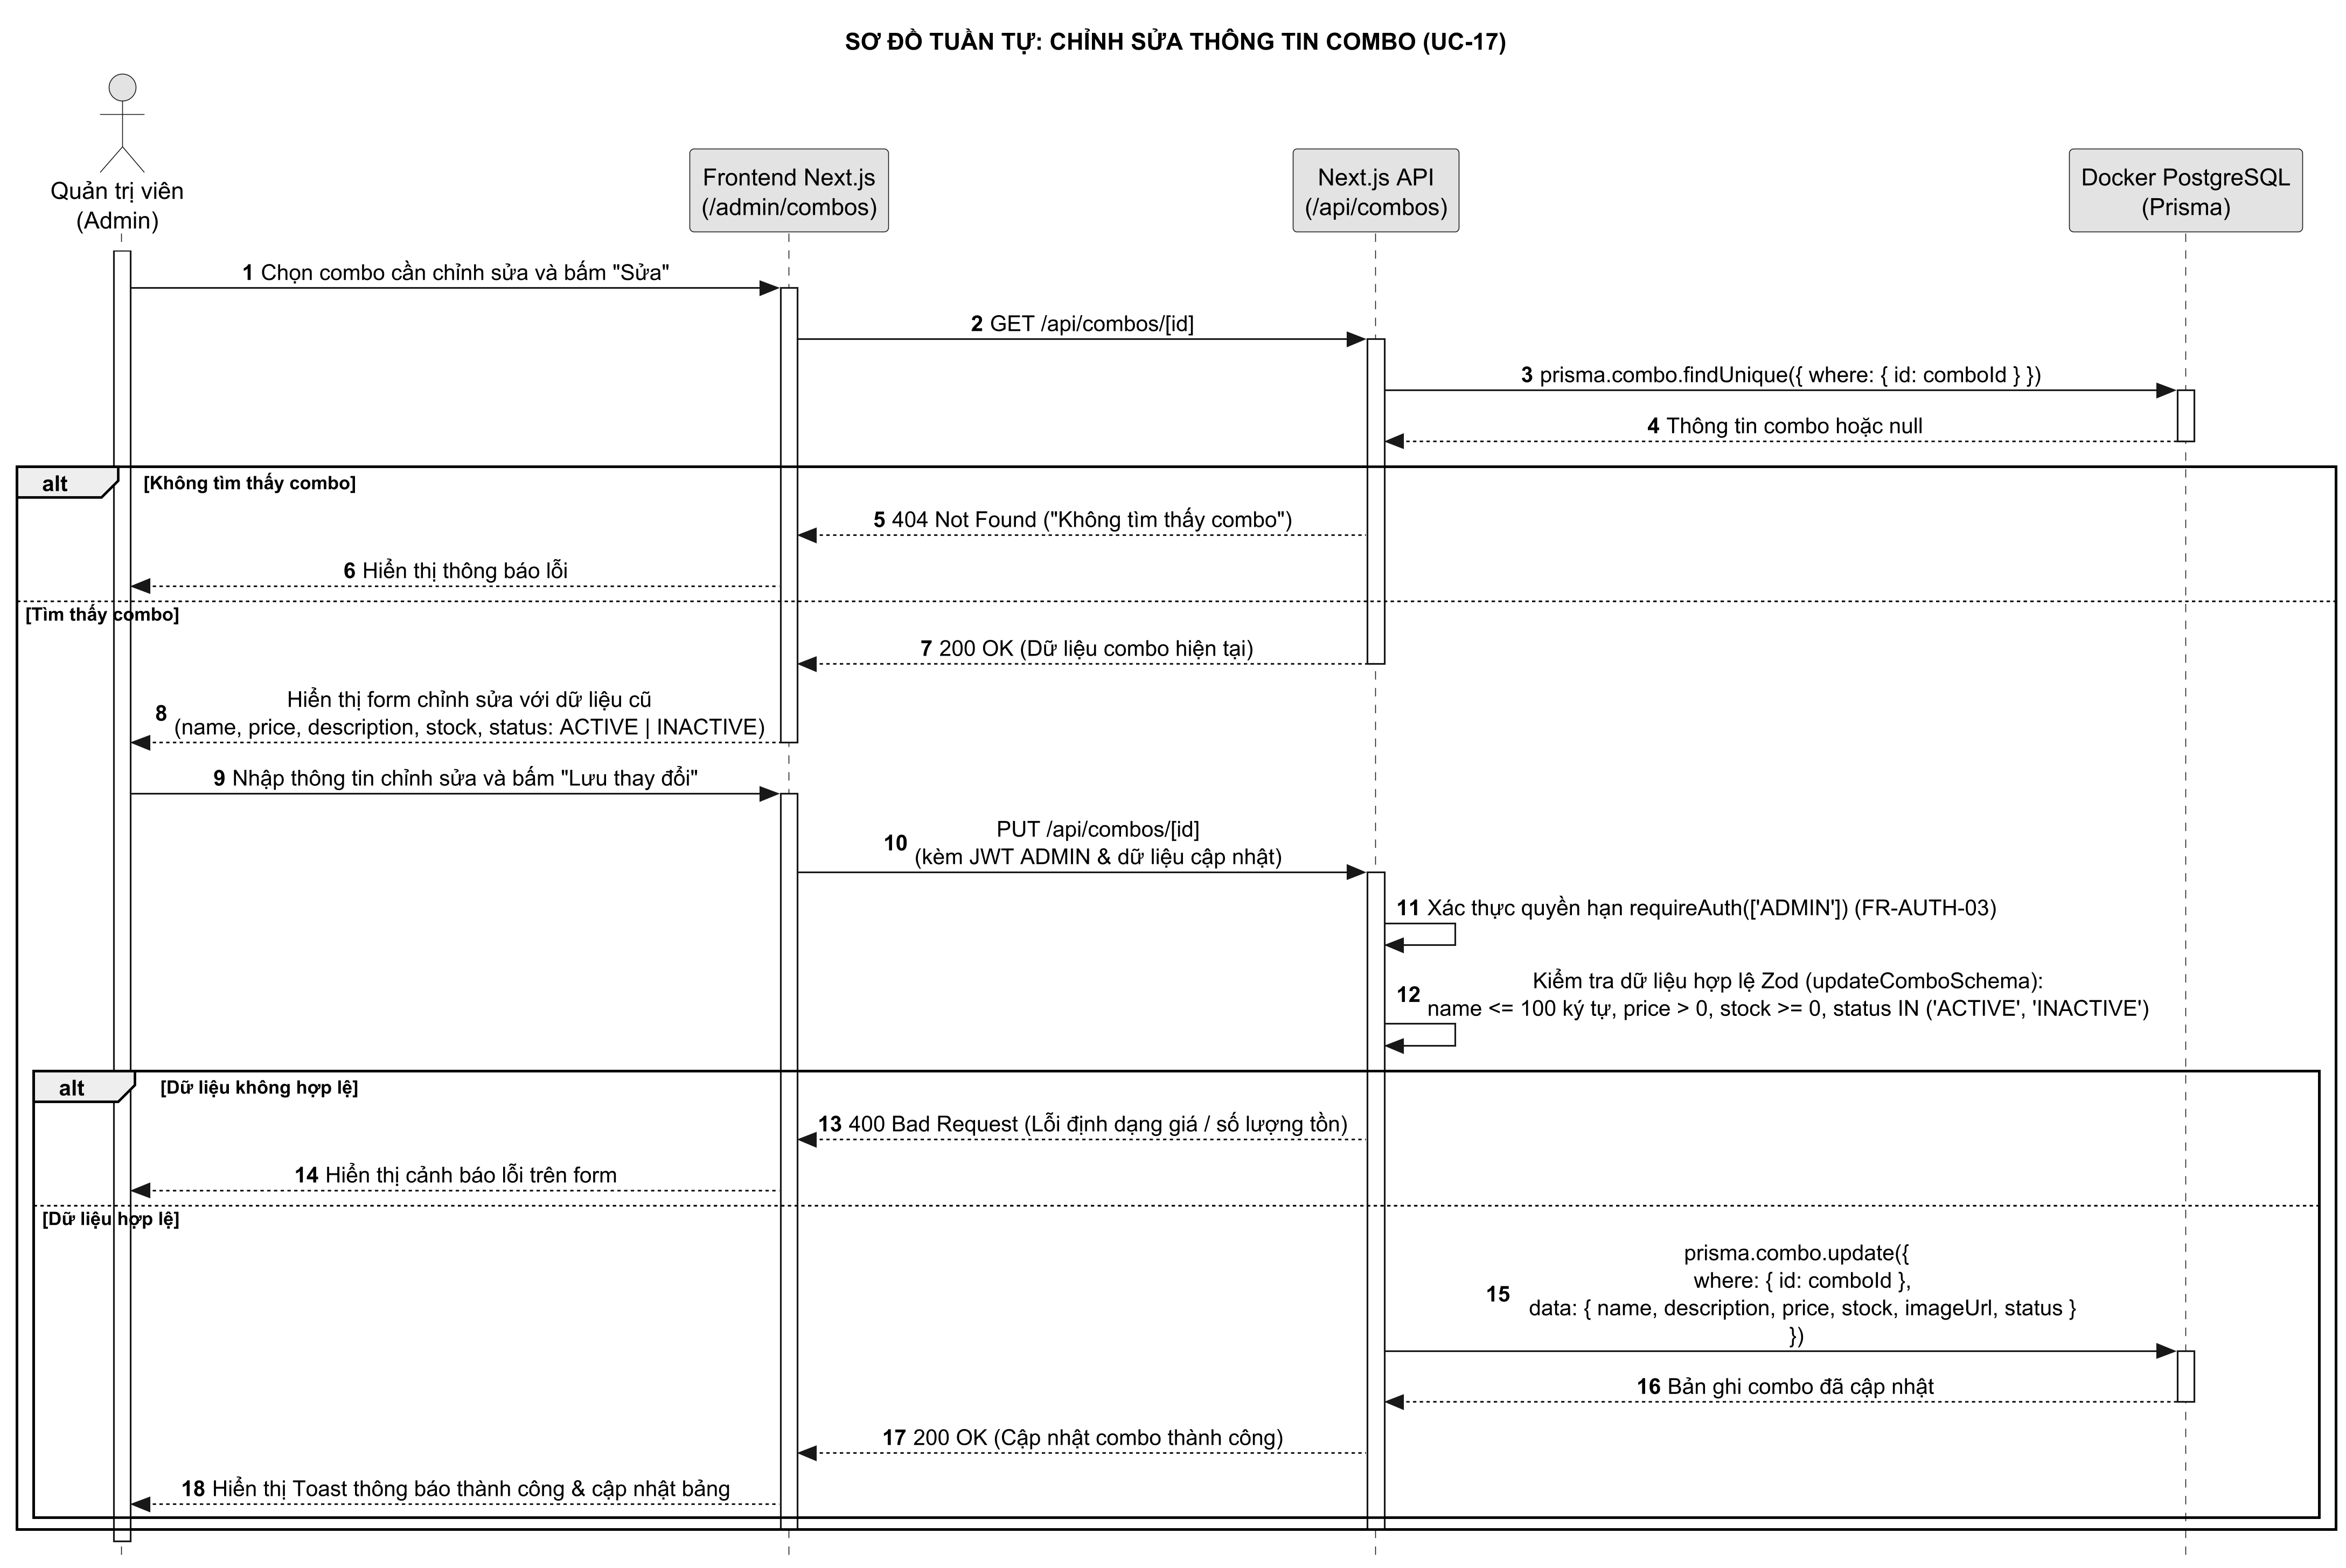
\includegraphics[width=\textwidth,height=0.80\textheight,keepaspectratio]{images/sequence/27_sua_combo.png}
  \caption{Sequence Diagram: SƠ ĐỒ TUẦN TỰ: CHỈNH SỬA THÔNG TIN COMBO (UC-17)}
  \label{fig:seq_27}
\end{figure}

\subsection{SƠ ĐỒ TUẦN TỰ: NGỪNG BÁN / XÓA COMBO BẮP NƯỚC (UC-17)}
\begin{figure}[H]
  \centering
  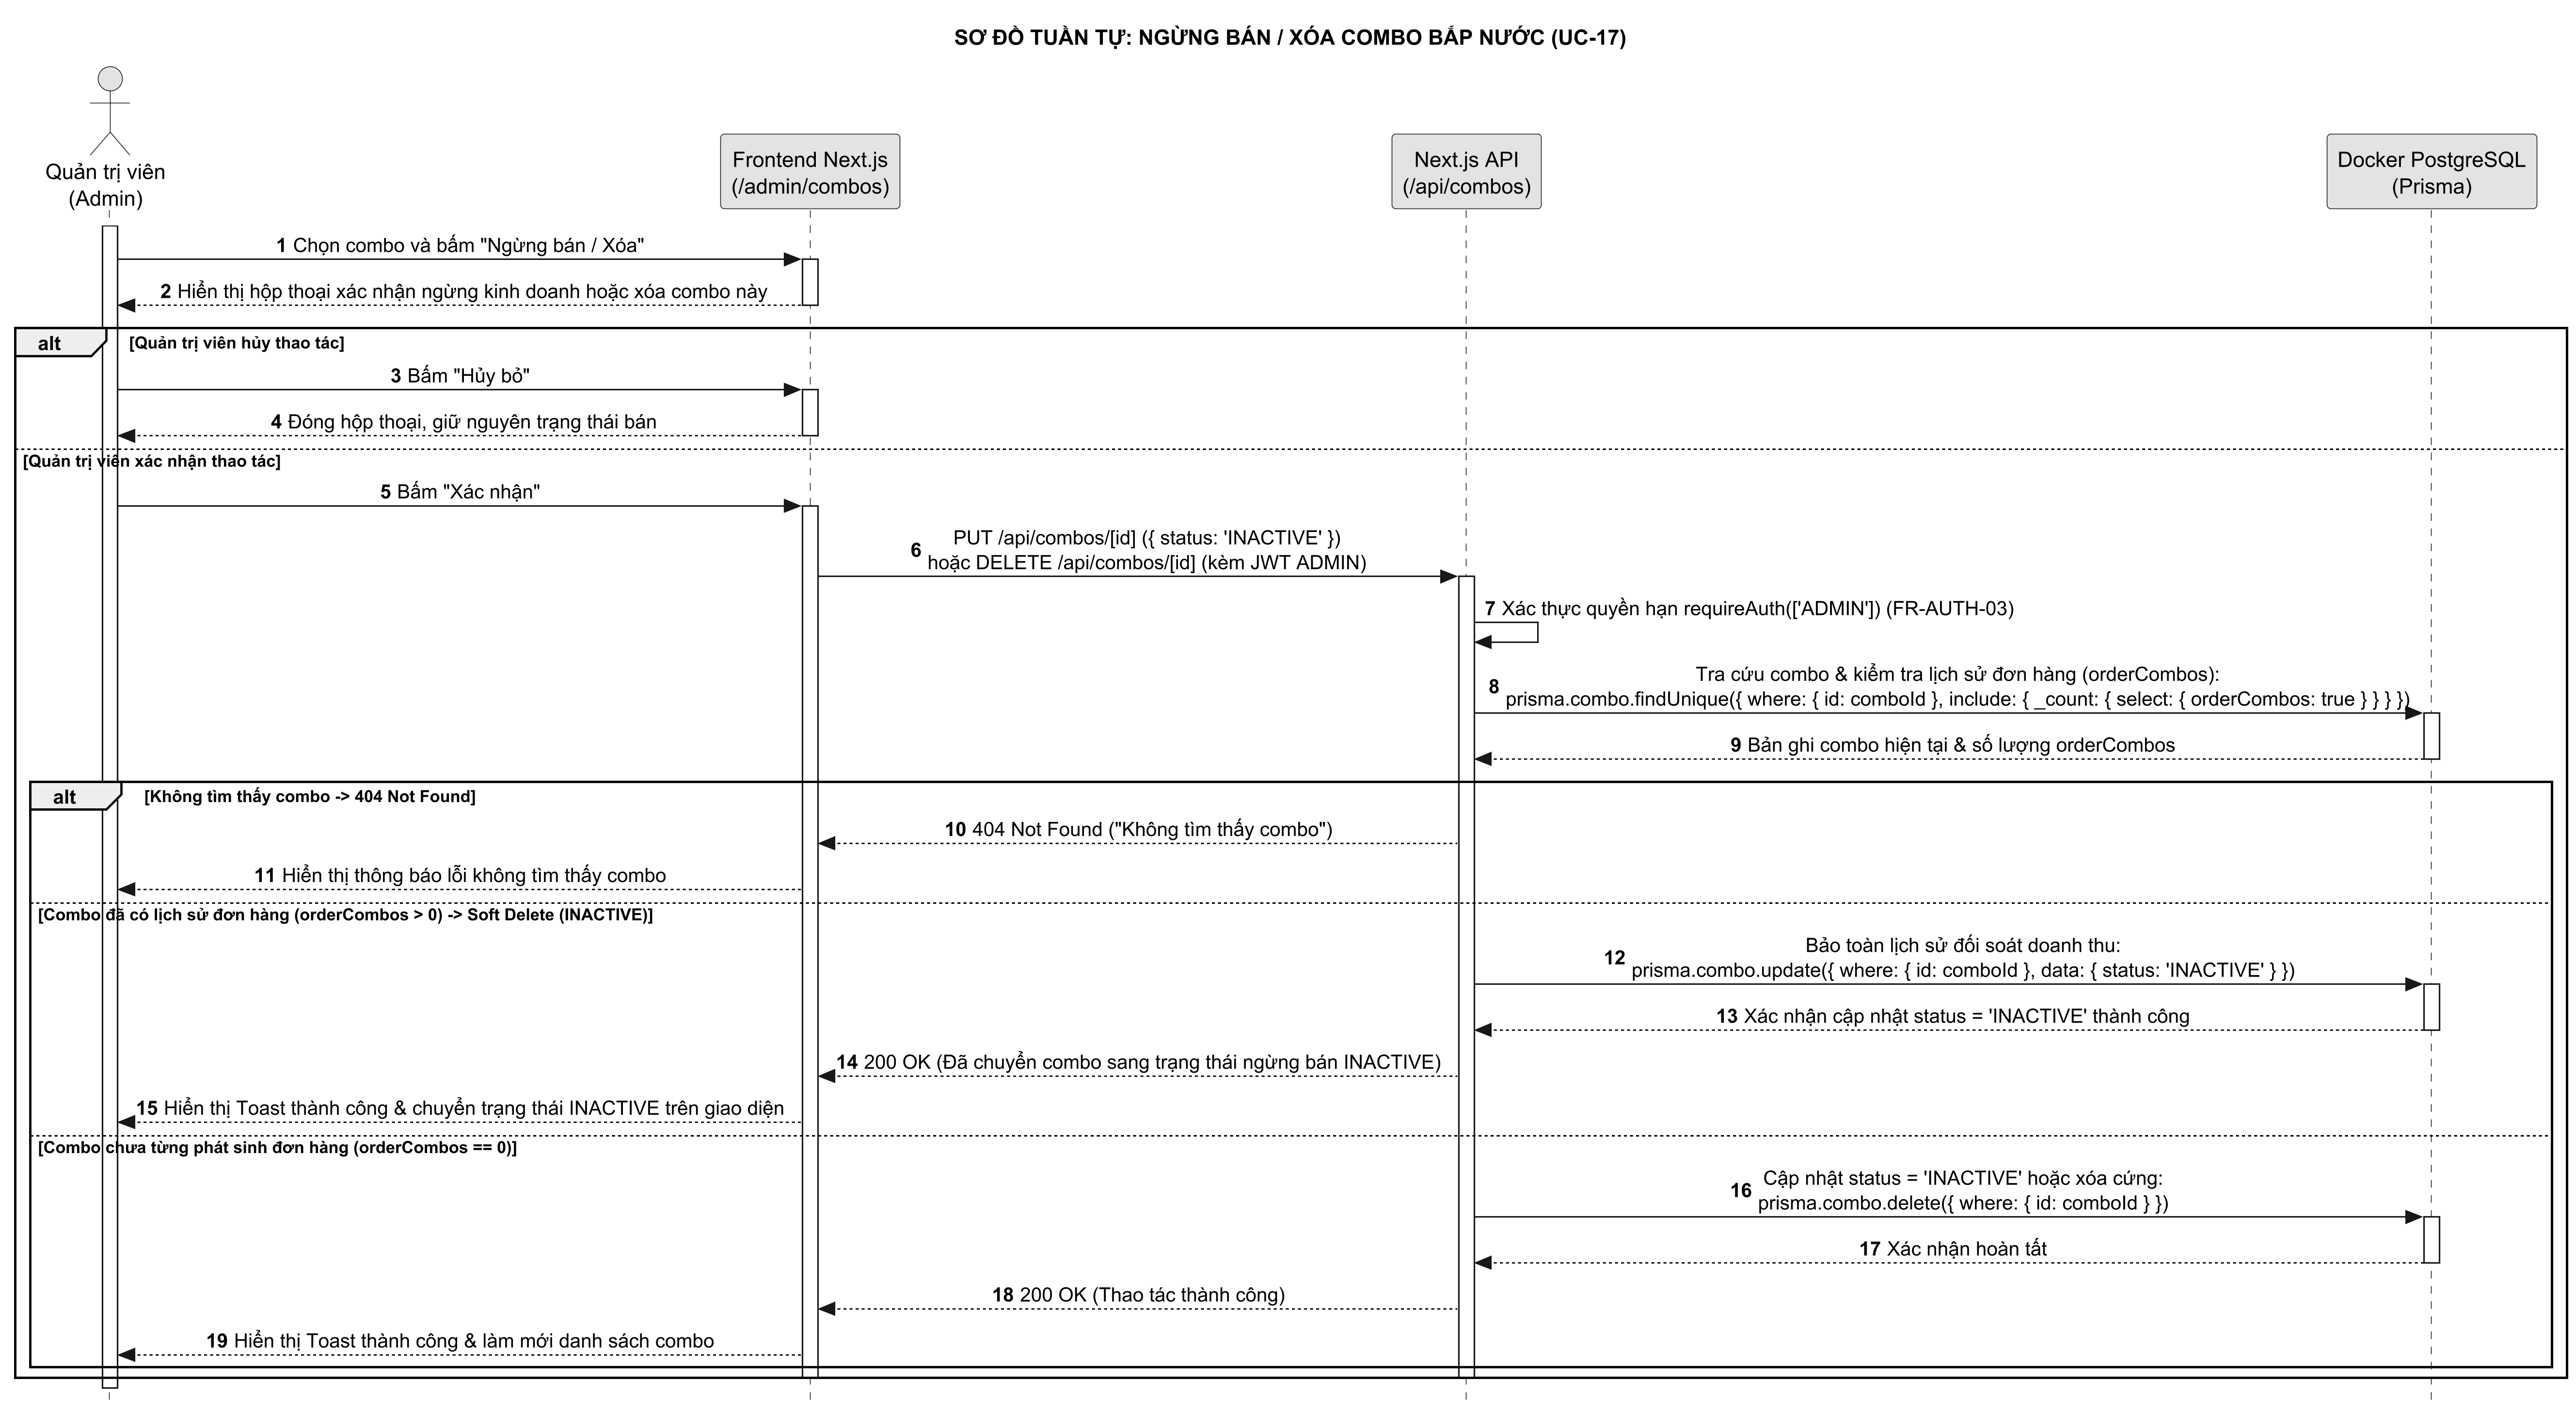
\includegraphics[width=\textwidth,height=0.80\textheight,keepaspectratio]{images/sequence/28_ngung_ban_combo.png}
  \caption{Sequence Diagram: SƠ ĐỒ TUẦN TỰ: NGỪNG BÁN / XÓA COMBO BẮP NƯỚC (UC-17)}
  \label{fig:seq_28}
\end{figure}

\subsection{SƠ ĐỒ TUẦN TỰ: CẬP NHẬT TỒN KHO COMBO (UC-17)}
\begin{figure}[H]
  \centering
  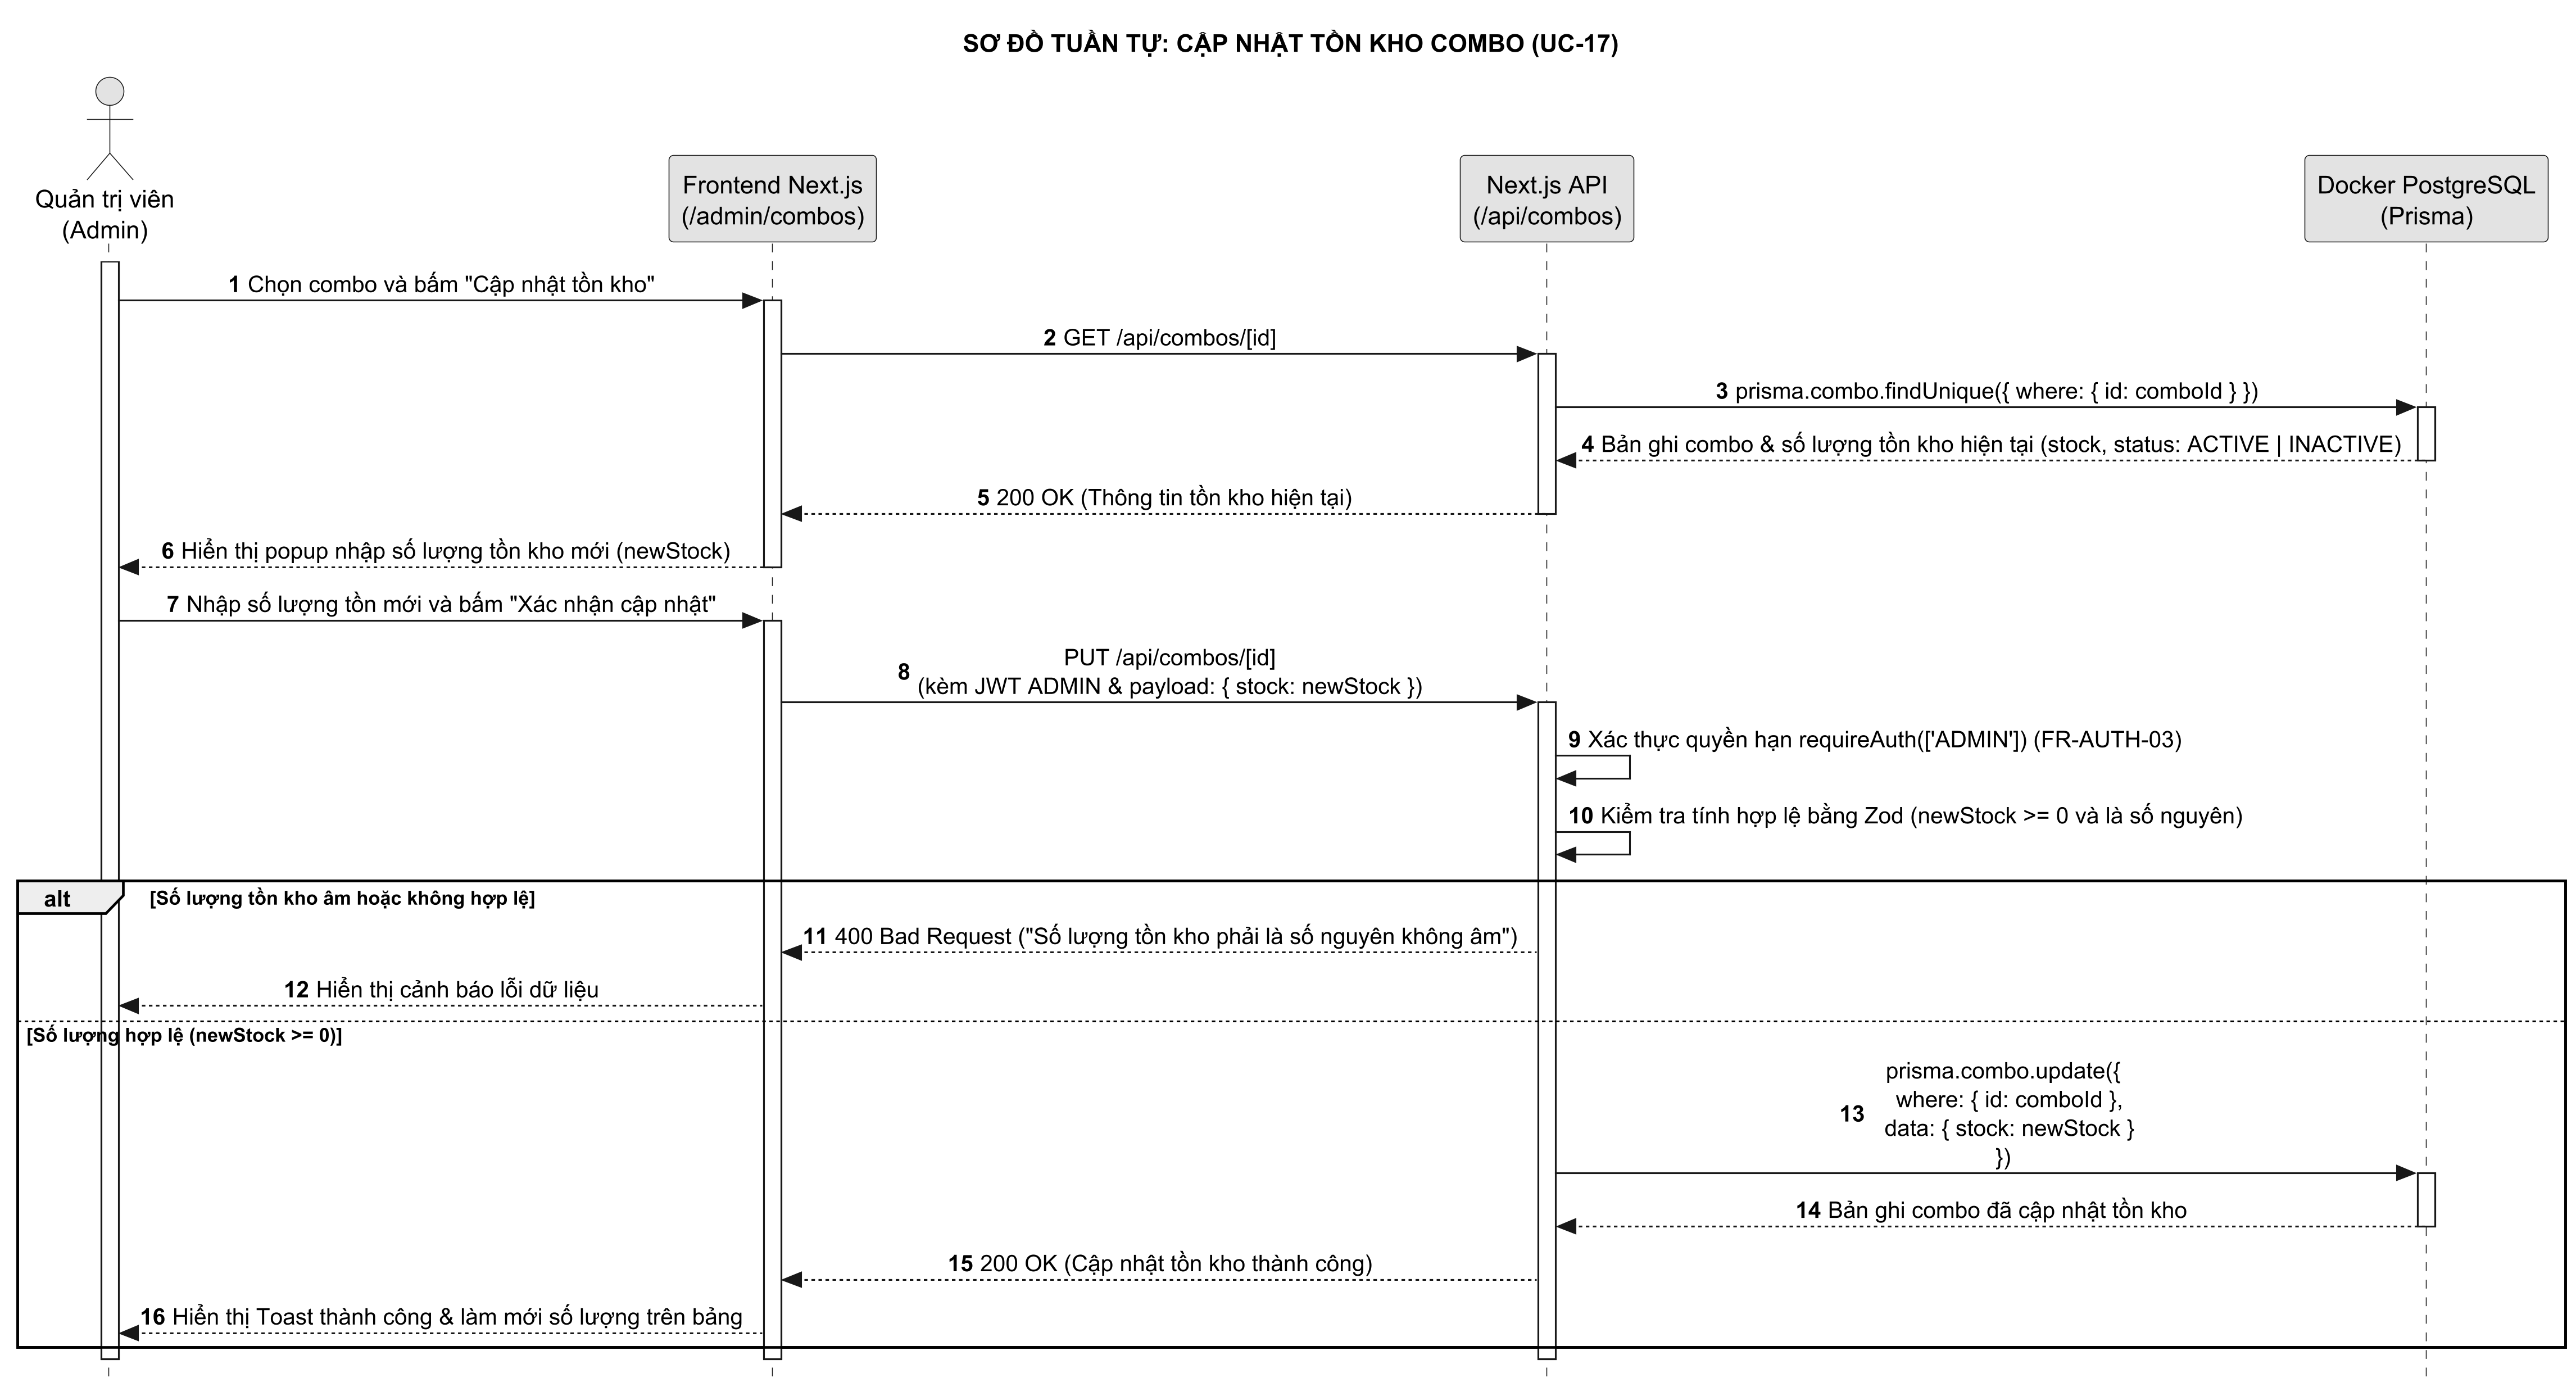
\includegraphics[width=\textwidth,height=0.80\textheight,keepaspectratio]{images/sequence/29_cap_nhat_ton_kho_combo.png}
  \caption{Sequence Diagram: SƠ ĐỒ TUẦN TỰ: CẬP NHẬT TỒN KHO COMBO (UC-17)}
  \label{fig:seq_29}
\end{figure}

\subsection{SƠ ĐỒ TUẦN TỰ: QUẢN TRỊ VOUCHER KHUYẾN MÃI (TỔNG QUAN - FR-VOU-01, BR-03)}
\begin{figure}[H]
  \centering
  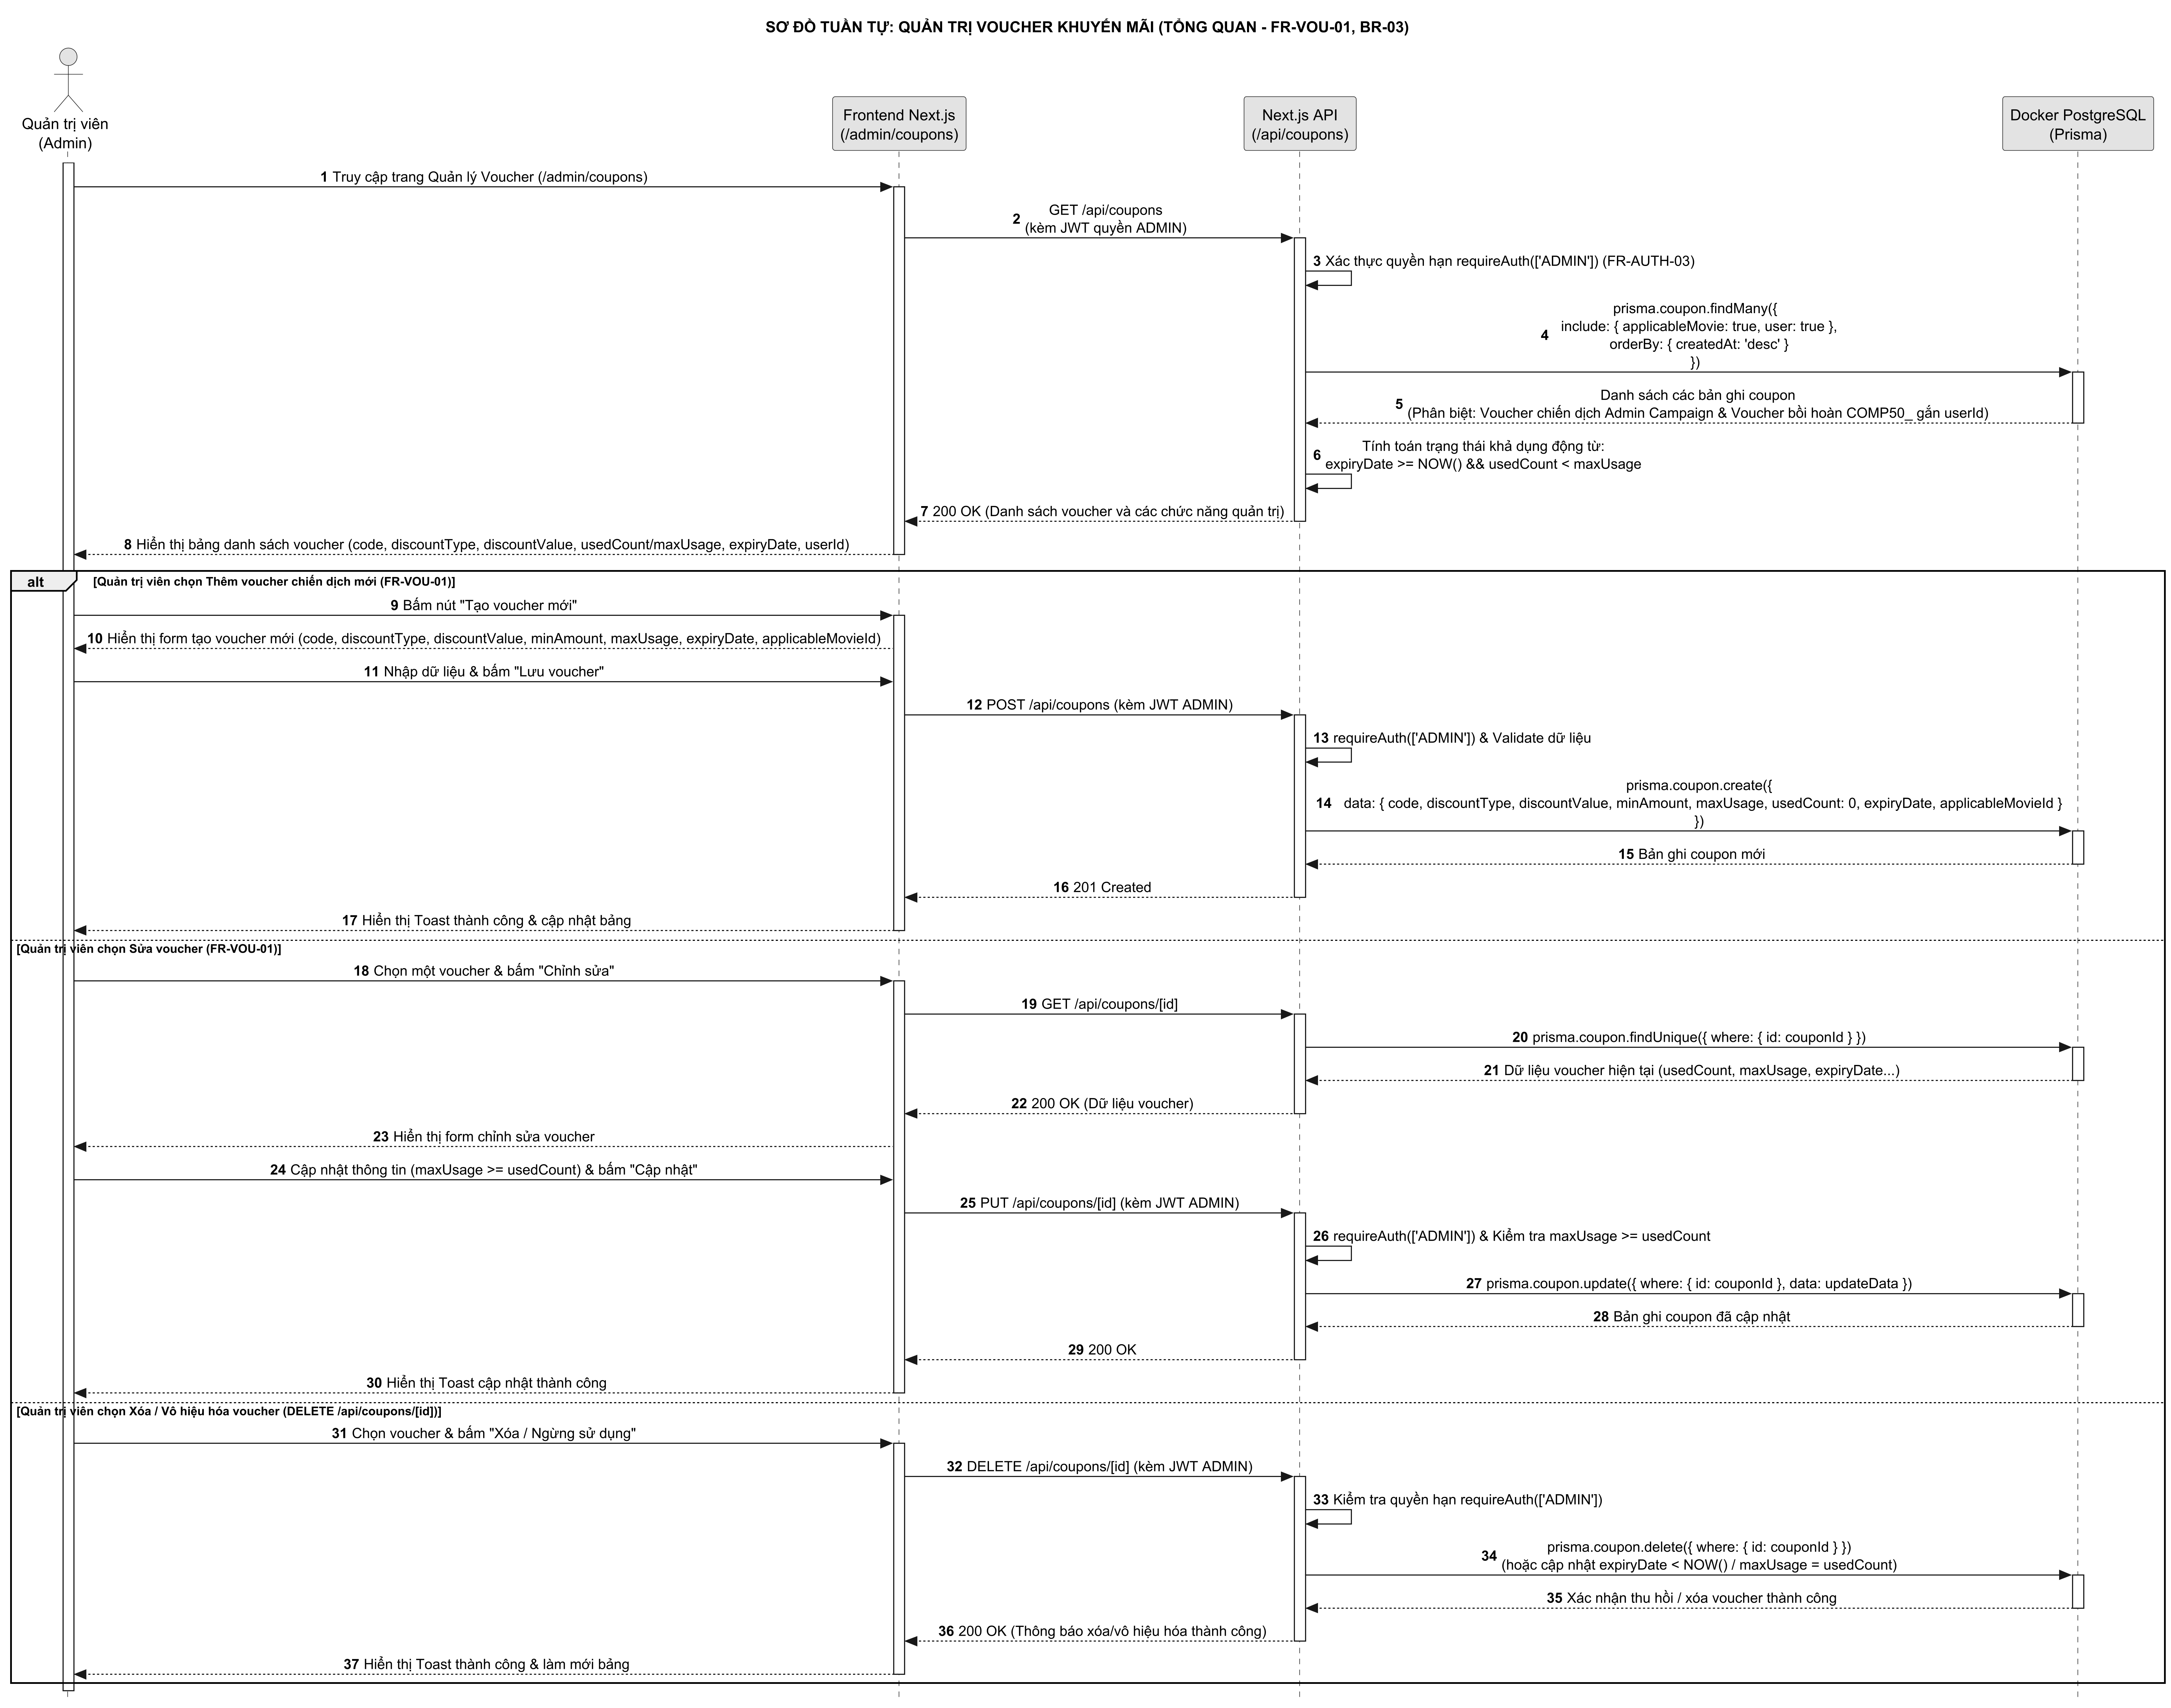
\includegraphics[width=\textwidth,height=0.80\textheight,keepaspectratio]{images/sequence/30_quan_ly_voucher_tong_quan.png}
  \caption{Sequence Diagram: SƠ ĐỒ TUẦN TỰ: QUẢN TRỊ VOUCHER KHUYẾN MÃI (TỔNG QUAN - FR-VOU-01, BR-03)}
  \label{fig:seq_30}
\end{figure}

\subsection{SƠ ĐỒ TUẦN TỰ: THÊM VOUCHER MỚI (FR-VOU-01)}
\begin{figure}[H]
  \centering
  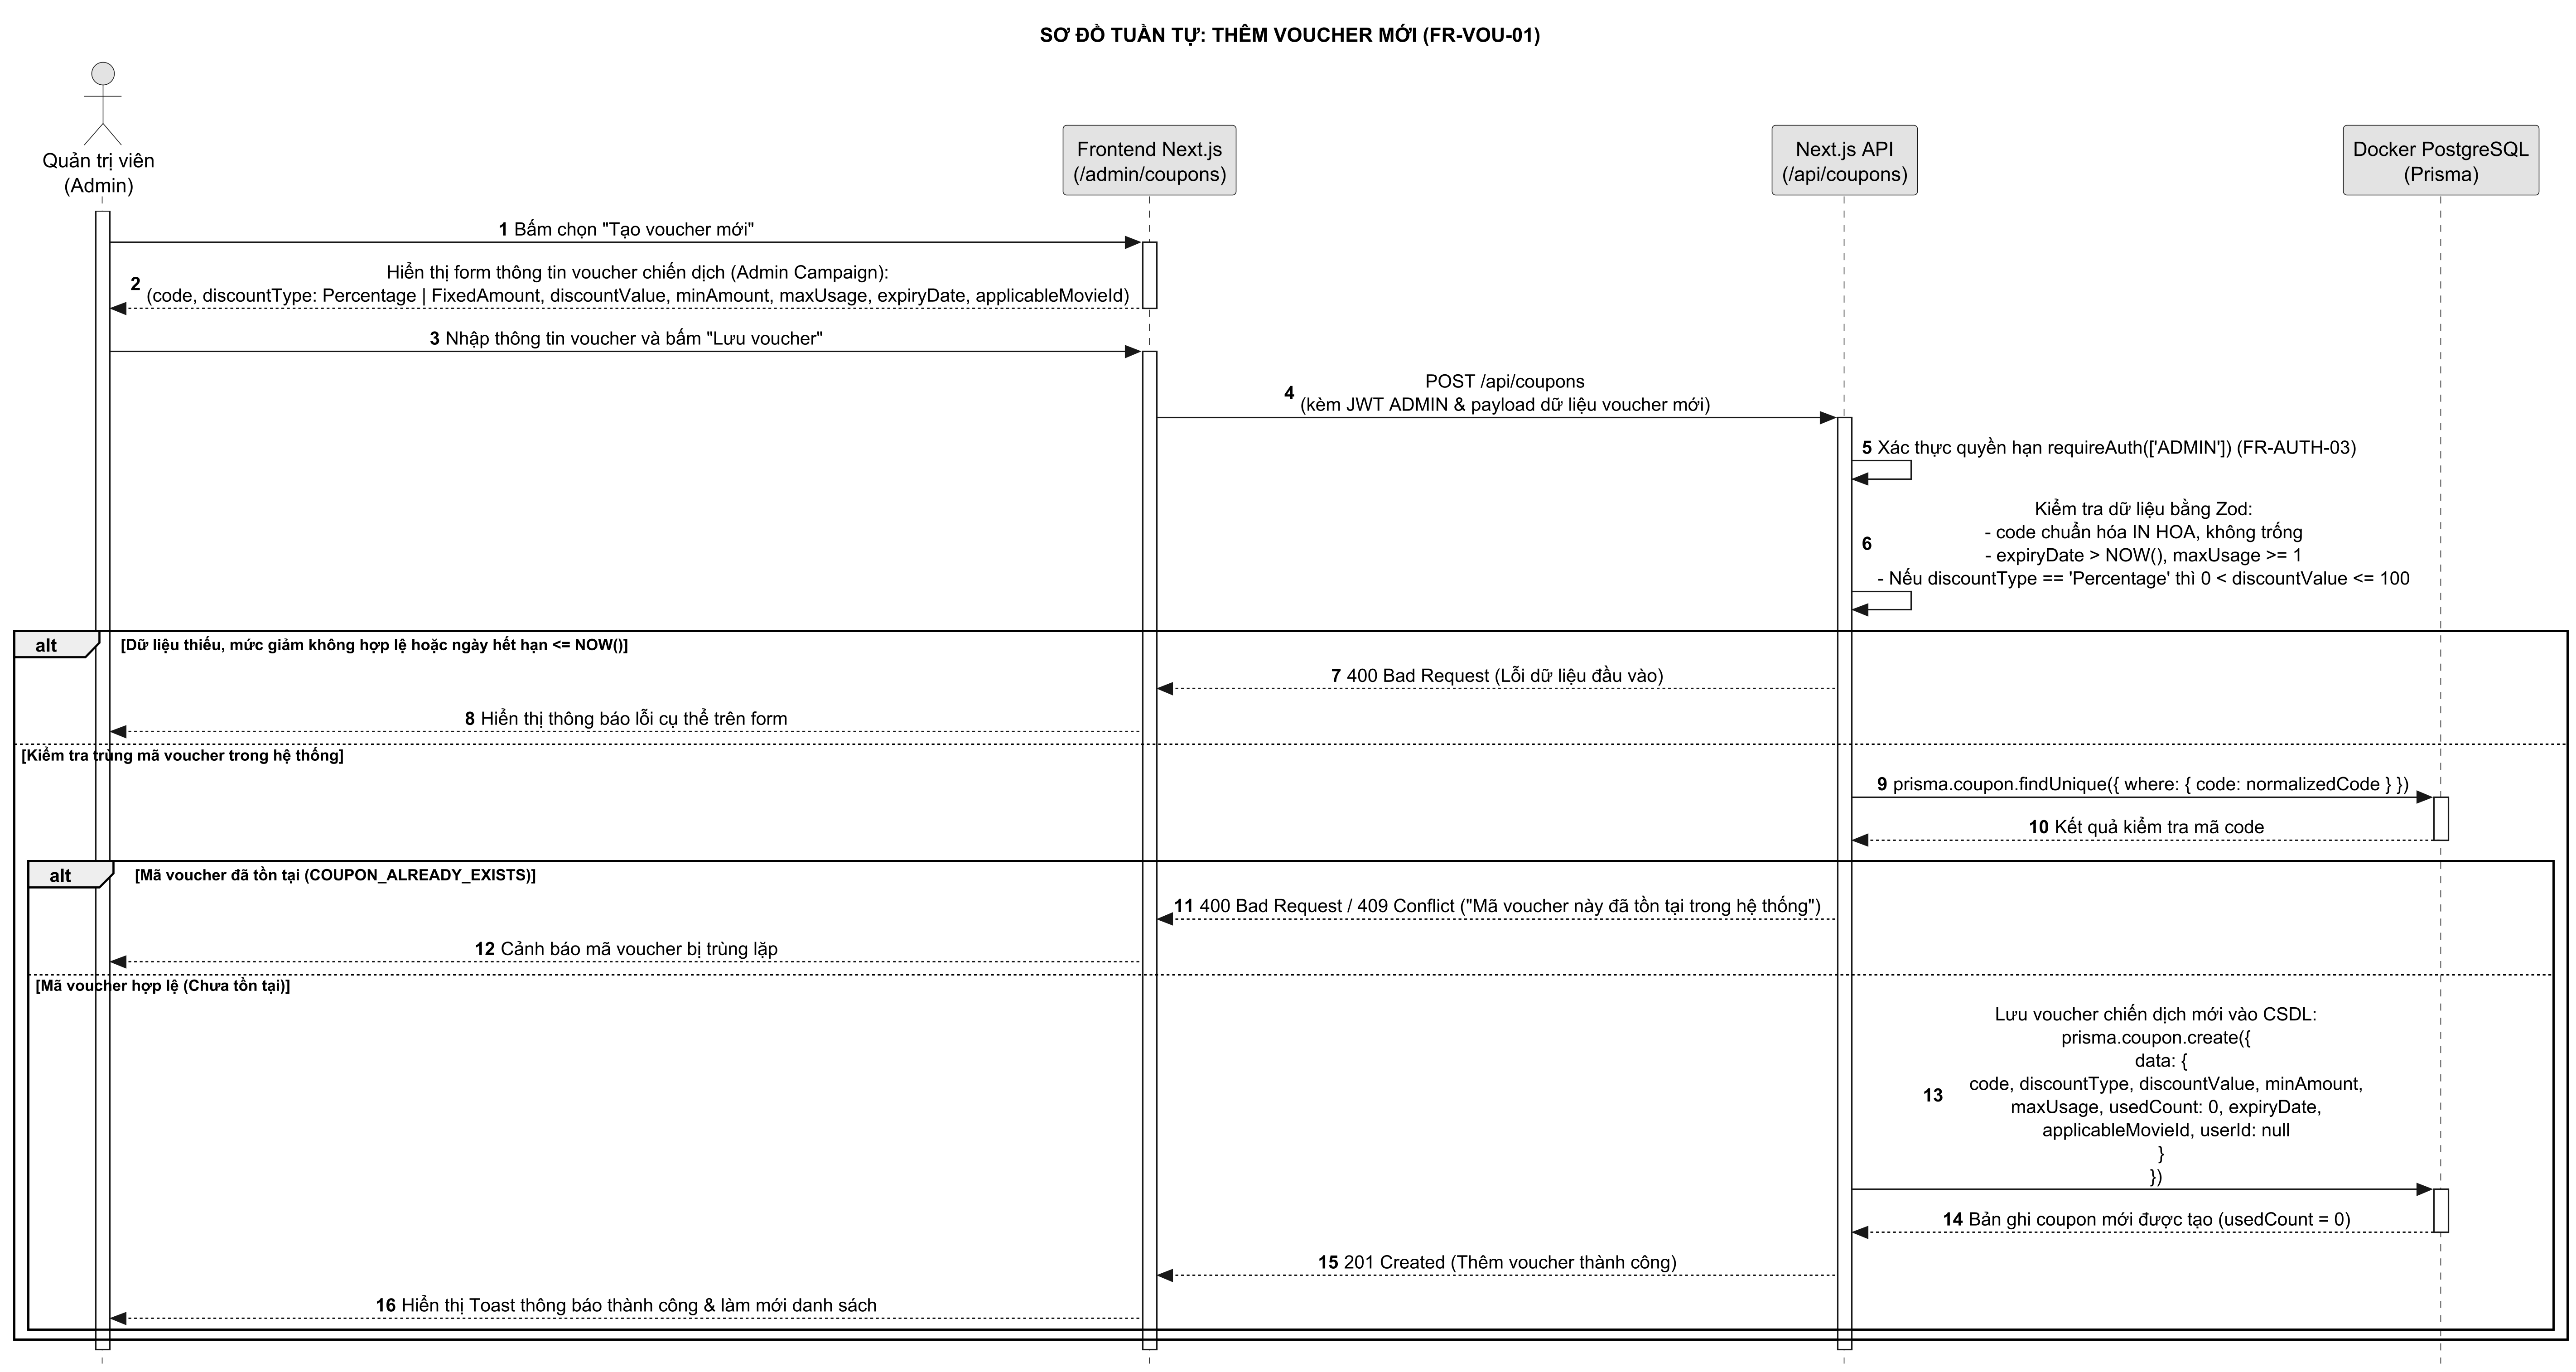
\includegraphics[width=\textwidth,height=0.80\textheight,keepaspectratio]{images/sequence/31_them_voucher.png}
  \caption{Sequence Diagram: SƠ ĐỒ TUẦN TỰ: THÊM VOUCHER MỚI (FR-VOU-01)}
  \label{fig:seq_31}
\end{figure}

\subsection{SƠ ĐỒ TUẦN TỰ: CHỈNH SỬA VOUCHER (FR-VOU-01)}
\begin{figure}[H]
  \centering
  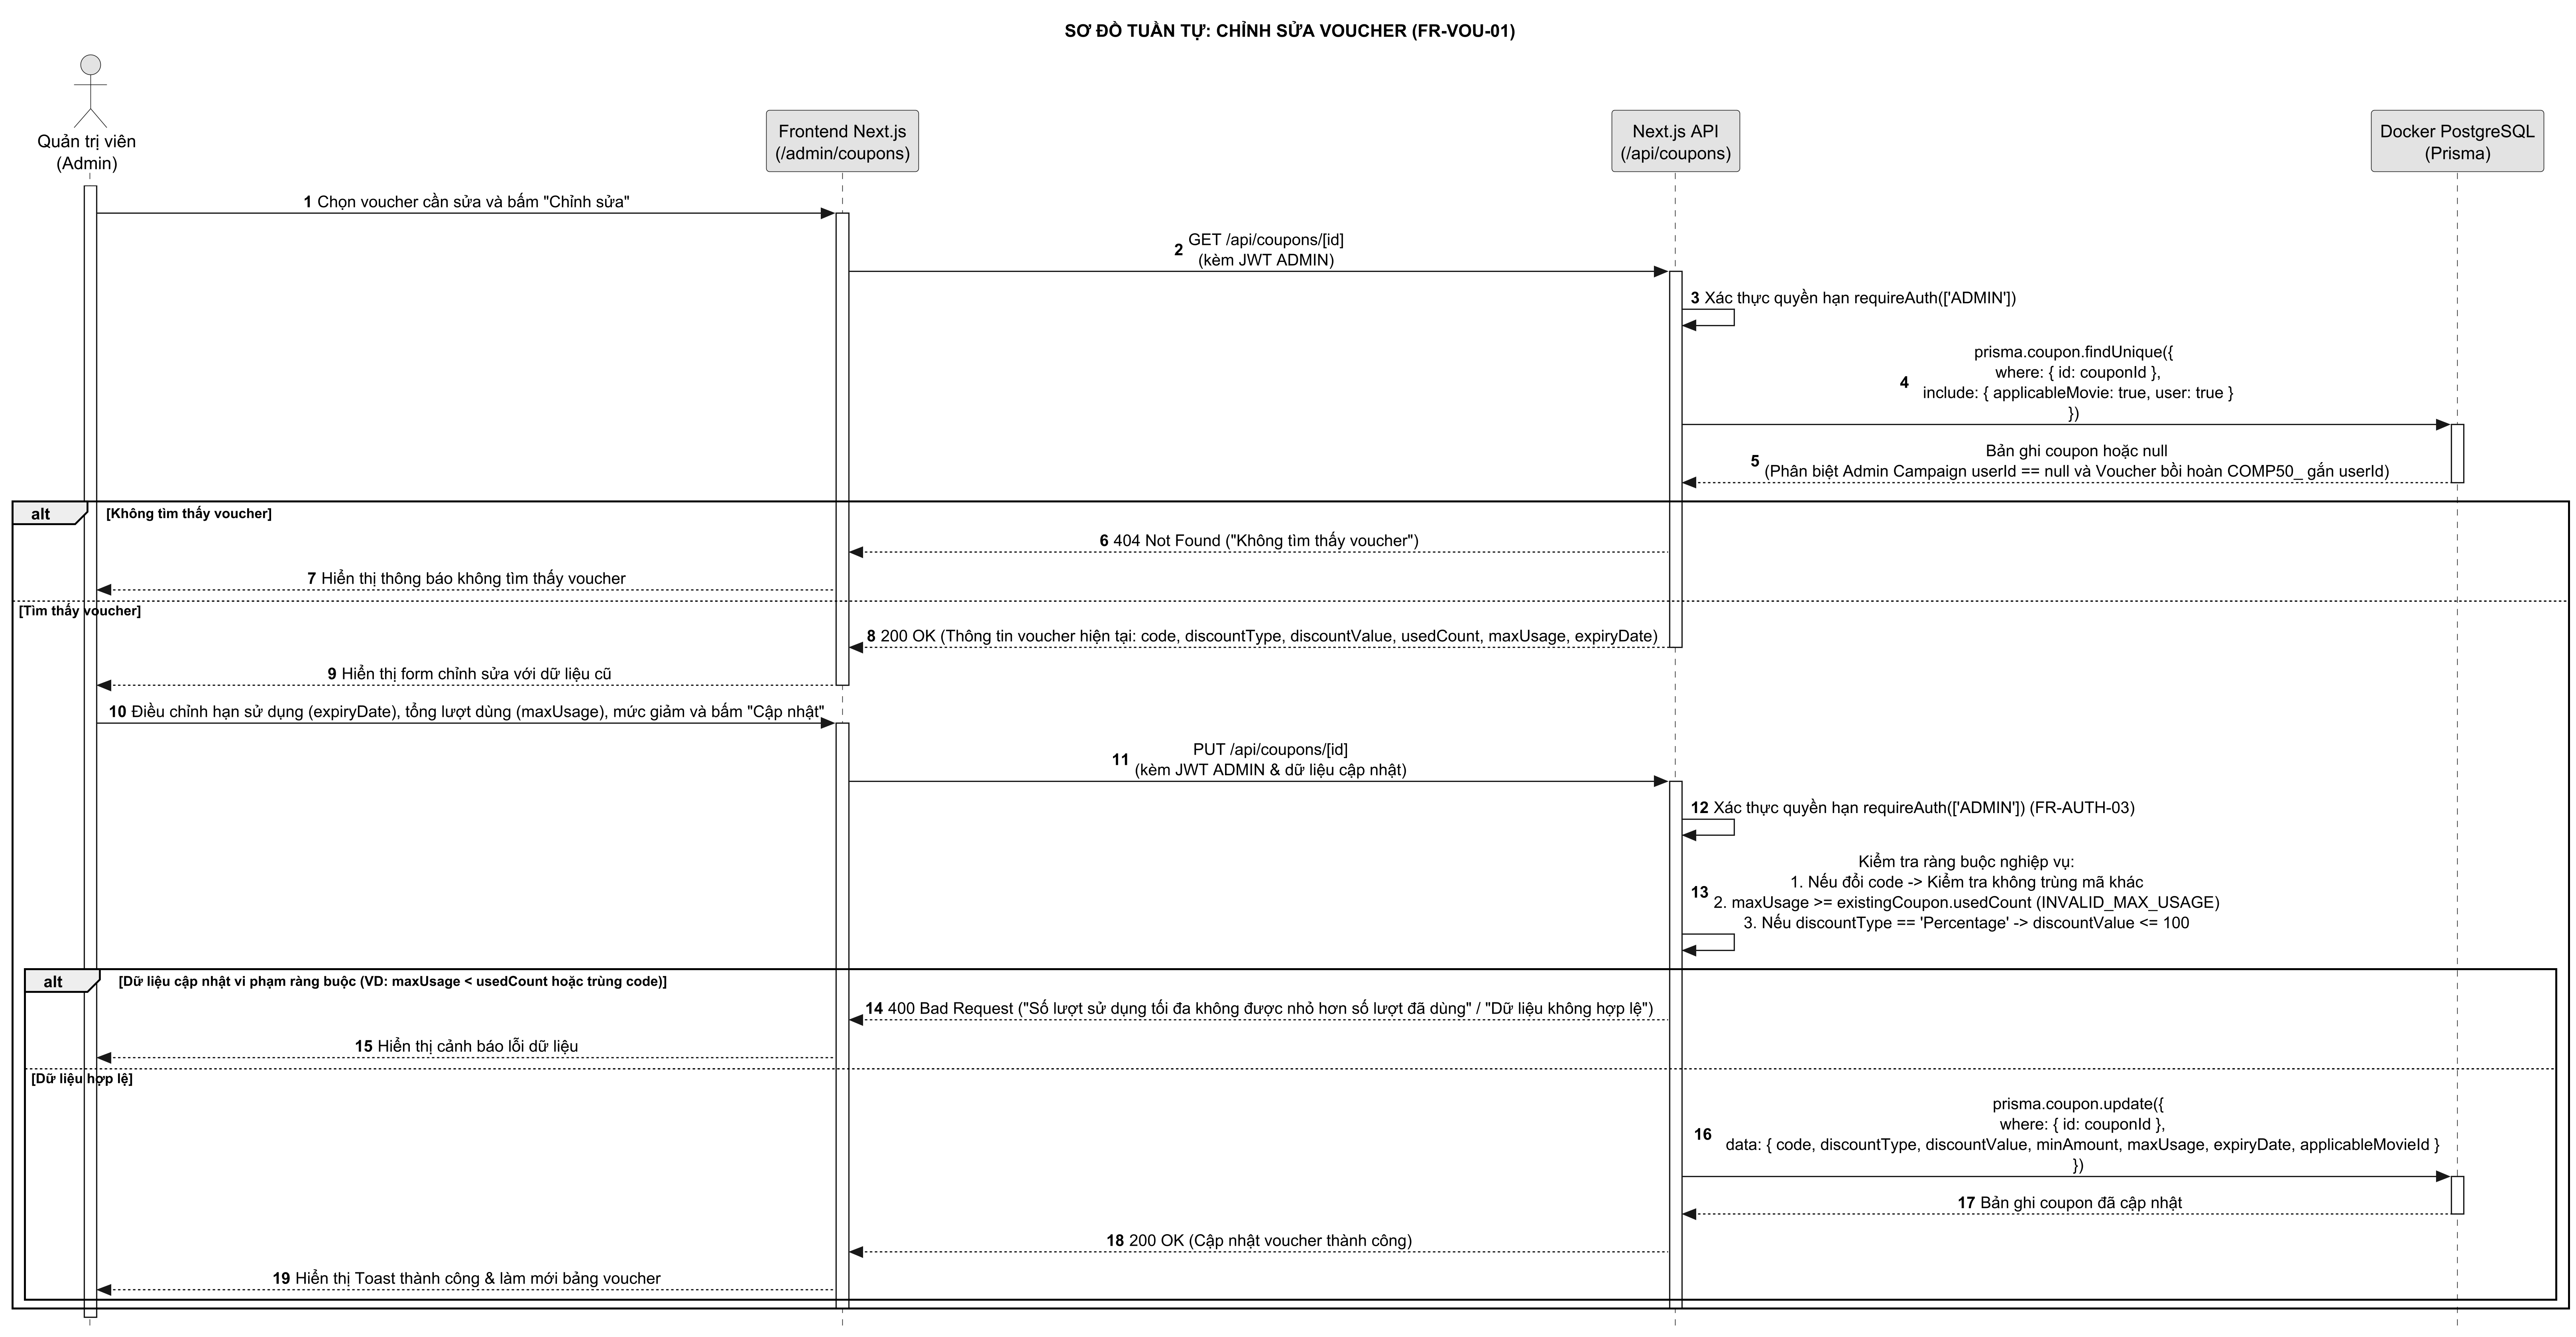
\includegraphics[width=\textwidth,height=0.80\textheight,keepaspectratio]{images/sequence/32_sua_voucher.png}
  \caption{Sequence Diagram: SƠ ĐỒ TUẦN TỰ: CHỈNH SỬA VOUCHER (FR-VOU-01)}
  \label{fig:seq_32}
\end{figure}

\subsection{SƠ ĐỒ TUẦN TỰ: XÓA / VÔ HIỆU HÓA VOUCHER (FR-VOU-01)}
\begin{figure}[H]
  \centering
  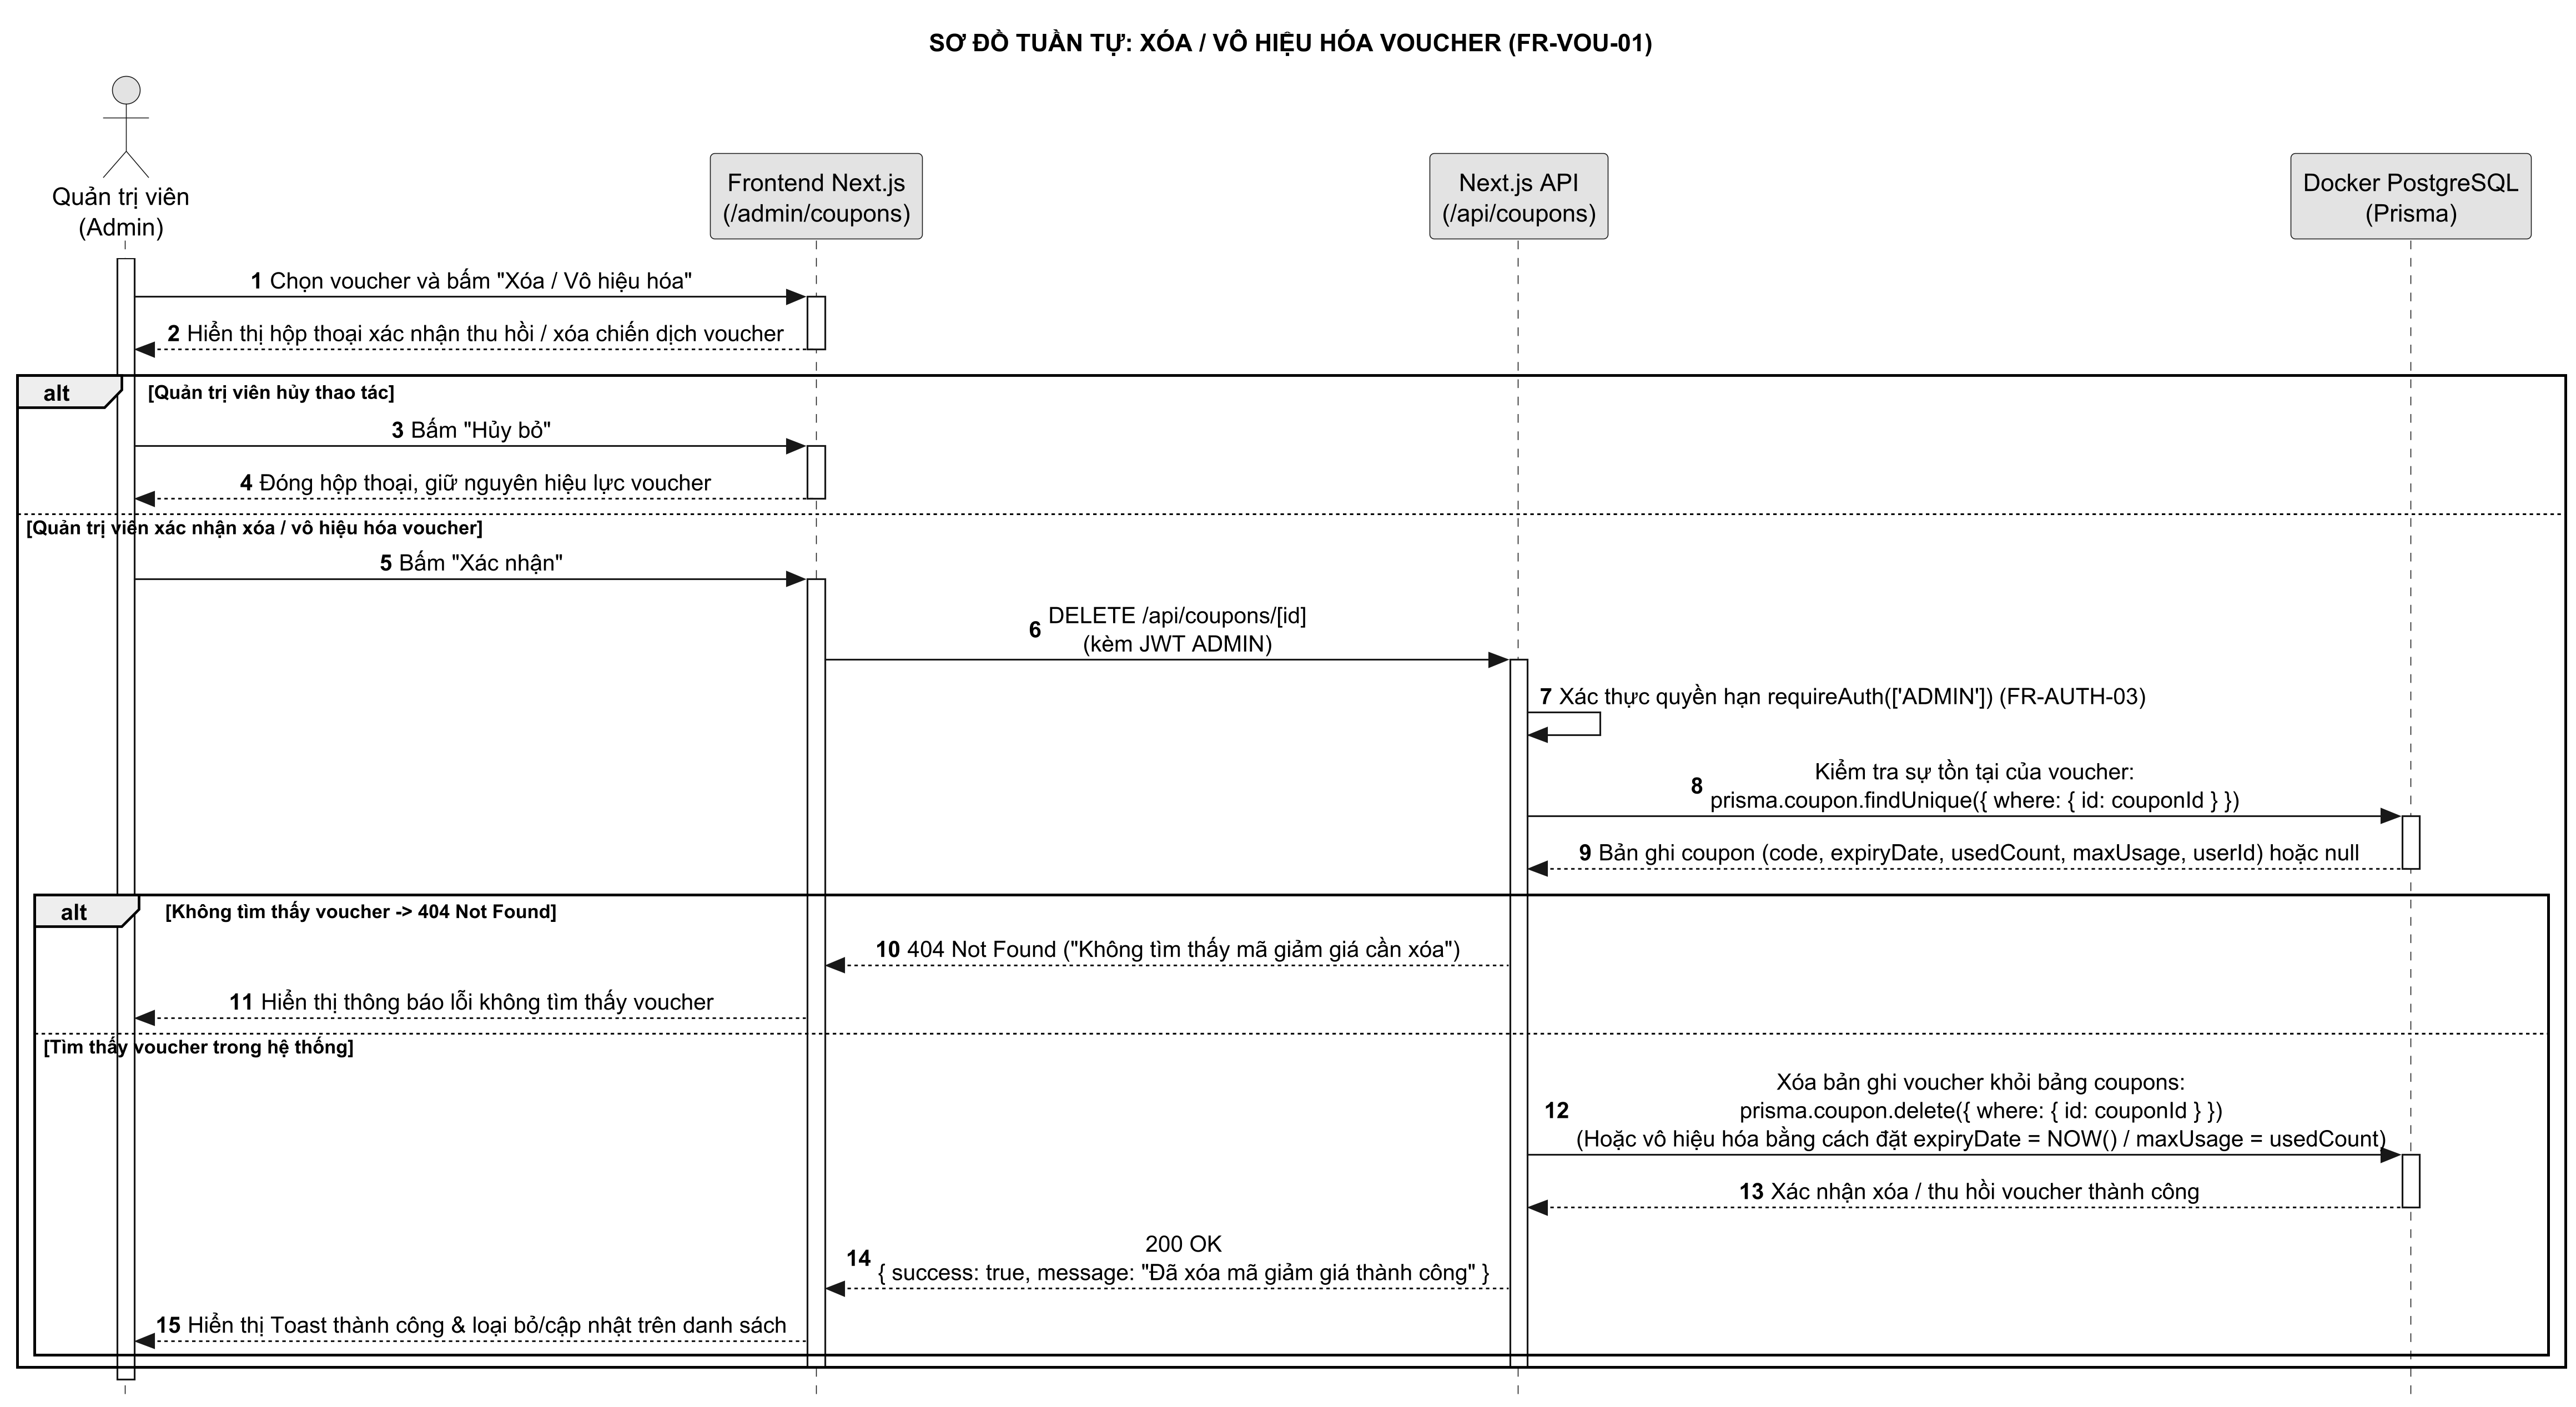
\includegraphics[width=\textwidth,height=0.80\textheight,keepaspectratio]{images/sequence/33_ngung_su_dung_voucher.png}
  \caption{Sequence Diagram: SƠ ĐỒ TUẦN TỰ: XÓA / VÔ HIỆU HÓA VOUCHER (FR-VOU-01)}
  \label{fig:seq_33}
\end{figure}

\subsection{SƠ ĐỒ TUẦN TỰ: QUẢN TRỊ LỊCH CHIẾU VÀ SUẤT CHIẾU (TỔNG QUAN - FR-ADM-03, FR-ADM-04, BR-01, BR-04, BR-08)}
\begin{figure}[H]
  \centering
  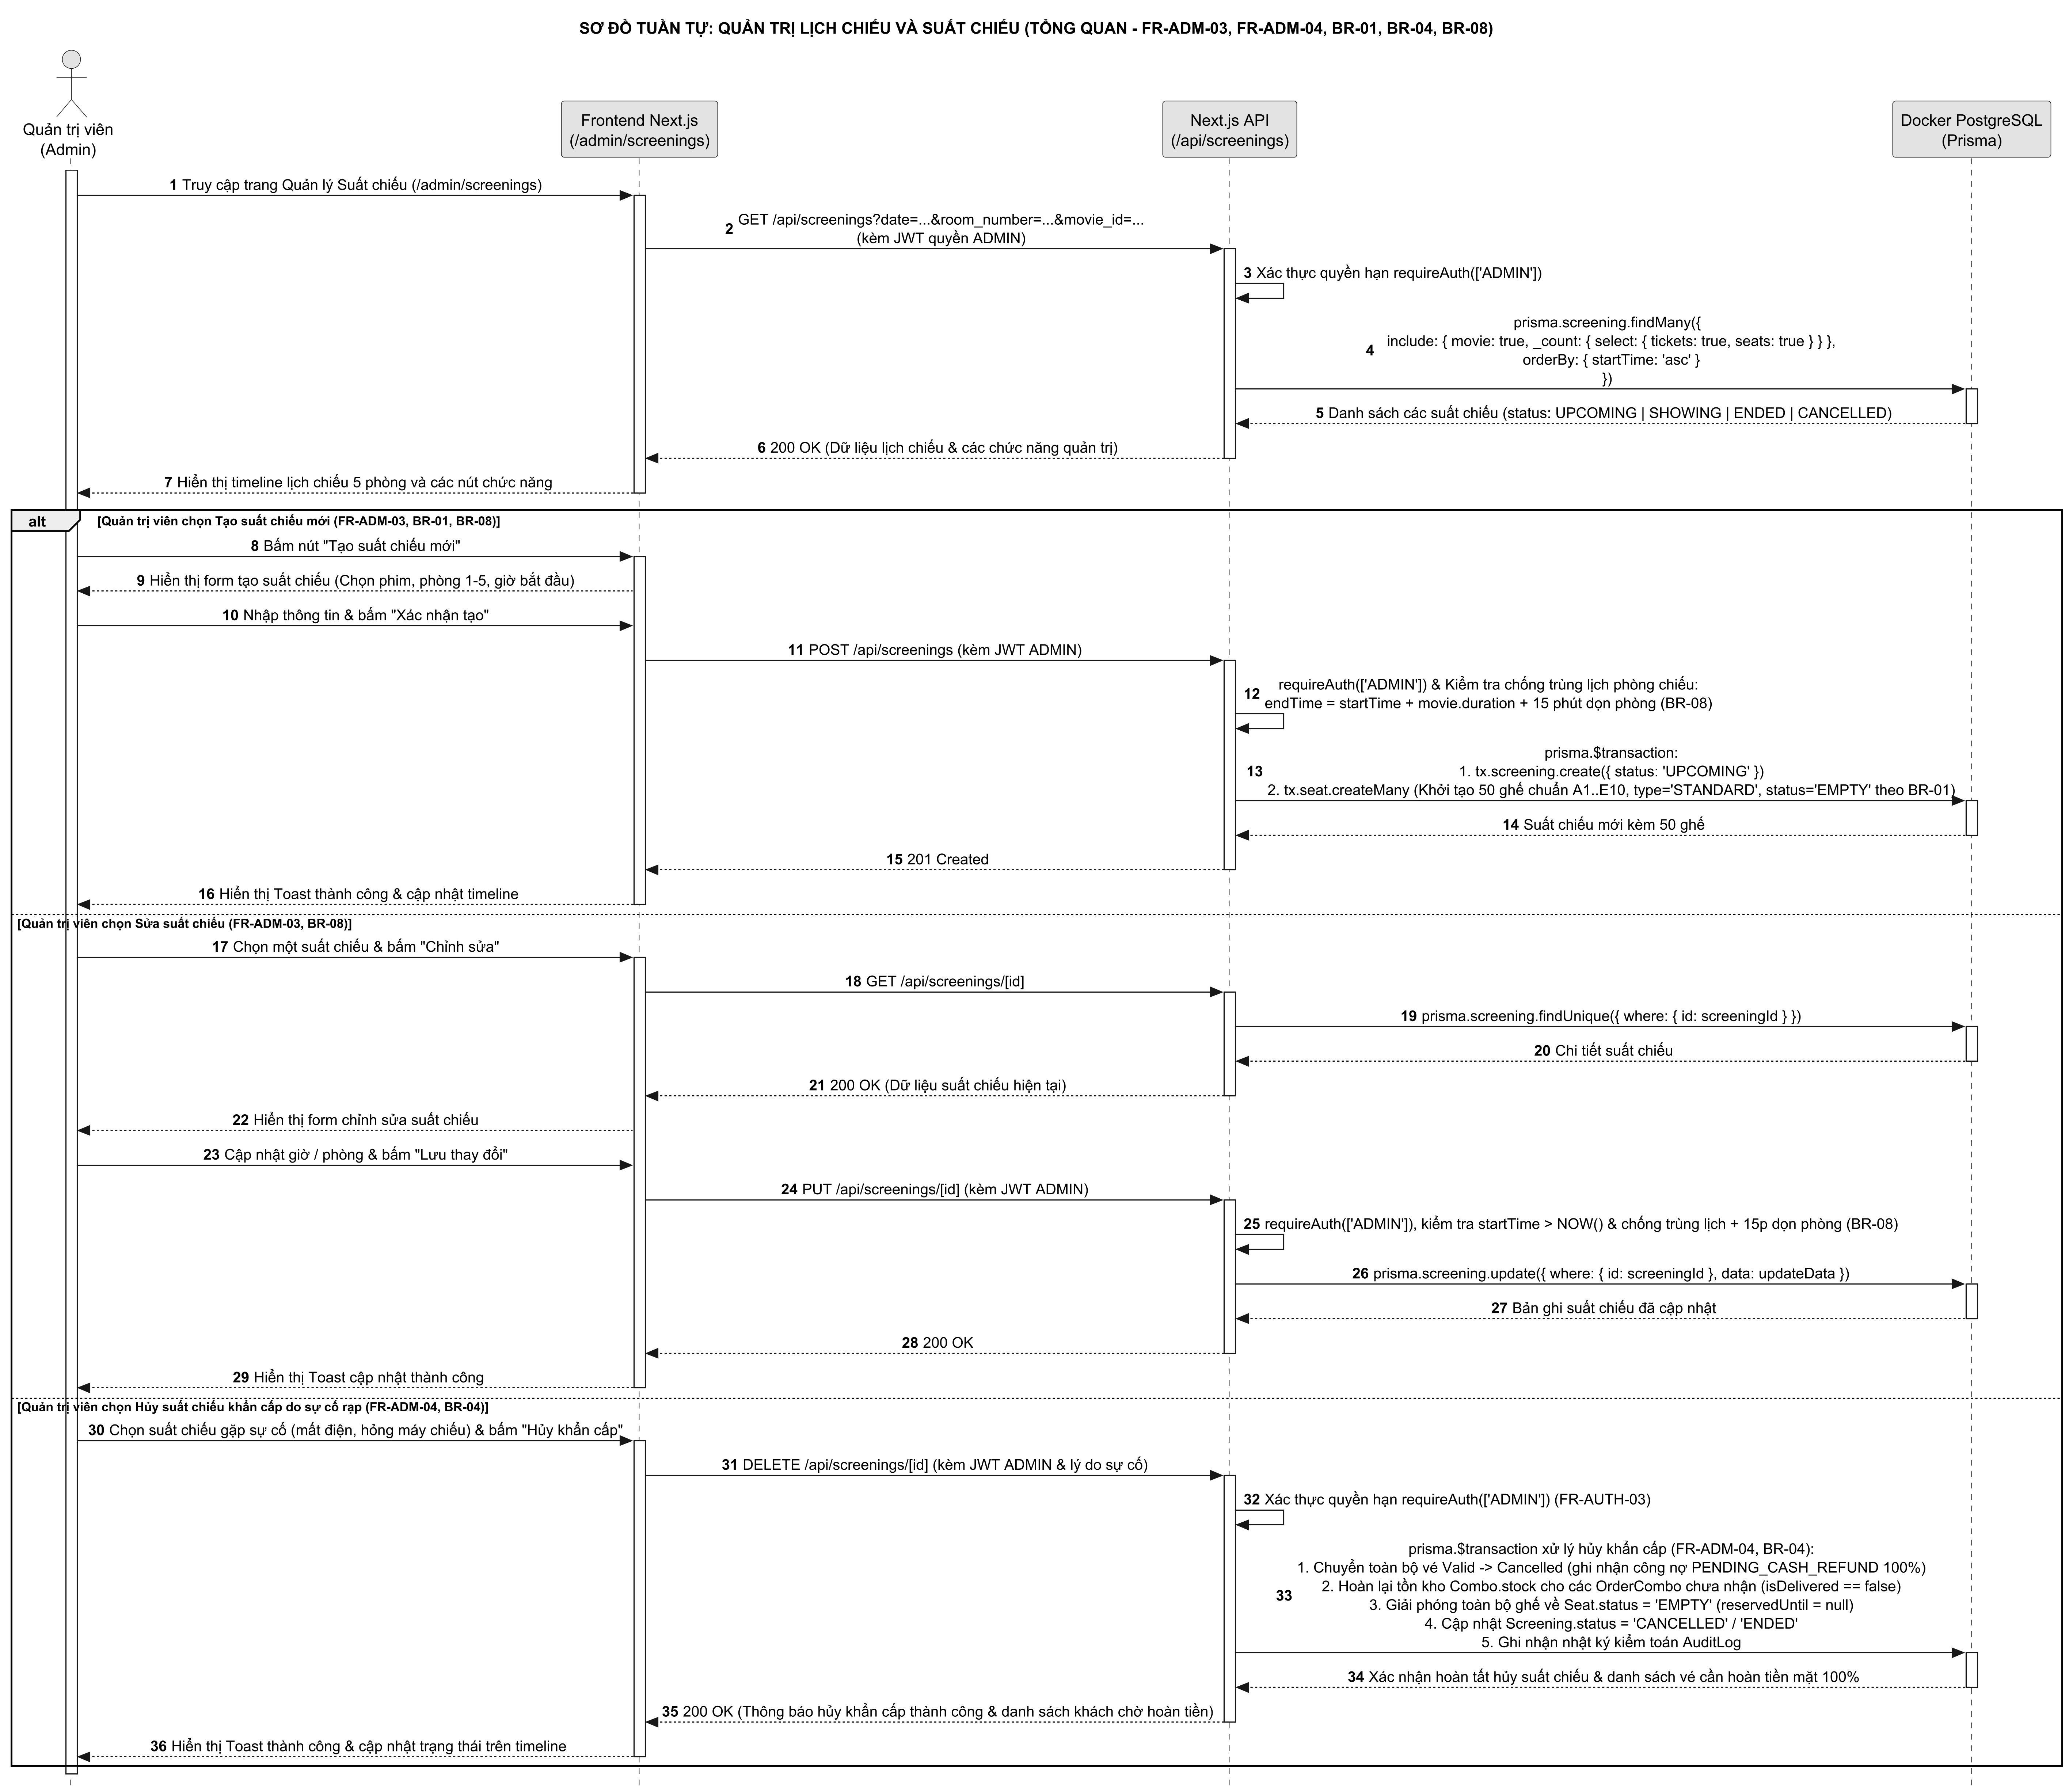
\includegraphics[width=\textwidth,height=0.80\textheight,keepaspectratio]{images/sequence/34_quan_ly_suat_chieu_tong_quan.png}
  \caption{Sequence Diagram: SƠ ĐỒ TUẦN TỰ: QUẢN TRỊ LỊCH CHIẾU VÀ SUẤT CHIẾU (TỔNG QUAN - FR-ADM-03, FR-ADM-04, BR-01, BR-04, BR-08)}
  \label{fig:seq_34}
\end{figure}

\subsection{SƠ ĐỒ TUẦN TỰ: THÊM MỚI SUẤT CHIẾU (FR-ADM-03, BR-01, BR-08)}
\begin{figure}[H]
  \centering
  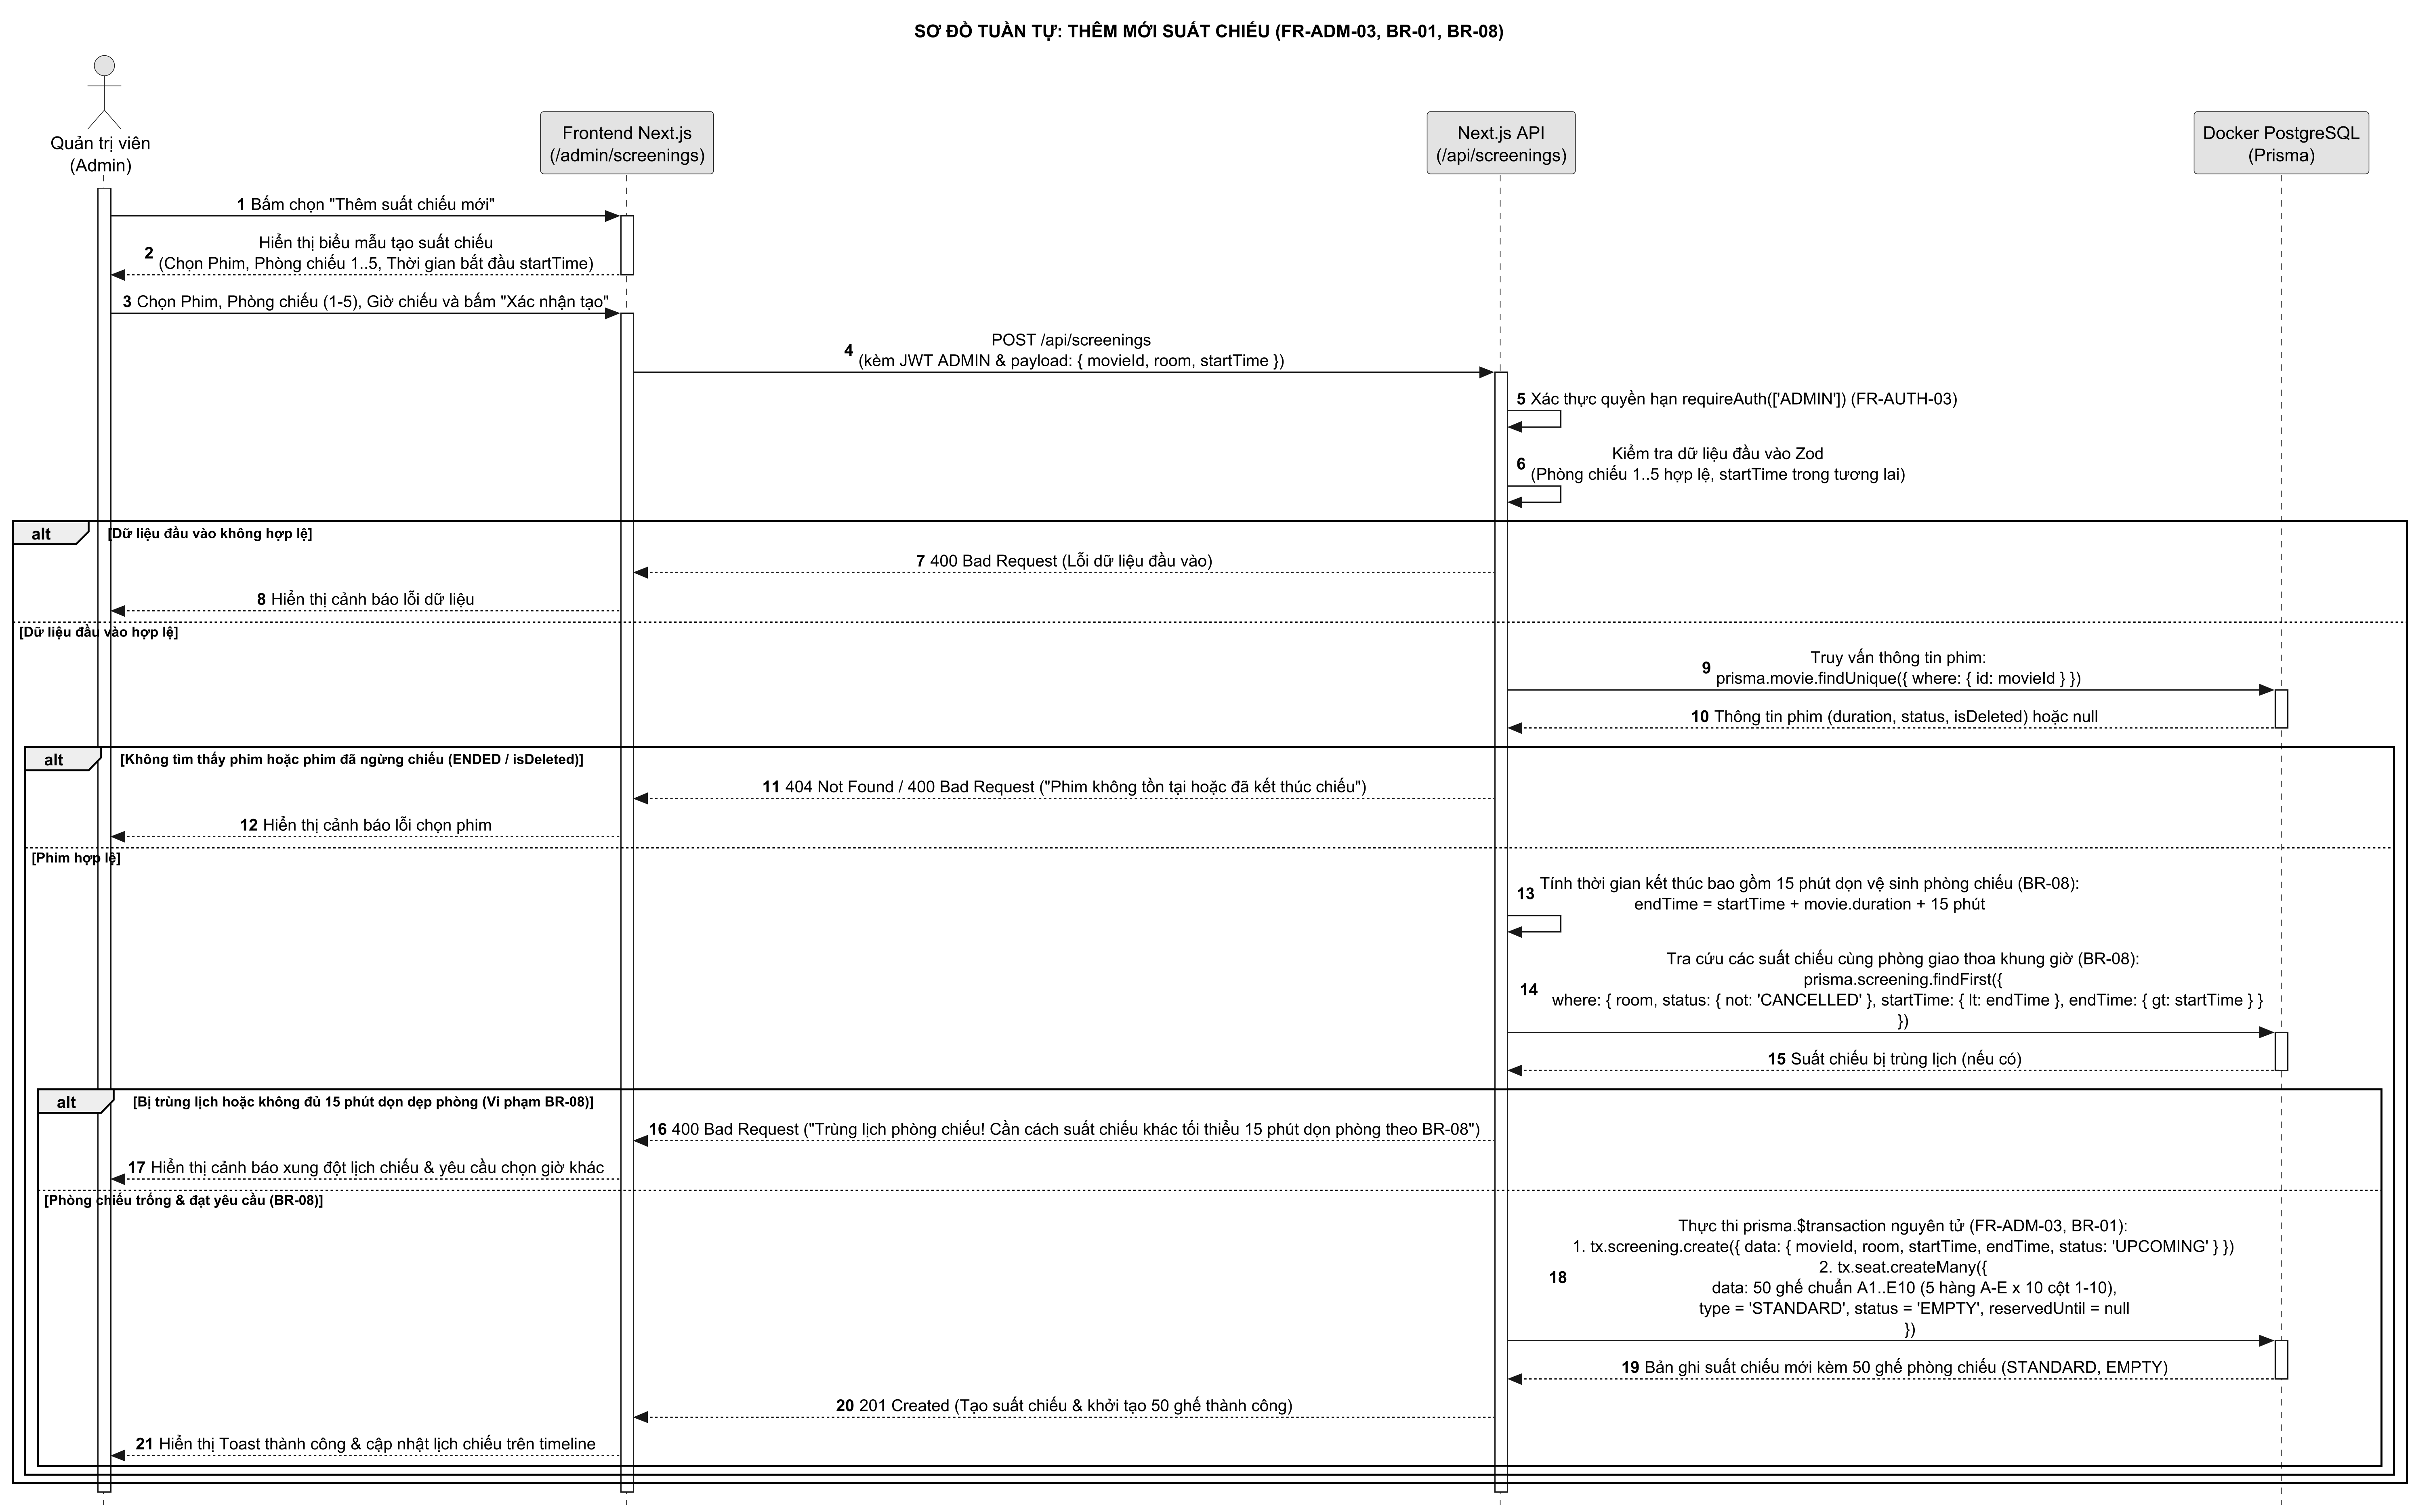
\includegraphics[width=\textwidth,height=0.80\textheight,keepaspectratio]{images/sequence/35_them_suat_chieu.png}
  \caption{Sequence Diagram: SƠ ĐỒ TUẦN TỰ: THÊM MỚI SUẤT CHIẾU (FR-ADM-03, BR-01, BR-08)}
  \label{fig:seq_35}
\end{figure}

\subsection{SƠ ĐỒ TUẦN TỰ: KIỂM TRA CHỐNG TRÙNG LỊCH PHÒNG CHIẾU \& ĐỘ PHÙ HỢP SUẤT CHIẾU (BR-02, BR-08)}
\begin{figure}[H]
  \centering
  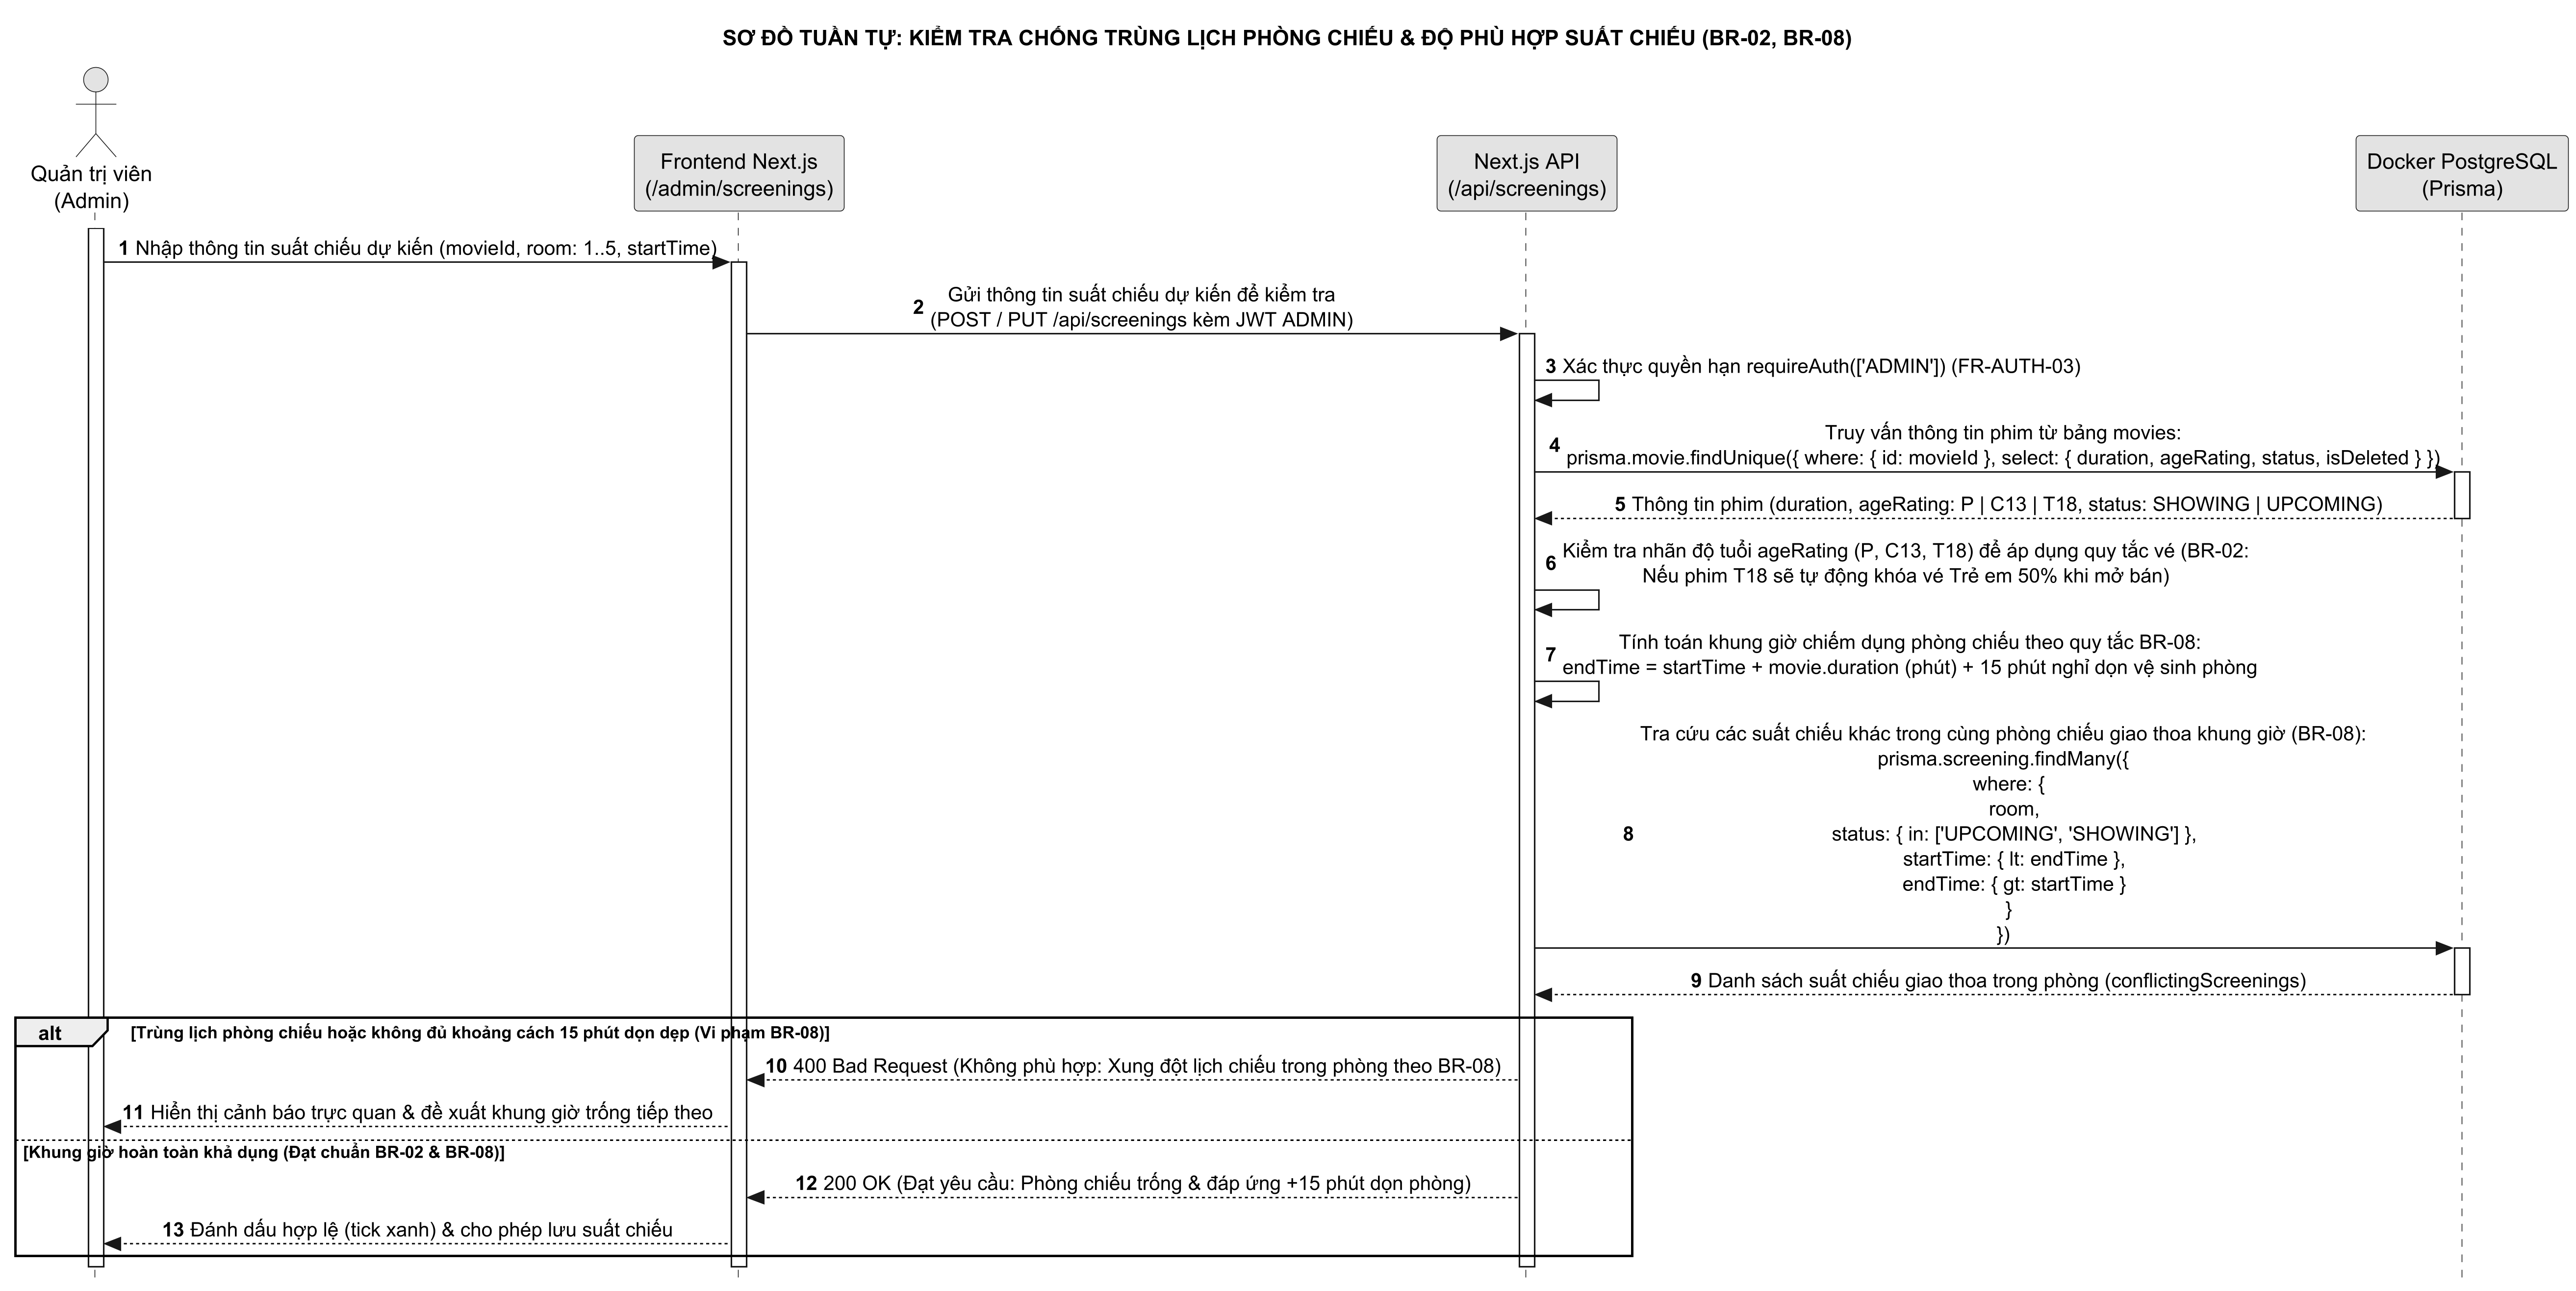
\includegraphics[width=\textwidth,height=0.80\textheight,keepaspectratio]{images/sequence/36_kiem_tra_do_phu_hop_suat_chieu.png}
  \caption{Sequence Diagram: SƠ ĐỒ TUẦN TỰ: KIỂM TRA CHỐNG TRÙNG LỊCH PHÒNG CHIẾU \& ĐỘ PHÙ HỢP SUẤT CHIẾU (BR-02, BR-08)}
  \label{fig:seq_36}
\end{figure}

\subsection{SƠ ĐỒ TUẦN TỰ: CHỈNH SỬA SUẤT CHIẾU (FR-ADM-03, BR-08)}
\begin{figure}[H]
  \centering
  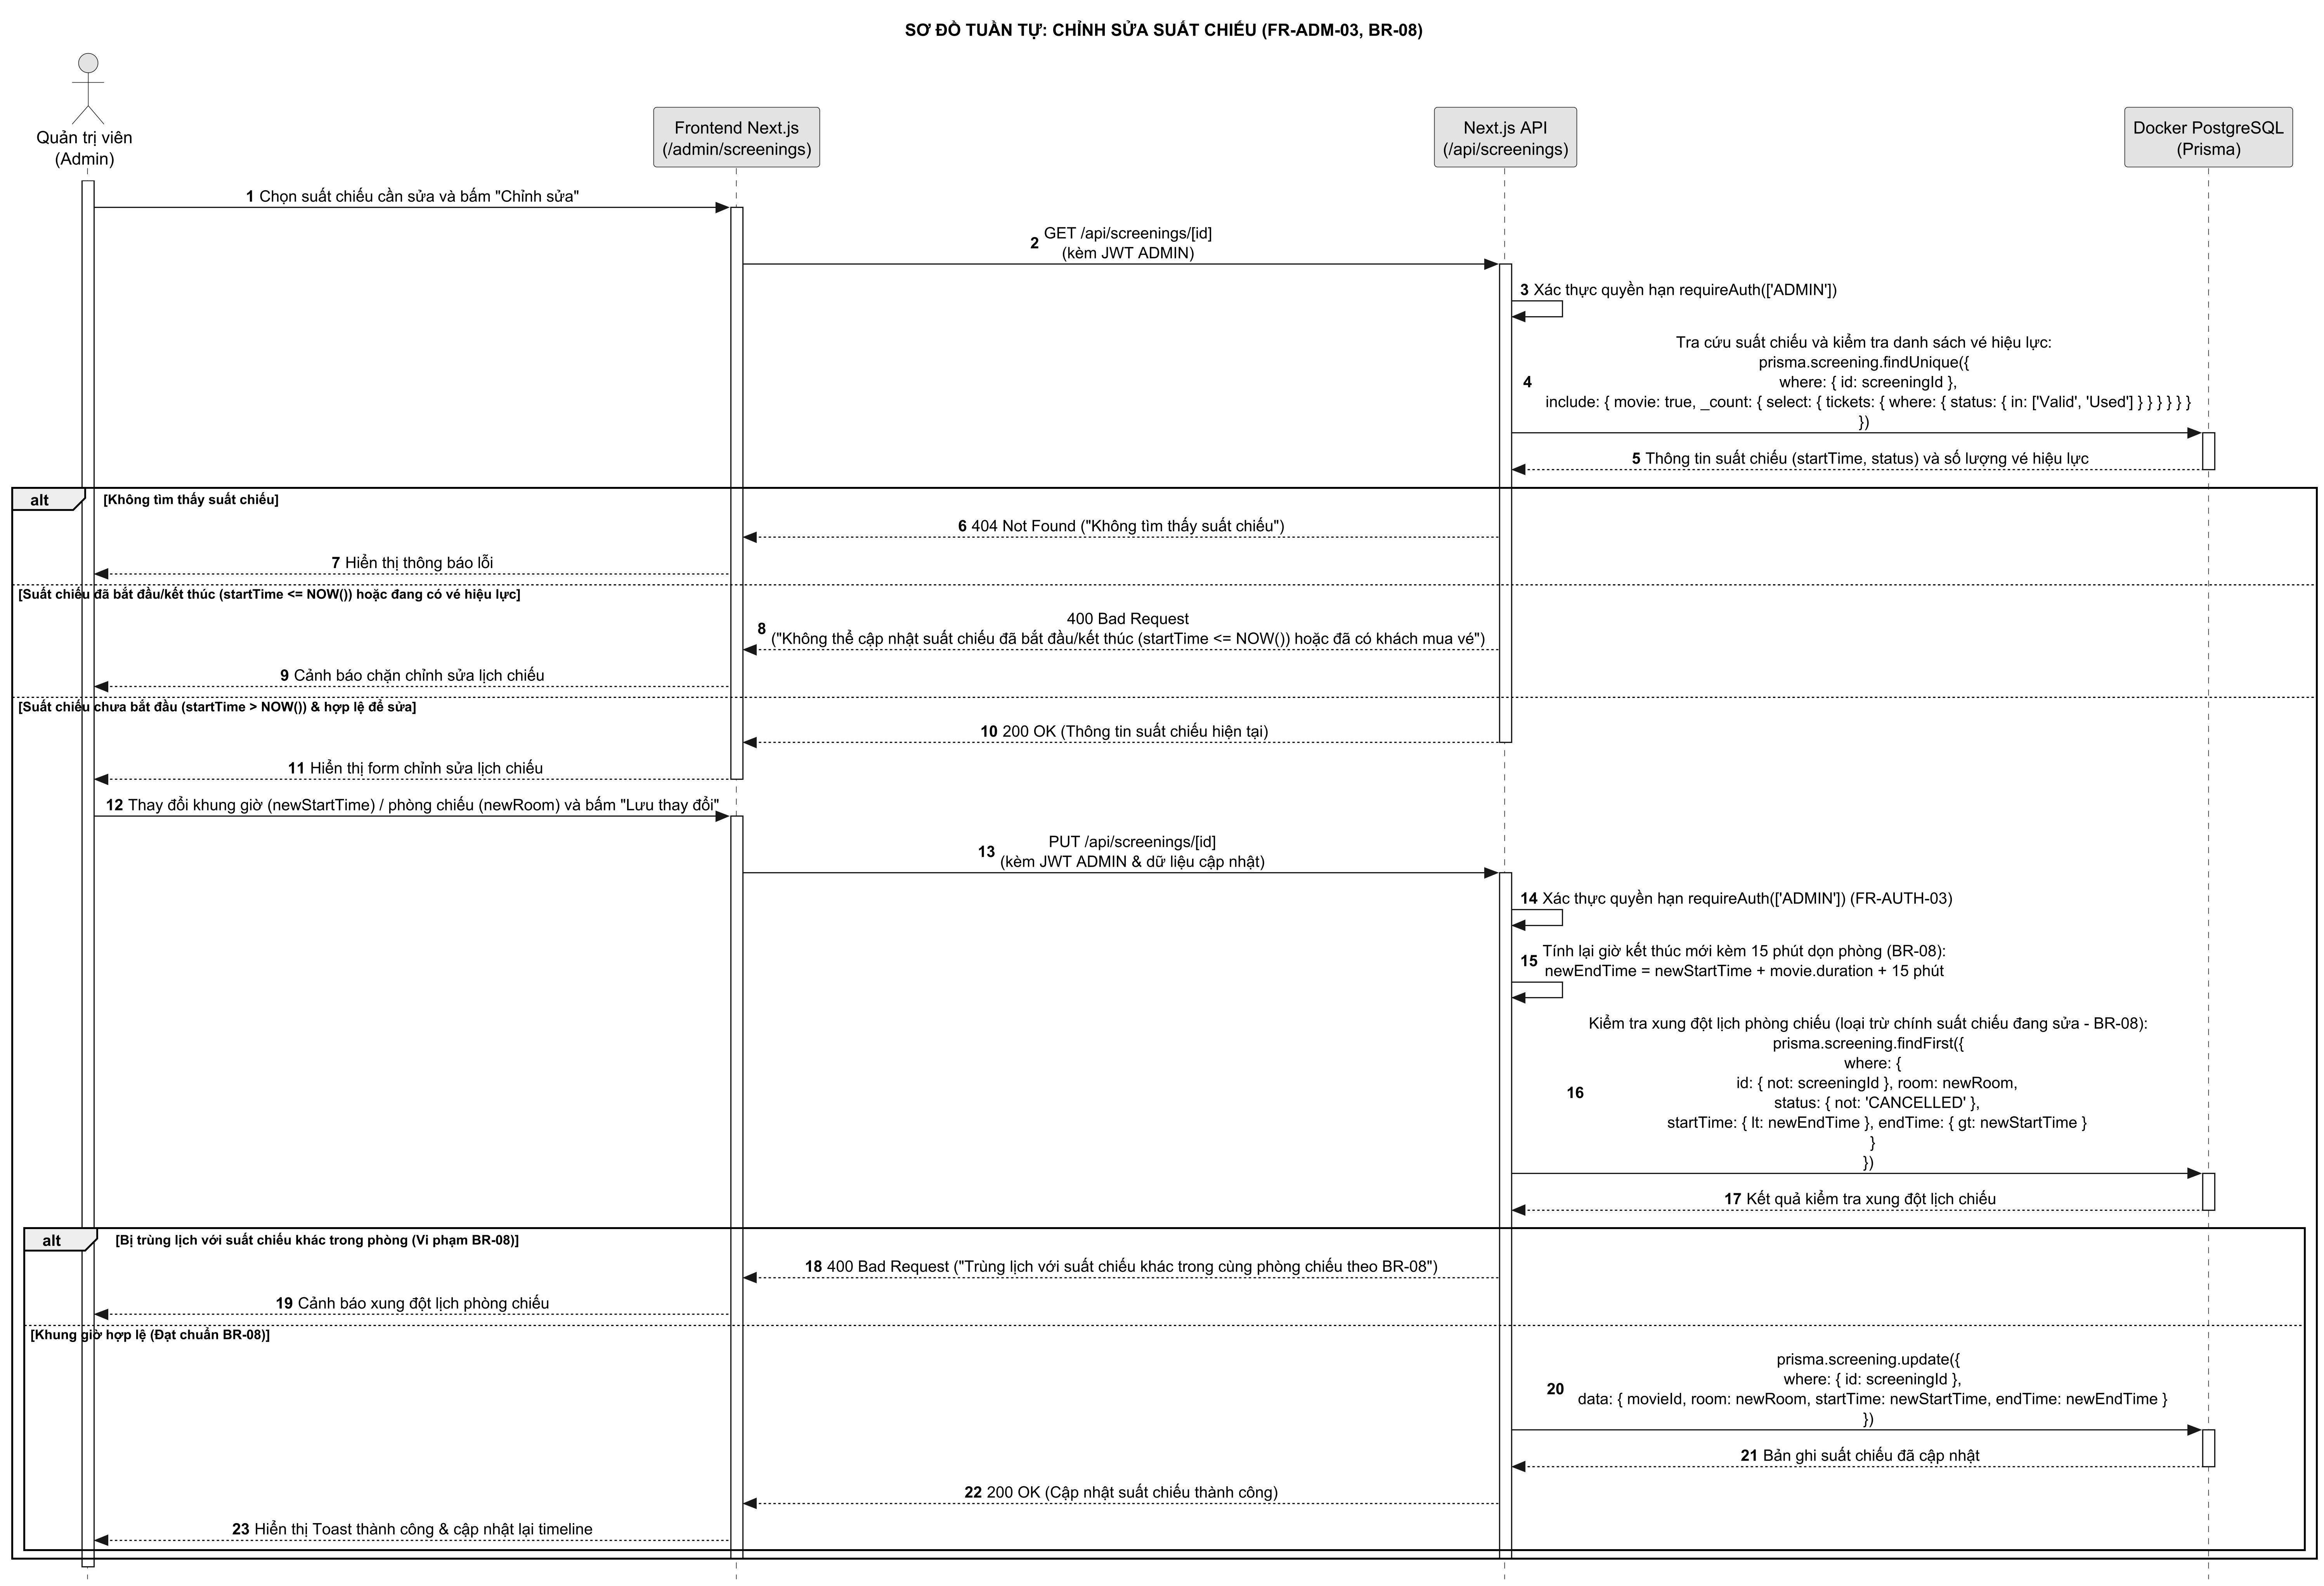
\includegraphics[width=\textwidth,height=0.80\textheight,keepaspectratio]{images/sequence/37_sua_suat_chieu.png}
  \caption{Sequence Diagram: SƠ ĐỒ TUẦN TỰ: CHỈNH SỬA SUẤT CHIẾU (FR-ADM-03, BR-08)}
  \label{fig:seq_37}
\end{figure}

\subsection{SƠ ĐỒ TUẦN TỰ: BÁO CÁO DOANH THU \& DASHBOARD TÀI CHÍNH (ADMIN DASHBOARD \& REPORTS)}
\begin{figure}[H]
  \centering
  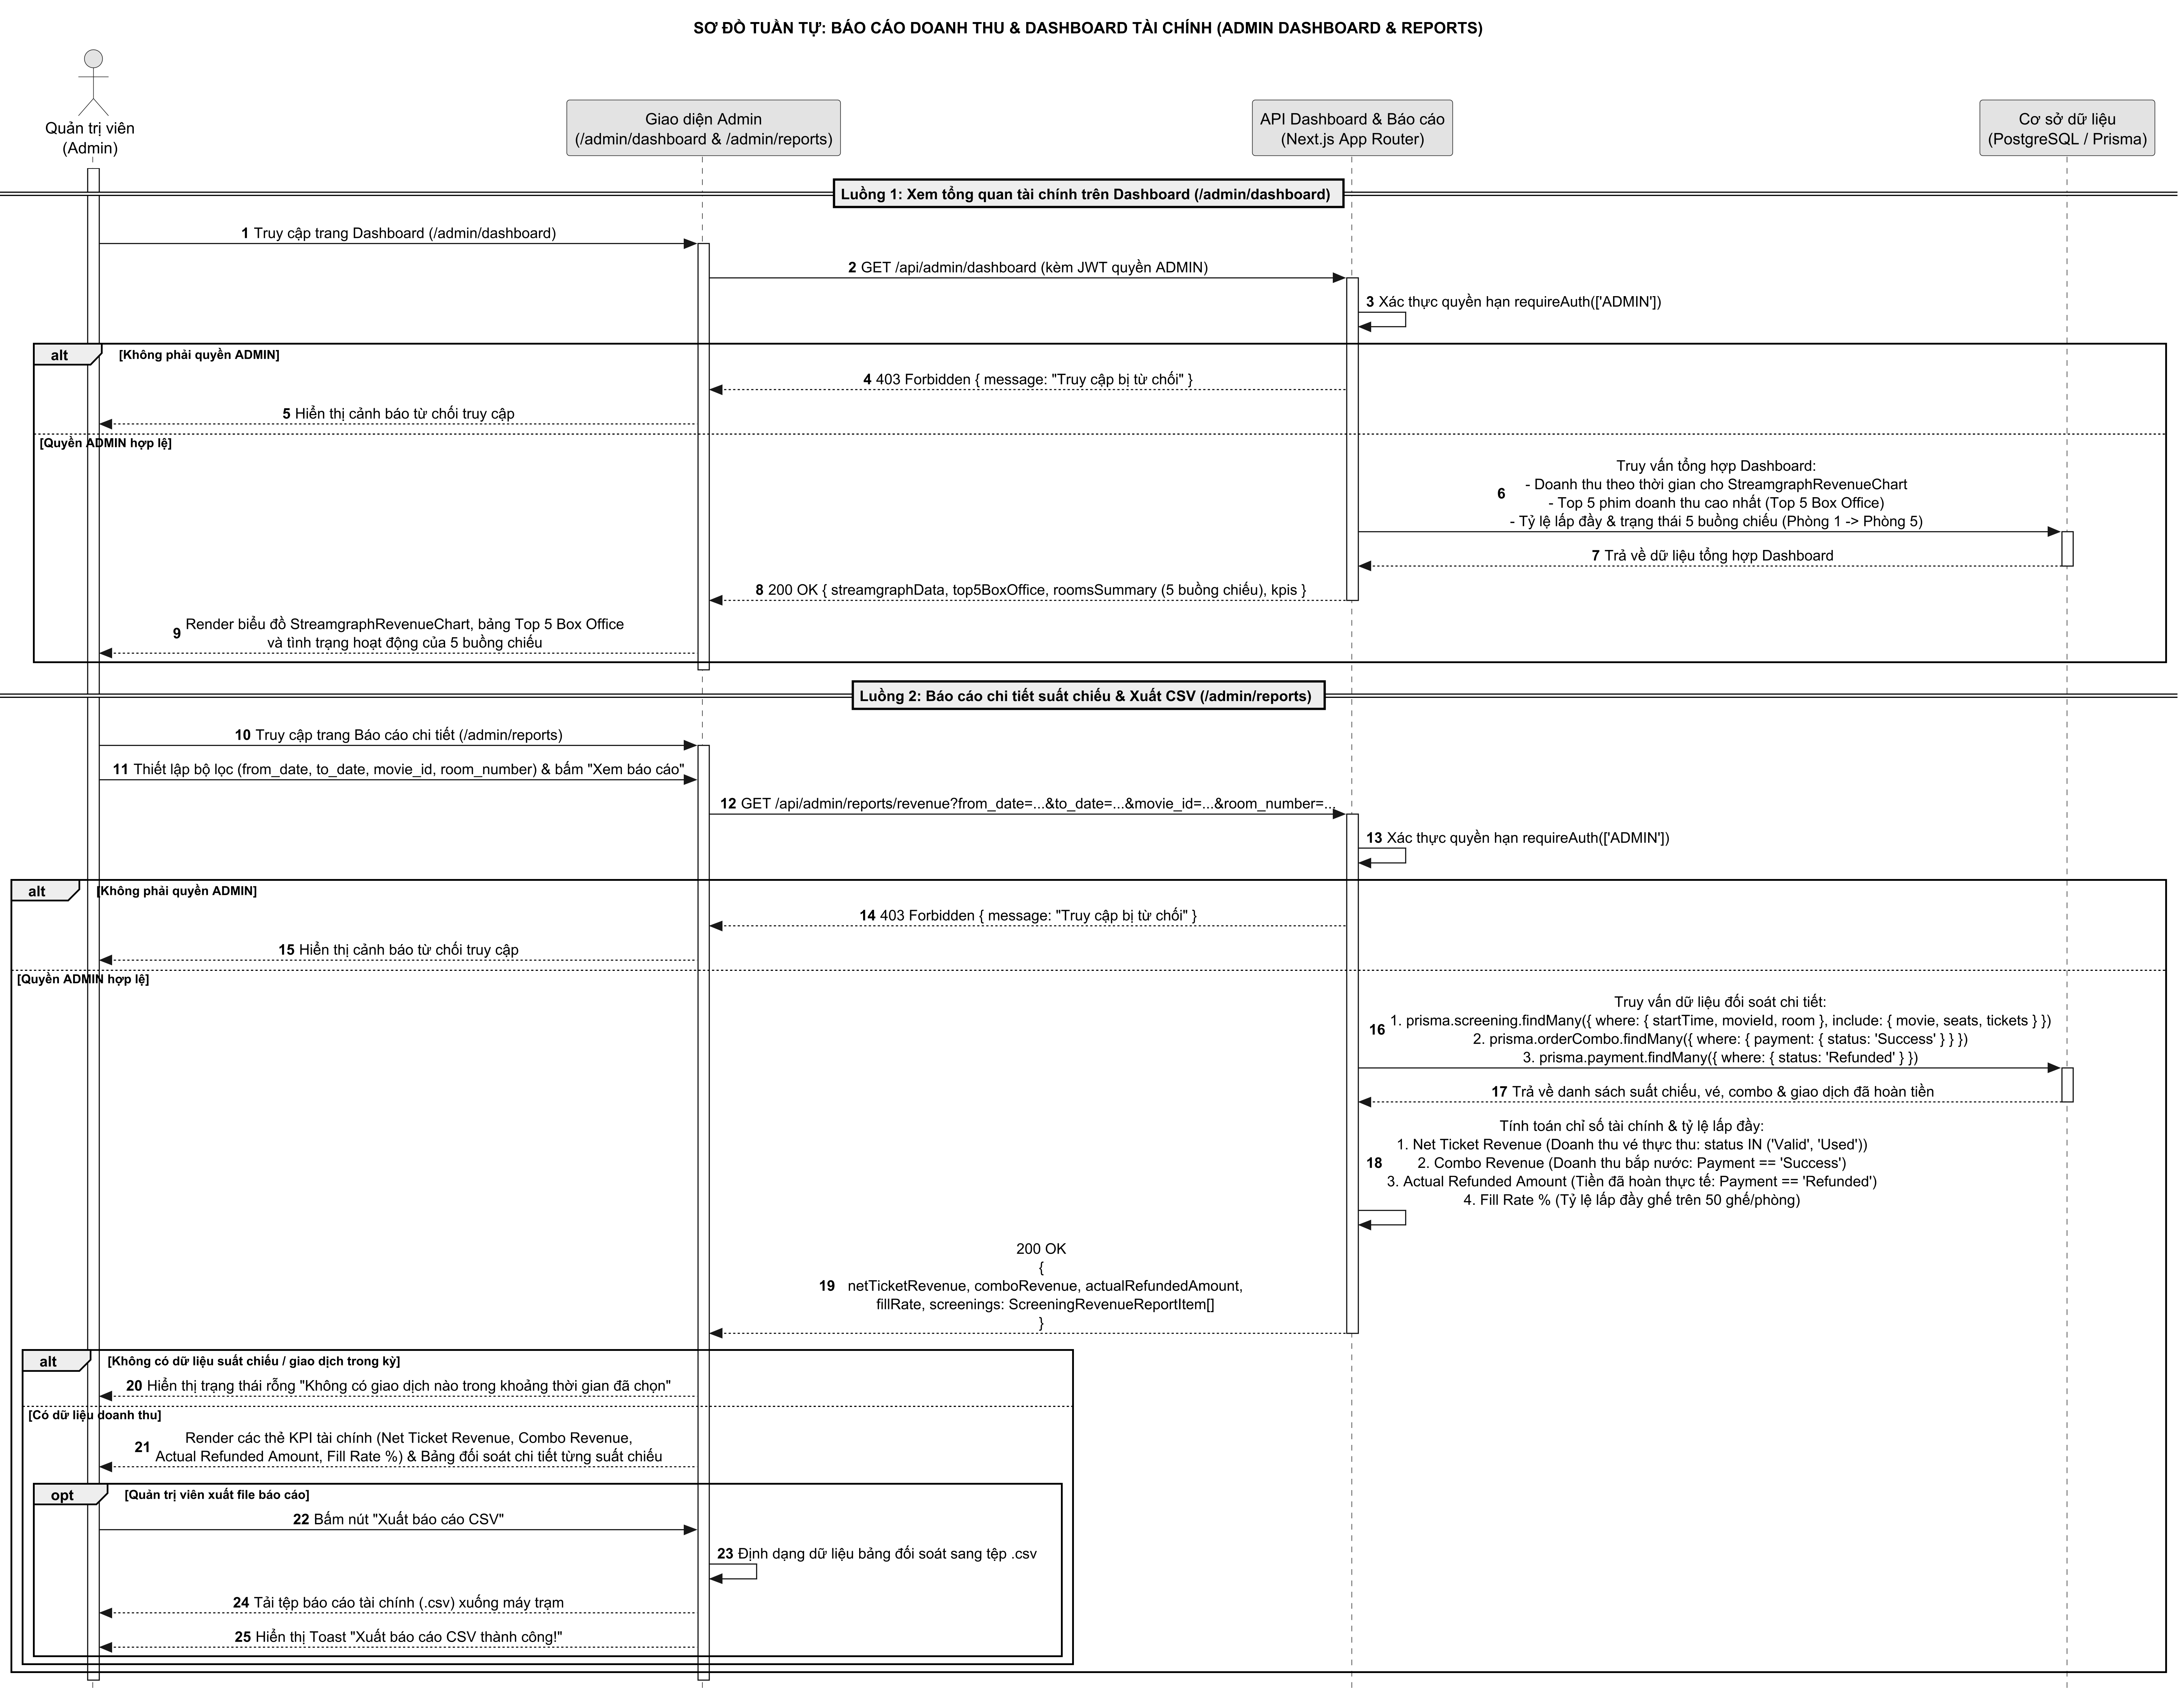
\includegraphics[width=\textwidth,height=0.80\textheight,keepaspectratio]{images/sequence/38_bao_cao_doanh_thu_tai_chinh.png}
  \caption{Sequence Diagram: SƠ ĐỒ TUẦN TỰ: BÁO CÁO DOANH THU \& DASHBOARD TÀI CHÍNH (ADMIN DASHBOARD \& REPORTS)}
  \label{fig:seq_38}
\end{figure}


\section{Lược đồ Activity (Biểu đồ hoạt động)}
Hệ thống gồm 17 lược đồ hoạt động (Activity Diagram) mô tả luồng xử lý nghiệp vụ, các nhánh rẽ điều kiện và xử lý ngoại lệ cho toàn bộ các chức năng chính của LumiCinema.

\subsection{SƠ ĐỒ HOẠT ĐỘNG: ĐĂNG NHẬP \& PHÂN QUYỀN ĐIỀU HƯỚNG (LOGIN \& RBAC ROUTING)}
\begin{figure}[H]
  \centering
  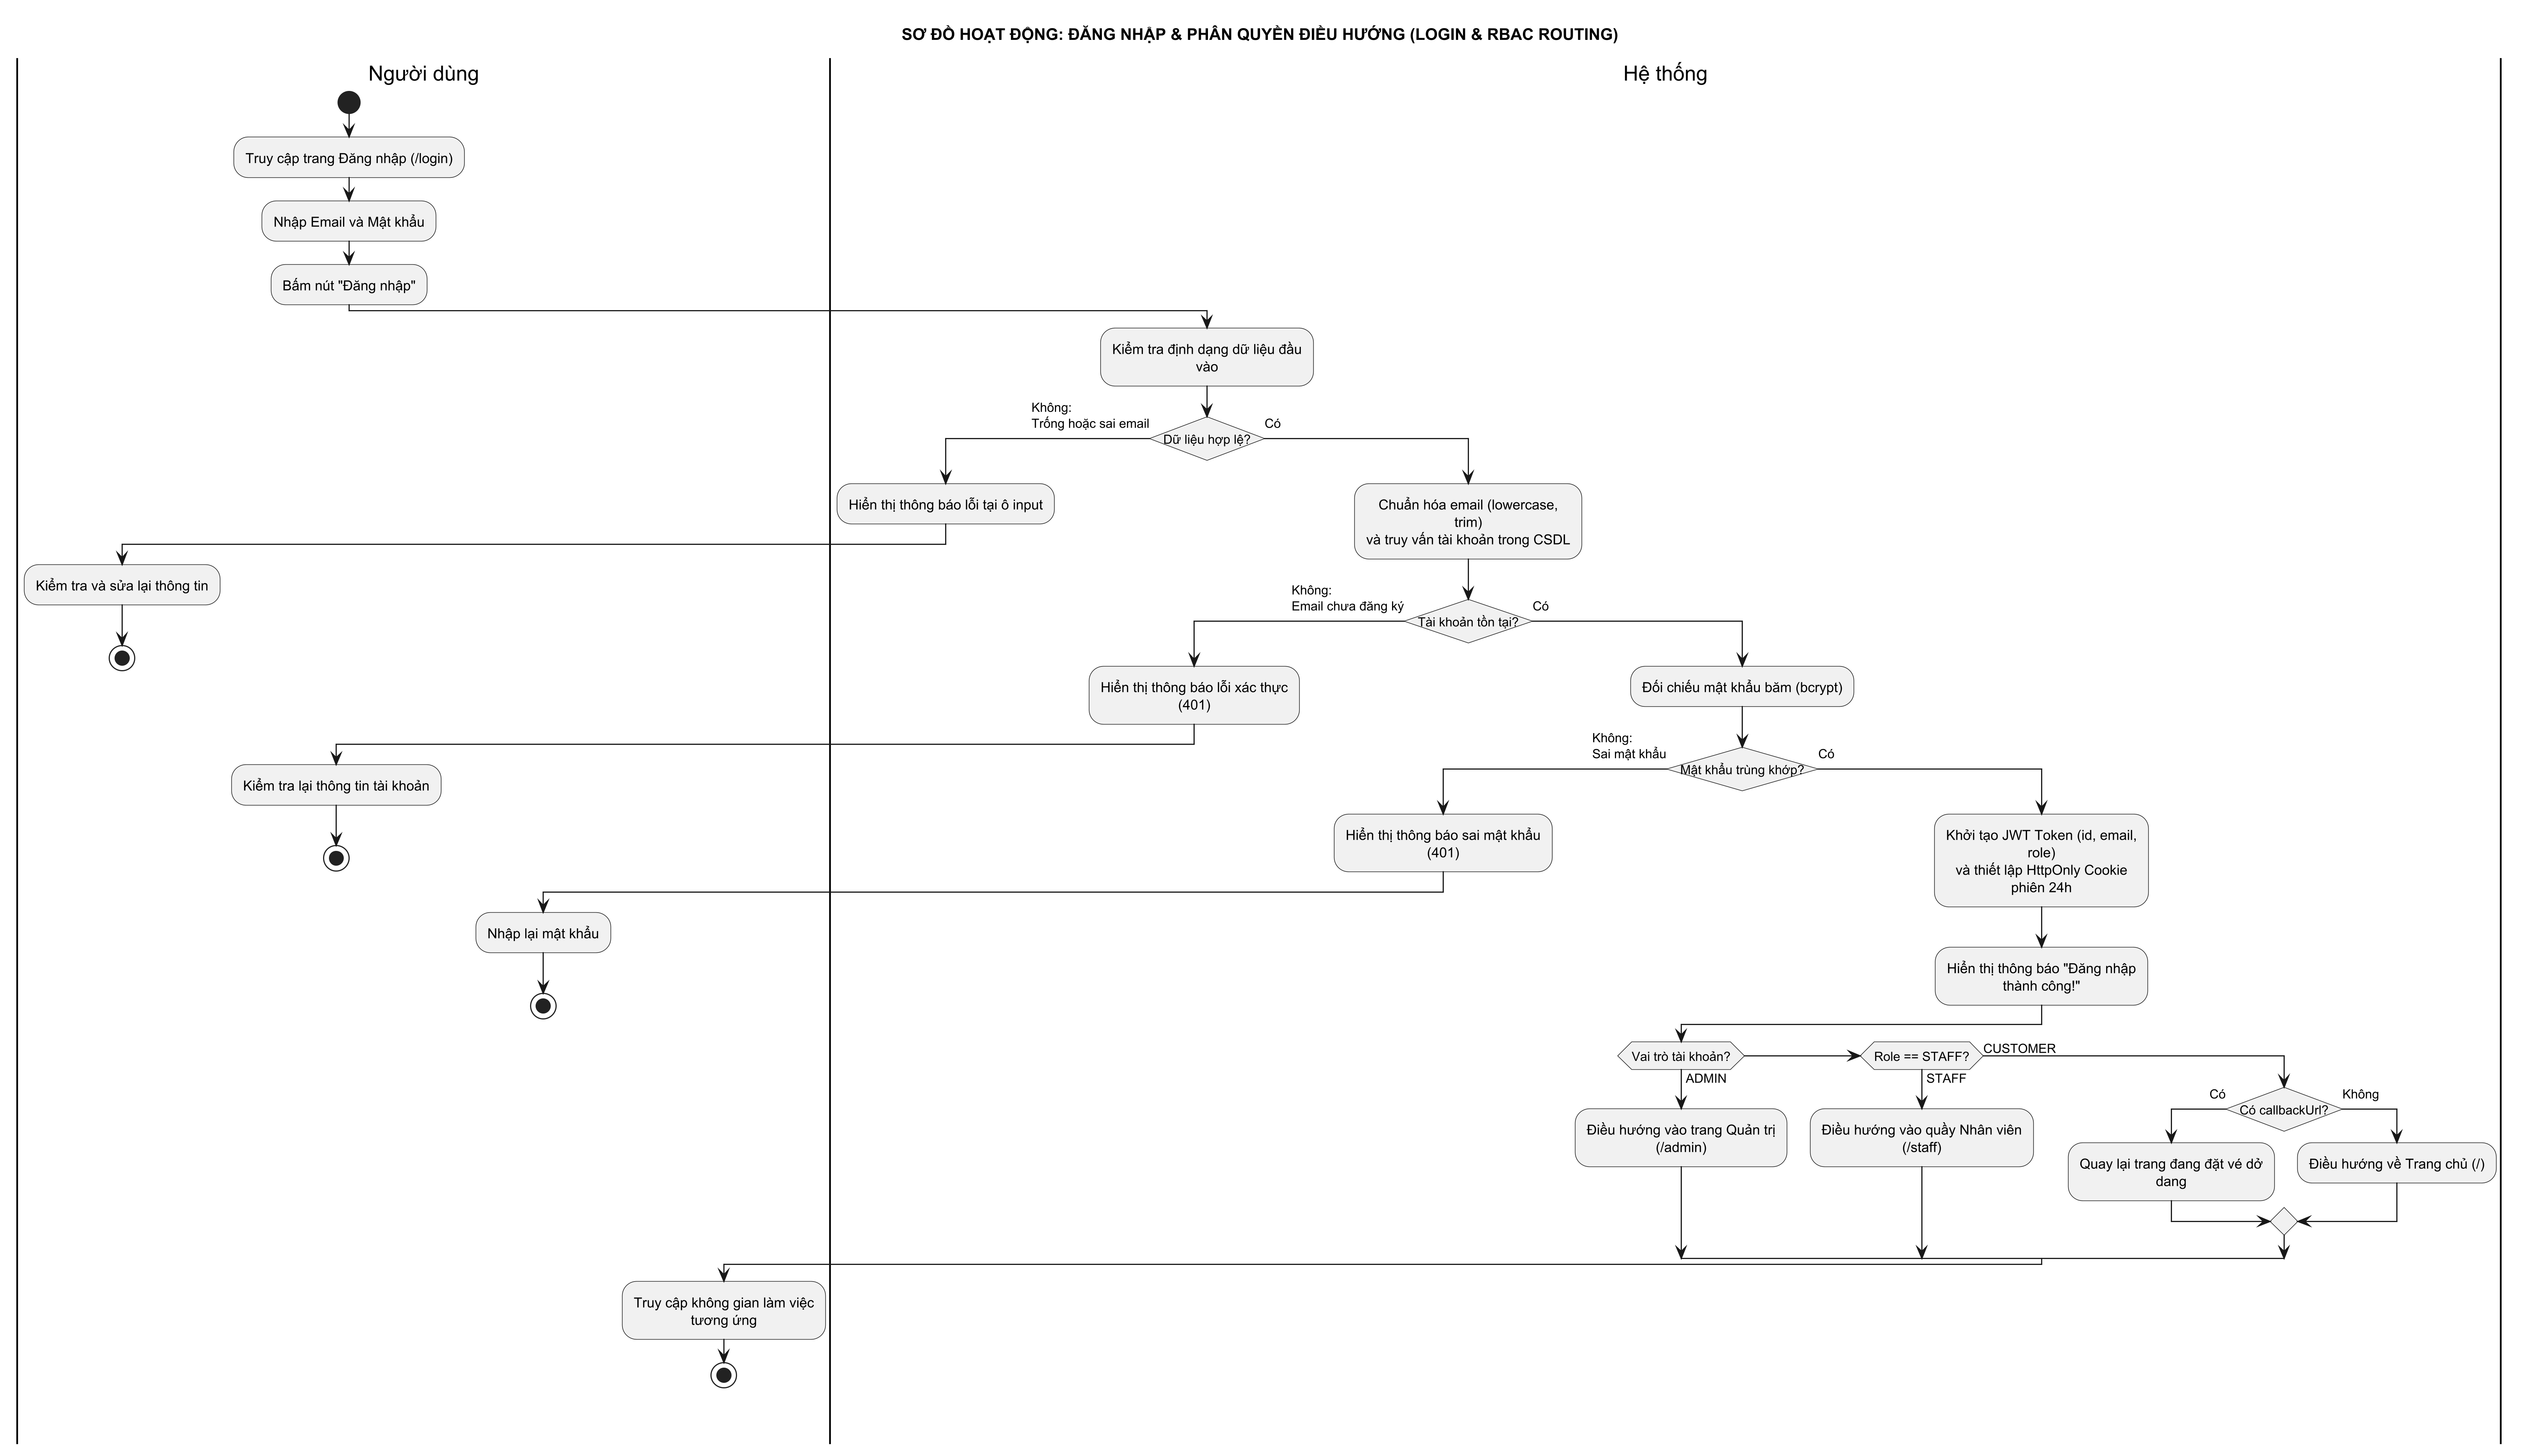
\includegraphics[width=\textwidth,height=0.80\textheight,keepaspectratio]{images/activity/01_dang_nhap.png}
  \caption{Activity Diagram: SƠ ĐỒ HOẠT ĐỘNG: ĐĂNG NHẬP \& PHÂN QUYỀN ĐIỀU HƯỚNG (LOGIN \& RBAC ROUTING)}
  \label{fig:act_01}
\end{figure}

\subsection{SƠ ĐỒ HOẠT ĐỘNG: ĐĂNG KÝ TÀI KHOẢN KHÁCH HÀNG (CUSTOMER SIGN UP)}
\begin{figure}[H]
  \centering
  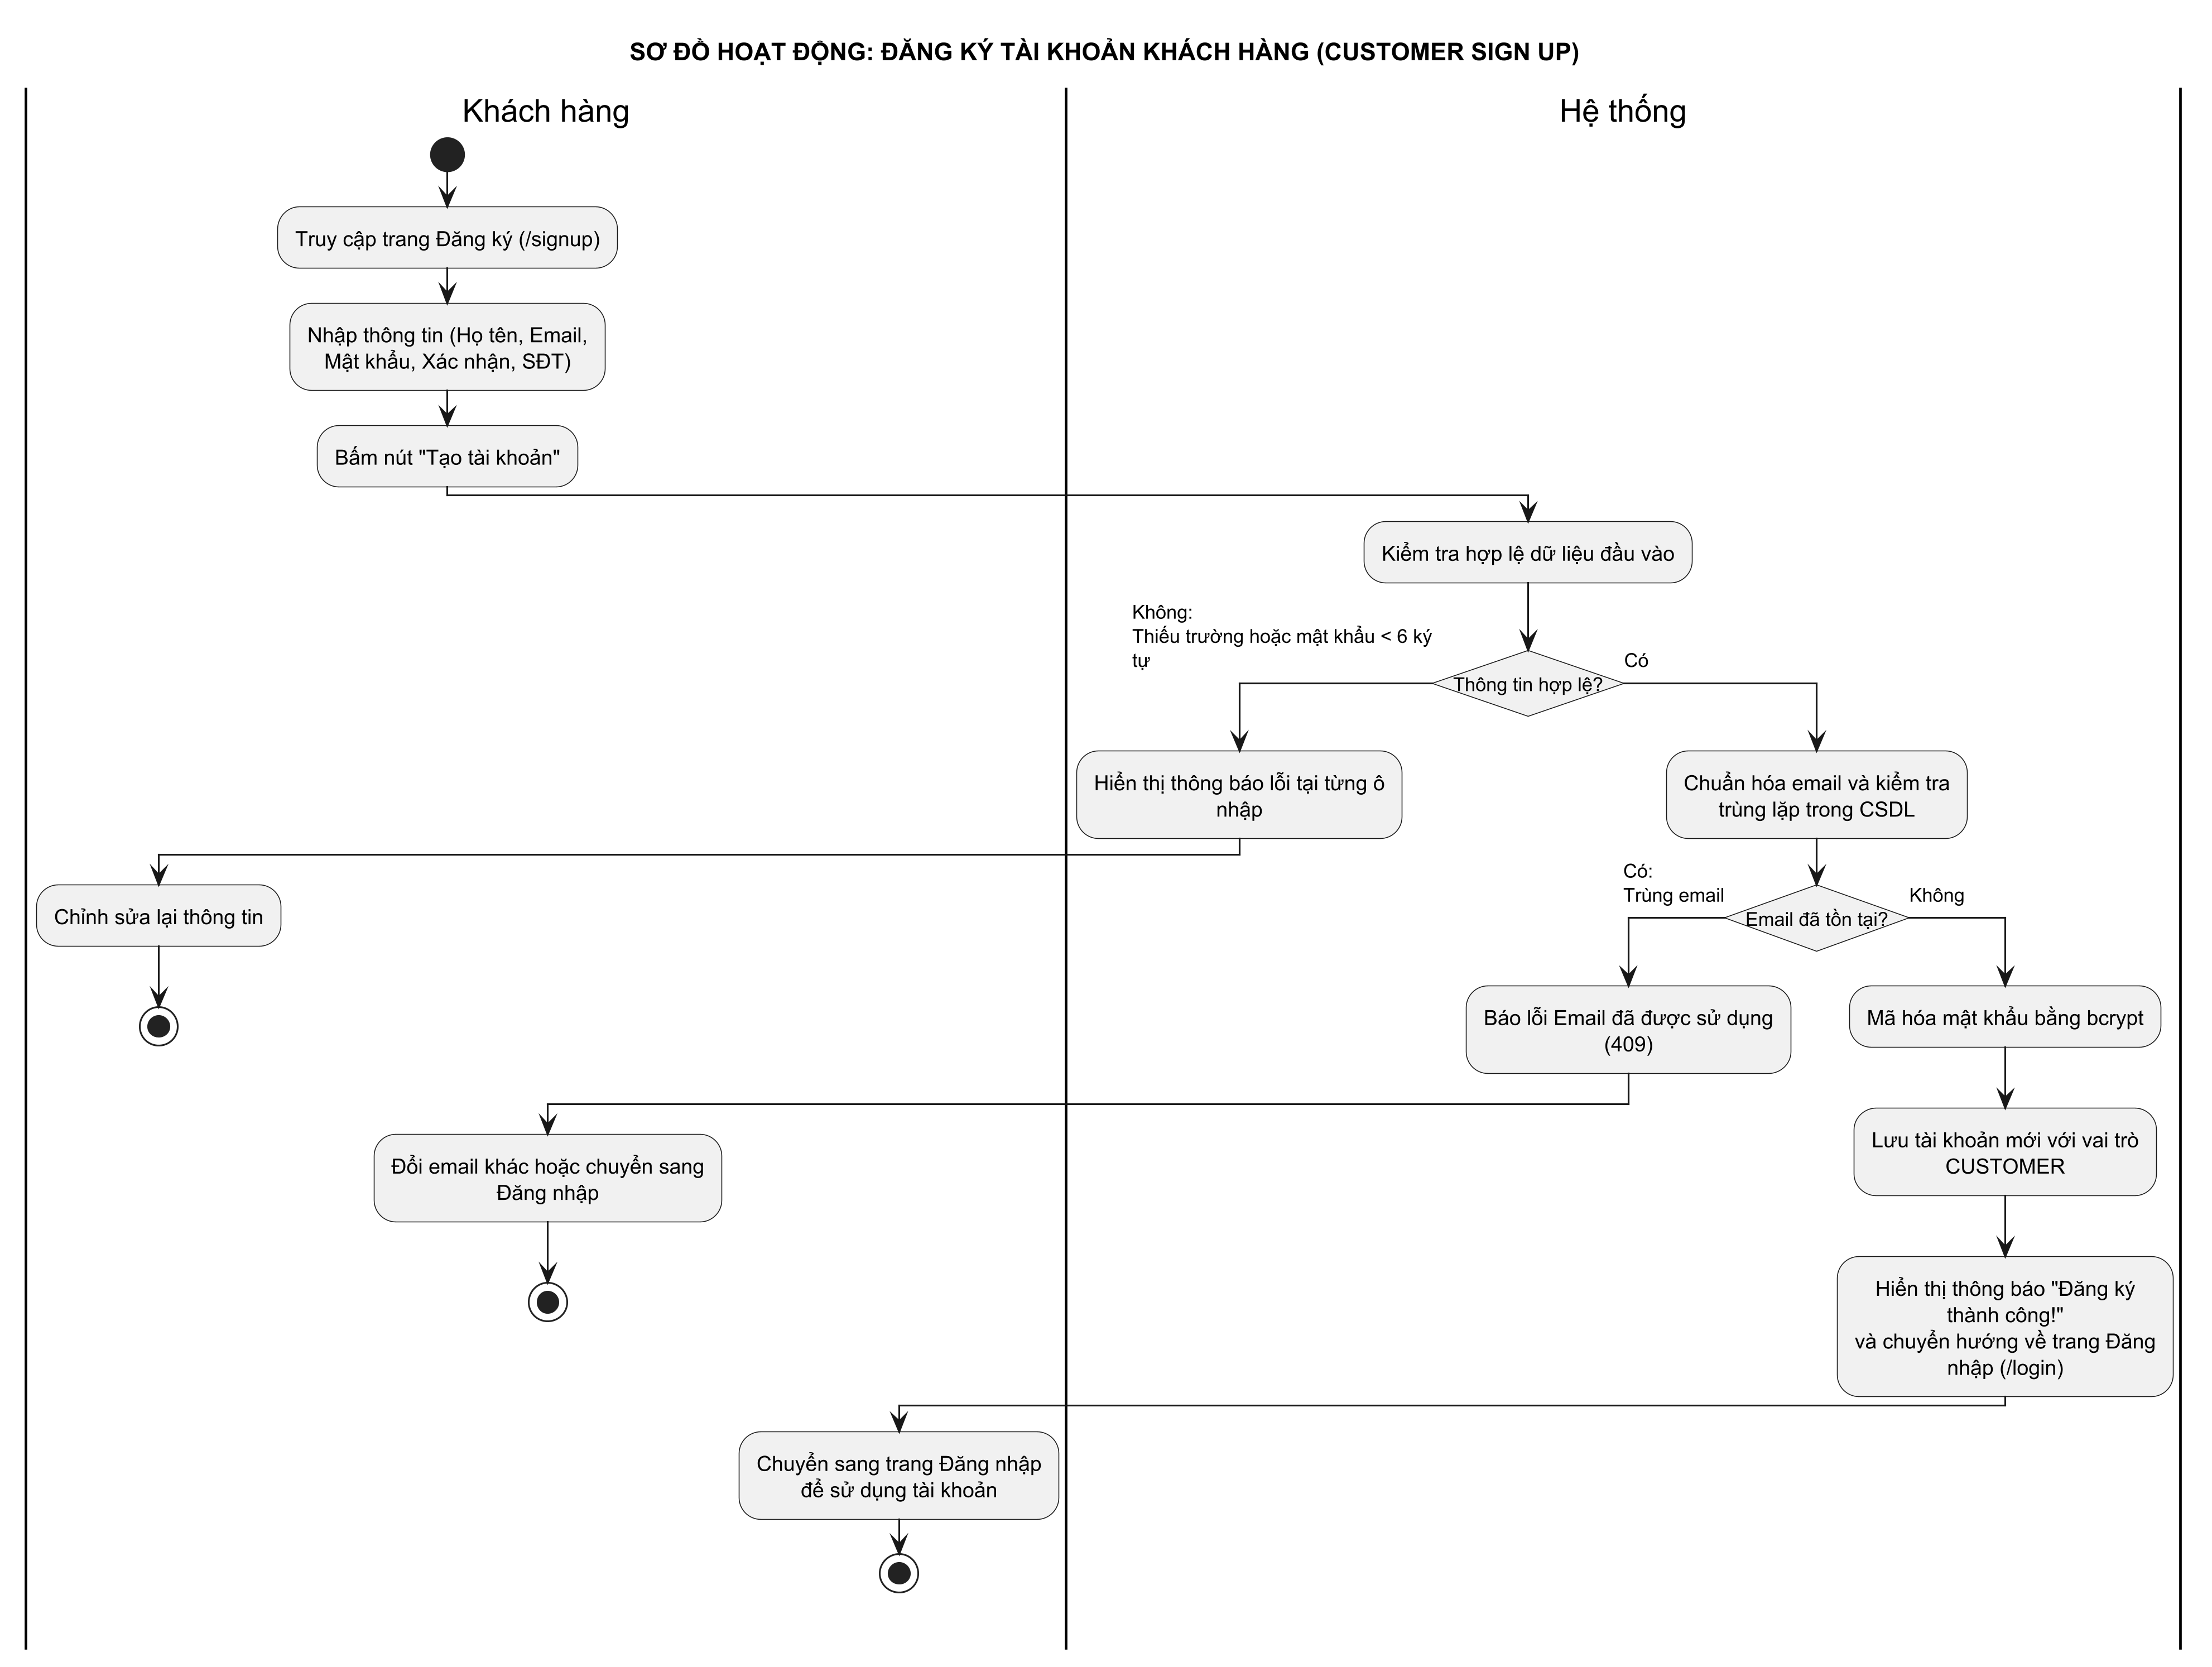
\includegraphics[width=\textwidth,height=0.80\textheight,keepaspectratio]{images/activity/02_dang_ky.png}
  \caption{Activity Diagram: SƠ ĐỒ HOẠT ĐỘNG: ĐĂNG KÝ TÀI KHOẢN KHÁCH HÀNG (CUSTOMER SIGN UP)}
  \label{fig:act_02}
\end{figure}

\subsection{SƠ ĐỒ HOẠT ĐỘNG: ĐĂNG XUẤT HỆ THỐNG (LOGOUT / SIGN OUT)}
\begin{figure}[H]
  \centering
  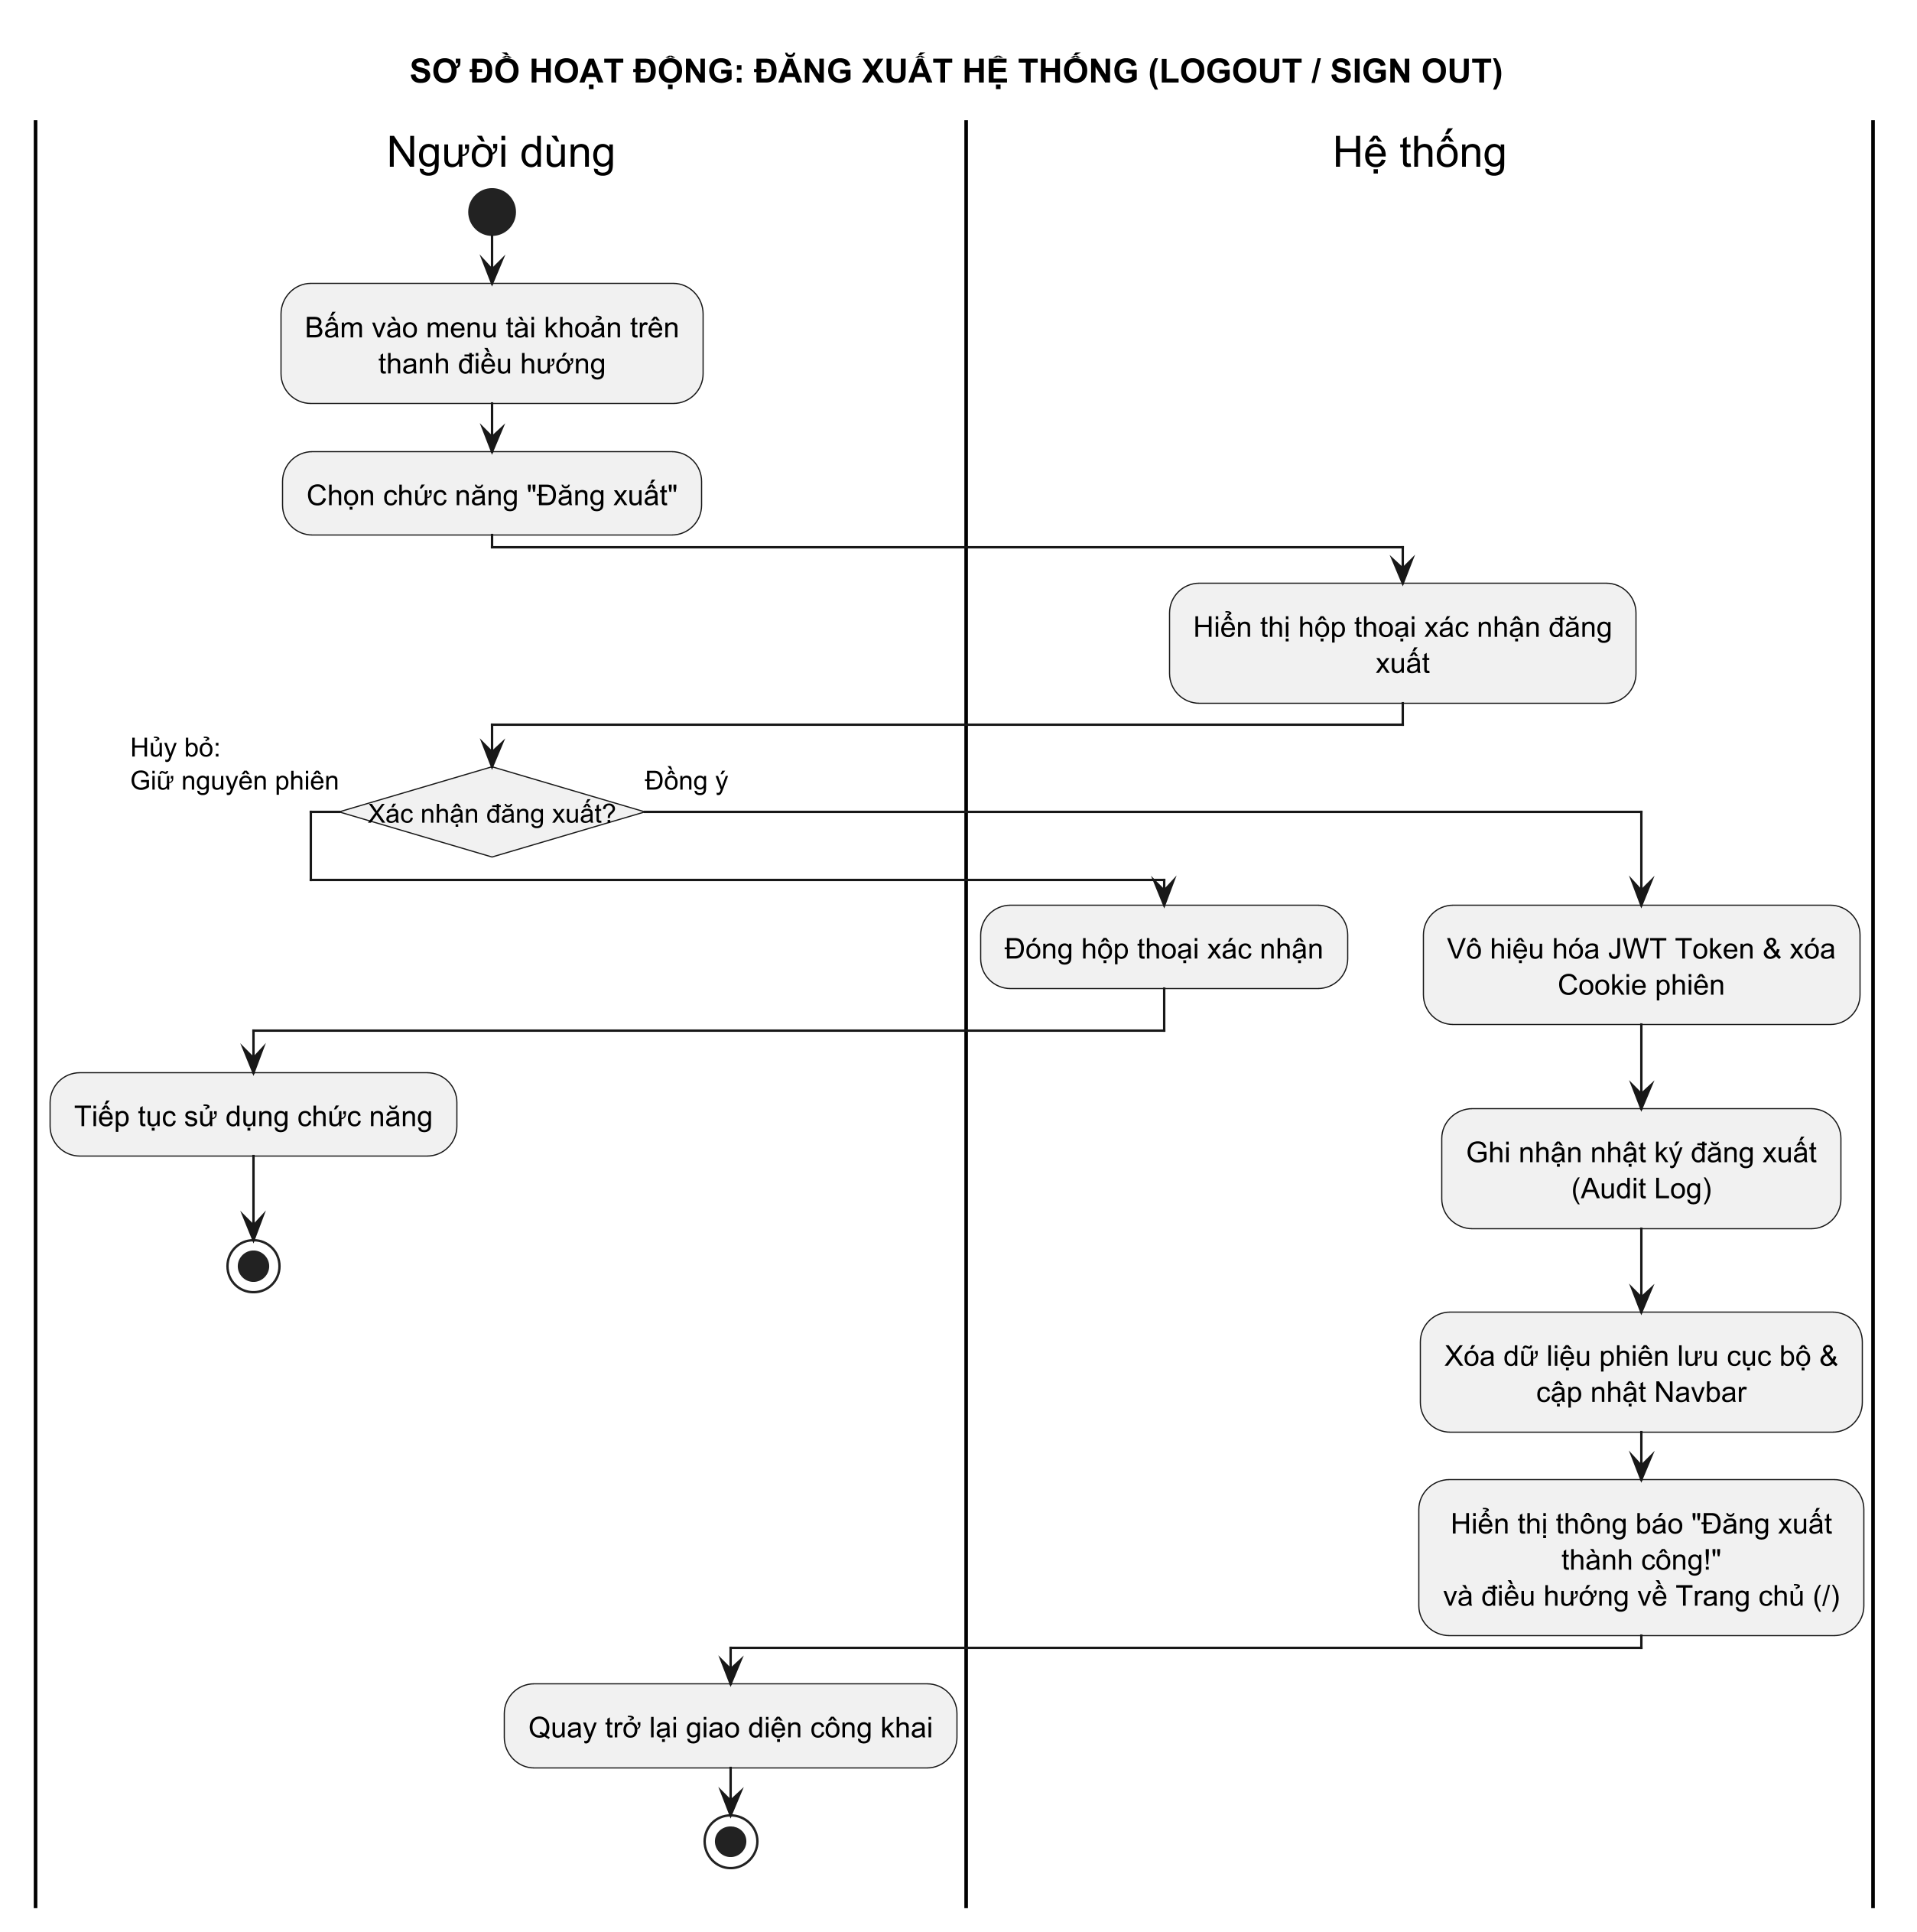
\includegraphics[width=\textwidth,height=0.80\textheight,keepaspectratio]{images/activity/03_dang_xuat.png}
  \caption{Activity Diagram: SƠ ĐỒ HOẠT ĐỘNG: ĐĂNG XUẤT HỆ THỐNG (LOGOUT / SIGN OUT)}
  \label{fig:act_03}
\end{figure}

\subsection{SƠ ĐỒ HOẠT ĐỘNG: ĐÁNH GIÁ VÀ QUẢN LÝ ĐÁNH GIÁ PHIM (MOVIE REVIEWS)}
\begin{figure}[H]
  \centering
  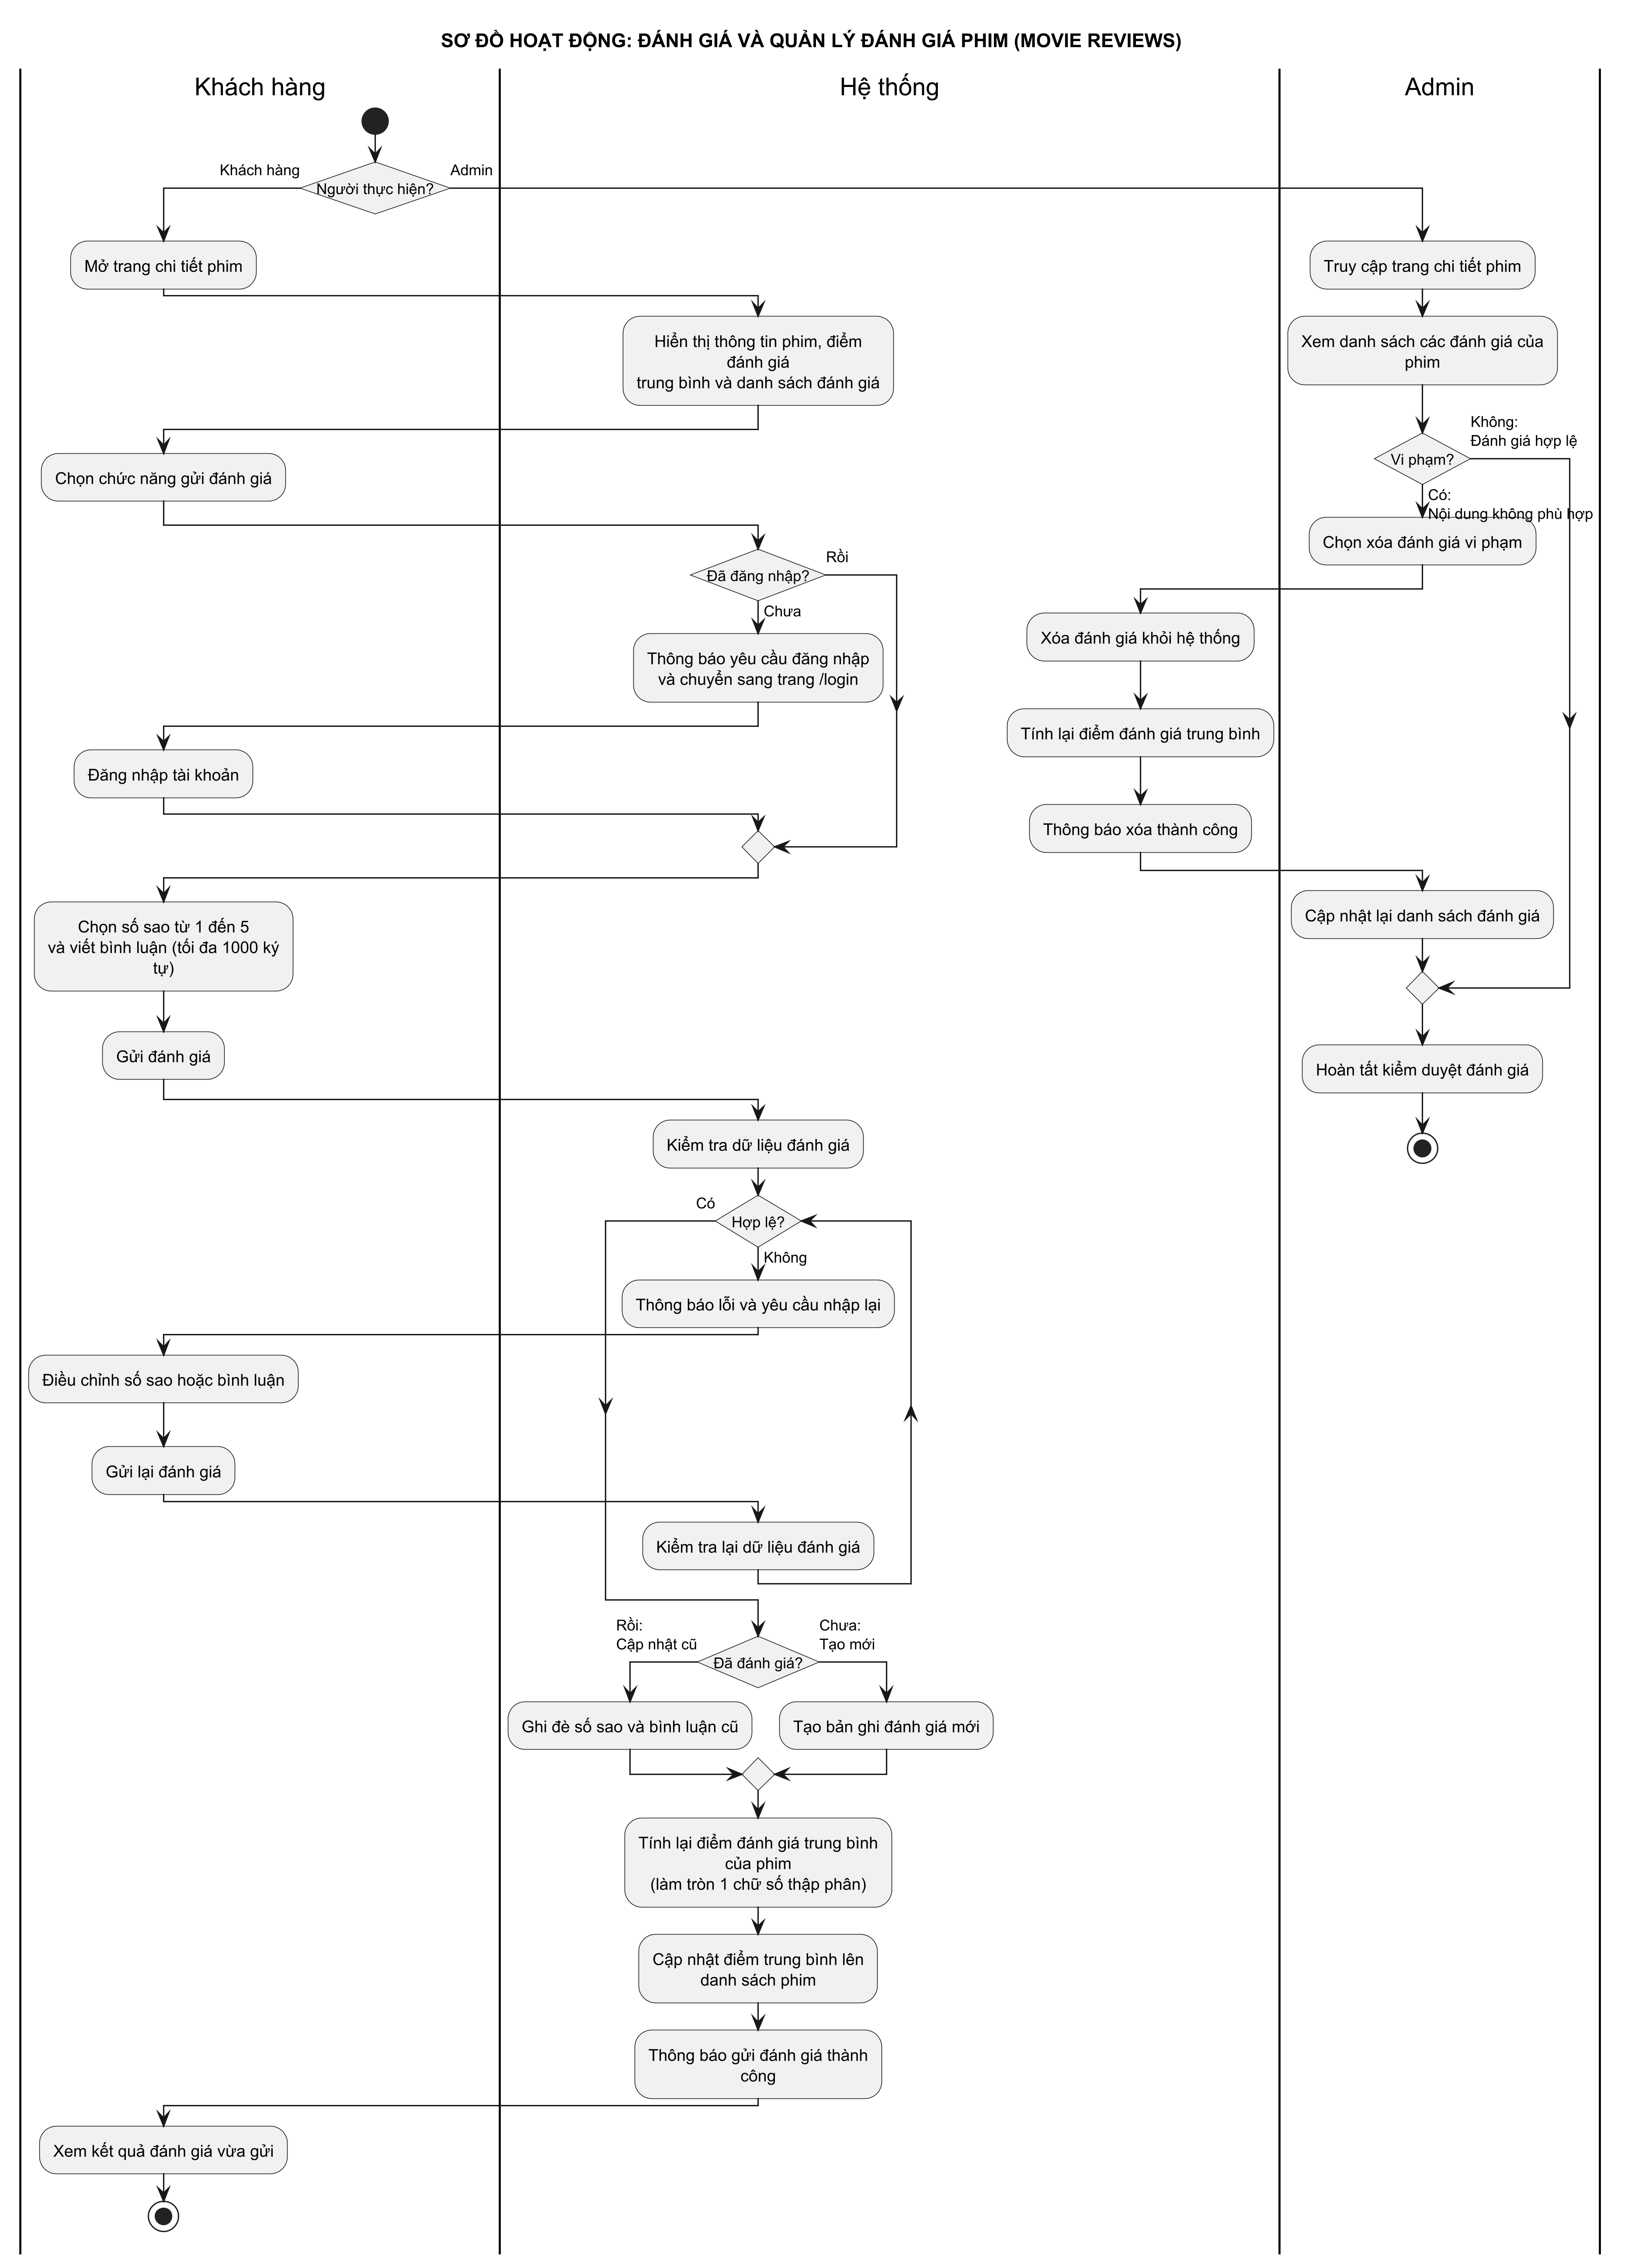
\includegraphics[width=\textwidth,height=0.80\textheight,keepaspectratio]{images/activity/04_danh_gia_phim.png}
  \caption{Activity Diagram: SƠ ĐỒ HOẠT ĐỘNG: ĐÁNH GIÁ VÀ QUẢN LÝ ĐÁNH GIÁ PHIM (MOVIE REVIEWS)}
  \label{fig:act_04}
\end{figure}

\subsection{SƠ ĐỒ HOẠT ĐỘNG: ĐẶT VÉ VÀ MUA COMBO ONLINE (ONLINE TICKET \& COMBO BOOKING)}
\begin{figure}[H]
  \centering
  
\includegraphics[width=\textwidth,height=0.80\textheight,keepaspectratio]{images/activity/05_dat_ve_combo_online.png}
  \caption{Activity Diagram: SƠ ĐỒ HOẠT ĐỘNG: ĐẶT VÉ VÀ MUA COMBO ONLINE (ONLINE TICKET \& COMBO BOOKING)}
  \label{fig:act_05}
\end{figure}

\subsection{SƠ ĐỒ HOẠT ĐỘNG: BÁN VÉ TẠI QUẦY (POS TICKET SALES)}
\begin{figure}[H]
  \centering
  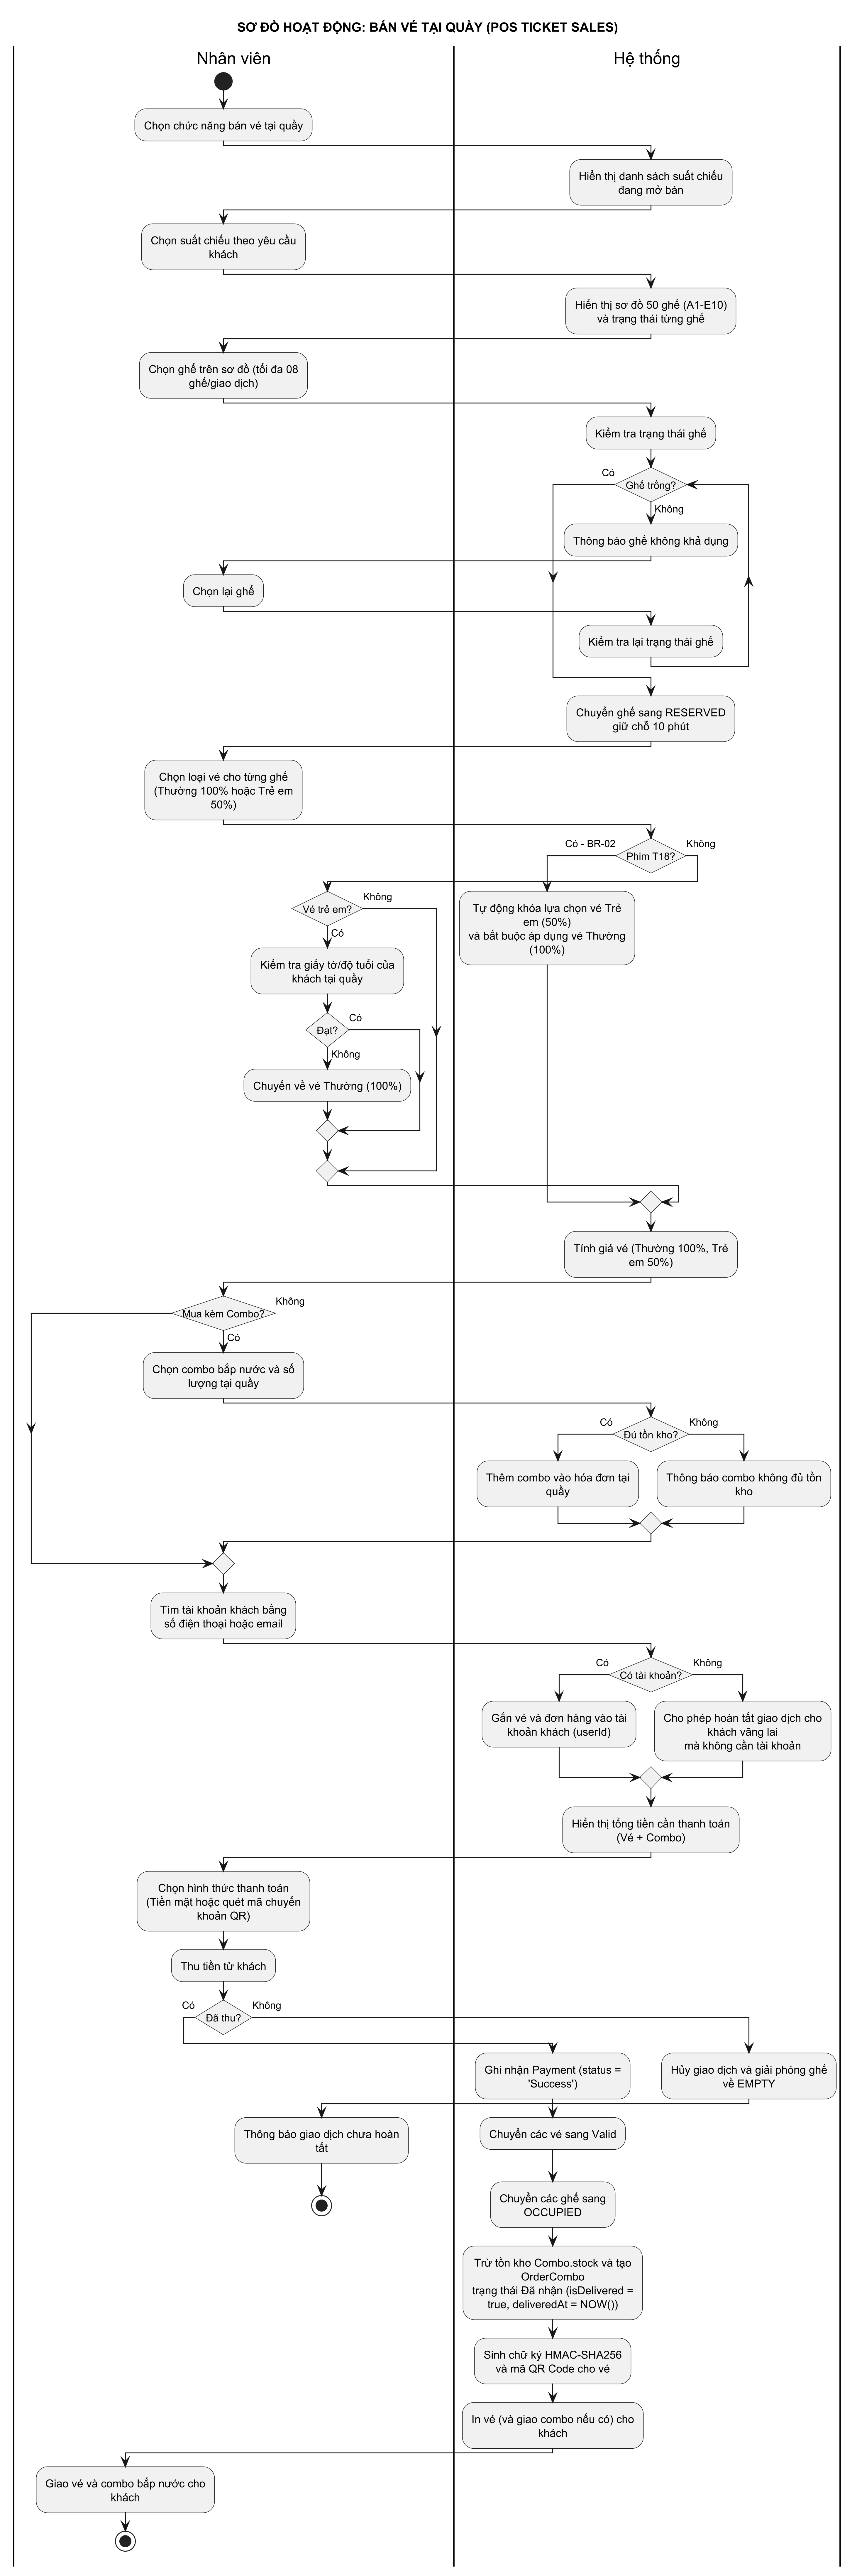
\includegraphics[width=\textwidth,height=0.80\textheight,keepaspectratio]{images/activity/06_ban_ve_tai_quay.png}
  \caption{Activity Diagram: SƠ ĐỒ HOẠT ĐỘNG: BÁN VÉ TẠI QUẦY (POS TICKET SALES)}
  \label{fig:act_06}
\end{figure}

\subsection{SƠ ĐỒ HOẠT ĐỘNG: BÁN COMBO BẮP NƯỚC TẠI QUẦY (POS COMBO SALES)}
\begin{figure}[H]
  \centering
  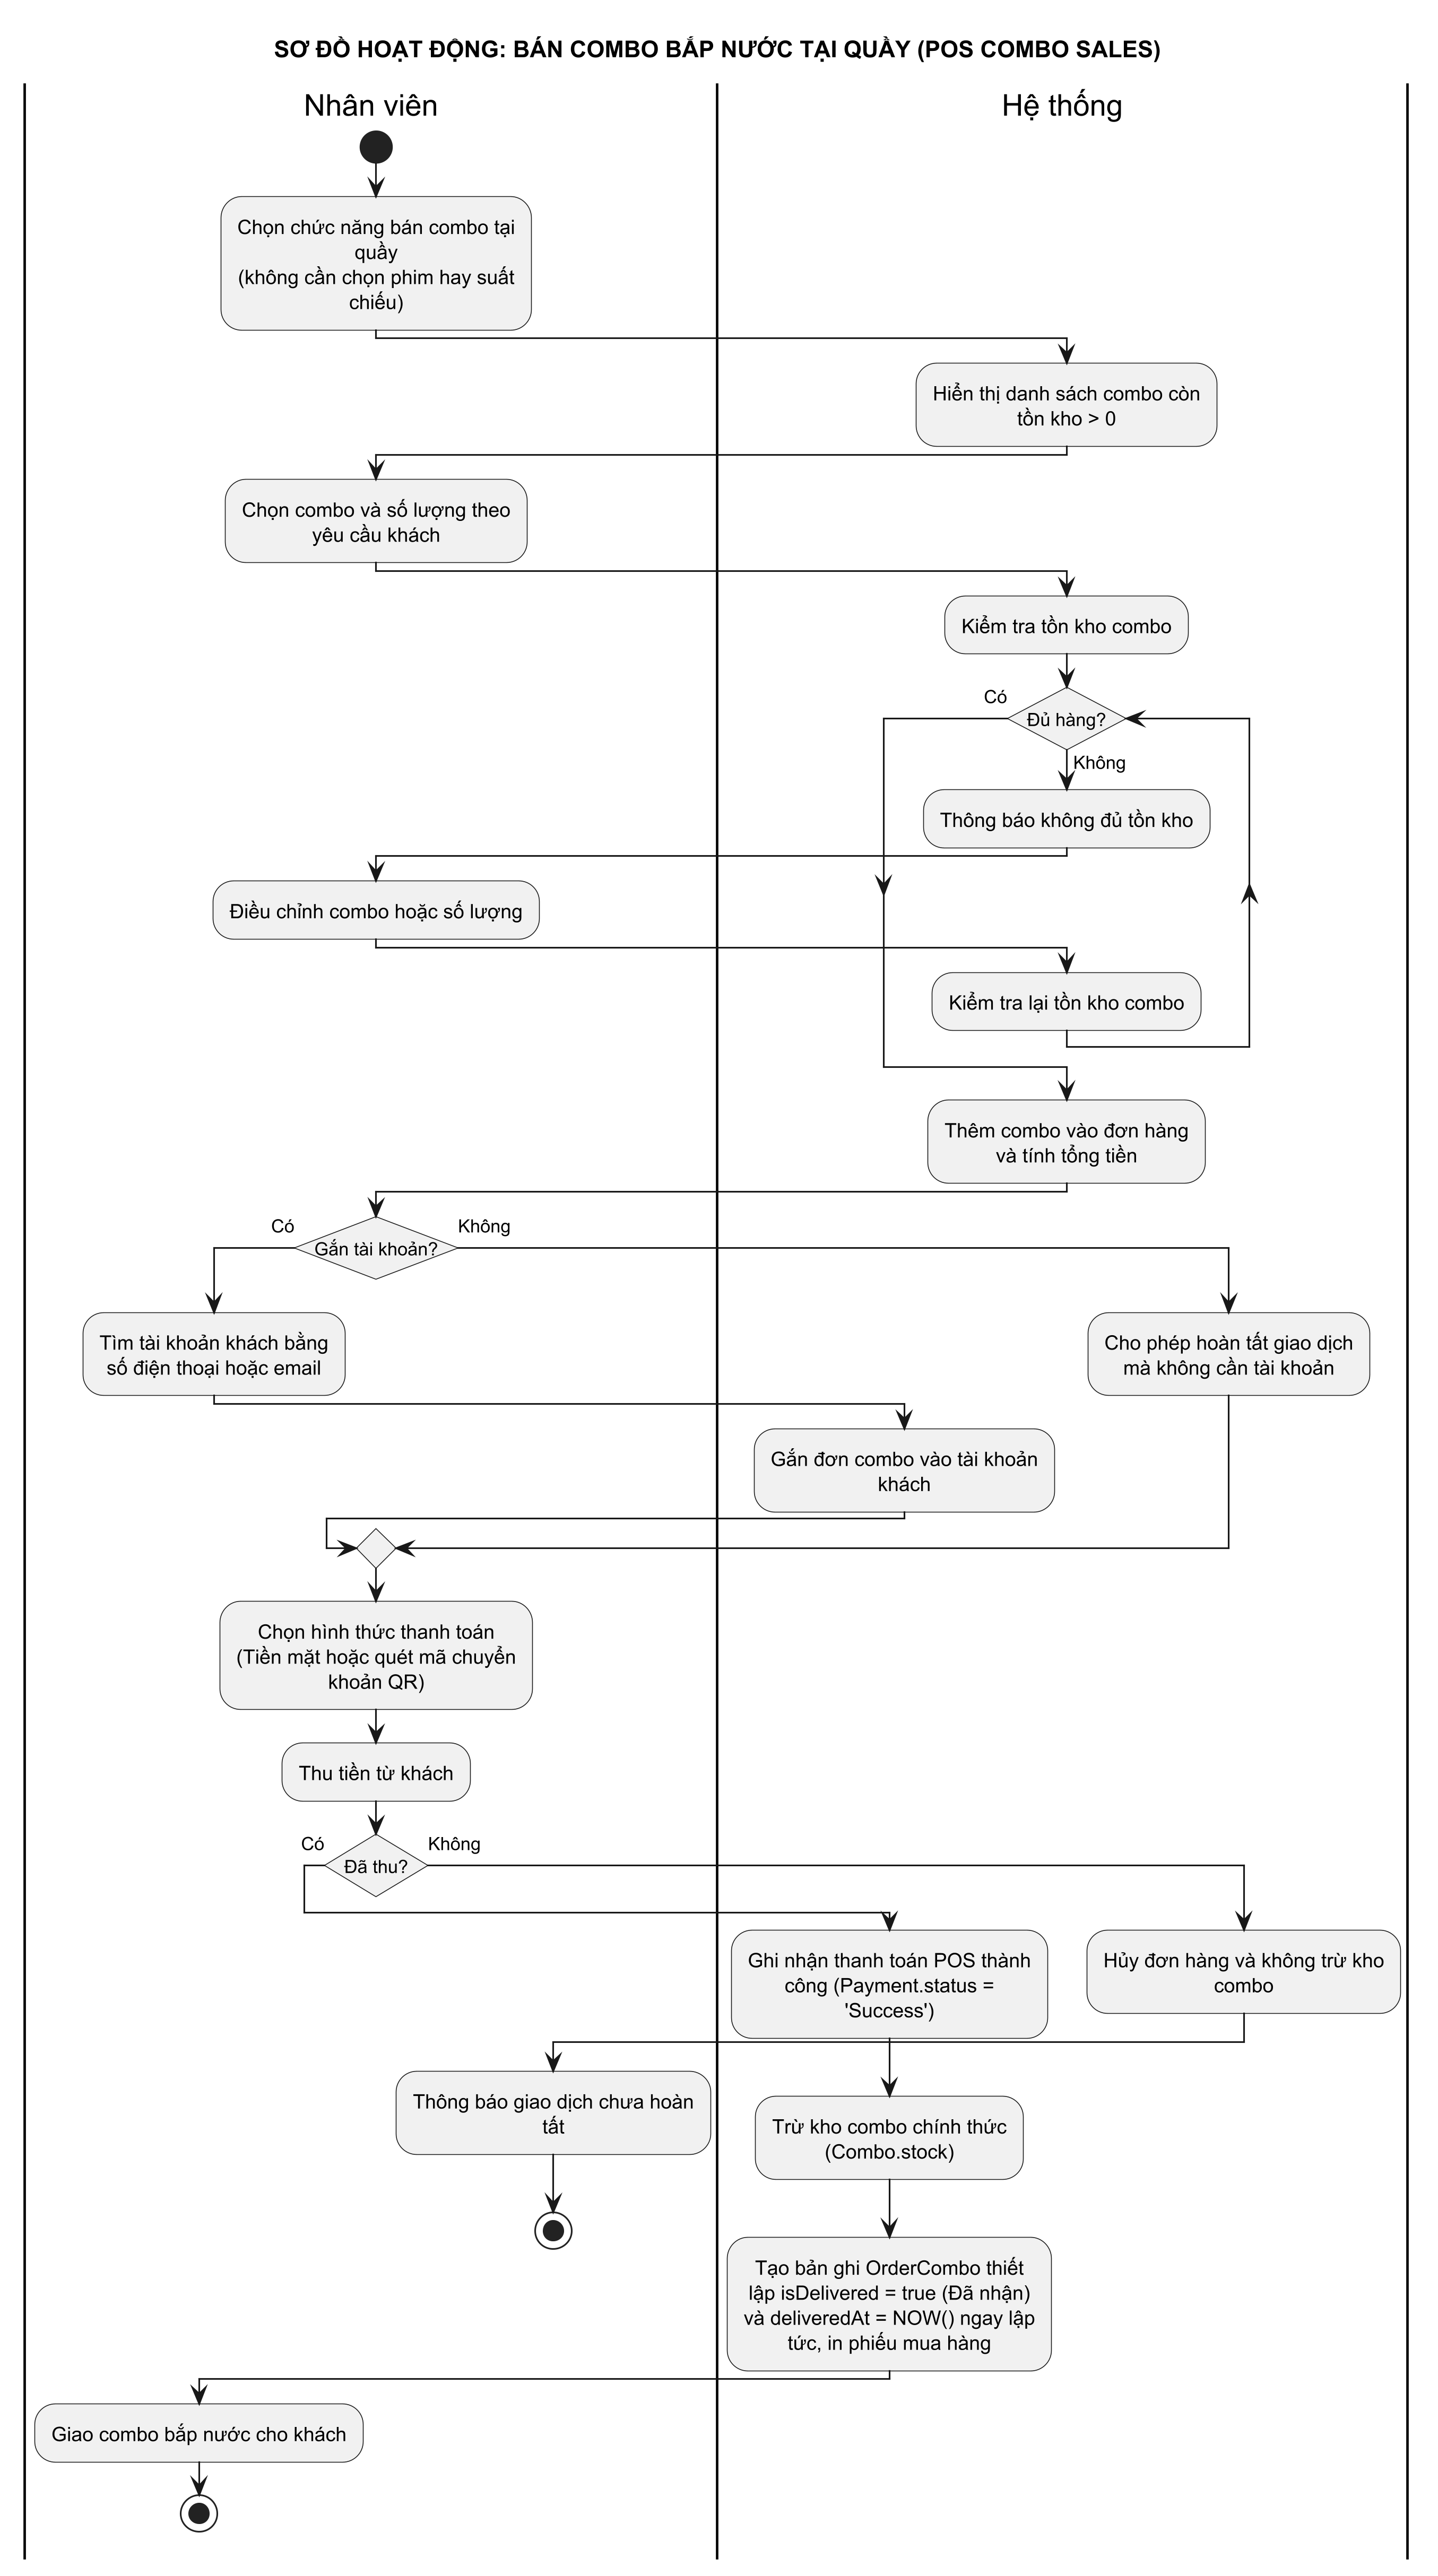
\includegraphics[width=\textwidth,height=0.80\textheight,keepaspectratio]{images/activity/07_ban_combo_tai_quay.png}
  \caption{Activity Diagram: SƠ ĐỒ HOẠT ĐỘNG: BÁN COMBO BẮP NƯỚC TẠI QUẦY (POS COMBO SALES)}
  \label{fig:act_07}
\end{figure}

\subsection{SƠ ĐỒ HOẠT ĐỘNG: SOÁT VÉ VÀO RẠP (TICKET CHECK-IN)}
\begin{figure}[H]
  \centering
  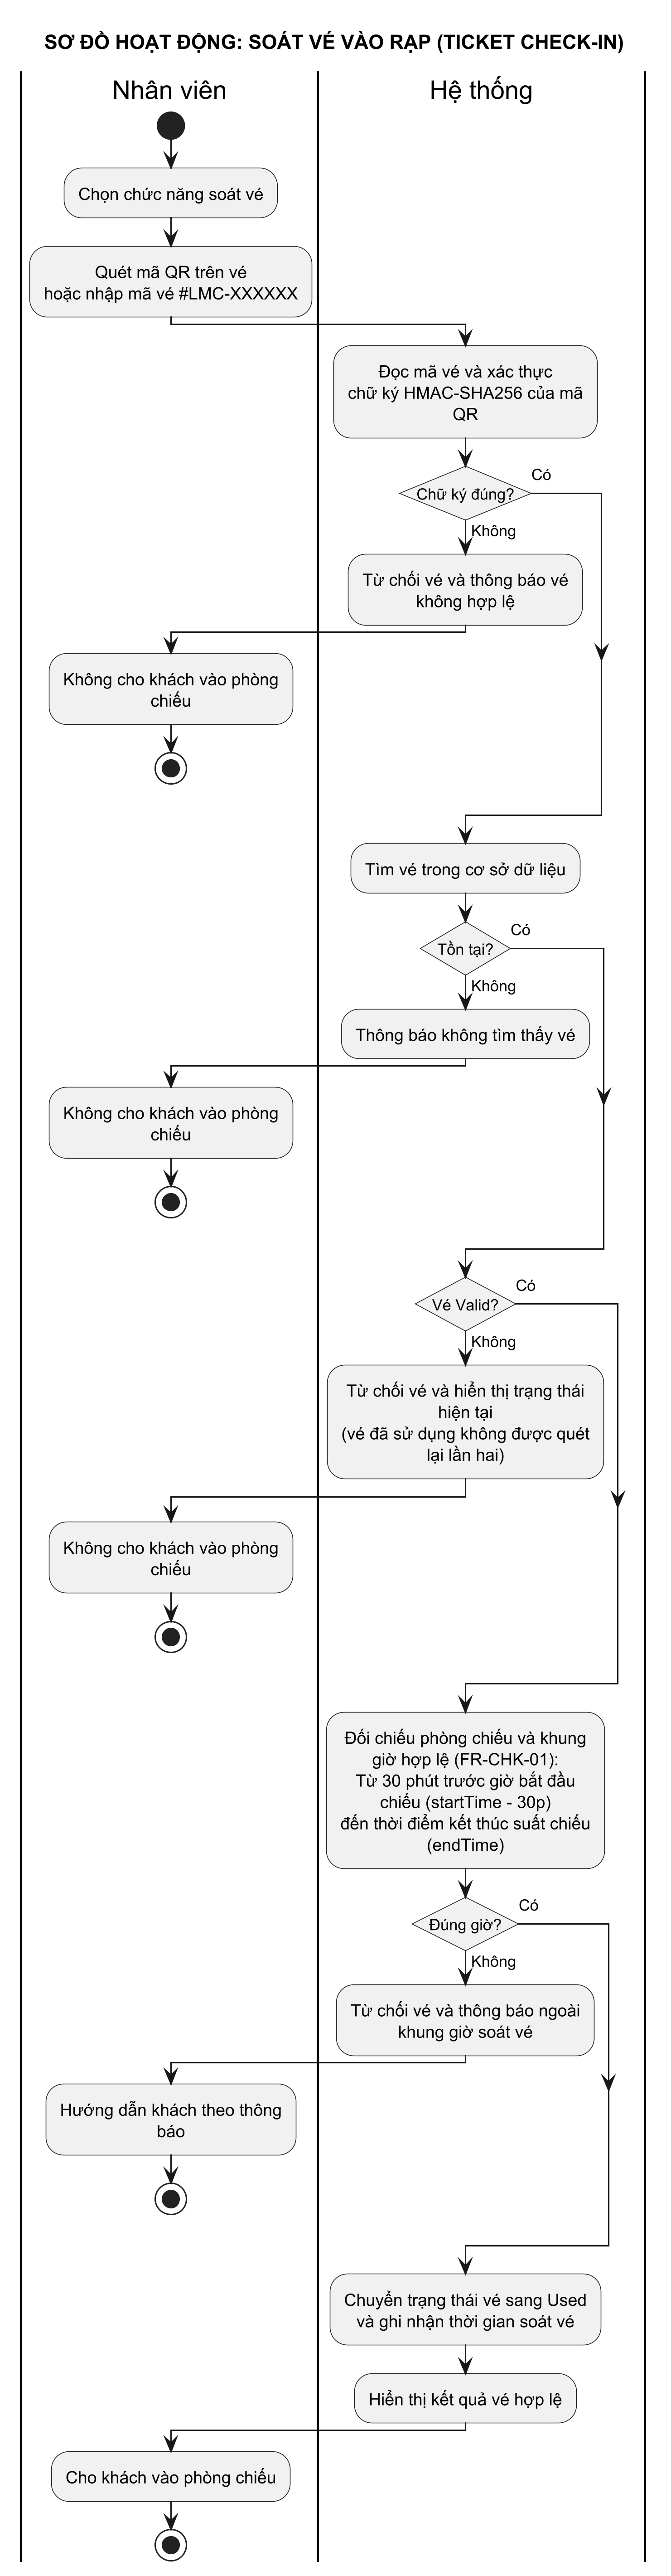
\includegraphics[width=\textwidth,height=0.80\textheight,keepaspectratio]{images/activity/08_soat_ve.png}
  \caption{Activity Diagram: SƠ ĐỒ HOẠT ĐỘNG: SOÁT VÉ VÀO RẠP (TICKET CHECK-IN)}
  \label{fig:act_08}
\end{figure}

\subsection{SƠ ĐỒ HOẠT ĐỘNG: GIAO NHẬN COMBO ĐÃ ĐẶT ONLINE (COMBO FULFILLMENT)}
\begin{figure}[H]
  \centering
  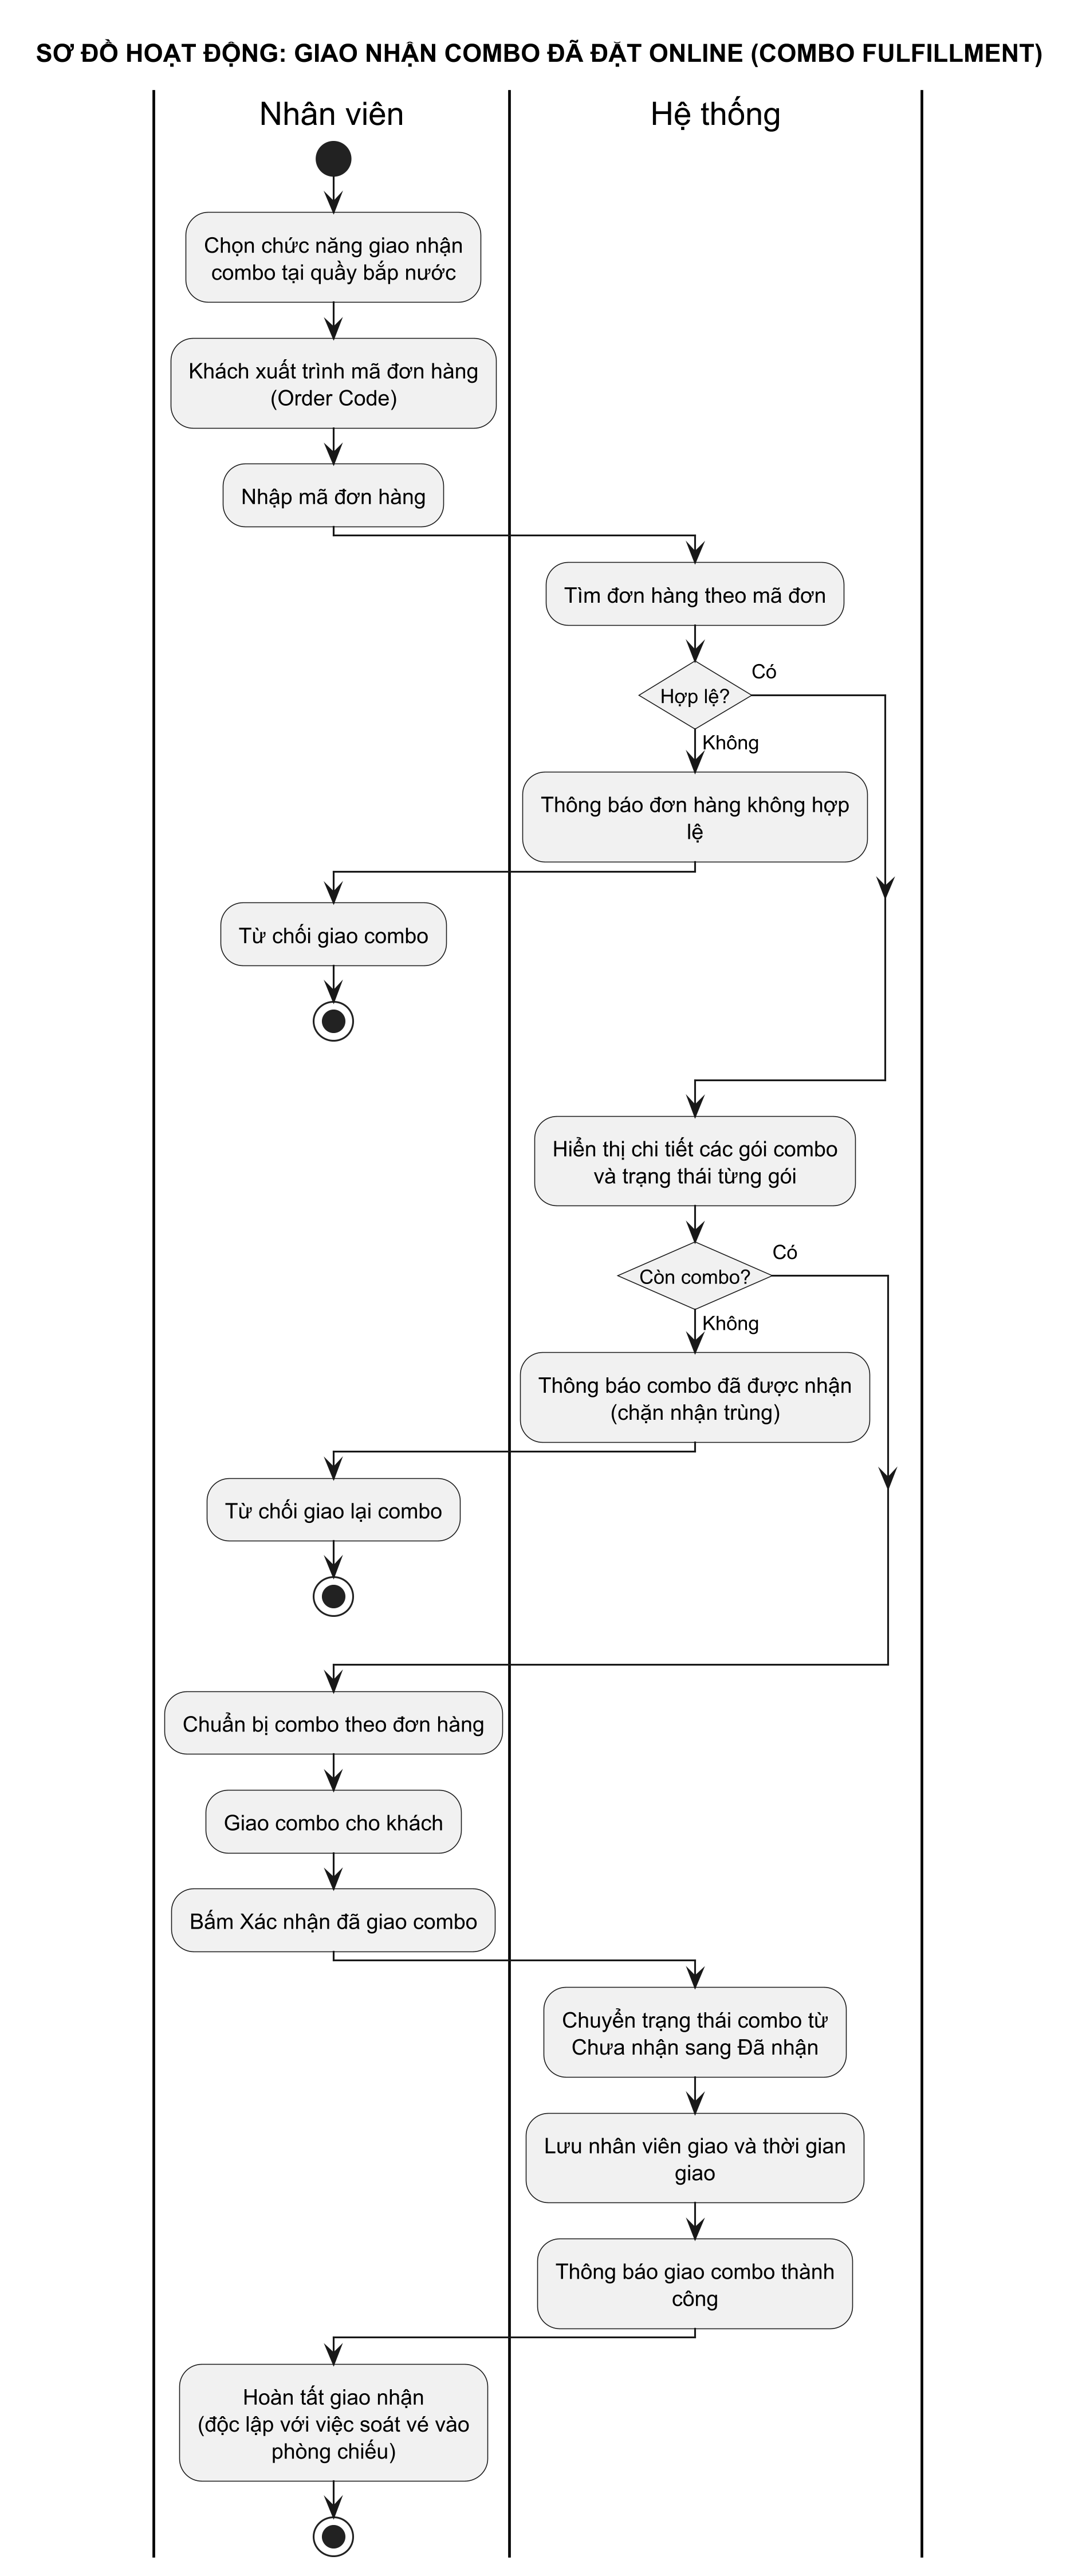
\includegraphics[width=\textwidth,height=0.80\textheight,keepaspectratio]{images/activity/09_giao_nhan_combo.png}
  \caption{Activity Diagram: SƠ ĐỒ HOẠT ĐỘNG: GIAO NHẬN COMBO ĐÃ ĐẶT ONLINE (COMBO FULFILLMENT)}
  \label{fig:act_09}
\end{figure}

\subsection{SƠ ĐỒ HOẠT ĐỘNG: KHÁCH HỦY VÉ VÀ CẤP VOUCHER 50\% (CUSTOMER TICKET CANCELLATION - BR-03 \& FR-CAN-01)}
\begin{figure}[H]
  \centering
  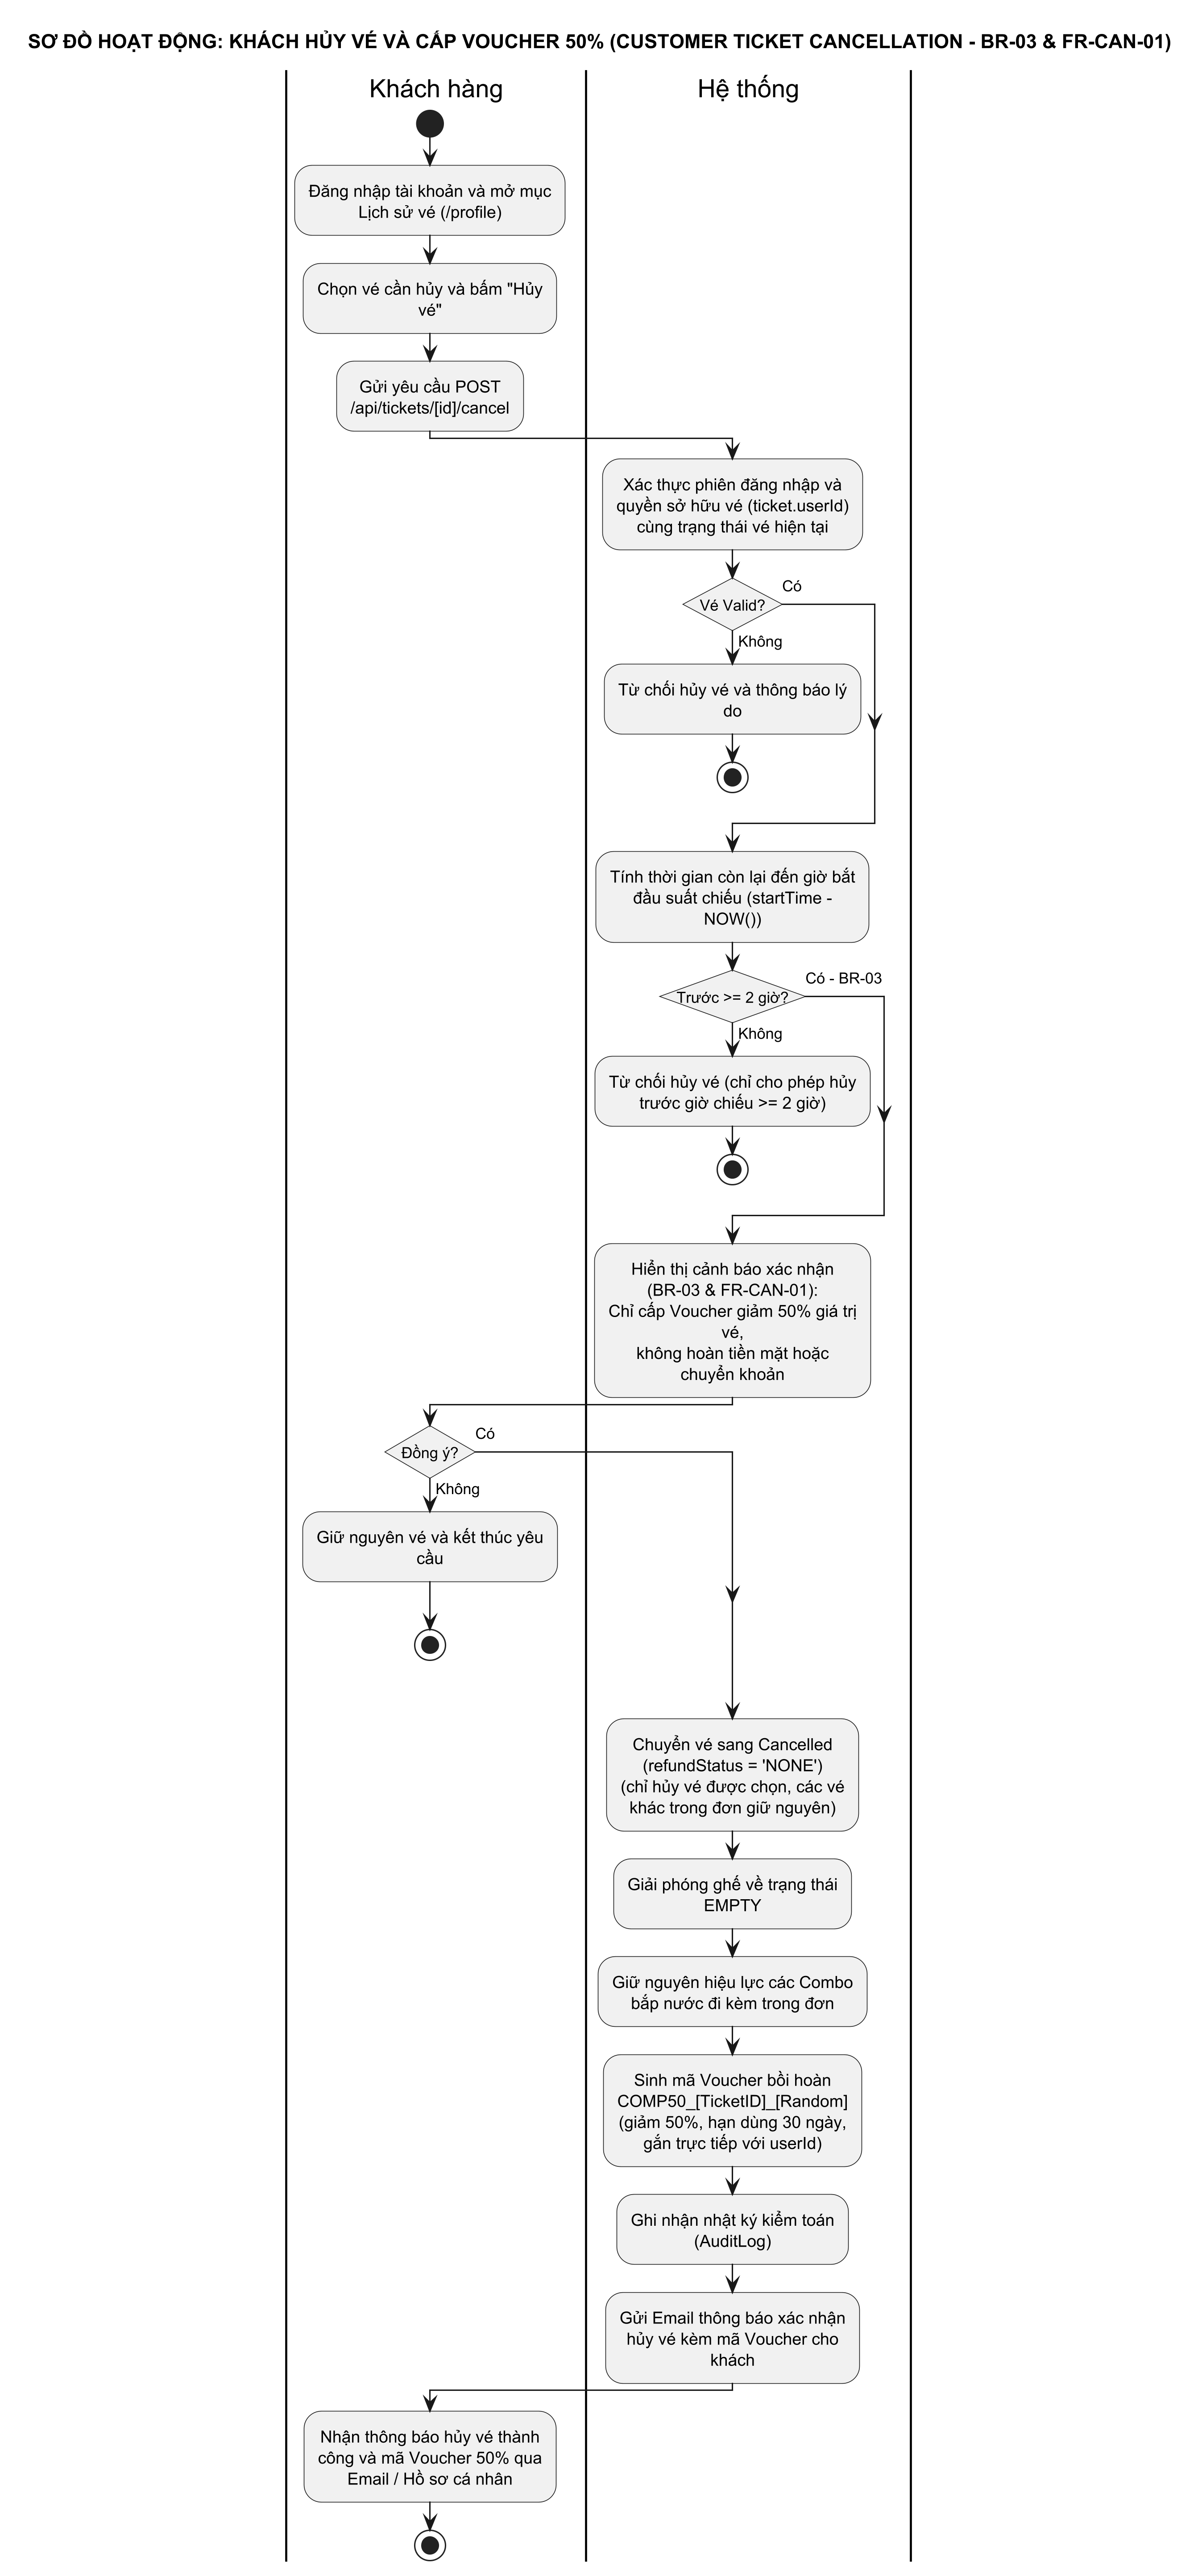
\includegraphics[width=\textwidth,height=0.80\textheight,keepaspectratio]{images/activity/10_khach_huy_ve.png}
  \caption{Activity Diagram: SƠ ĐỒ HOẠT ĐỘNG: KHÁCH HỦY VÉ VÀ CẤP VOUCHER 50\% (CUSTOMER TICKET CANCELLATION - BR-03 \& FR-CAN-01)}
  \label{fig:act_10}
\end{figure}

\subsection{SƠ ĐỒ HOẠT ĐỘNG: RẠP HỦY VÉ \& BỒI HOÀN 1 BƯỚC (CASH 100\% / VOUCHER 100\%)}
\begin{figure}[H]
  \centering
  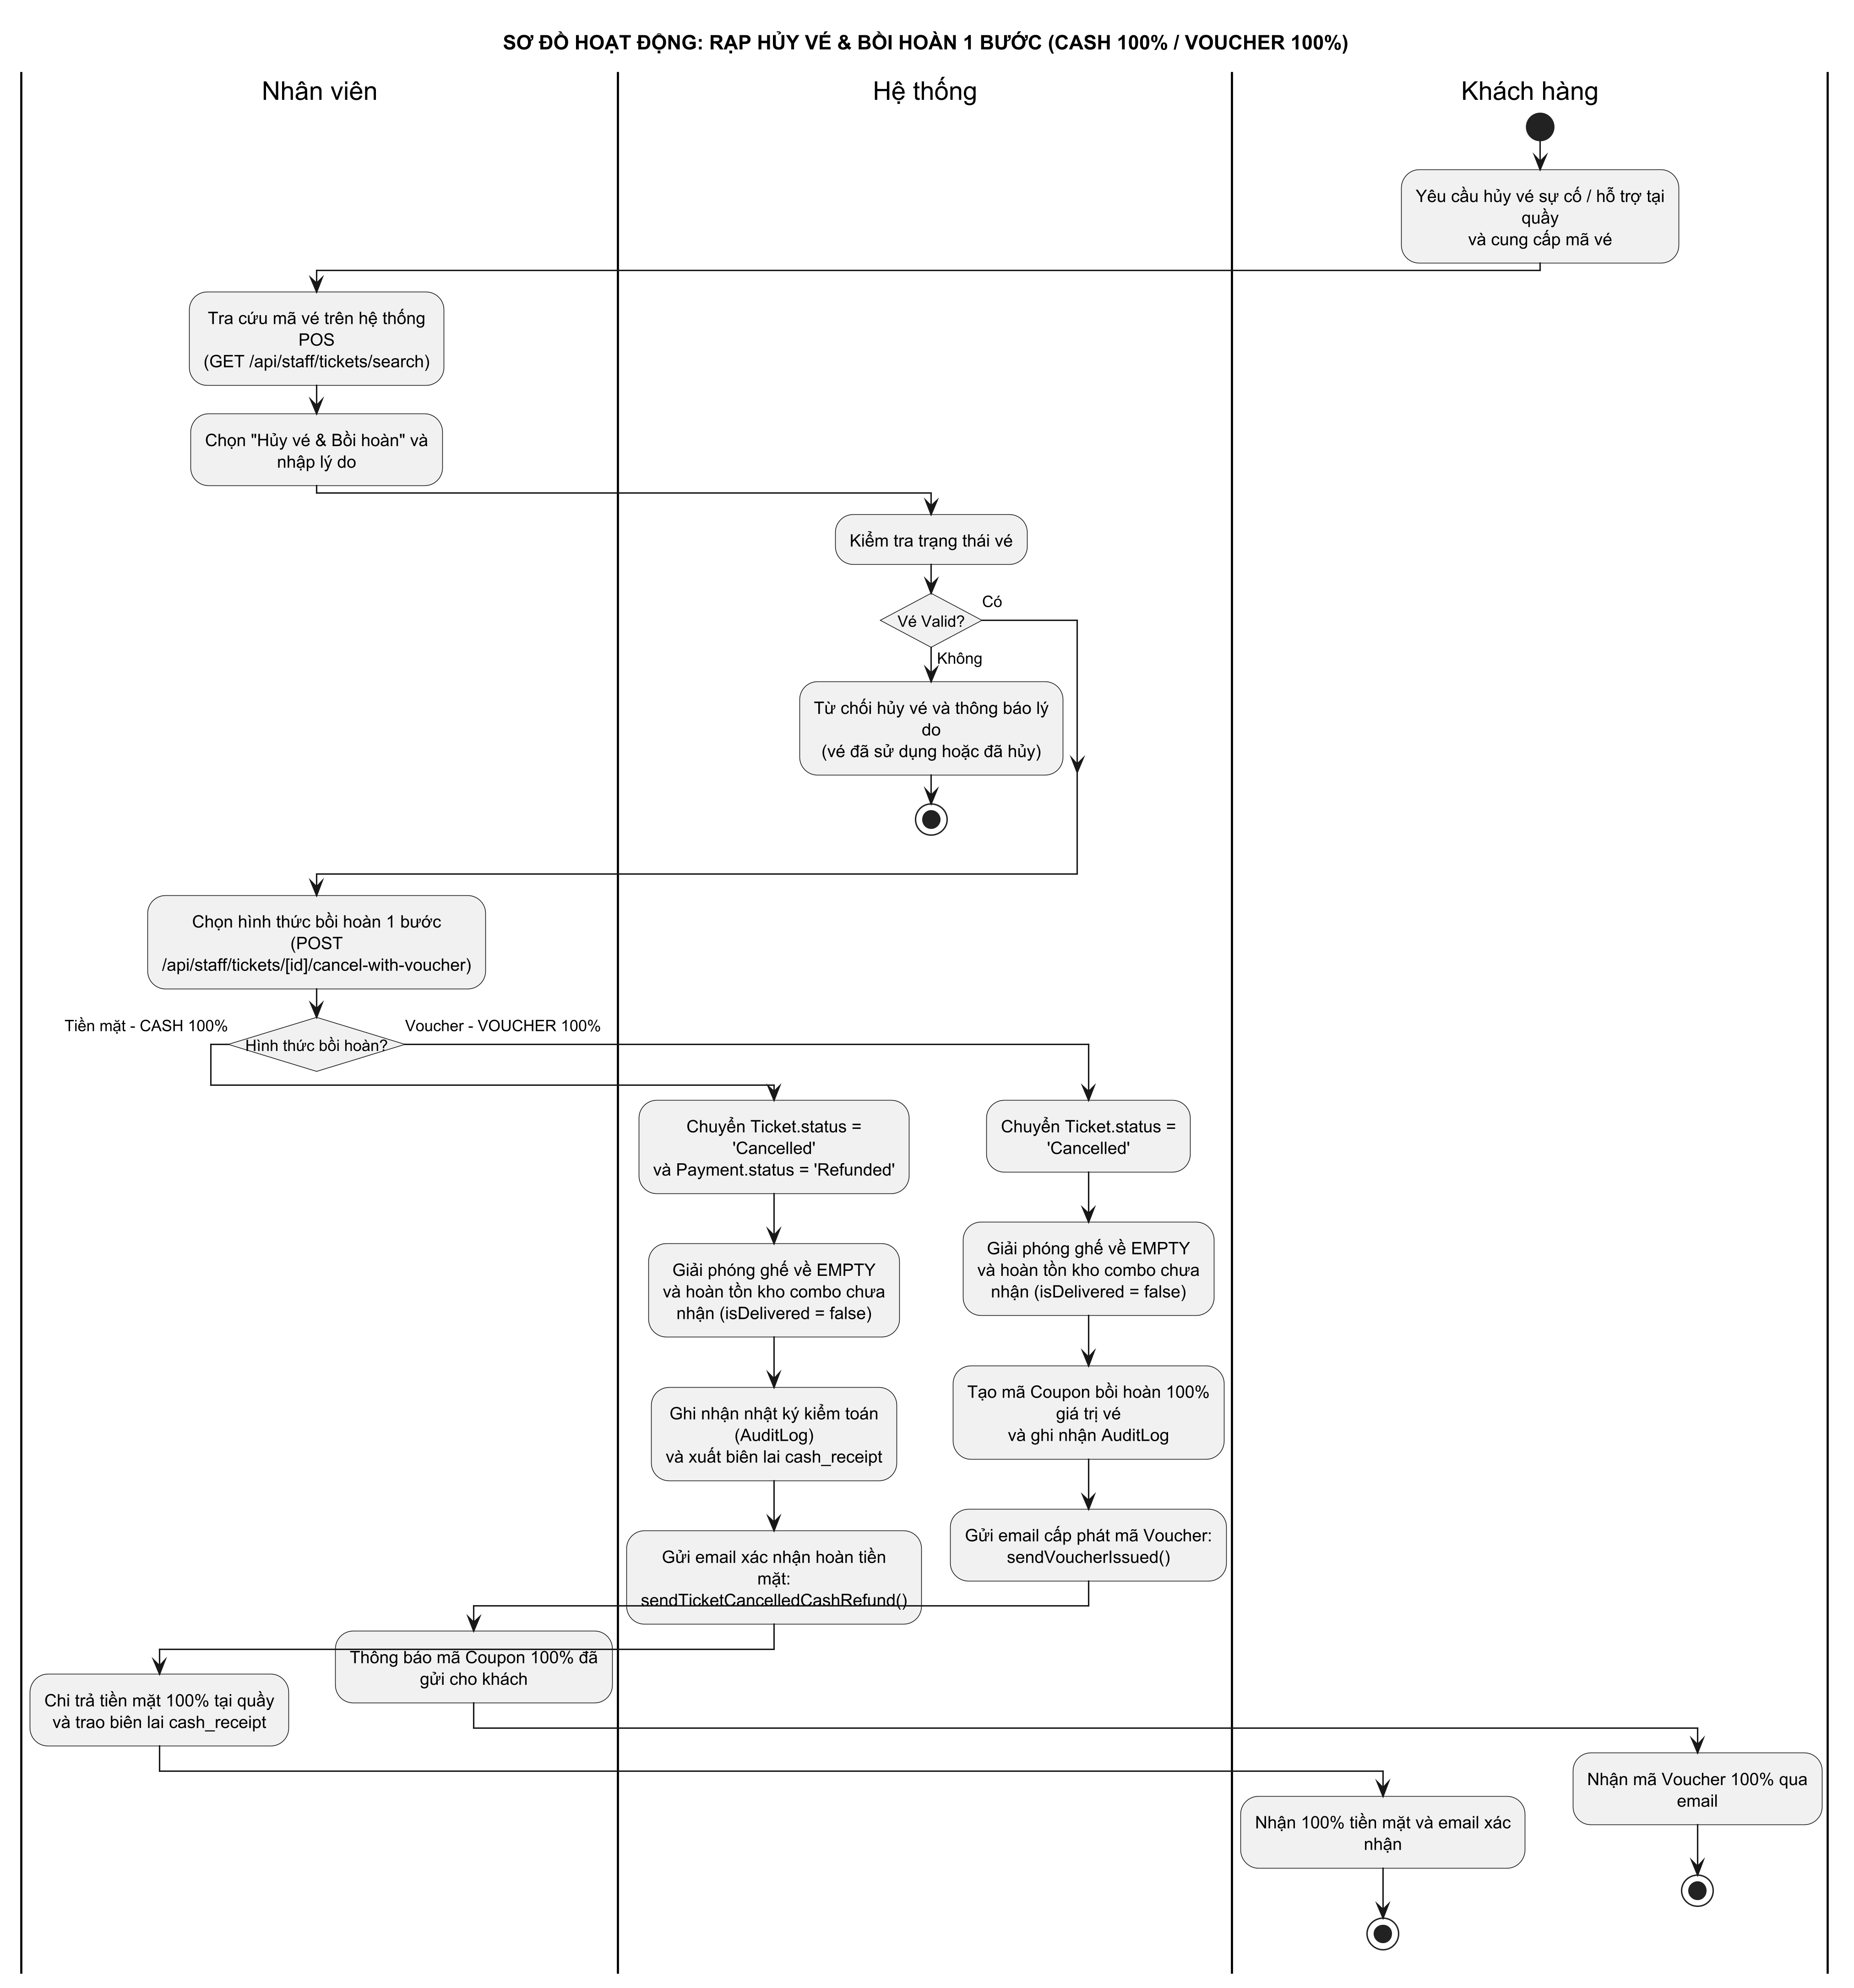
\includegraphics[width=\textwidth,height=0.80\textheight,keepaspectratio]{images/activity/11_rap_huy_ve_hoan_tien.png}
  \caption{Activity Diagram: SƠ ĐỒ HOẠT ĐỘNG: RẠP HỦY VÉ \& BỒI HOÀN 1 BƯỚC (CASH 100\% / VOUCHER 100\%)}
  \label{fig:act_11}
\end{figure}

\subsection{SƠ ĐỒ HOẠT ĐỘNG: QUẢN LÝ VOUCHER KHUYẾN MÃI (VOUCHER MANAGEMENT)}
\begin{figure}[H]
  \centering
  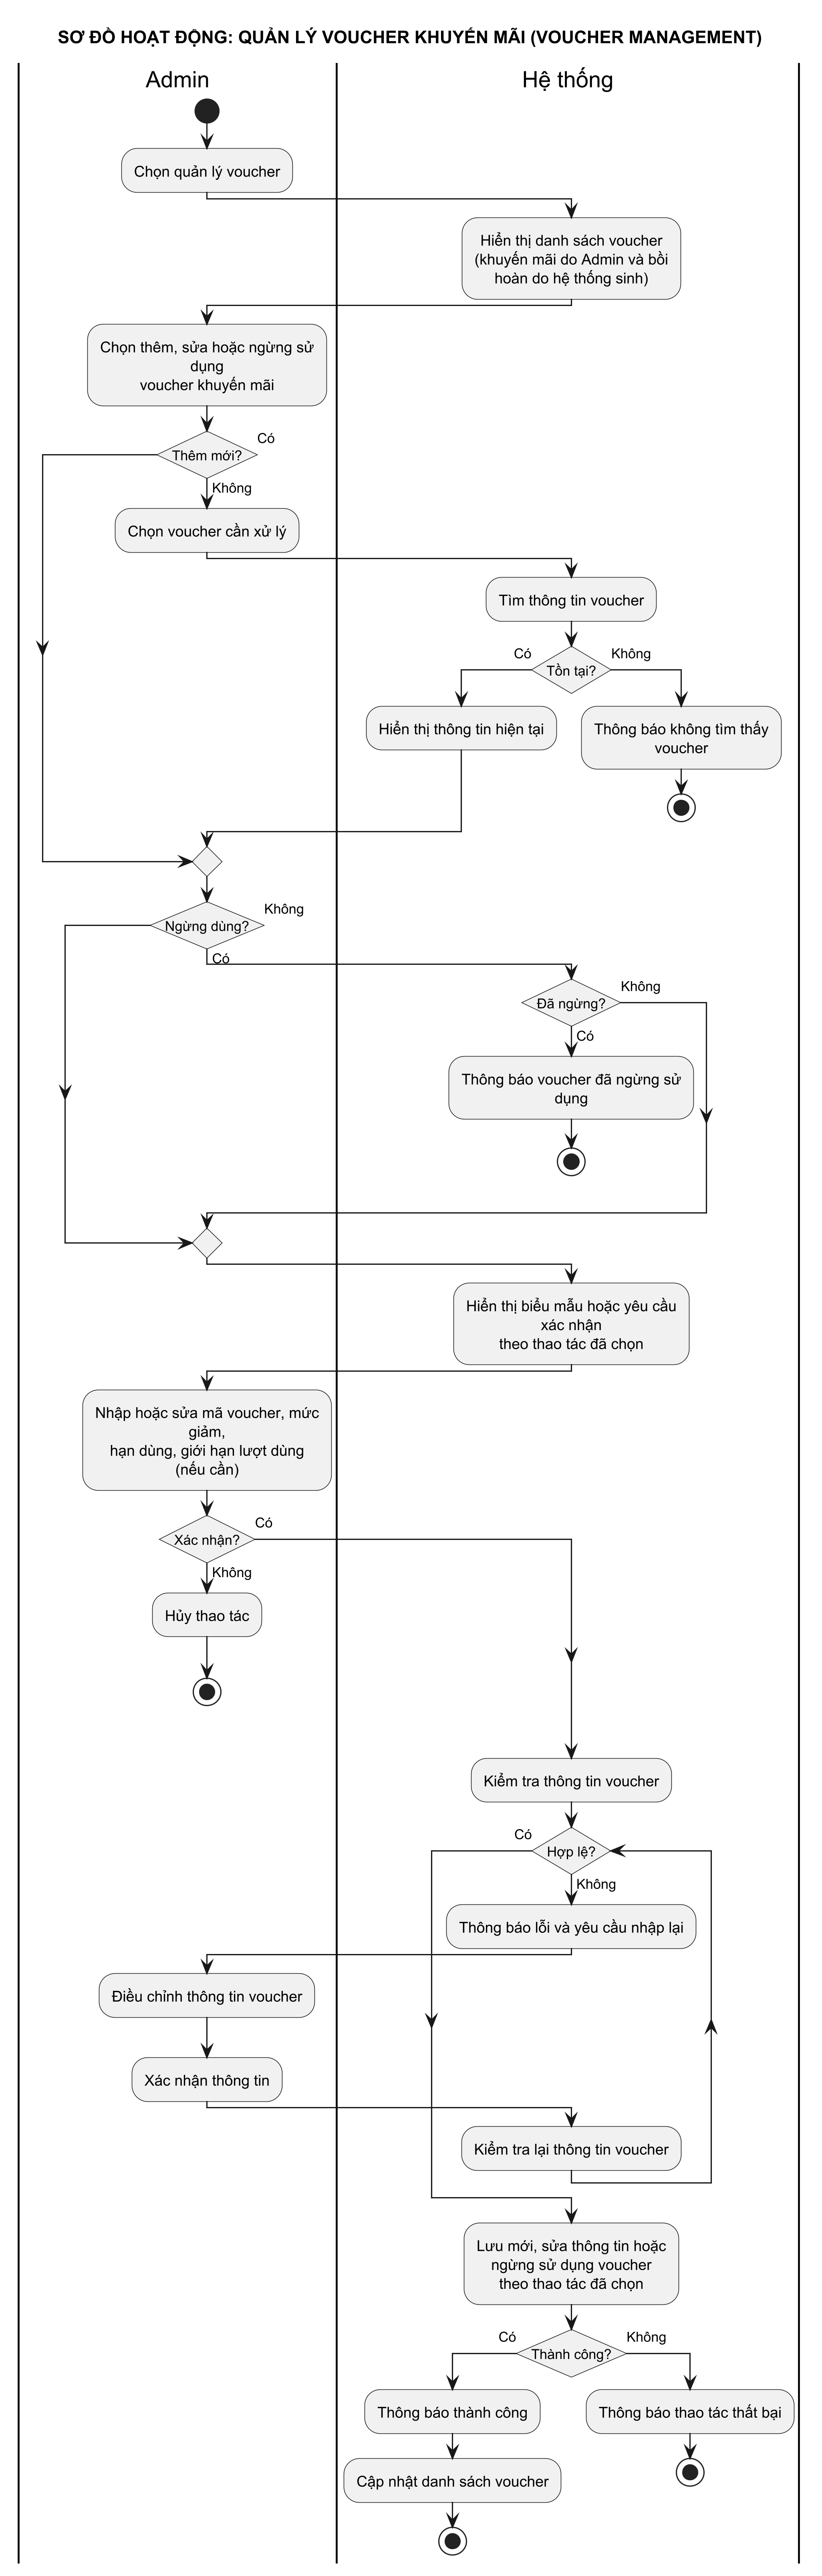
\includegraphics[width=\textwidth,height=0.80\textheight,keepaspectratio]{images/activity/12_quan_ly_voucher.png}
  \caption{Activity Diagram: SƠ ĐỒ HOẠT ĐỘNG: QUẢN LÝ VOUCHER KHUYẾN MÃI (VOUCHER MANAGEMENT)}
  \label{fig:act_12}
\end{figure}

\subsection{SƠ ĐỒ HOẠT ĐỘNG: QUẢN LÝ DANH MỤC PHIM (MOVIE MANAGEMENT)}
\begin{figure}[H]
  \centering
  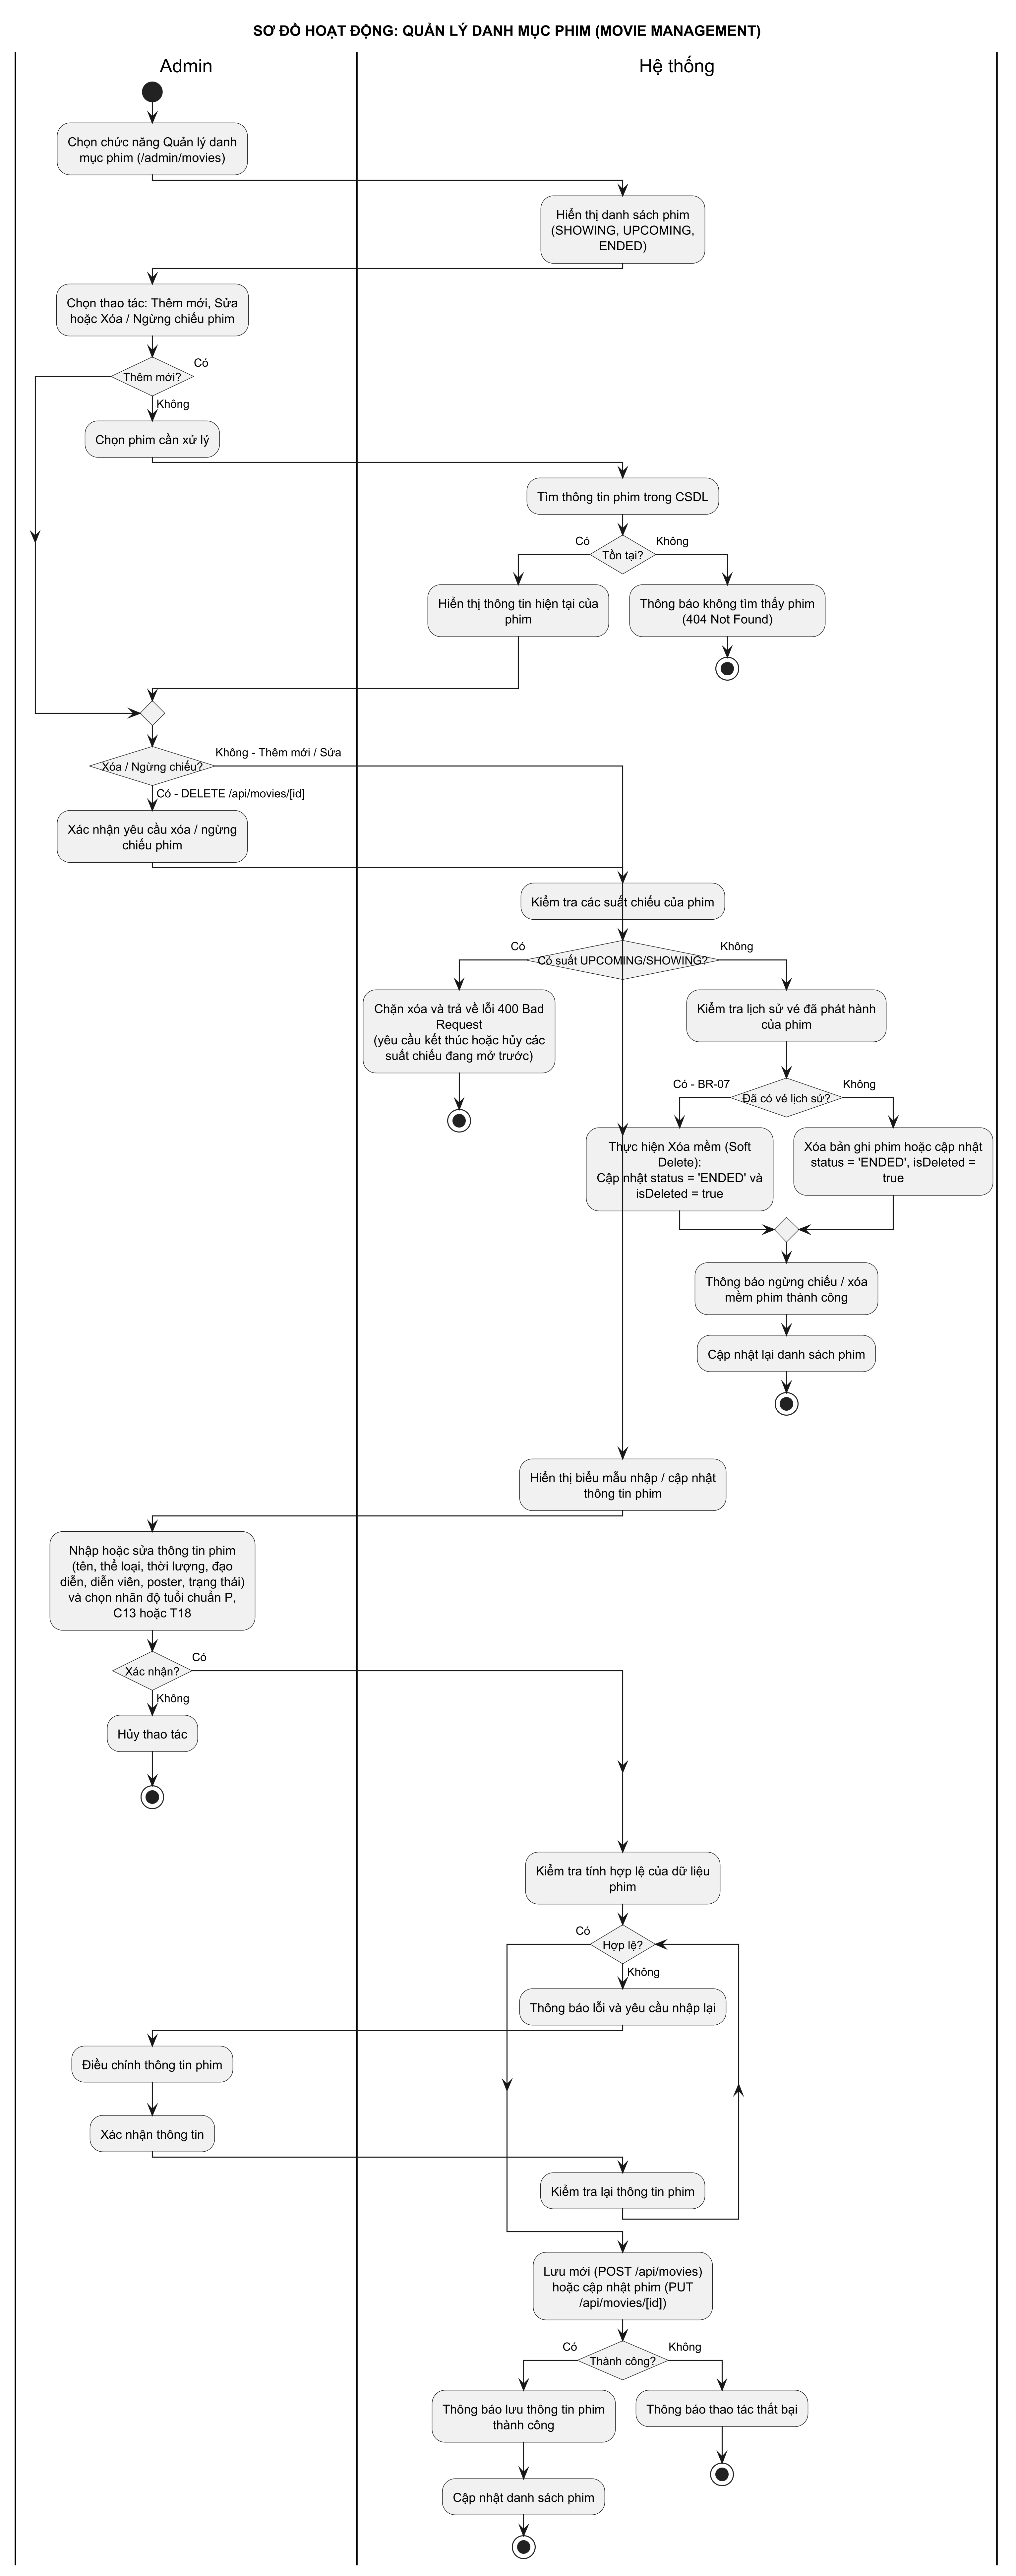
\includegraphics[width=\textwidth,height=0.80\textheight,keepaspectratio]{images/activity/13_quan_ly_phim.png}
  \caption{Activity Diagram: SƠ ĐỒ HOẠT ĐỘNG: QUẢN LÝ DANH MỤC PHIM (MOVIE MANAGEMENT)}
  \label{fig:act_13}
\end{figure}

\subsection{SƠ ĐỒ HOẠT ĐỘNG: LÊN LỊCH VÀ QUẢN LÝ SUẤT CHIẾU (SCREENING MANAGEMENT)}
\begin{figure}[H]
  \centering
  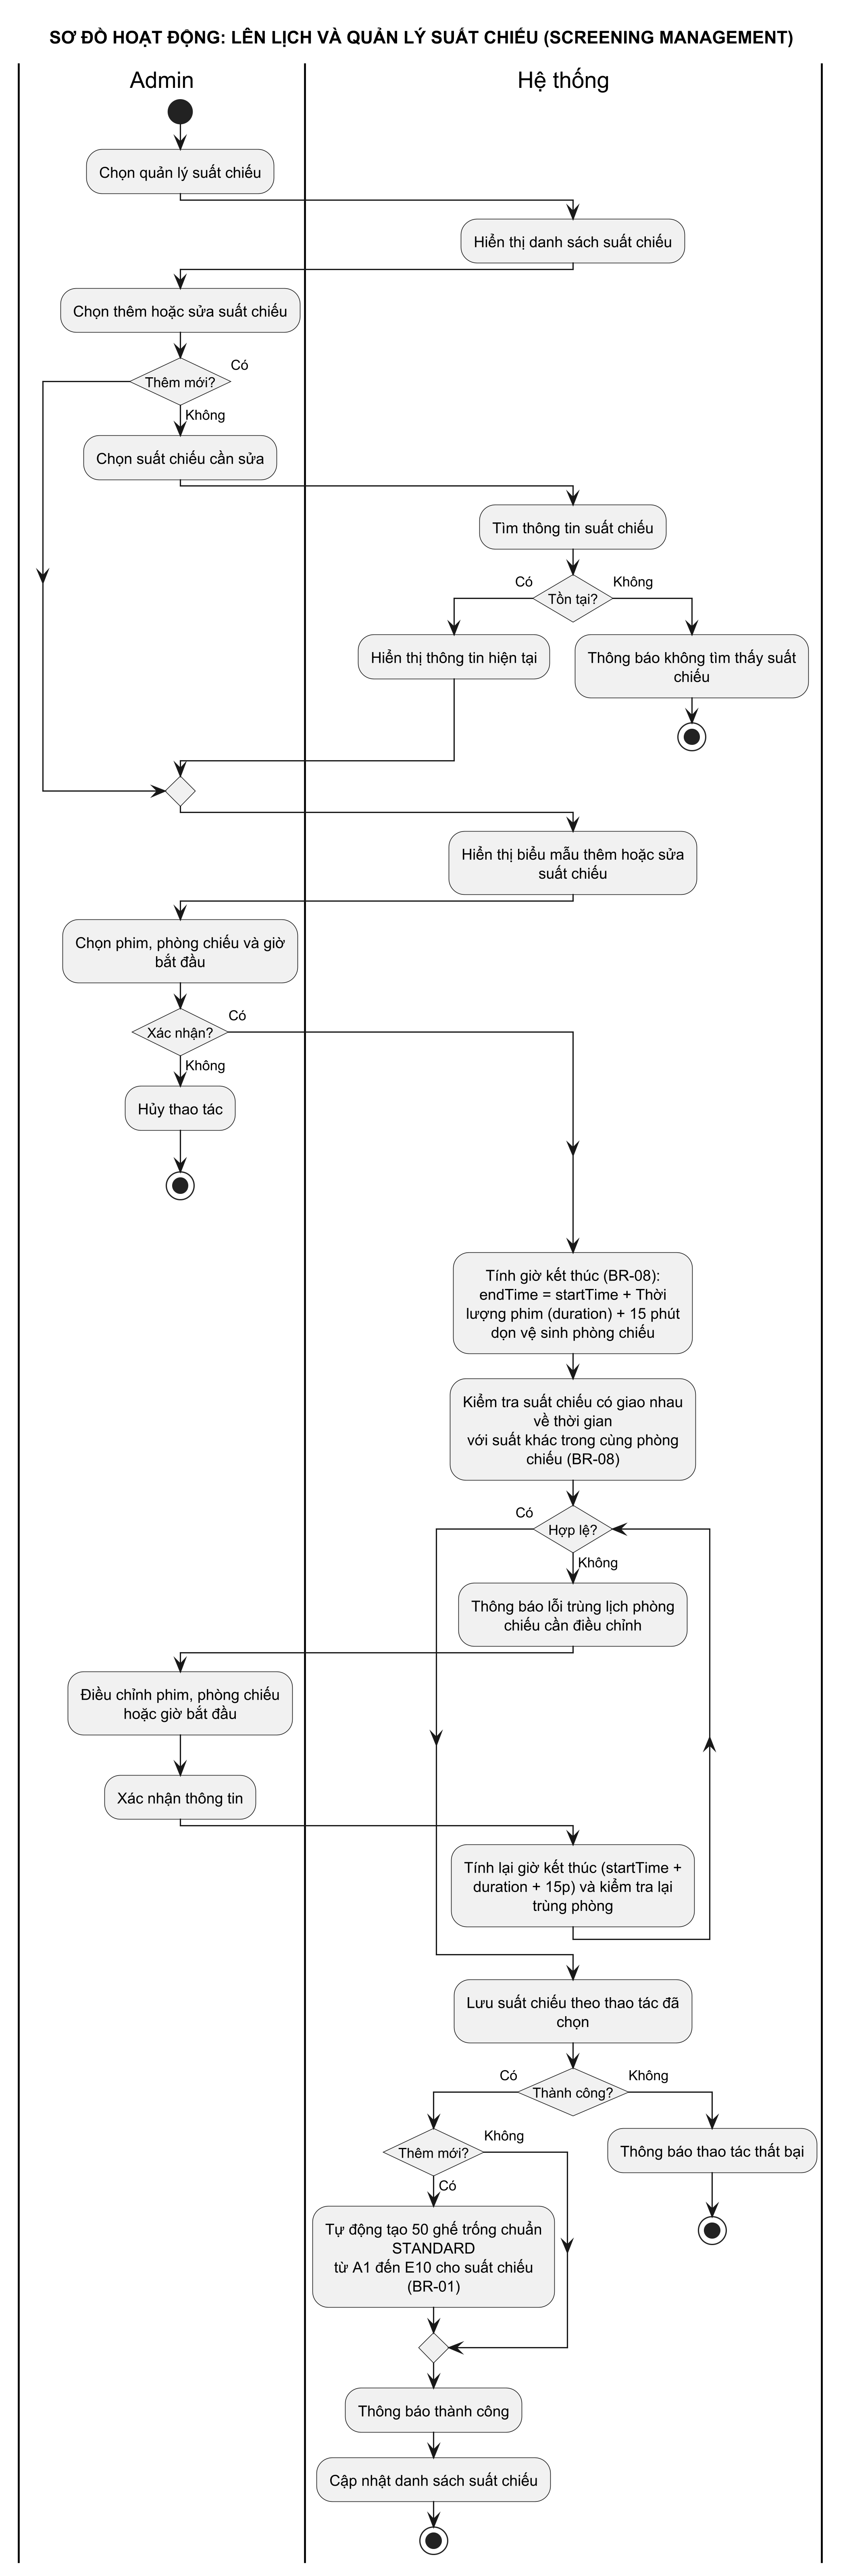
\includegraphics[width=\textwidth,height=0.80\textheight,keepaspectratio]{images/activity/14_quan_ly_suat_chieu.png}
  \caption{Activity Diagram: SƠ ĐỒ HOẠT ĐỘNG: LÊN LỊCH VÀ QUẢN LÝ SUẤT CHIẾU (SCREENING MANAGEMENT)}
  \label{fig:act_14}
\end{figure}

\subsection{SƠ ĐỒ HOẠT ĐỘNG: HỦY SUẤT CHIẾU KHẨN CẤP DO SỰ CỐ (DELETE /api/screenings/[id])}
\begin{figure}[H]
  \centering
  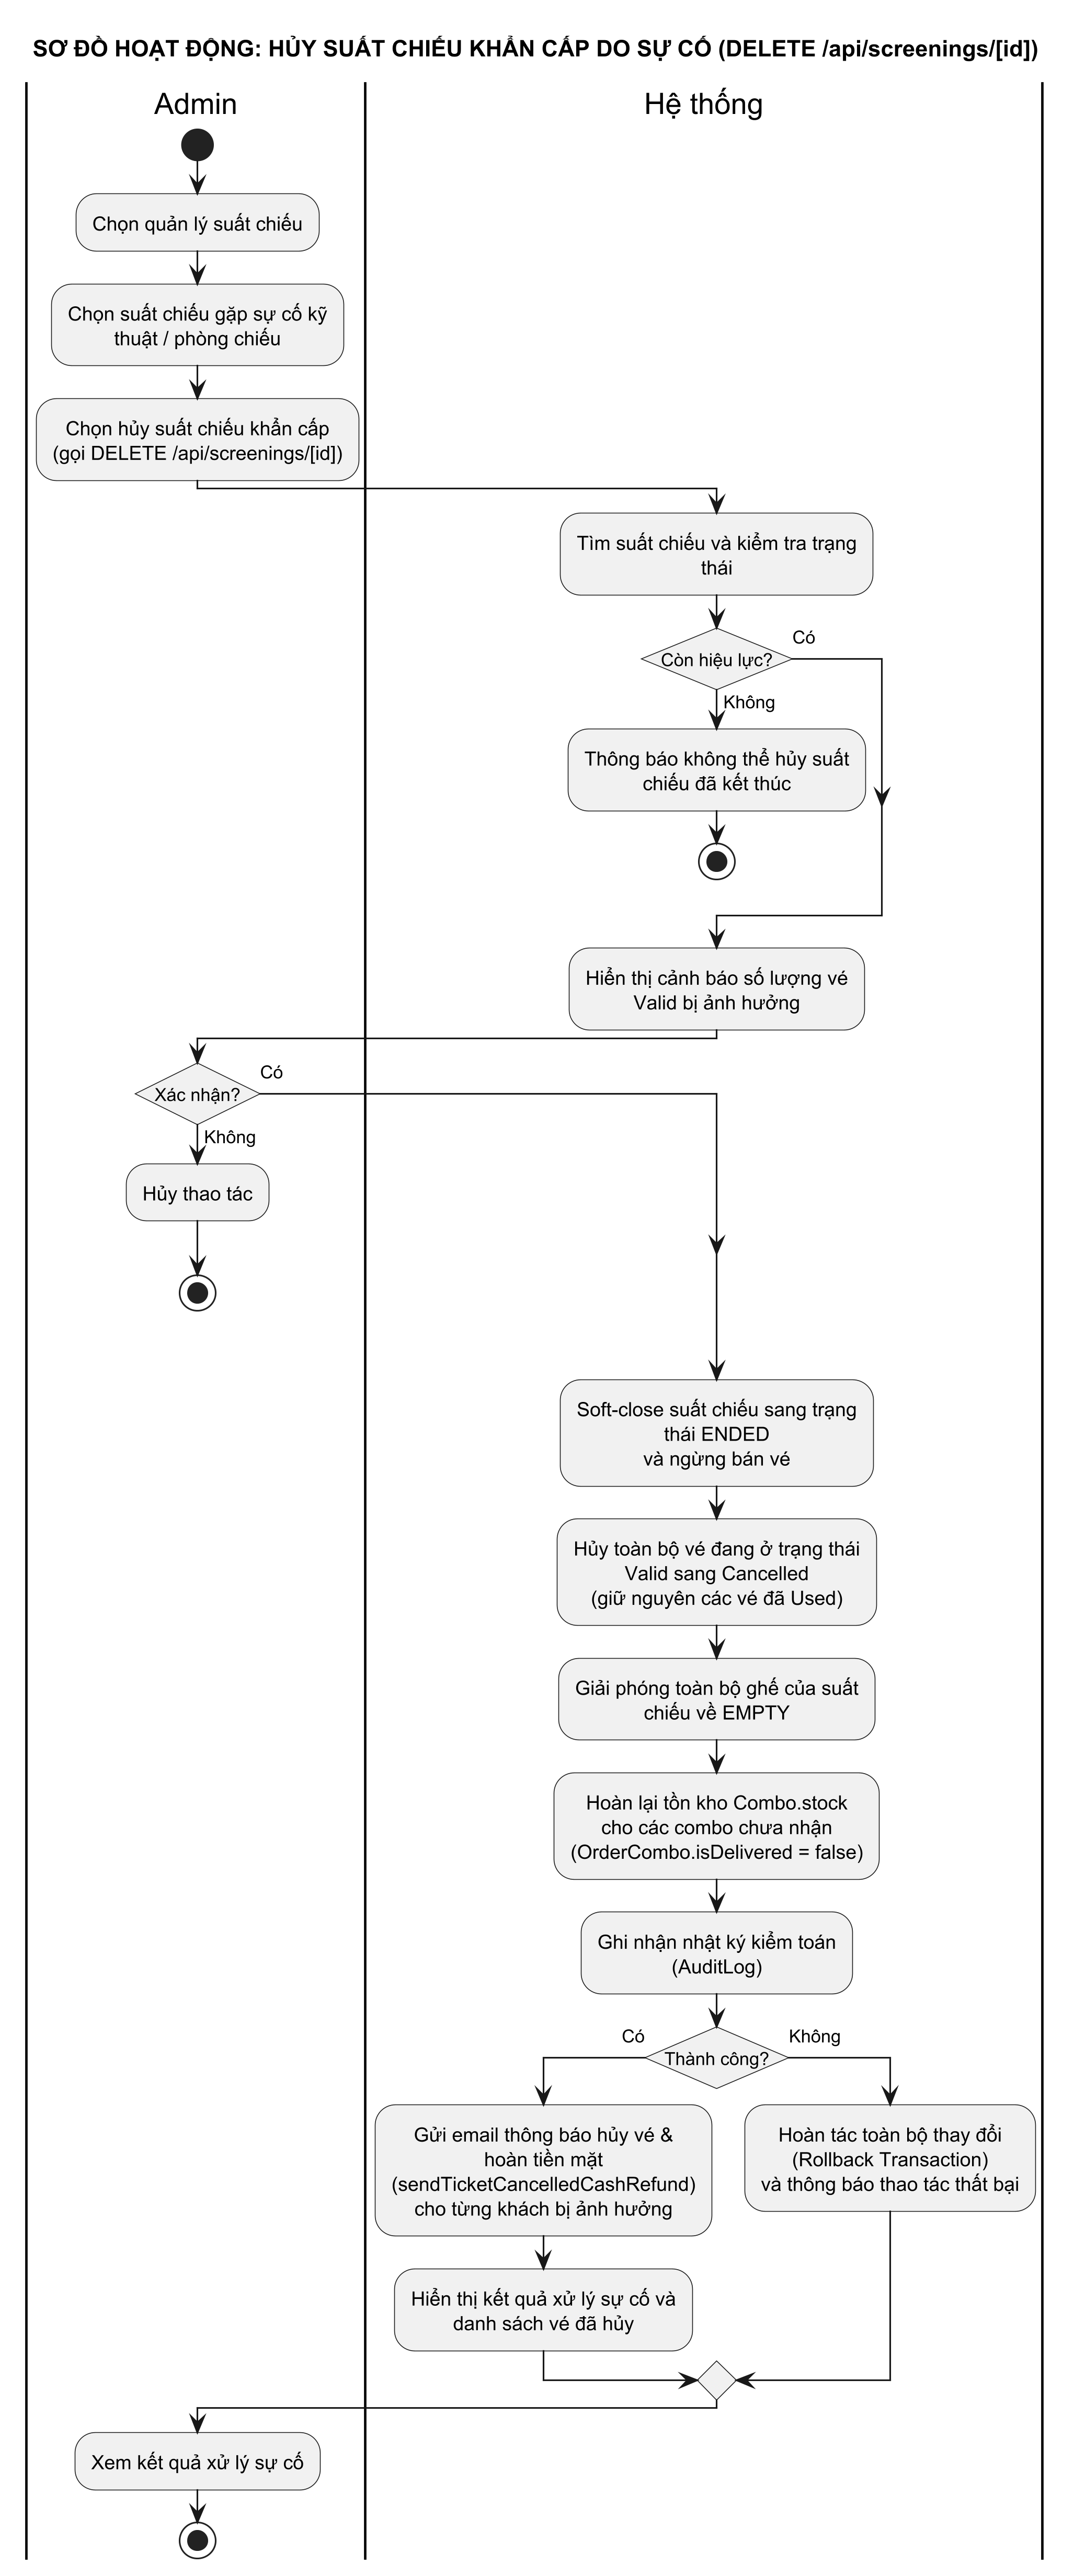
\includegraphics[width=\textwidth,height=0.80\textheight,keepaspectratio]{images/activity/15_huy_suat_chieu_khan_cap.png}
  \caption{Activity Diagram: SƠ ĐỒ HOẠT ĐỘNG: HỦY SUẤT CHIẾU KHẨN CẤP DO SỰ CỐ (DELETE /api/screenings/[id])}
  \label{fig:act_15}
\end{figure}

\subsection{SƠ ĐỒ HOẠT ĐỘNG: QUẢN LÝ COMBO BẮP NƯỚC (COMBO MANAGEMENT)}
\begin{figure}[H]
  \centering
  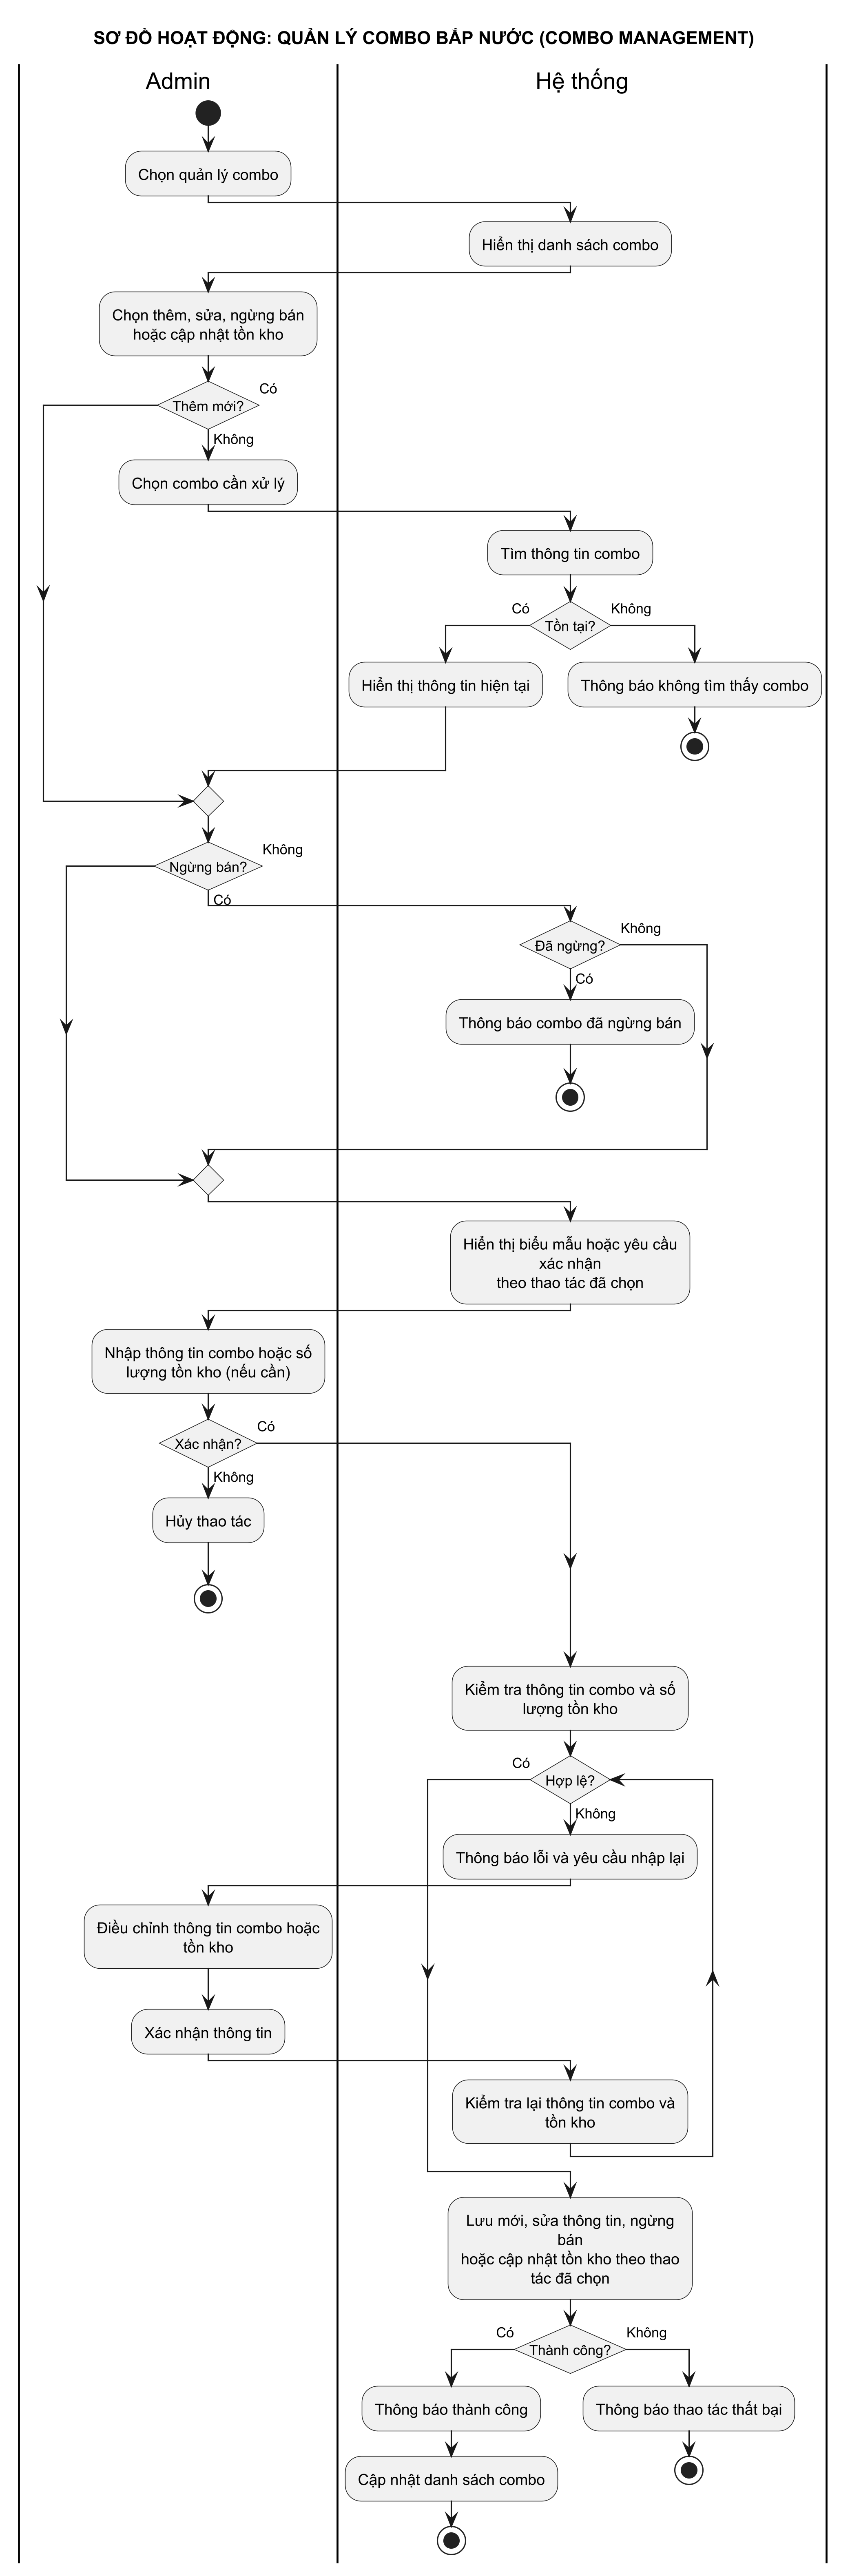
\includegraphics[width=\textwidth,height=0.80\textheight,keepaspectratio]{images/activity/16_quan_ly_combo.png}
  \caption{Activity Diagram: SƠ ĐỒ HOẠT ĐỘNG: QUẢN LÝ COMBO BẮP NƯỚC (COMBO MANAGEMENT)}
  \label{fig:act_16}
\end{figure}

\subsection{SƠ ĐỒ HOẠT ĐỘNG: DASHBOARD \& BÁO CÁO DOANH THU TÀI CHÍNH (ADMIN DASHBOARD \& REPORTS)}
\begin{figure}[H]
  \centering
  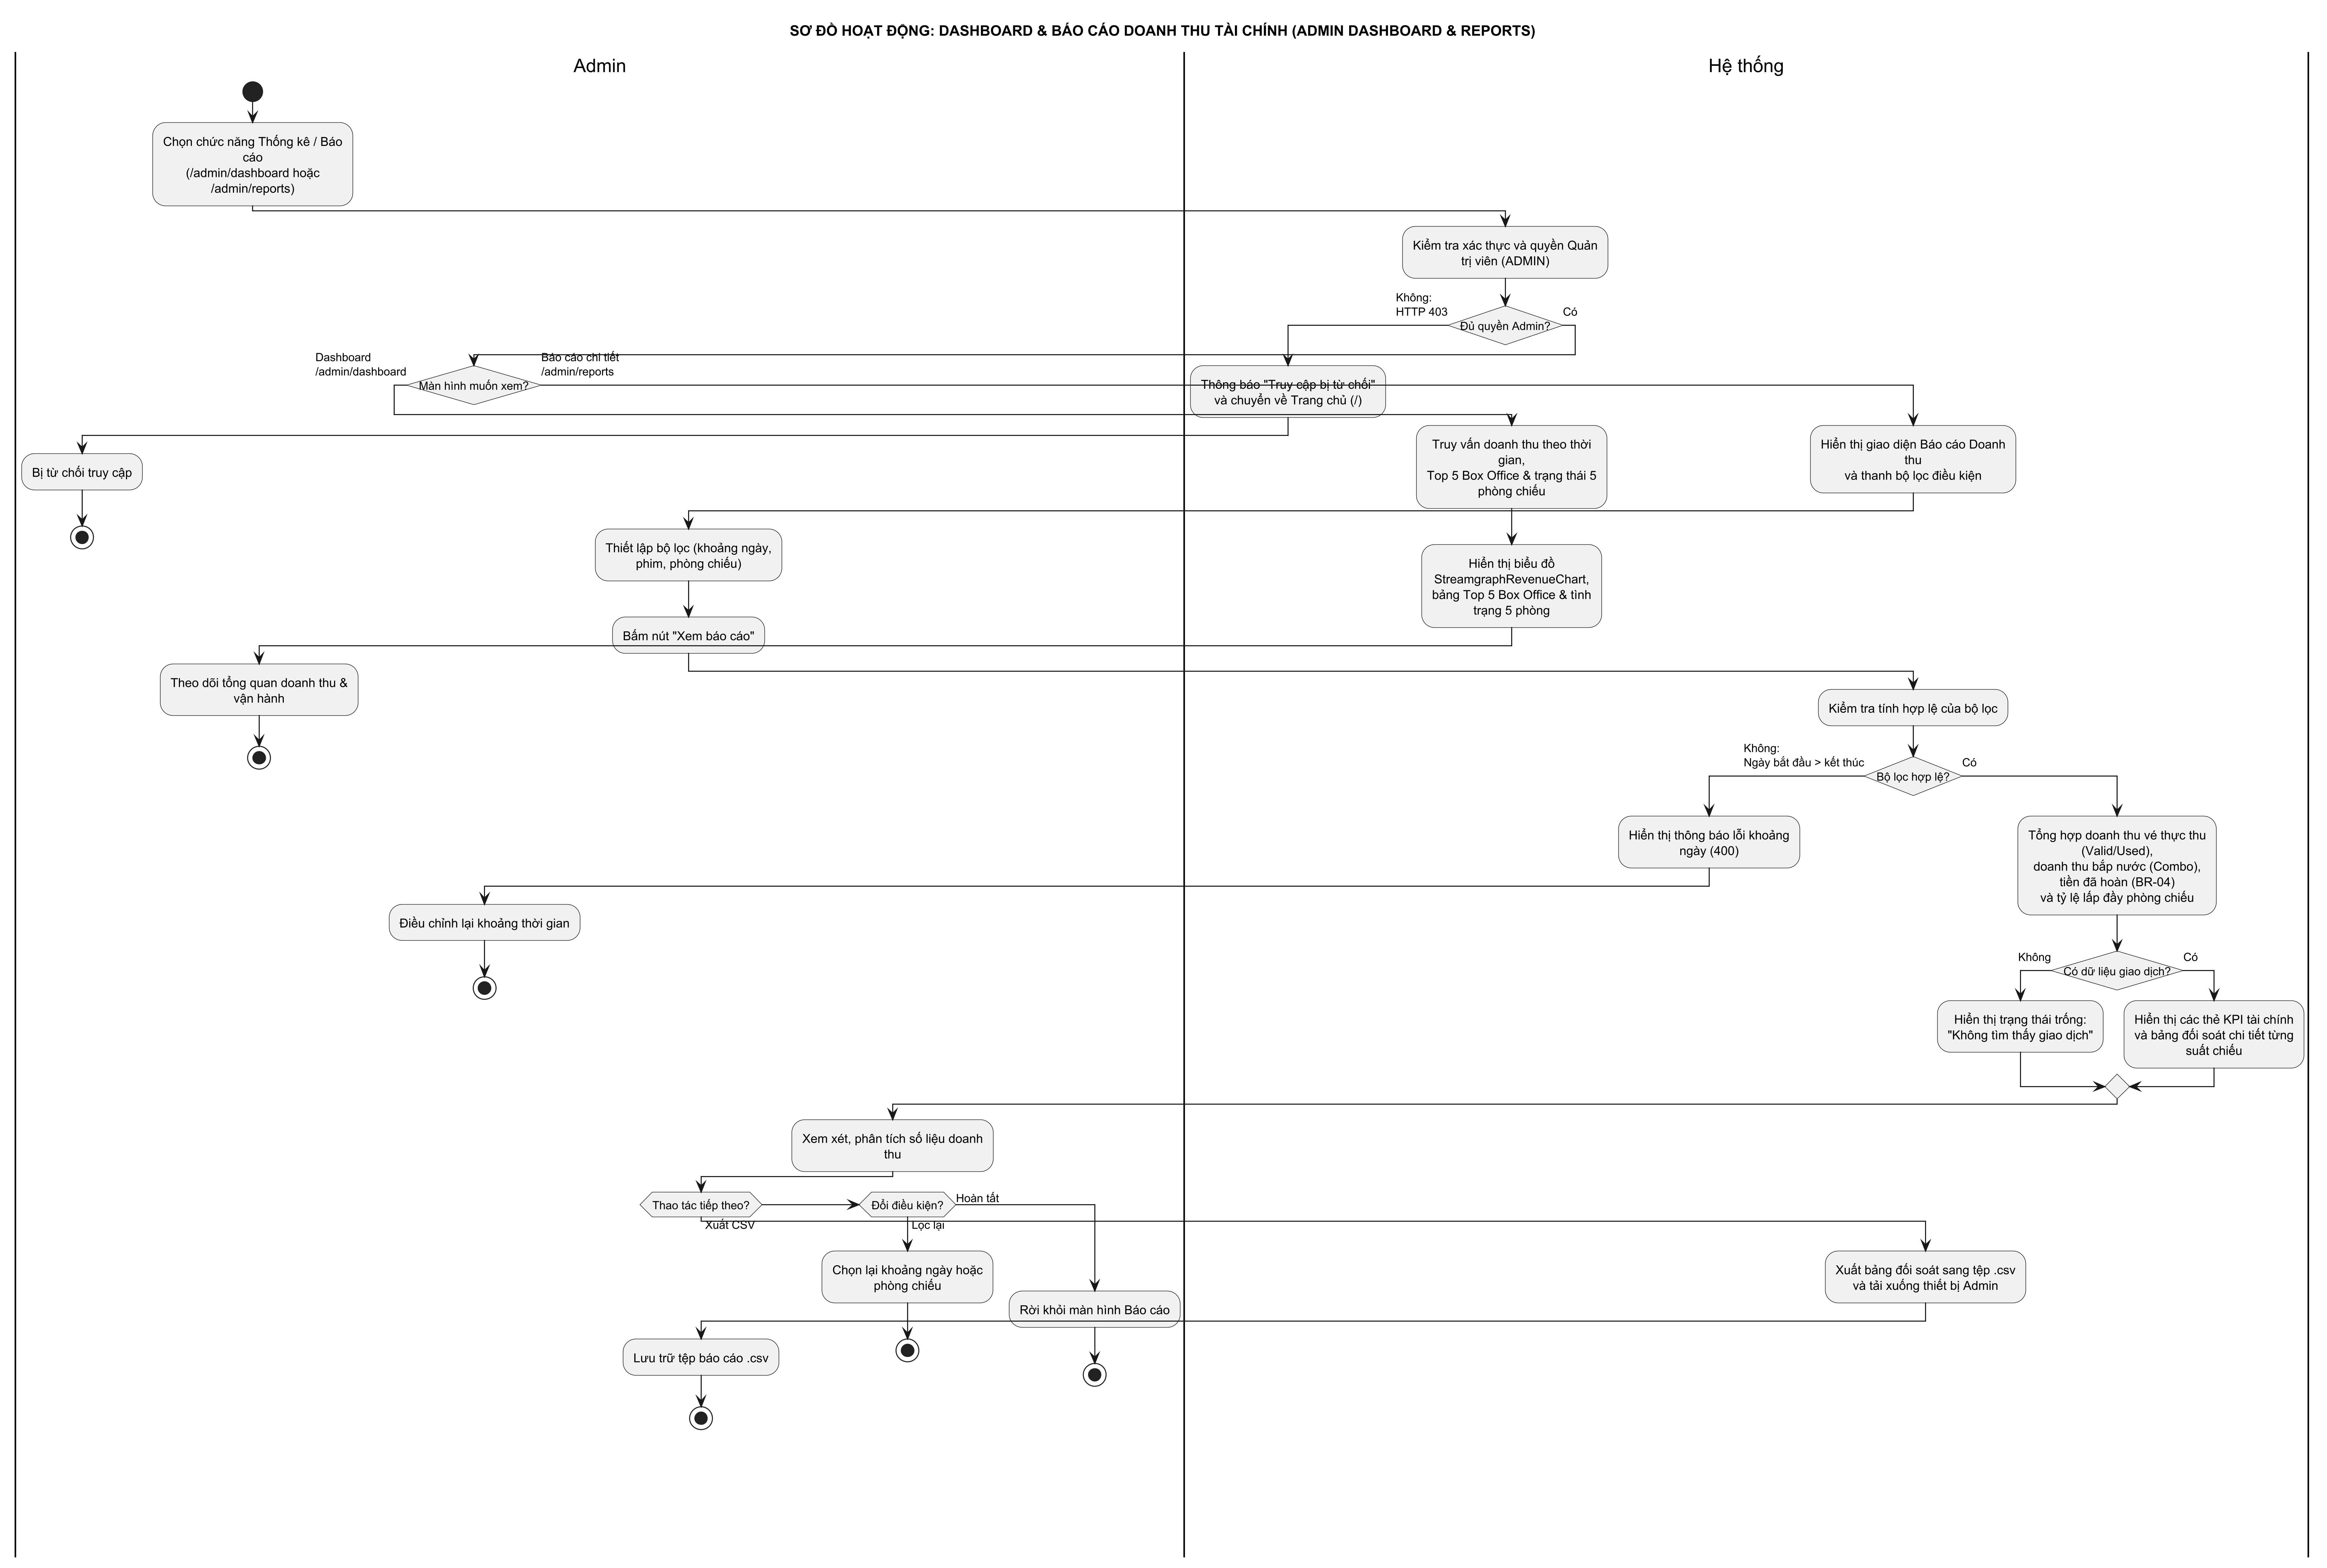
\includegraphics[width=\textwidth,height=0.80\textheight,keepaspectratio]{images/activity/17_bao_cao_doanh_thu.png}
  \caption{Activity Diagram: SƠ ĐỒ HOẠT ĐỘNG: DASHBOARD \& BÁO CÁO DOANH THU TÀI CHÍNH (ADMIN DASHBOARD \& REPORTS)}
  \label{fig:act_17}
\end{figure}


\section{Sơ đồ trạng thái (State Diagram)}
Phần này mô tả vòng đời và các bước chuyển trạng thái hợp lệ của 6 thực thể cốt lõi trong hệ thống: Vé (Ticket), Ghế suất chiếu (ShowtimeSeat), Thanh toán (Payment), Phim (Movie), Combo và Voucher.

\subsection{SƠ ĐỒ TRẠNG THÁI ĐƠN BẮP NƯỚC}
\begin{figure}[H]
  \centering
  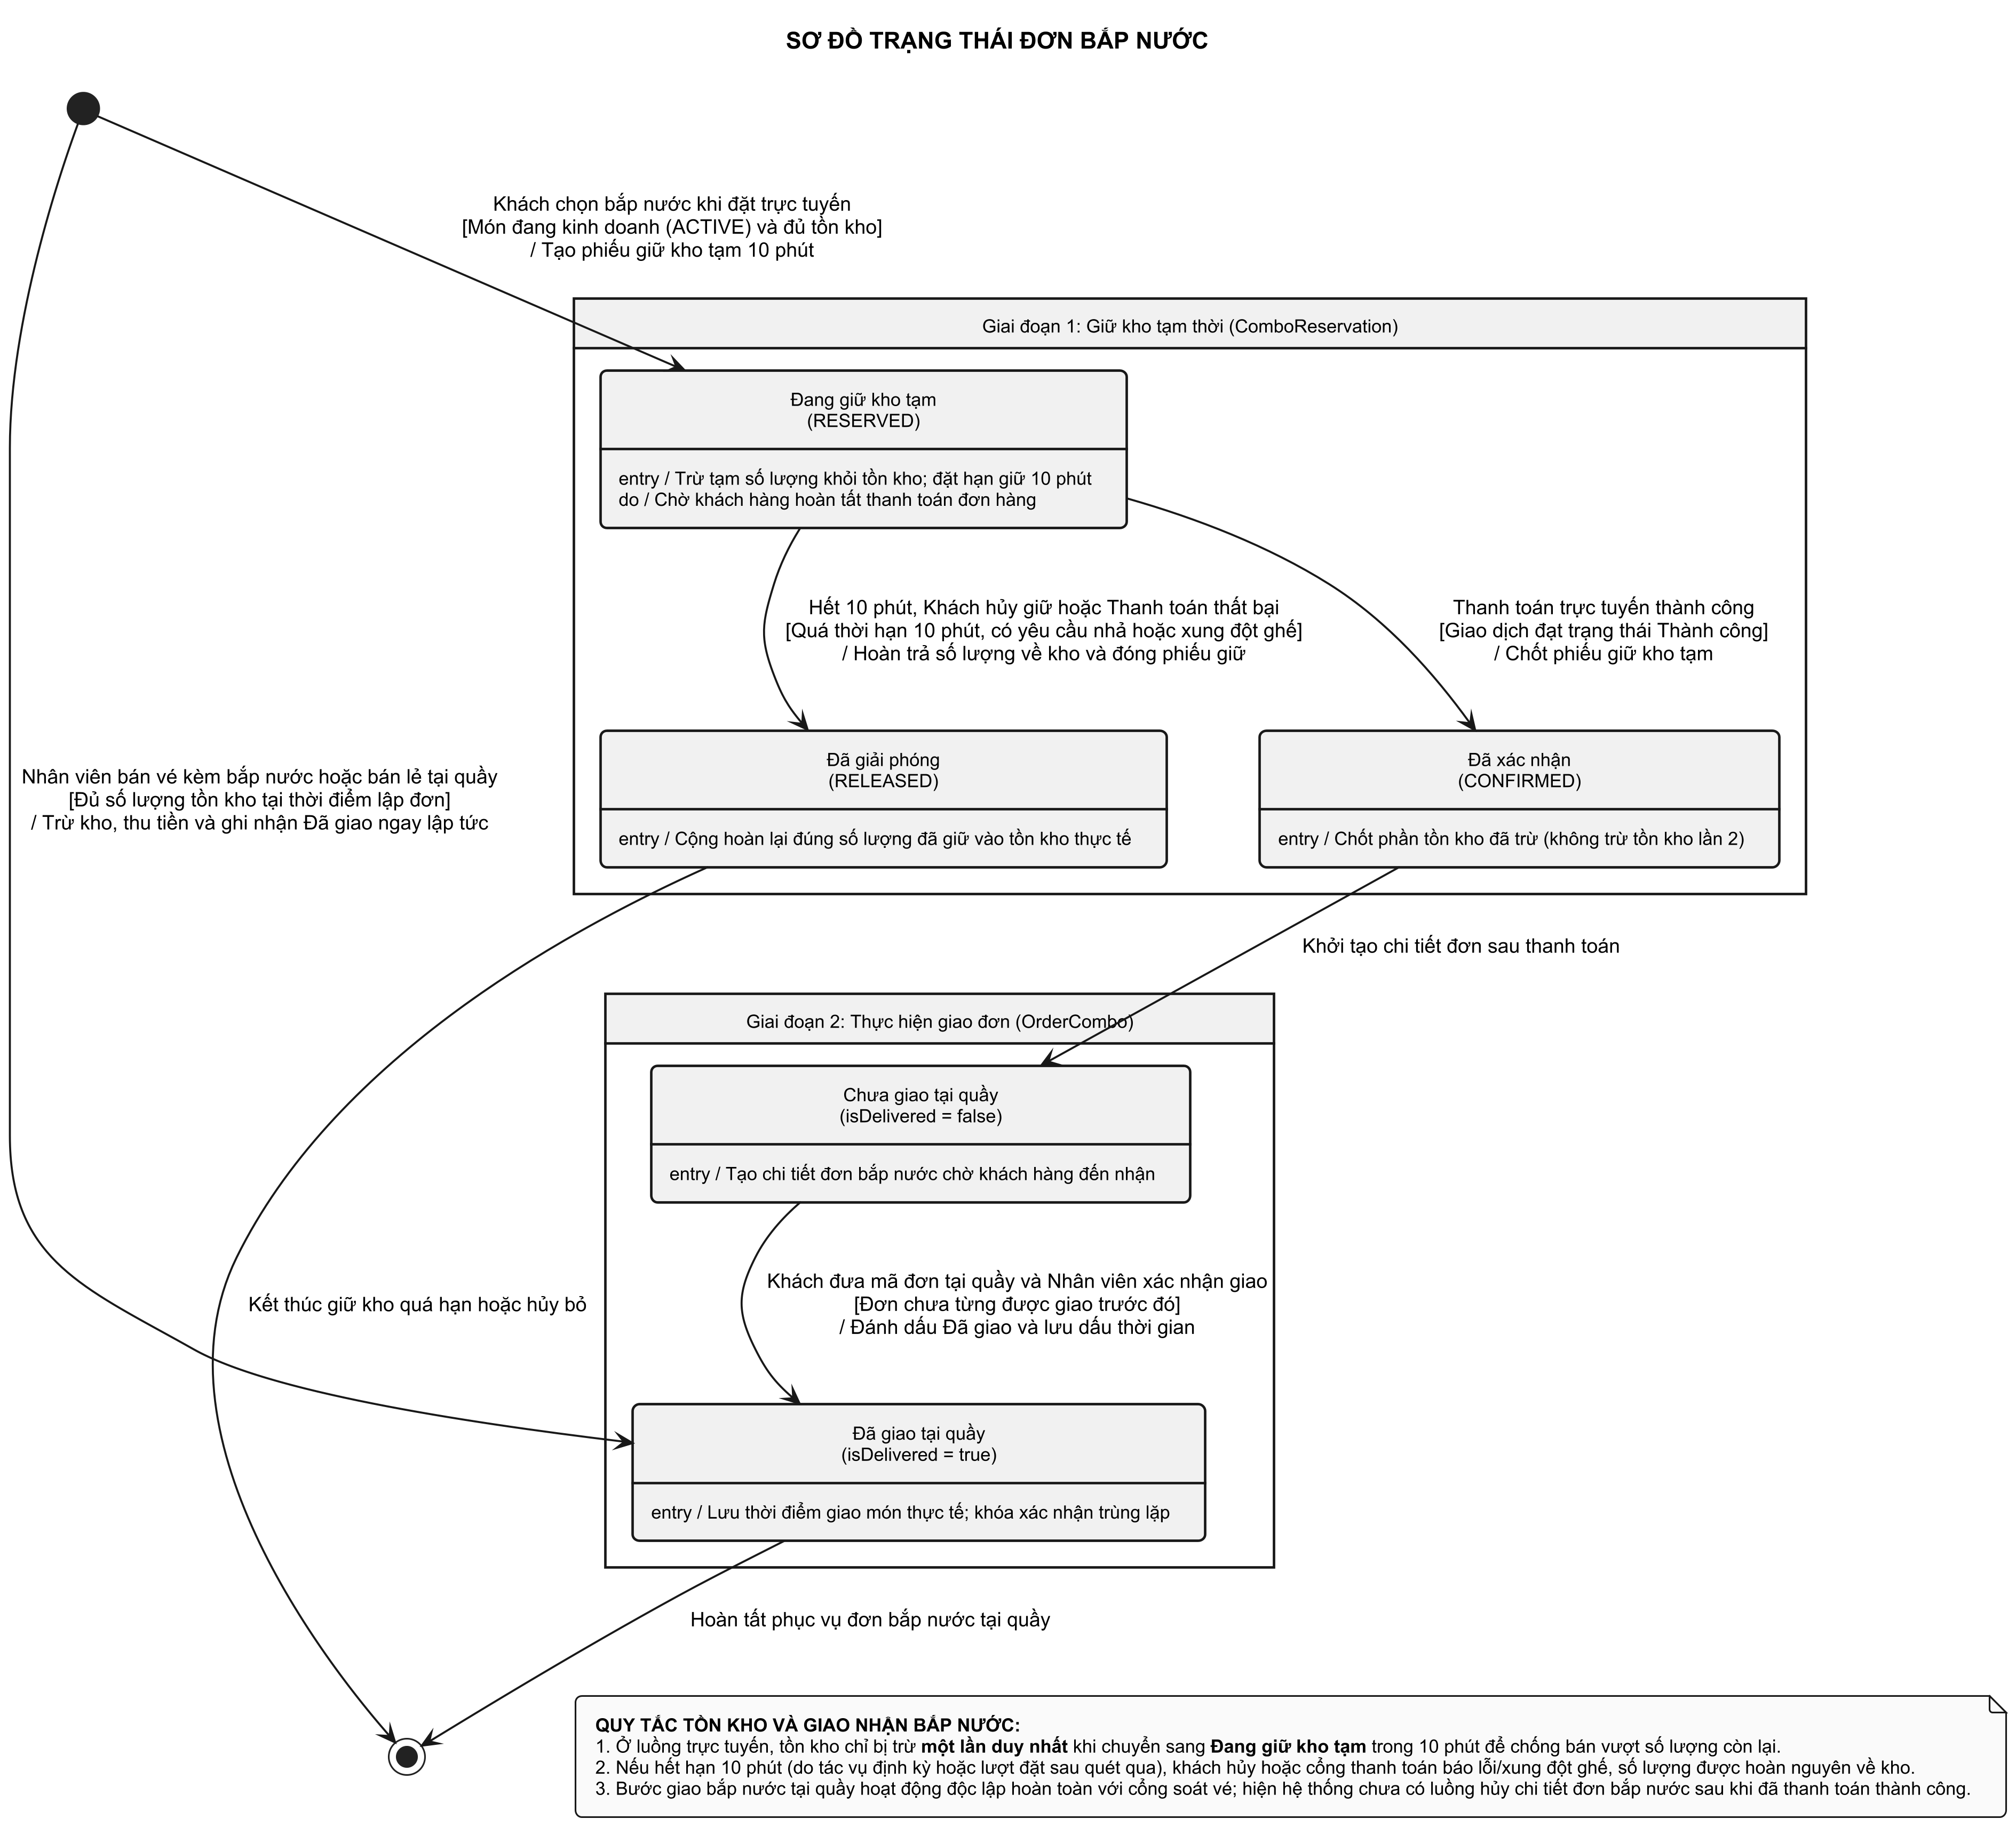
\includegraphics[width=\textwidth,height=0.80\textheight,keepaspectratio]{images/state/state_combo.png}
  \caption{State Diagram: SƠ ĐỒ TRẠNG THÁI ĐƠN BẮP NƯỚC}
  \label{fig:state_01}
\end{figure}

\subsection{SƠ ĐỒ TRẠNG THÁI VÒNG ĐỜI PHIM}
\begin{figure}[H]
  \centering
  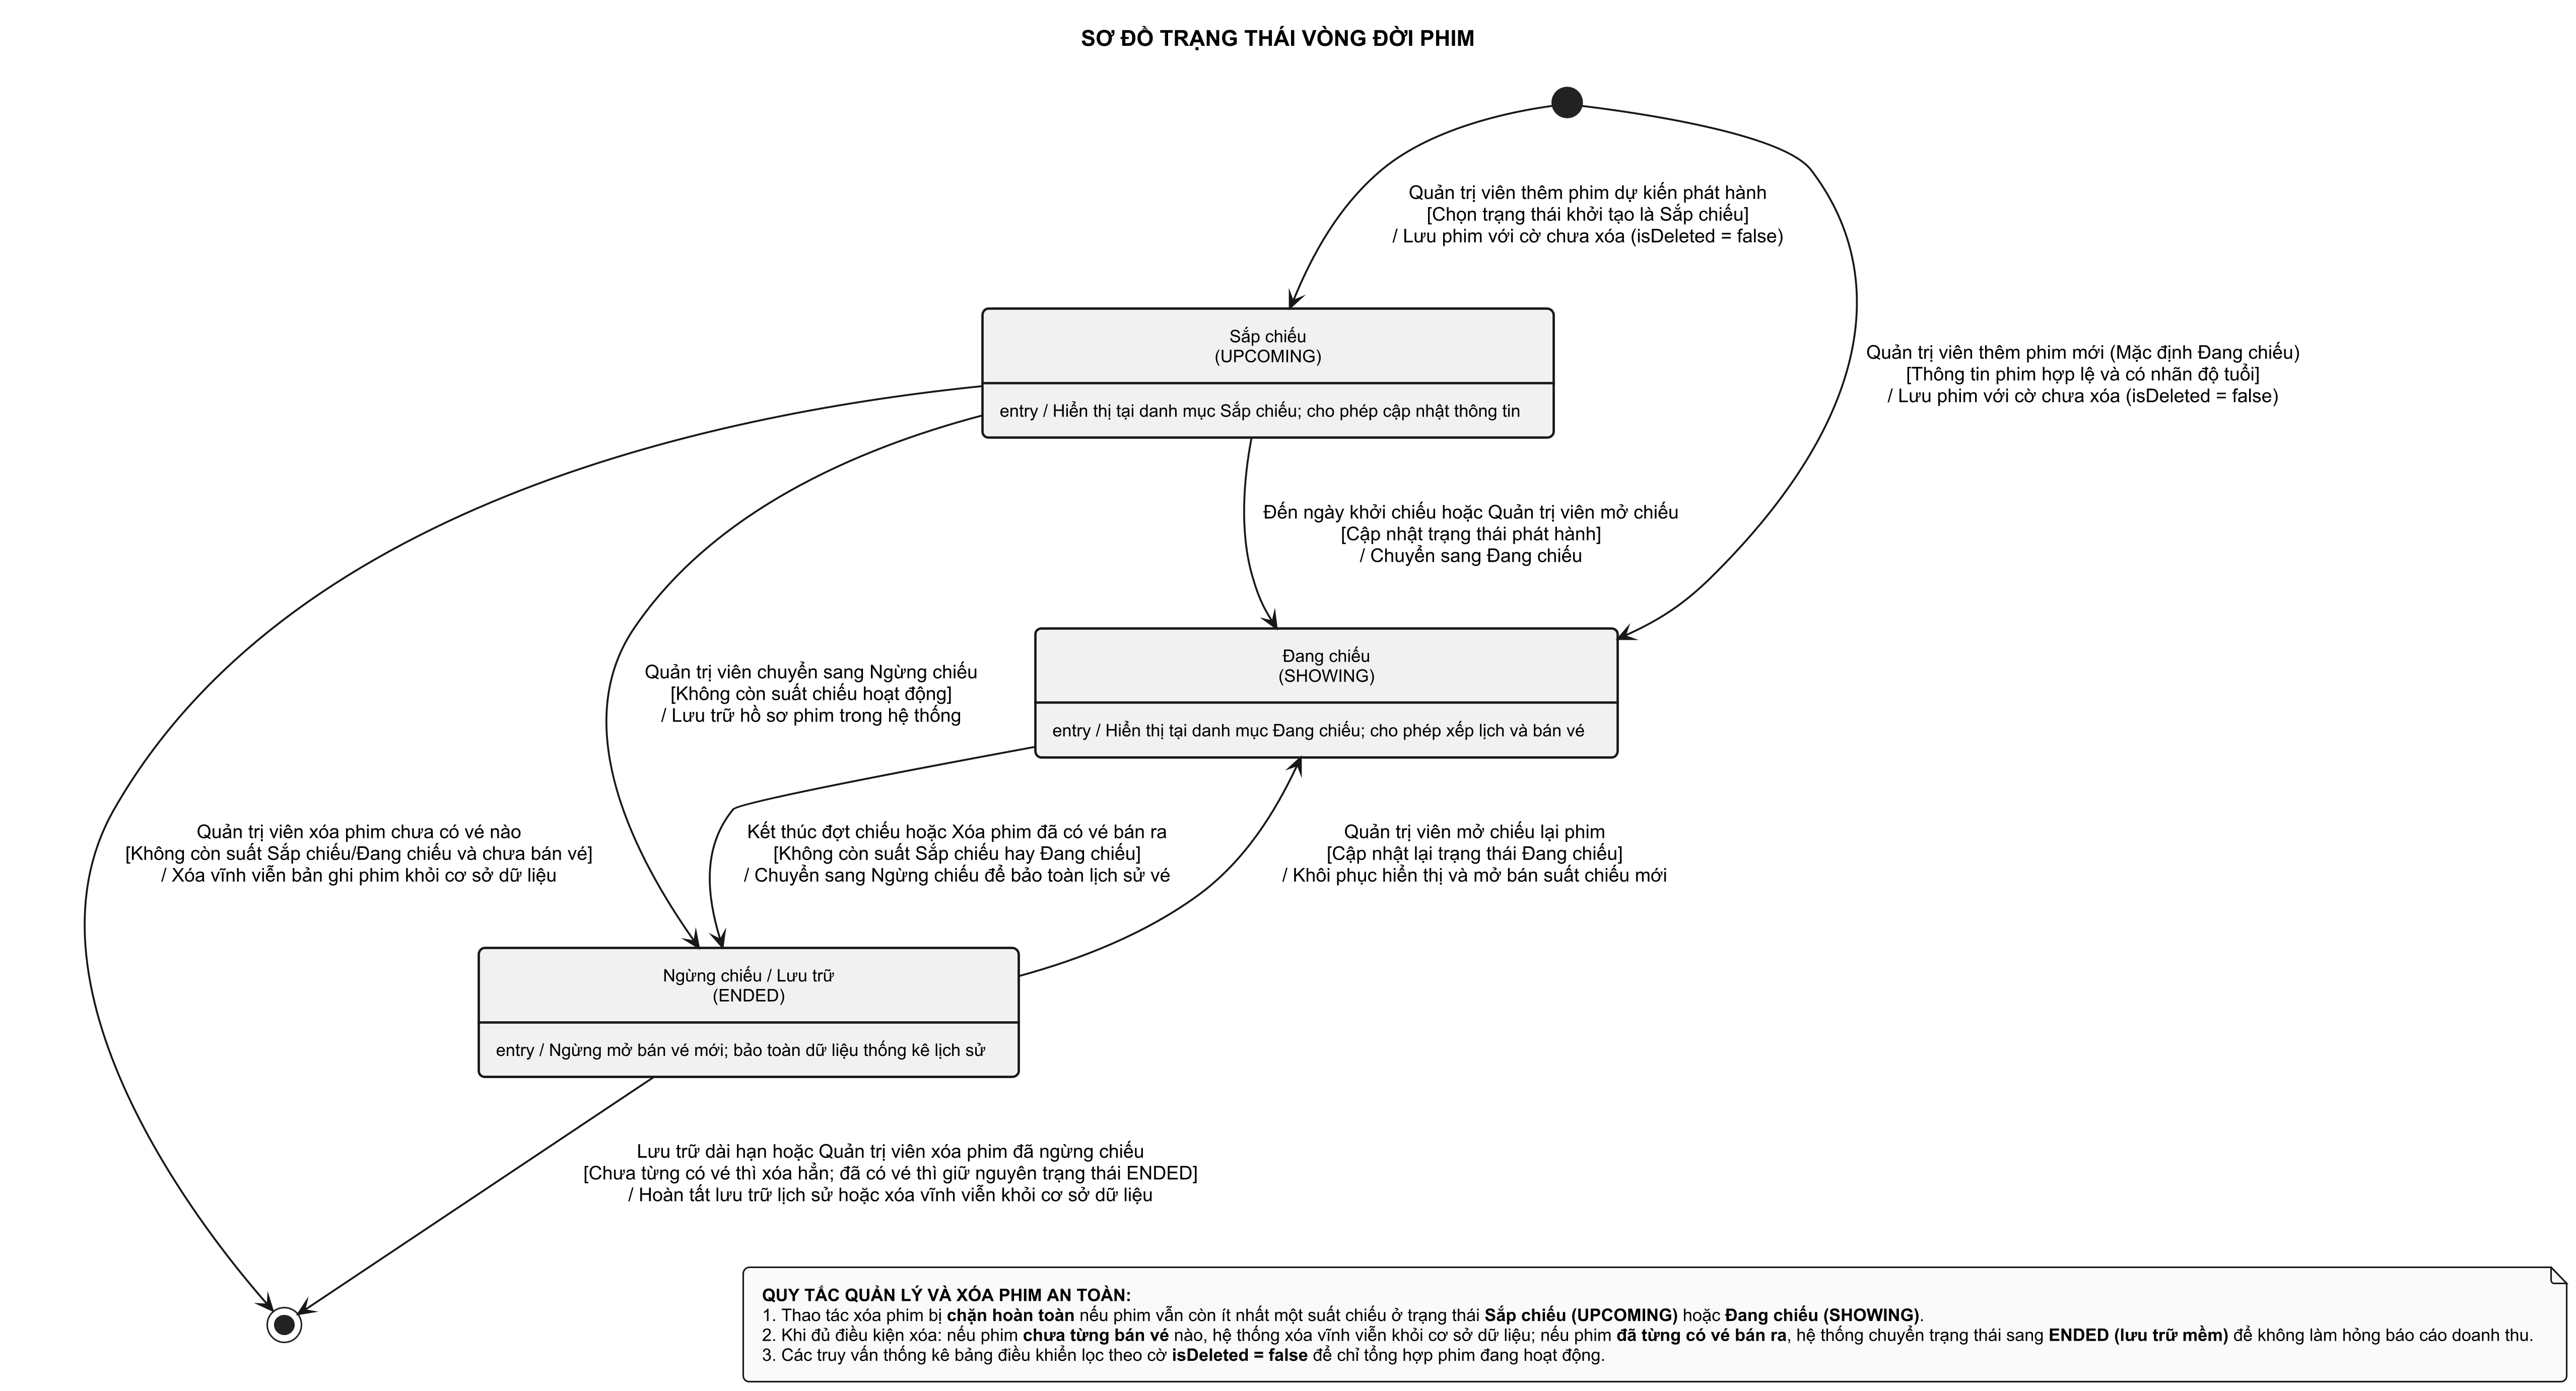
\includegraphics[width=\textwidth,height=0.80\textheight,keepaspectratio]{images/state/state_movie.png}
  \caption{State Diagram: SƠ ĐỒ TRẠNG THÁI VÒNG ĐỜI PHIM}
  \label{fig:state_02}
\end{figure}

\subsection{SƠ ĐỒ TRẠNG THÁI GIAO DỊCH THANH TOÁN}
\begin{figure}[H]
  \centering
  
\includegraphics[width=\textwidth,height=0.80\textheight,keepaspectratio]{images/state/state_payment.png}
  \caption{State Diagram: SƠ ĐỒ TRẠNG THÁI GIAO DỊCH THANH TOÁN}
  \label{fig:state_03}
\end{figure}

\subsection{SƠ ĐỒ TRẠNG THÁI SUẤT CHIẾU}
\begin{figure}[H]
  \centering
  
\includegraphics[width=\textwidth,height=0.80\textheight,keepaspectratio]{images/state/state_screening.png}
  \caption{State Diagram: SƠ ĐỒ TRẠNG THÁI SUẤT CHIẾU}
  \label{fig:state_04}
\end{figure}

\subsection{SƠ ĐỒ TRẠNG THÁI GHẾ THEO SUẤT CHIẾU}
\begin{figure}[H]
  \centering
  
\includegraphics[width=\textwidth,height=0.80\textheight,keepaspectratio]{images/state/state_seat.png}
  \caption{State Diagram: SƠ ĐỒ TRẠNG THÁI GHẾ THEO SUẤT CHIẾU}
  \label{fig:state_05}
\end{figure}

\subsection{SƠ ĐỒ TRẠNG THÁI VÉ XEM PHIM}
\begin{figure}[H]
  \centering
  
\includegraphics[width=\textwidth,height=0.80\textheight,keepaspectratio]{images/state/state_ticket.png}
  \caption{State Diagram: SƠ ĐỒ TRẠNG THÁI VÉ XEM PHIM}
  \label{fig:state_06}
\end{figure}


\section{Thiết kế lớp đối tượng (Class Diagram)}
\subsection{Sơ đồ lớp tổng thể}
Sơ đồ lớp đối tượng dưới đây thể hiện toàn bộ các thực thể nghiệp vụ, thuộc tính, phương thức và mối quan hệ giữa chúng trong hệ thống LumiCinema.

\begin{figure}[H]
  \centering
  \includegraphics[width=\textwidth,height=0.80\textheight,keepaspectratio]{images/class/class_diagram_lumicinema.png}
  \caption{Sơ đồ lớp đối tượng (Class Diagram) hệ thống LumiCinema}
  \label{fig:class_main}
\end{figure}

\subsection{Danh sách các lớp và mô tả chi tiết}
\begin{longtable}{|p{3.2cm}|p{6.2cm}|p{6.1cm}|}
\hline
\rowcolor{headerblue} \textbf{Tên lớp} & \textbf{Thuộc tính chính} & \textbf{Phương thức chính} \\ \hline
\endhead
\textbf{User} & \texttt{\small - id: Int; - email: String; - password: String; - name: String; - phone: String; - role: Role; - createdAt: DateTime} & \texttt{\small + register(email: String, password: String, name: String, phone: String): Boolean; + login(email: String, password: String): String; + updateProfile(name: String, phone: String): Boolean; + changePassword(oldPass: String, newPass: String): Boolean} \\ \hline
\textbf{Customer} & \texttt{\small } & \texttt{\small + bookTicket(screeningId: Int, seatIds: List<Int>, couponCode: String): Payment; + selectCombo(comboId: Int, quantity: Int): Void; + applyCoupon(code: String): Decimal; + cancelTicket(ticketId: Int, reason: String): Boolean; + writeReview(movieId: Int, rating: Int, comment: String): Review} \\ \hline
\textbf{Staff} & \texttt{\small } & \texttt{\small + sellTicketAtPOS(screeningId: Int, seatIds: List<Int>, method: PaymentMethod): Payment; + sellComboAtPOS(comboId: Int, quantity: Int, method: PaymentMethod): Payment; + checkInTicket(ticketCode: String): Boolean; + deliverCombo(orderComboId: Int): Void} \\ \hline
\textbf{Admin} & \texttt{\small } & \texttt{\small + createMovie(movieData: Movie): Movie; + scheduleScreening(screeningData: Screening): Screening; + manageCombo(comboData: Combo): Combo; + issueCoupon(couponData: Coupon): Coupon; + viewReports(from: Date, to: Date): ReportData} \\ \hline
\textbf{Movie} & \texttt{\small - id: Int; - title: String; - slug: String; - description: String; - duration: Int; - releaseDate: Date; - endDate: Date; - ageRating: String; - poster: String; - trailer: String; - genre: String; - director: String ...} & \texttt{\small + getActiveScreenings(): List<Screening>; + calculateAverageRating(): Decimal; + updateStatus(newStatus: MovieStatus): Void; + softDelete(): Void} \\ \hline
\textbf{Screening} & \texttt{\small - id: Int; - room: String; - roomNumber: Int; - startTime: DateTime; - endTime: DateTime; - date: Date; - price: Decimal; - status: ScreeningStatus} & \texttt{\small + checkRoomConflict(startTime: DateTime, endTime: DateTime, roomNumber: Int): Boolean; + generateSeats(): Void; + cancelScreening(reason: String): Boolean} \\ \hline
\textbf{Seat} & \texttt{\small - id: Int; - room: String; - row: String; - number: Int; - code: String; - type: SeatType; - status: SeatStatus; - reservedUntil: DateTime} & \texttt{\small + holdSeat(durationMinutes: Int): Boolean; + releaseSeat(): Void; + markAsOccupied(): Void} \\ \hline
\textbf{Pricing} & \texttt{\small - id: Int; - ticketType: String; - label: String; - percentage: Int; - basePrice: Decimal; - description: String} & \texttt{\small + calculateFinalPrice(basePrice: Decimal, seatType: SeatType): Decimal} \\ \hline
\textbf{Ticket} & \texttt{\small - id: Int; - ticketType: String; - price: Decimal; - purchaseDate: DateTime; - status: TicketStatus; - cancellationReason: String} & \texttt{\small + generateQRCode(): String; + checkIn(): Boolean; + cancelTicket(reason: String): Boolean; + cancelByCustomer(): Coupon; + cancelByIncident(reason: String): Void} \\ \hline
\textbf{Payment} & \texttt{\small - id: Int; - amount: Decimal; - paymentMethod: PaymentMethod; - transactionCode: String; - status: PaymentStatus; - screeningId: Int?; - seatIds: Json?; - couponCode: String?; - ticketItems: Json?; - createdAt: DateTime} & \texttt{\small + calculateTotal(tickets: List<Ticket>, combos: List<OrderCombo>, coupon: Coupon): Decimal; + createPaymentUrl(gateway: PaymentMethod): String; + processIPNCallback(data: Map<String, String>): Boolean; + issueRefund(amount: Decimal, method: PaymentMethod): Boolean} \\ \hline
\textbf{ThirdPartyAccount} & \texttt{\small - id: Int; - provider: String; - accountNumber: String; - accountName: String; - balance: Decimal; - updatedAt: DateTime} & \texttt{\small (Entity/DTO)} \\ \hline
\textbf{Coupon} & \texttt{\small - id: Int; - code: String; - discountType: DiscountType; - discountValue: Decimal; - minAmount: Decimal; - maxUsage: Int; - usedCount: Int; - expiryDate: Date} & \texttt{\small + validateCoupon(orderAmount: Decimal, movieId: Int): Boolean; + calculateDiscount(ticketAmount: Decimal): Decimal; + markAsUsed(): Void} \\ \hline
\textbf{Combo} & \texttt{\small - id: Int; - name: String; - description: String; - price: Decimal; - stock: Int; - status: ComboStatus; - image: String; - reservedUntil: DateTime} & \texttt{\small + checkStockAvailability(quantity: Int): Boolean; + deductStock(quantity: Int): Void; + restock(quantity: Int): Void} \\ \hline
\textbf{OrderCombo} & \texttt{\small - id: Int; - quantity: Int; - price: Decimal; - isDelivered: Boolean; - deliveredAt: DateTime} & \texttt{\small + markAsDelivered(): Void; + getSubtotal(): Decimal} \\ \hline
\textbf{ComboReservation} & \texttt{\small - id: Int; - quantity: Int; - status: String; - reservedUntil: DateTime} & \texttt{\small + checkExpiry(): Boolean; + release(): Void} \\ \hline
\textbf{Review} & \texttt{\small - id: Int; - rating: Int; - comment: String; - createdAt: DateTime} & \texttt{\small + createReview(userId: Int, movieId: Int, rating: Int, comment: String): Boolean; + hideReview(): Void} \\ \hline
\textbf{AuditLog} & \texttt{\small - id: Int; - actorId: Int; - action: String; - targetEntity: String; - targetId: Int; - metadata: String; - createdAt: DateTime} & \texttt{\small + recordLog(actorId: Int, action: String, targetEntity: String, targetId: Int, metadata: String): Void} \\ \hline
\textbf{ZaloPayService} & \texttt{\small - appId: String; - key1: String; - key2: String; - endpoint: String} & \texttt{\small + generateZaloPayTransId(): String; + calculateZaloPayOrderMac(data: String): String; + createZaloPayOrder(payment: Payment): ZaloOrderResponse; + verifyZaloPayCallback(data: String, receivedMac: String): Boolean} \\ \hline
\textbf{VNPayService} & \texttt{\small - tmnCode: String; - hashSecret: String; - paymentUrl: String} & \texttt{\small + signVnpayParams(params: Map<String, String>): String; + verifyVnpaySignature(queryParams: Map<String, String>): Boolean} \\ \hline
\textbf{ThirdPartyWalletService} & \texttt{\small } & \texttt{\small + getThirdPartyAccounts(provider: String): List<ThirdPartyAccount>; + topupThirdPartyAccount(accountId: Int, amount: Decimal): ThirdPartyAccount; + resetThirdPartyAccount(accountId: Int): ThirdPartyAccount; + debitThirdPartyAccountIfSufficient(accountId: Int, amount: Decimal): Boolean; + refundThirdPartyAccount(accountId: Int, amount: Decimal): ThirdPartyAccount} \\ \hline
\textbf{EmailService} & \texttt{\small } & \texttt{\small + sendTicketConfirmation(to: String, payment: Payment, tickets: List<Ticket>): Void; + sendVoucherIssued(to: String, coupon: Coupon): Void; + sendTicketCancelledCashRefund(to: String, ticket: Ticket, reason: String): Void} \\ \hline
\textbf{SeatExpirationService} & \texttt{\small - holdDurationMinutes: Int} & \texttt{\small + releaseExpiredSeatsAndCombos(screeningId: Int): Int; + reserveSeatsAtomic(screeningId: Int, seatIds: List<Int>): Boolean} \\ \hline
\end{longtable}

\section{Thiết kế Cơ sở dữ liệu (ERD \& RDM)}
Cơ sở dữ liệu hệ thống LumiCinema được thiết kế trên hệ quản trị PostgreSQL 16 (quản lý schema qua Prisma ORM), gồm \textbf{12 bảng}, \textbf{10 kiểu liệt kê (Enum)} và \textbf{15 khóa ngoại vật lý}.

\subsection{Sơ đồ thực thể kết hợp (ERD) và Mô hình dữ liệu quan hệ (RDM)}
\begin{figure}[H]
  \centering
  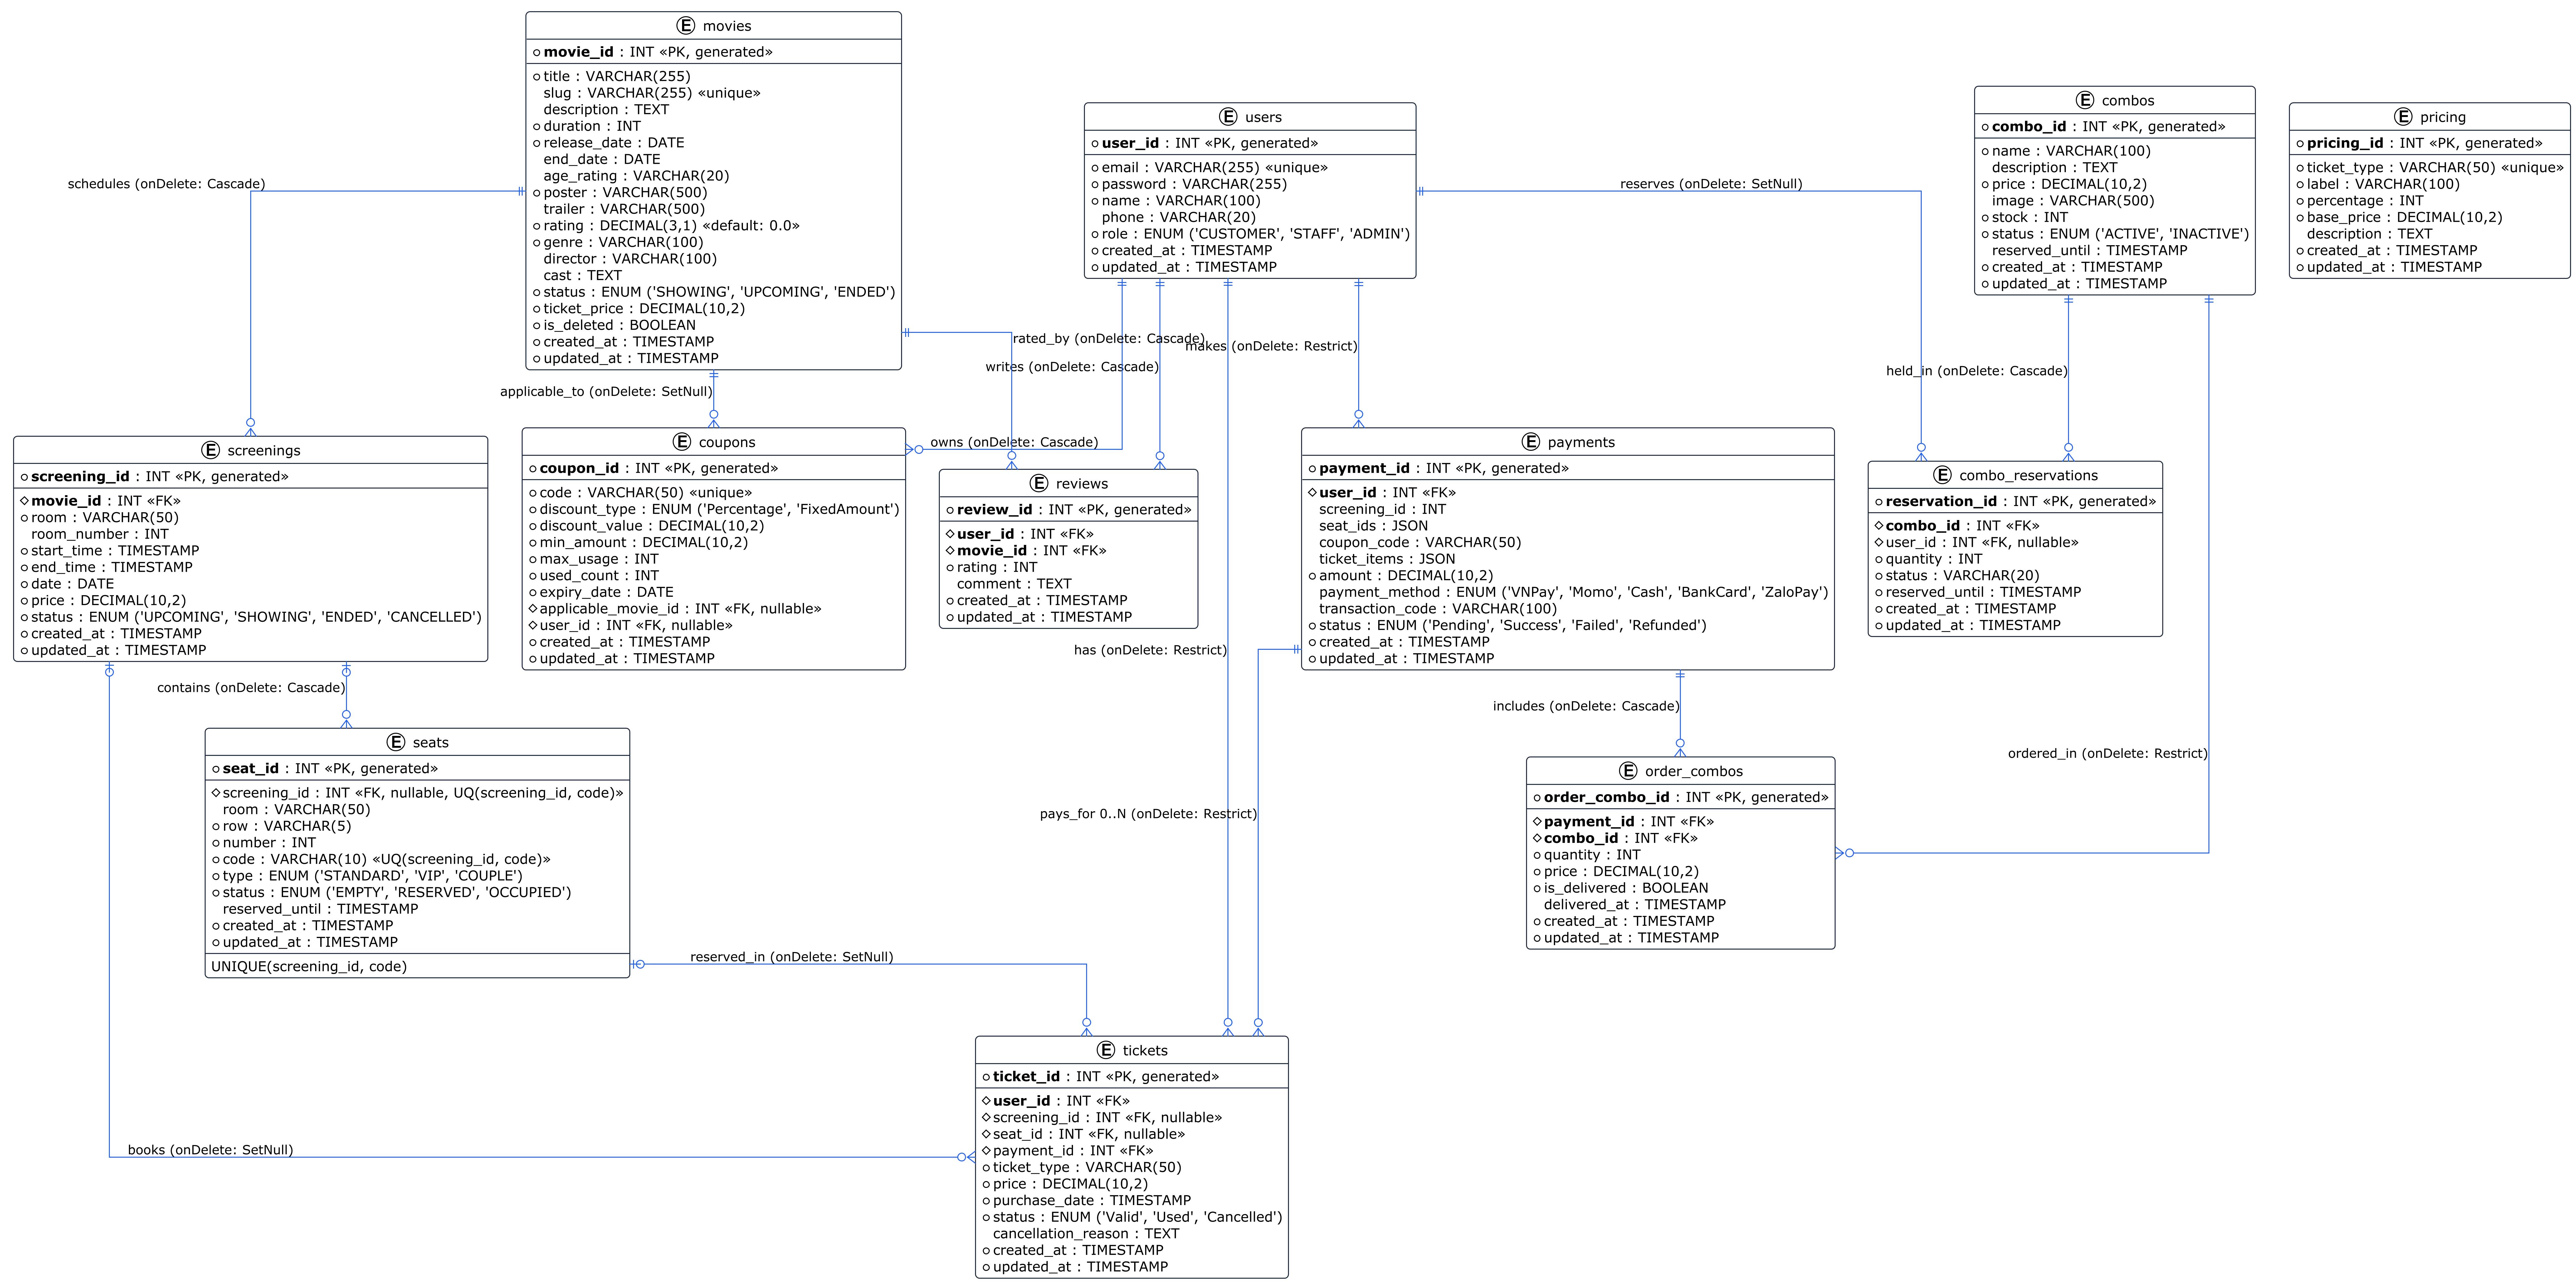
\includegraphics[width=\textwidth,height=0.80\textheight,keepaspectratio]{images/db/ERD_LumiCinema.png}
  \caption{Sơ đồ thực thể kết hợp (ERD) hệ thống LumiCinema}
  \label{fig:erd}
\end{figure}

\begin{figure}[H]
  \centering
  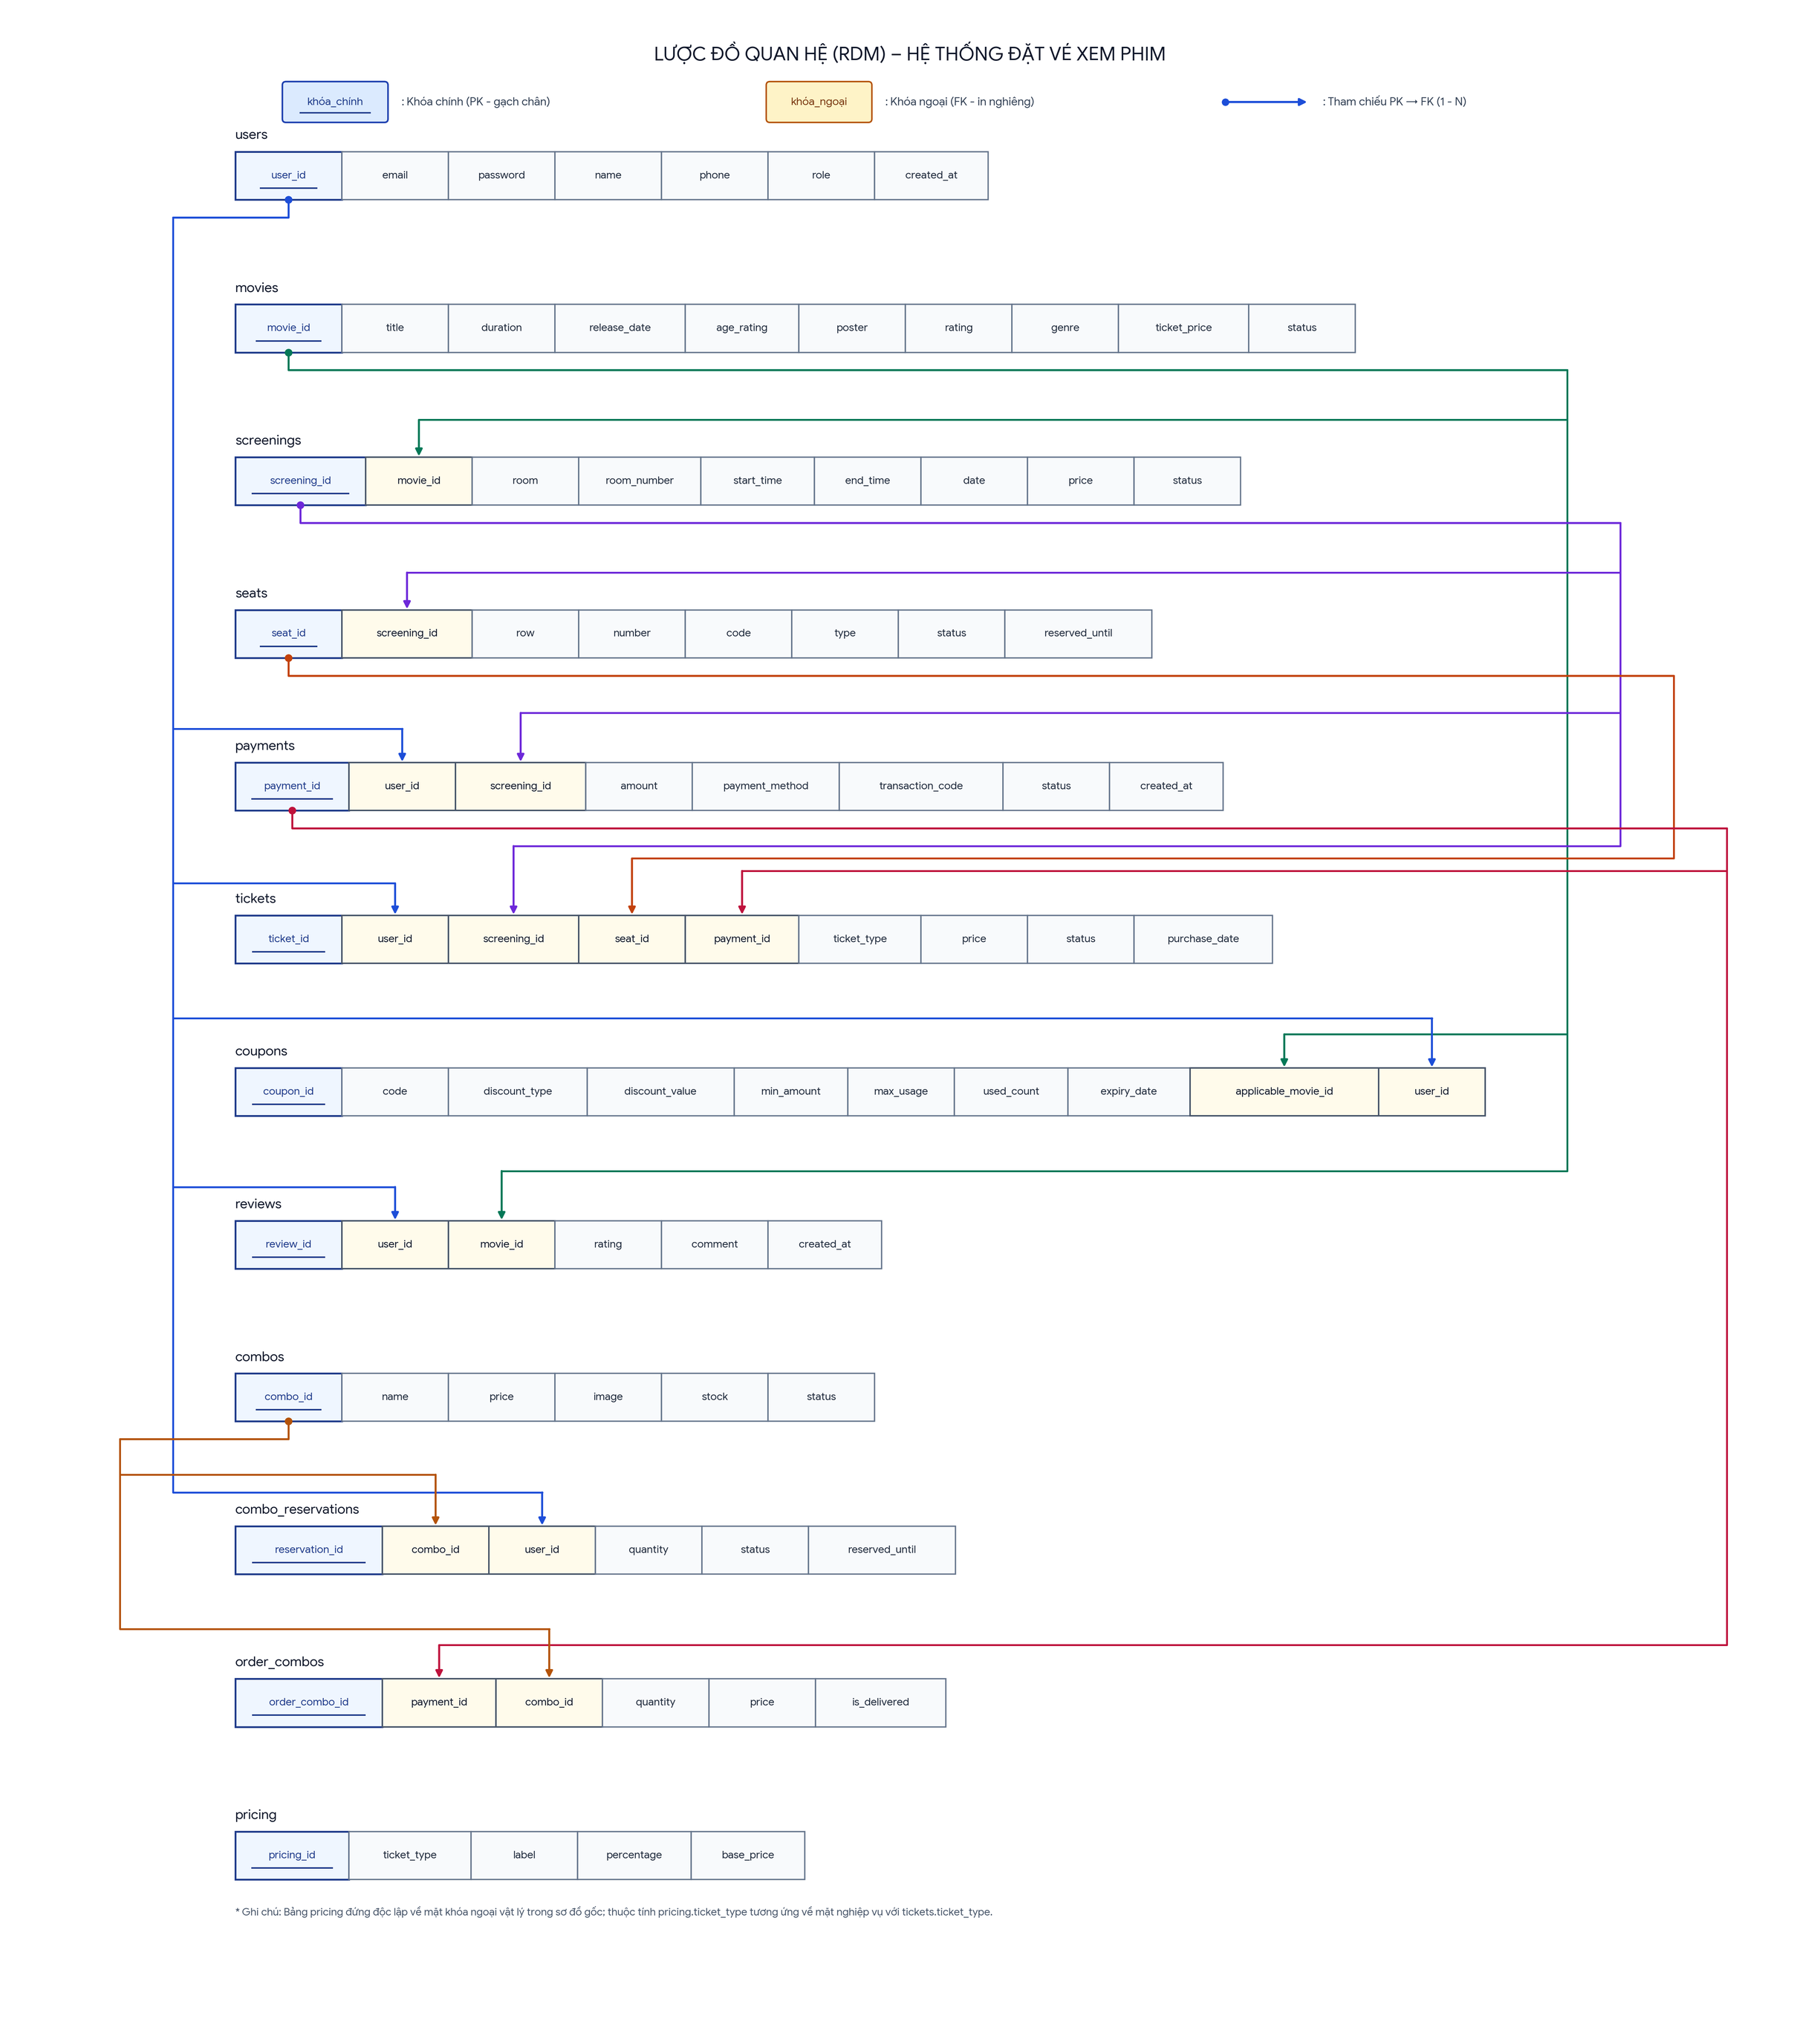
\includegraphics[width=\textwidth,height=0.80\textheight,keepaspectratio]{images/db/rdm_diagram.png}
  \caption{Mô hình dữ liệu quan hệ (RDM) hệ thống LumiCinema}
  \label{fig:rdm}
\end{figure}

\subsection{Danh sách các kiểu liệt kê (Enum)}
\begin{longtable}{|p{4.0cm}|p{11.5cm}|}
\hline
\rowcolor{headerblue} \textbf{Tên Enum} & \textbf{Các giá trị hợp lệ} \\ \hline
\endhead
\textbf{Role} & \texttt{CUSTOMER, STAFF, ADMIN} \\ \hline
\textbf{MovieStatus} & \texttt{SHOWING // Đang chiếu, UPCOMING // Sắp chiếu, ENDED // Ngừng chiếu} \\ \hline
\textbf{ScreeningStatus} & \texttt{UPCOMING, SHOWING, ENDED, CANCELLED} \\ \hline
\textbf{SeatType} & \texttt{STANDARD // Ghế thường, VIP // Ghế VIP, COUPLE // Ghế đôi (Sweetbox)} \\ \hline
\textbf{SeatStatus} & \texttt{EMPTY, RESERVED, OCCUPIED} \\ \hline
\textbf{DiscountType} & \texttt{Percentage // Giảm theo \%, FixedAmount // Giảm theo số tiền cố định} \\ \hline
\textbf{PaymentMethod} & \texttt{VNPay, Momo, Cash, BankCard, ZaloPay} \\ \hline
\textbf{PaymentStatus} & \texttt{Pending // Đang chờ thanh toán, Success // Thanh toán thành công, Failed // Thất bại, Refunded // Đã hoàn tiền} \\ \hline
\textbf{TicketStatus} & \texttt{Valid // Vé hợp lệ, Used // Đã check-in / đã sử dụng, Cancelled // Đã hủy / đã bồi hoàn} \\ \hline
\textbf{ComboStatus} & \texttt{ACTIVE, INACTIVE} \\ \hline
\end{longtable}

\subsection{Mô tả chi tiết 12 bảng dữ liệu}
\subsubsection{Bảng \texttt{User}}
\begin{longtable}{|p{3.6cm}|p{3.0cm}|p{8.9cm}|}
\hline
\rowcolor{headerblue} \textbf{Tên cột} & \textbf{Kiểu dữ liệu} & \textbf{Ràng buộc / Ghi chú} \\ \hline
\endhead
\texttt{id} & \texttt{Int} & \small @id @default(autoincrement()) @map("user\_id") \\ \hline
\texttt{email} & \texttt{String} & \small @unique @db.VarChar(255) \\ \hline
\texttt{password} & \texttt{String} & \small @db.VarChar(255) \\ \hline
\texttt{name} & \texttt{String} & \small @db.VarChar(100) \\ \hline
\texttt{role} & \texttt{Role} & \small @default(CUSTOMER) \\ \hline
\texttt{createdAt} & \texttt{DateTime} & \small @default(now()) @map("created\_at") \\ \hline
\texttt{updatedAt} & \texttt{DateTime} & \small @updatedAt @map("updated\_at") \\ \hline
\end{longtable}

\subsubsection{Bảng \texttt{Movie}}
\begin{longtable}{|p{3.6cm}|p{3.0cm}|p{8.9cm}|}
\hline
\rowcolor{headerblue} \textbf{Tên cột} & \textbf{Kiểu dữ liệu} & \textbf{Ràng buộc / Ghi chú} \\ \hline
\endhead
\texttt{id} & \texttt{Int} & \small @id @default(autoincrement()) @map("movie\_id") \\ \hline
\texttt{title} & \texttt{String} & \small @db.VarChar(255) \\ \hline
\texttt{duration} & \texttt{Int} & \small // Thời lượng (phút) \\ \hline
\texttt{releaseDate} & \texttt{DateTime} & \small @map("release\_date") @db.Date \\ \hline
\texttt{poster} & \texttt{String} & \small @db.VarChar(500) \\ \hline
\texttt{rating} & \texttt{Decimal} & \small @default(0.0) @db.Decimal(3, 1) \\ \hline
\texttt{genre} & \texttt{String} & \small @db.VarChar(100) \\ \hline
\texttt{status} & \texttt{MovieStatus} & \small @default(SHOWING) \\ \hline
\texttt{ticketPrice} & \texttt{Decimal} & \small @default(120000) @map("ticket\_price") @db.Decimal(10, 2) \\ \hline
\texttt{isDeleted} & \texttt{Boolean} & \small @default(false) @map("is\_deleted") \\ \hline
\texttt{createdAt} & \texttt{DateTime} & \small @default(now()) @map("created\_at") \\ \hline
\texttt{updatedAt} & \texttt{DateTime} & \small @updatedAt @map("updated\_at") \\ \hline
\end{longtable}

\subsubsection{Bảng \texttt{Screening}}
\begin{longtable}{|p{3.6cm}|p{3.0cm}|p{8.9cm}|}
\hline
\rowcolor{headerblue} \textbf{Tên cột} & \textbf{Kiểu dữ liệu} & \textbf{Ràng buộc / Ghi chú} \\ \hline
\endhead
\texttt{id} & \texttt{Int} & \small @id @default(autoincrement()) @map("screening\_id") \\ \hline
\texttt{movieId} & \texttt{Int} & \small @map("movie\_id") \\ \hline
\texttt{room} & \texttt{String} & \small @db.VarChar(50) // Vd: "Cinema 01", "Cinema 02" \\ \hline
\texttt{startTime} & \texttt{DateTime} & \small @map("start\_time") \\ \hline
\texttt{endTime} & \texttt{DateTime} & \small @map("end\_time") \\ \hline
\texttt{date} & \texttt{DateTime} & \small @db.Date \\ \hline
\texttt{price} & \texttt{Decimal} & \small @db.Decimal(10, 2) \\ \hline
\texttt{status} & \texttt{ScreeningStatus} & \small @default(UPCOMING) \\ \hline
\texttt{createdAt} & \texttt{DateTime} & \small @default(now()) @map("created\_at") \\ \hline
\texttt{updatedAt} & \texttt{DateTime} & \small @updatedAt @map("updated\_at") \\ \hline
\texttt{movie} & \texttt{Movie} & \small @relation(fields: [movieId], references: [id], onDelete: Cascade) \\ \hline
\end{longtable}

\subsubsection{Bảng \texttt{Seat}}
\begin{longtable}{|p{3.6cm}|p{3.0cm}|p{8.9cm}|}
\hline
\rowcolor{headerblue} \textbf{Tên cột} & \textbf{Kiểu dữ liệu} & \textbf{Ràng buộc / Ghi chú} \\ \hline
\endhead
\texttt{id} & \texttt{Int} & \small @id @default(autoincrement()) @map("seat\_id") \\ \hline
\texttt{row} & \texttt{String} & \small @db.VarChar(5) // Vd: "A", "B", "C" \\ \hline
\texttt{number} & \texttt{Int} & \small // Vd: 1, 2, 3 \\ \hline
\texttt{code} & \texttt{String} & \small @db.VarChar(10) // Vd: "A1", "A2", "C10" \\ \hline
\texttt{type} & \texttt{SeatType} & \small @default(STANDARD) \\ \hline
\texttt{status} & \texttt{SeatStatus} & \small @default(EMPTY) \\ \hline
\texttt{createdAt} & \texttt{DateTime} & \small @default(now()) @map("created\_at") \\ \hline
\texttt{updatedAt} & \texttt{DateTime} & \small @updatedAt @map("updated\_at") \\ \hline
\texttt{screening} & \texttt{Screening?} & \small @relation(fields: [screeningId], references: [id], onDelete: Cascade) \\ \hline
\end{longtable}

\subsubsection{Bảng \texttt{Pricing}}
\begin{longtable}{|p{3.6cm}|p{3.0cm}|p{8.9cm}|}
\hline
\rowcolor{headerblue} \textbf{Tên cột} & \textbf{Kiểu dữ liệu} & \textbf{Ràng buộc / Ghi chú} \\ \hline
\endhead
\texttt{id} & \texttt{Int} & \small @id @default(autoincrement()) @map("pricing\_id") \\ \hline
\texttt{ticketType} & \texttt{String} & \small @unique @map("ticket\_type") @db.VarChar(50) // Vd: "Normal", "Child", "VIP" \\ \hline
\texttt{label} & \texttt{String} & \small @db.VarChar(100) // Vd: "Vé Thường", "Vé Trẻ Em" \\ \hline
\texttt{percentage} & \texttt{Int} & \small @default(100) // \% giá vé: 100\%, 50\%, 180\% \\ \hline
\texttt{basePrice} & \texttt{Decimal} & \small @map("base\_price") @db.Decimal(10, 2) \\ \hline
\texttt{createdAt} & \texttt{DateTime} & \small @default(now()) @map("created\_at") \\ \hline
\texttt{updatedAt} & \texttt{DateTime} & \small @updatedAt @map("updated\_at") \\ \hline
\end{longtable}

\subsubsection{Bảng \texttt{Coupon}}
\begin{longtable}{|p{3.6cm}|p{3.0cm}|p{8.9cm}|}
\hline
\rowcolor{headerblue} \textbf{Tên cột} & \textbf{Kiểu dữ liệu} & \textbf{Ràng buộc / Ghi chú} \\ \hline
\endhead
\texttt{id} & \texttt{Int} & \small @id @default(autoincrement()) @map("coupon\_id") \\ \hline
\texttt{code} & \texttt{String} & \small @unique @db.VarChar(50) \\ \hline
\texttt{discountType} & \texttt{DiscountType} & \small @map("discount\_type") \\ \hline
\texttt{discountValue} & \texttt{Decimal} & \small @map("discount\_value") @db.Decimal(10, 2) \\ \hline
\texttt{minAmount} & \texttt{Decimal} & \small @default(0) @map("min\_amount") @db.Decimal(10, 2) \\ \hline
\texttt{maxUsage} & \texttt{Int} & \small @default(1) @map("max\_usage") \\ \hline
\texttt{usedCount} & \texttt{Int} & \small @default(0) @map("used\_count") \\ \hline
\texttt{expiryDate} & \texttt{DateTime} & \small @map("expiry\_date") @db.Date \\ \hline
\texttt{createdAt} & \texttt{DateTime} & \small @default(now()) @map("created\_at") \\ \hline
\texttt{updatedAt} & \texttt{DateTime} & \small @updatedAt @map("updated\_at") \\ \hline
\texttt{movie} & \texttt{Movie?} & \small @relation(fields: [applicableMovieId], references: [id], onDelete: SetNull) \\ \hline
\texttt{user} & \texttt{User?} & \small @relation(fields: [userId], references: [id], onDelete: Cascade) \\ \hline
\end{longtable}

\subsubsection{Bảng \texttt{Combo}}
\begin{longtable}{|p{3.6cm}|p{3.0cm}|p{8.9cm}|}
\hline
\rowcolor{headerblue} \textbf{Tên cột} & \textbf{Kiểu dữ liệu} & \textbf{Ràng buộc / Ghi chú} \\ \hline
\endhead
\texttt{id} & \texttt{Int} & \small @id @default(autoincrement()) @map("combo\_id") \\ \hline
\texttt{name} & \texttt{String} & \small @db.VarChar(100) \\ \hline
\texttt{price} & \texttt{Decimal} & \small @db.Decimal(10, 2) \\ \hline
\texttt{stock} & \texttt{Int} & \small @default(100) \\ \hline
\texttt{status} & \texttt{ComboStatus} & \small @default(ACTIVE) \\ \hline
\texttt{createdAt} & \texttt{DateTime} & \small @default(now()) @map("created\_at") \\ \hline
\texttt{updatedAt} & \texttt{DateTime} & \small @updatedAt @map("updated\_at") \\ \hline
\end{longtable}

\subsubsection{Bảng \texttt{ComboReservation}}
\begin{longtable}{|p{3.6cm}|p{3.0cm}|p{8.9cm}|}
\hline
\rowcolor{headerblue} \textbf{Tên cột} & \textbf{Kiểu dữ liệu} & \textbf{Ràng buộc / Ghi chú} \\ \hline
\endhead
\texttt{id} & \texttt{Int} & \small @id @default(autoincrement()) @map("reservation\_id") \\ \hline
\texttt{comboId} & \texttt{Int} & \small @map("combo\_id") \\ \hline
\texttt{quantity} & \texttt{Int} & \small @default(1) \\ \hline
\texttt{status} & \texttt{String} & \small @default("RESERVED") @db.VarChar(20) // 'RESERVED' | 'RELEASED' | 'COMPLETED' \\ \hline
\texttt{reservedUntil} & \texttt{DateTime} & \small @map("reserved\_until") \\ \hline
\texttt{createdAt} & \texttt{DateTime} & \small @default(now()) @map("created\_at") \\ \hline
\texttt{updatedAt} & \texttt{DateTime} & \small @updatedAt @map("updated\_at") \\ \hline
\texttt{combo} & \texttt{Combo} & \small @relation(fields: [comboId], references: [id], onDelete: Cascade) \\ \hline
\texttt{user} & \texttt{User?} & \small @relation(fields: [userId], references: [id], onDelete: SetNull) \\ \hline
\end{longtable}

\subsubsection{Bảng \texttt{Payment}}
\begin{longtable}{|p{3.6cm}|p{3.0cm}|p{8.9cm}|}
\hline
\rowcolor{headerblue} \textbf{Tên cột} & \textbf{Kiểu dữ liệu} & \textbf{Ràng buộc / Ghi chú} \\ \hline
\endhead
\texttt{id} & \texttt{Int} & \small @id @default(autoincrement()) @map("payment\_id") \\ \hline
\texttt{userId} & \texttt{Int} & \small @map("user\_id") \\ \hline
\texttt{amount} & \texttt{Decimal} & \small @db.Decimal(10, 2) \\ \hline
\texttt{status} & \texttt{PaymentStatus} & \small @default(Pending) \\ \hline
\texttt{createdAt} & \texttt{DateTime} & \small @default(now()) @map("created\_at") \\ \hline
\texttt{updatedAt} & \texttt{DateTime} & \small @updatedAt @map("updated\_at") \\ \hline
\texttt{user} & \texttt{User} & \small @relation(fields: [userId], references: [id], onDelete: Restrict) \\ \hline
\end{longtable}

\subsubsection{Bảng \texttt{Ticket}}
\begin{longtable}{|p{3.6cm}|p{3.0cm}|p{8.9cm}|}
\hline
\rowcolor{headerblue} \textbf{Tên cột} & \textbf{Kiểu dữ liệu} & \textbf{Ràng buộc / Ghi chú} \\ \hline
\endhead
\texttt{id} & \texttt{Int} & \small @id @default(autoincrement()) @map("ticket\_id") \\ \hline
\texttt{userId} & \texttt{Int} & \small @map("user\_id") \\ \hline
\texttt{paymentId} & \texttt{Int} & \small @map("payment\_id") \\ \hline
\texttt{ticketType} & \texttt{String} & \small @map("ticket\_type") @db.VarChar(50) \\ \hline
\texttt{price} & \texttt{Decimal} & \small @db.Decimal(10, 2) \\ \hline
\texttt{purchaseDate} & \texttt{DateTime} & \small @default(now()) @map("purchase\_date") \\ \hline
\texttt{status} & \texttt{TicketStatus} & \small @default(Valid) \\ \hline
\texttt{createdAt} & \texttt{DateTime} & \small @default(now()) @map("created\_at") \\ \hline
\texttt{updatedAt} & \texttt{DateTime} & \small @updatedAt @map("updated\_at") \\ \hline
\texttt{user} & \texttt{User} & \small @relation(fields: [userId], references: [id], onDelete: Restrict) \\ \hline
\texttt{screening} & \texttt{Screening?} & \small @relation(fields: [screeningId], references: [id], onDelete: SetNull) \\ \hline
\texttt{seat} & \texttt{Seat?} & \small @relation(fields: [seatId], references: [id], onDelete: SetNull) \\ \hline
\texttt{payment} & \texttt{Payment} & \small @relation(fields: [paymentId], references: [id], onDelete: Restrict) \\ \hline
\end{longtable}

\subsubsection{Bảng \texttt{OrderCombo}}
\begin{longtable}{|p{3.6cm}|p{3.0cm}|p{8.9cm}|}
\hline
\rowcolor{headerblue} \textbf{Tên cột} & \textbf{Kiểu dữ liệu} & \textbf{Ràng buộc / Ghi chú} \\ \hline
\endhead
\texttt{id} & \texttt{Int} & \small @id @default(autoincrement()) @map("order\_combo\_id") \\ \hline
\texttt{paymentId} & \texttt{Int} & \small @map("payment\_id") \\ \hline
\texttt{comboId} & \texttt{Int} & \small @map("combo\_id") \\ \hline
\texttt{quantity} & \texttt{Int} & \small Thuộc tính dữ liệu \\ \hline
\texttt{price} & \texttt{Decimal} & \small @db.Decimal(10, 2) // Giá combo tại thời điểm mua \\ \hline
\texttt{isDelivered} & \texttt{Boolean} & \small @default(false) @map("is\_delivered") \\ \hline
\texttt{createdAt} & \texttt{DateTime} & \small @default(now()) @map("created\_at") \\ \hline
\texttt{updatedAt} & \texttt{DateTime} & \small @updatedAt @map("updated\_at") \\ \hline
\texttt{payment} & \texttt{Payment} & \small @relation(fields: [paymentId], references: [id], onDelete: Cascade) \\ \hline
\texttt{combo} & \texttt{Combo} & \small @relation(fields: [comboId], references: [id], onDelete: Restrict) \\ \hline
\end{longtable}

\subsubsection{Bảng \texttt{Review}}
\begin{longtable}{|p{3.6cm}|p{3.0cm}|p{8.9cm}|}
\hline
\rowcolor{headerblue} \textbf{Tên cột} & \textbf{Kiểu dữ liệu} & \textbf{Ràng buộc / Ghi chú} \\ \hline
\endhead
\texttt{id} & \texttt{Int} & \small @id @default(autoincrement()) @map("review\_id") \\ \hline
\texttt{userId} & \texttt{Int} & \small @map("user\_id") \\ \hline
\texttt{movieId} & \texttt{Int} & \small @map("movie\_id") \\ \hline
\texttt{rating} & \texttt{Int} & \small // 1 đến 5 sao \\ \hline
\texttt{createdAt} & \texttt{DateTime} & \small @default(now()) @map("created\_at") \\ \hline
\texttt{updatedAt} & \texttt{DateTime} & \small @updatedAt @map("updated\_at") \\ \hline
\texttt{user} & \texttt{User} & \small @relation(fields: [userId], references: [id], onDelete: Cascade) \\ \hline
\texttt{movie} & \texttt{Movie} & \small @relation(fields: [movieId], references: [id], onDelete: Cascade) \\ \hline
\end{longtable}


\section{Thiết kế giao diện người dùng (UI)}
Phần này trình bày hình ảnh giao diện thực tế của hệ thống LumiCinema kèm theo \textbf{Danh sách thành phần} và \textbf{Danh sách biến cố} tương ứng cho từng màn hình chính.

% --- 1. Trang chủ ---
\subsection{Màn hình Trang chủ}
\begin{figure}[H]
  \centering
  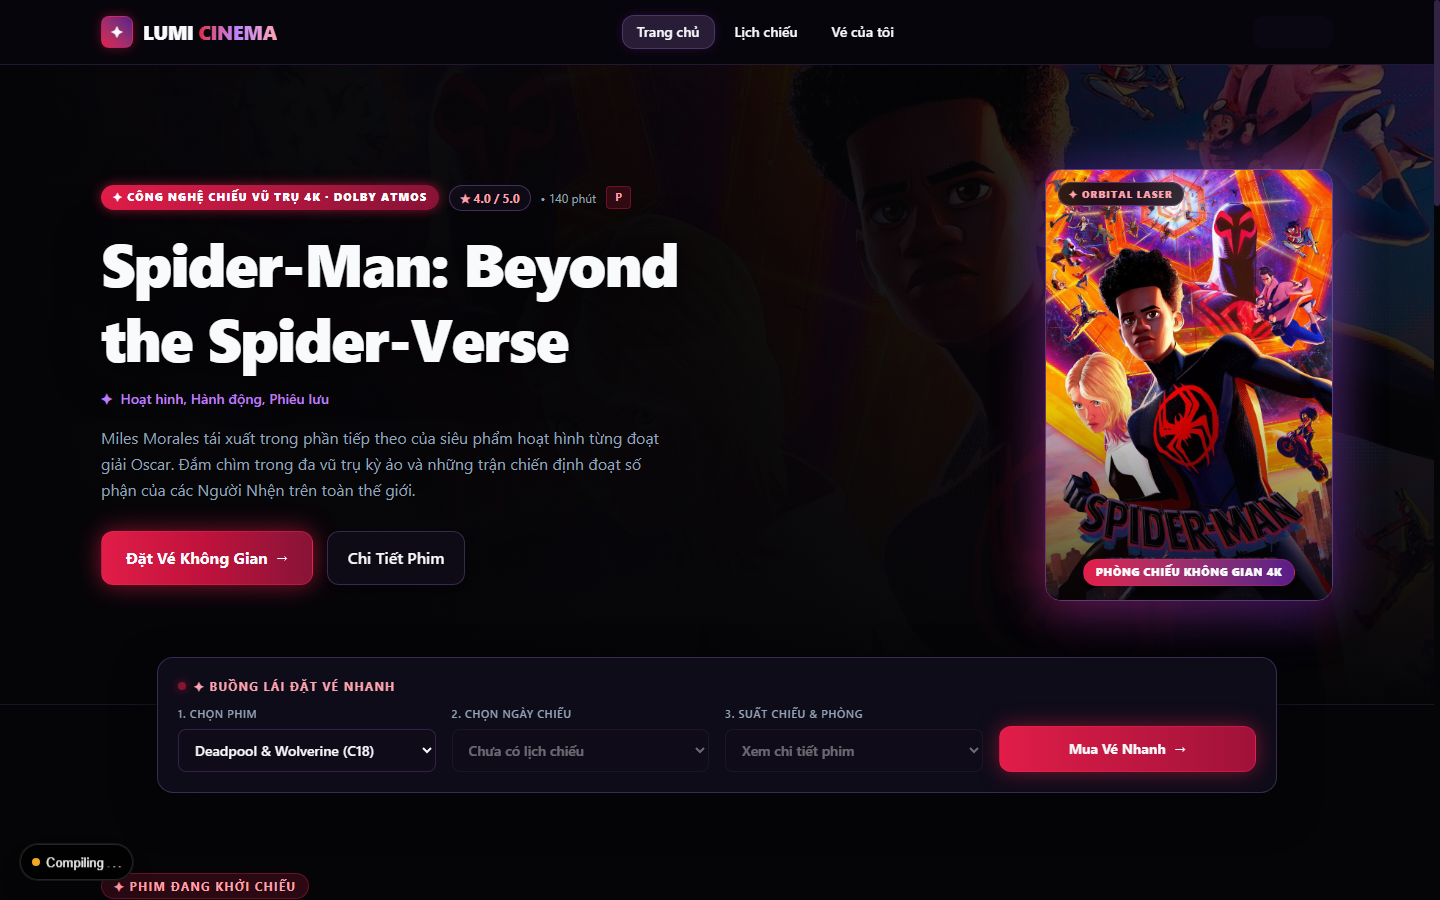
\includegraphics[width=\textwidth,height=0.55\textheight,keepaspectratio]{images/ui/ui_01_trang_chu.png}
  \caption{Giao diện Trang chủ LumiCinema}
  \label{fig:ui_01}
\end{figure}
\begin{itemize}[leftmargin=1.2cm]
  \item \textbf{Danh sách thành phần:} Thanh điều hướng (Logo, Phim, Vé của tôi, Đăng nhập/Đăng ký), Banner phim nổi bật, Thanh tìm kiếm \& lọc thể loại/trạng thái phim, Lưới thẻ phim (Poster, tên phim, thời lượng, đánh giá sao, nút Đặt vé).
  \item \textbf{Danh sách biến cố:} Nhấn chọn phim $\rightarrow$ chuyển trang Chi tiết phim; Nhập từ khóa/chọn bộ lọc $\rightarrow$ lọc danh sách phim theo thời gian thực; Nhấn Đăng nhập/Đăng ký $\rightarrow$ mở trang xác thực.
\end{itemize}

% --- 2. Đăng nhập ---
\subsection{Màn hình Đăng nhập}
\begin{figure}[H]
  \centering
  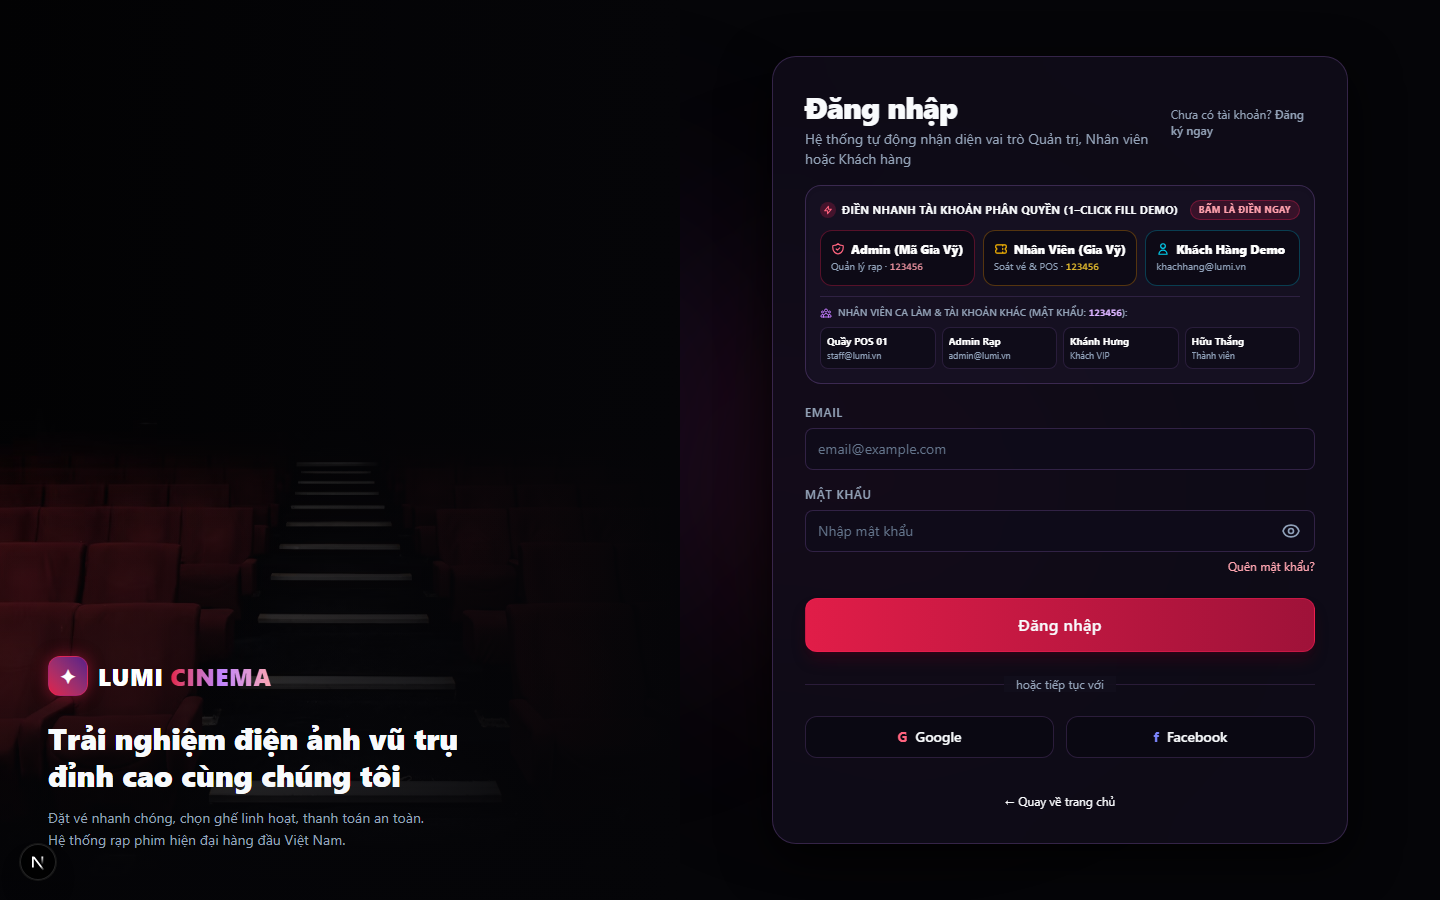
\includegraphics[width=\textwidth,height=0.55\textheight,keepaspectratio]{images/ui/ui_02_dang_nhap.png}
  \caption{Giao diện Đăng nhập}
  \label{fig:ui_02}
\end{figure}
\begin{itemize}[leftmargin=1.2cm]
  \item \textbf{Danh sách thành phần:} Ô nhập Email, Ô nhập Mật khẩu, Nút Đăng nhập, Liên kết chuyển sang trang Đăng ký, Vùng hiển thị thông báo lỗi.
  \item \textbf{Danh sách biến cố:} Nhấn ``Đăng nhập'' $\rightarrow$ gọi \texttt{POST /api/auth/login}, xác thực mật khẩu, lưu phiên làm việc (JWT Cookie) và điều hướng theo vai trò (Khách hàng / Nhân viên / Admin).
\end{itemize}

% --- 3. Đăng ký ---
\subsection{Màn hình Đăng ký tài khoản}
\begin{figure}[H]
  \centering
  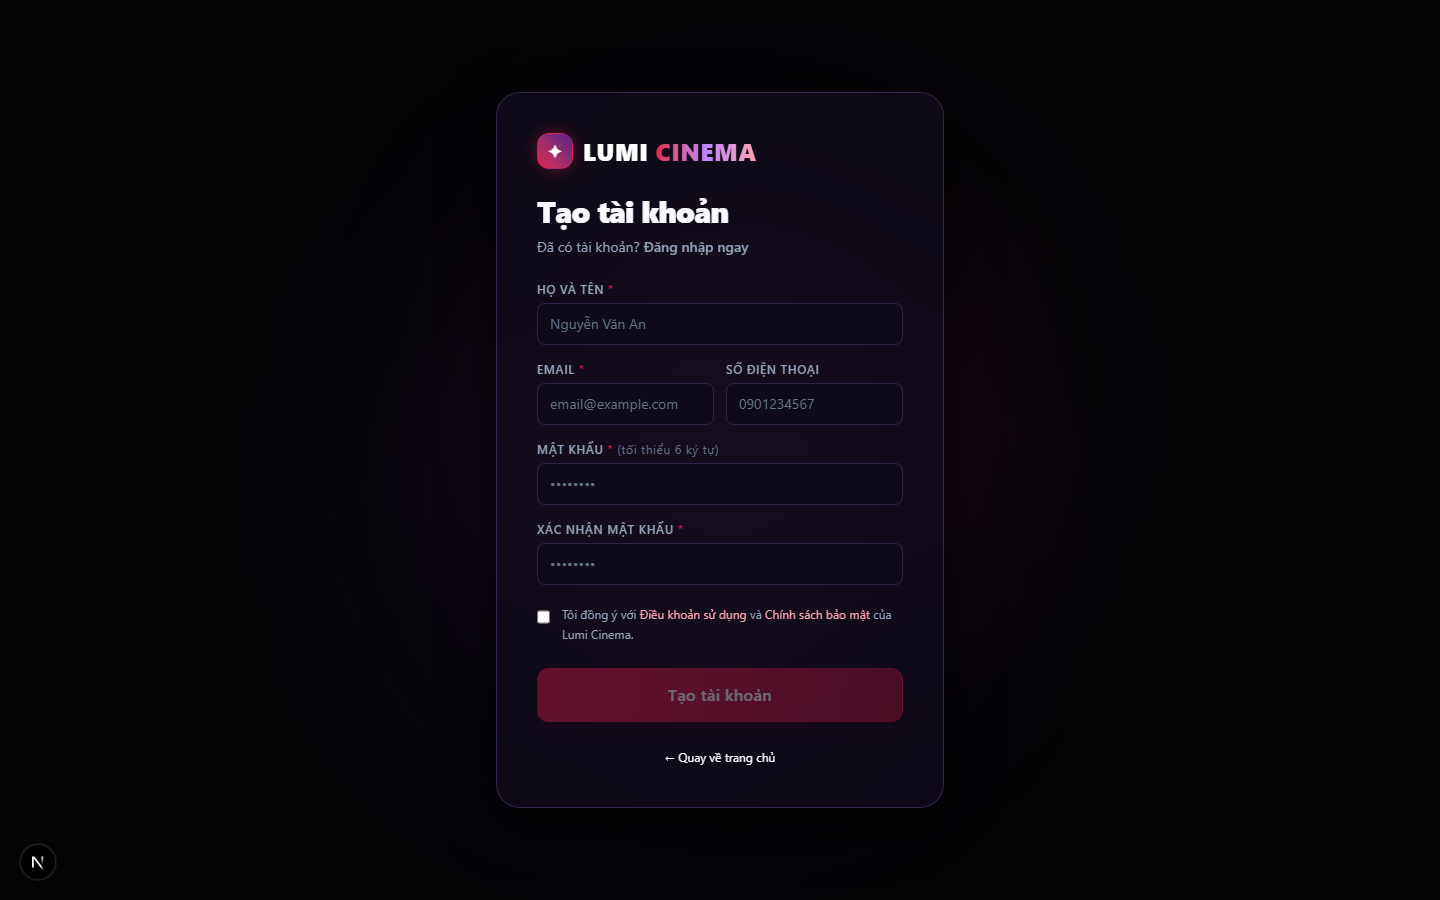
\includegraphics[width=\textwidth,height=0.55\textheight,keepaspectratio]{images/ui/ui_03_dang_ky.png}
  \caption{Giao diện Đăng ký tài khoản}
  \label{fig:ui_03}
\end{figure}
\begin{itemize}[leftmargin=1.2cm]
  \item \textbf{Danh sách thành phần:} Ô nhập Họ tên, Email, Số điện thoại, Mật khẩu, Xác nhận mật khẩu, Nút Đăng ký.
  \item \textbf{Danh sách biến cố:} Nhấn ``Đăng ký'' $\rightarrow$ kiểm tra hợp lệ dữ liệu, gọi \texttt{POST /api/auth/register}, mã hóa mật khẩu bằng bcrypt và tạo tài khoản khách hàng mới.
\end{itemize}

% --- 4. Chi tiết phim ---
\subsection{Màn hình Chi tiết phim và Chọn suất chiếu}
\begin{figure}[H]
  \centering
  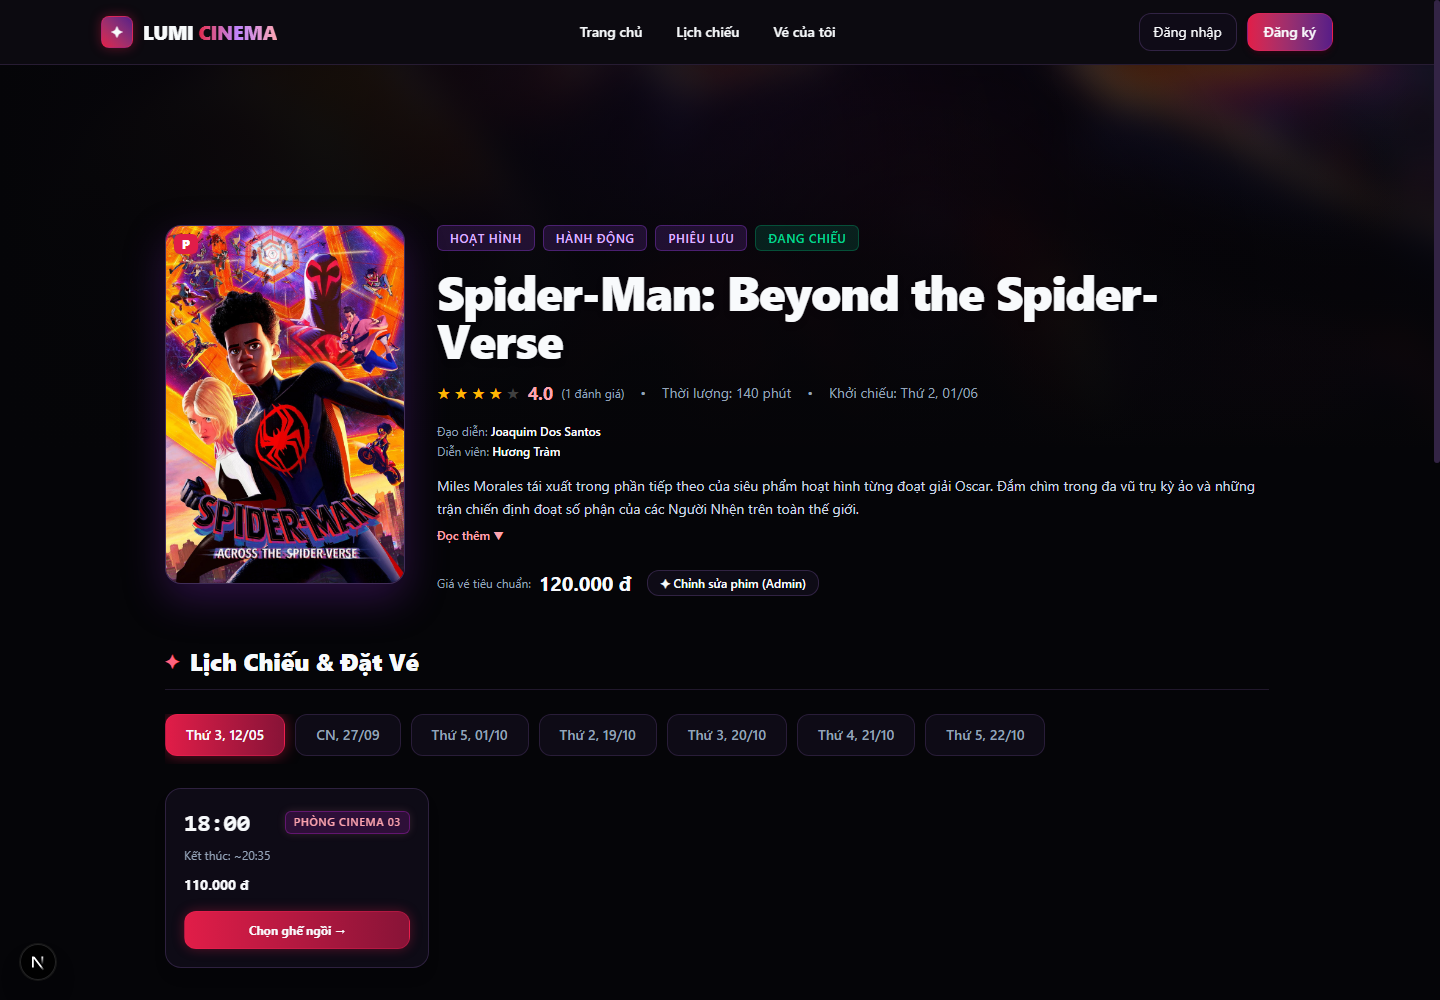
\includegraphics[width=\textwidth,height=0.55\textheight,keepaspectratio]{images/ui/ui_04_chi_tiet_phim.png}
  \caption{Giao diện Chi tiết phim và Suất chiếu}
  \label{fig:ui_04}
\end{figure}
\begin{itemize}[leftmargin=1.2cm]
  \item \textbf{Danh sách thành phần:} Poster, Thông tin phim (thể loại, thời lượng, mô tả, điểm đánh giá trung bình), Bộ chọn ngày chiếu, Danh sách nút khung giờ suất chiếu, Khu vực đánh giá phim (1--5 sao và bình luận).
  \item \textbf{Danh sách biến cố:} Chọn ngày chiếu $\rightarrow$ cập nhật danh sách suất chiếu; Nhấn khung giờ $\rightarrow$ chuyển sang màn hình Chọn ghế; Gửi đánh giá $\rightarrow$ gọi \texttt{POST /api/reviews}.
\end{itemize}

% --- 5. Chọn ghế ---
\subsection{Màn hình Chọn ghế (Sơ đồ 50 ghế A1--E10)}
\begin{figure}[H]
  \centering
  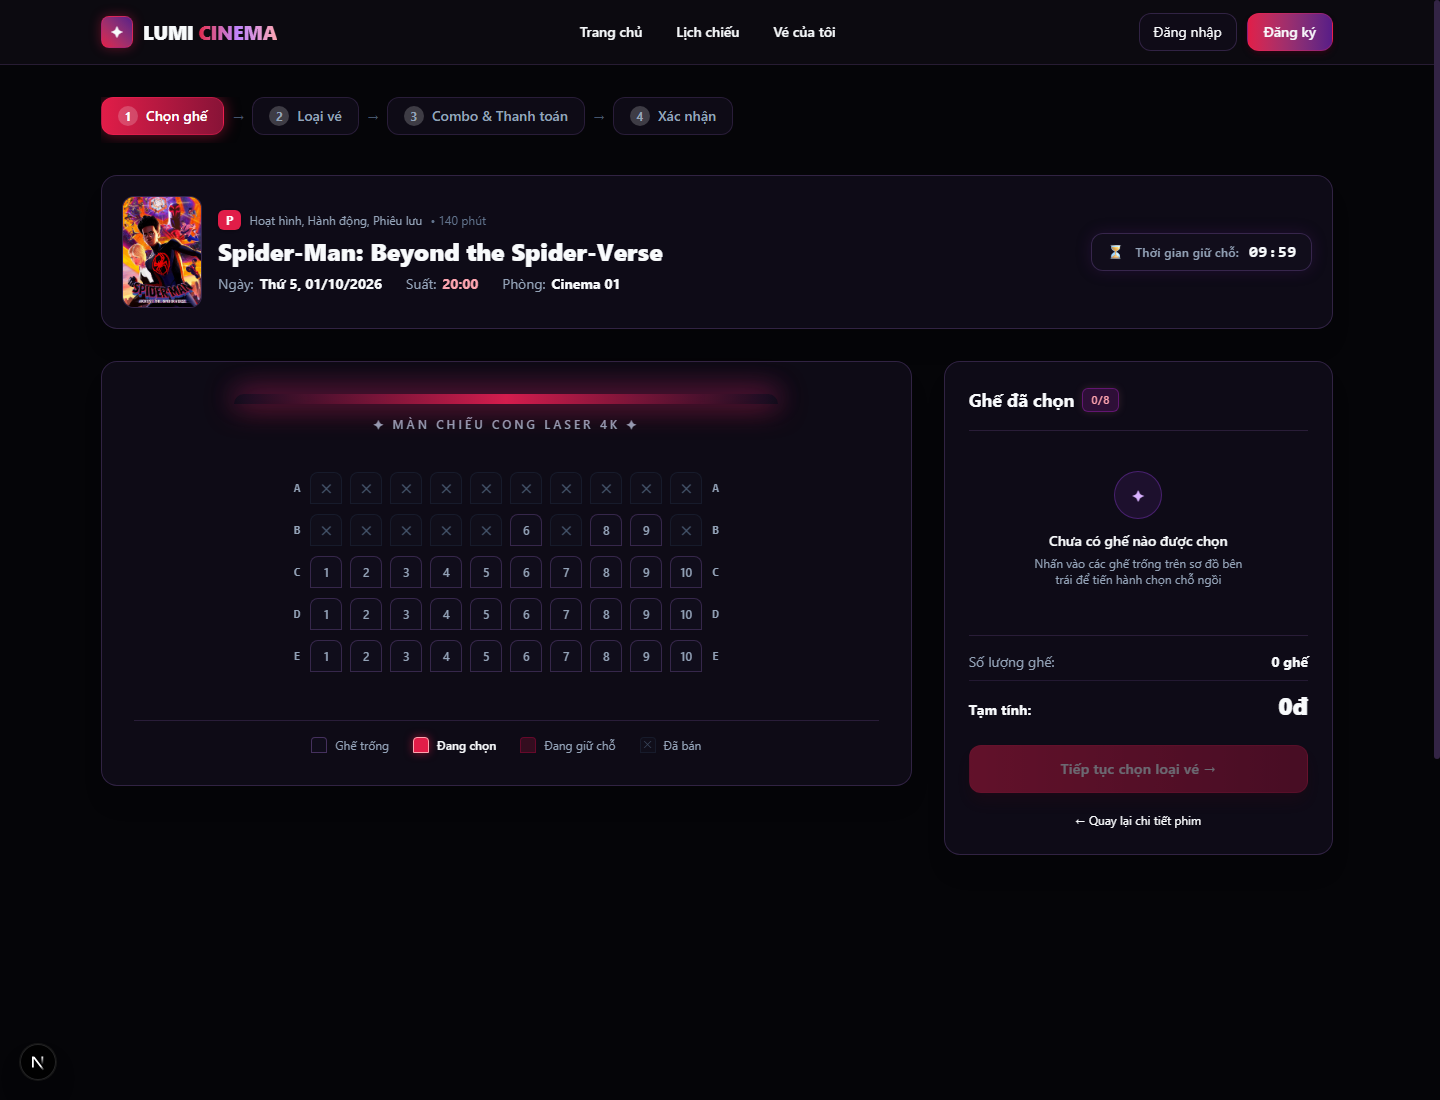
\includegraphics[width=\textwidth,height=0.55\textheight,keepaspectratio]{images/ui/ui_05_chon_ghe.png}
  \caption{Giao diện Chọn ghế phòng chiếu (5 hàng A--E, 10 cột 1--10)}
  \label{fig:ui_05}
\end{figure}
\begin{itemize}[leftmargin=1.2cm]
  \item \textbf{Danh sách thành phần:} Thanh màn hình chiếu, Lưới 50 nút ghế (phân màu Trống / Đang chọn / Đang giữ / Đã đặt), Bộ chọn loại vé (Người lớn / Sinh viên / Trẻ em), Bảng tóm tắt ghế đã chọn \& tạm tính, Nút Tiếp tục.
  \item \textbf{Danh sách biến cố:} Nhấn chọn/bỏ chọn ghế $\rightarrow$ cập nhật danh sách ghế và tổng tiền; Nhấn ``Tiếp tục'' $\rightarrow$ giữ ghế tạm thời (TTL) và chuyển sang bước Chọn Combo.
\end{itemize}

% --- 6. Chọn Combo & Thanh toán ---
\subsection{Màn hình Chọn Combo, Áp dụng Voucher và Thanh toán}
\begin{figure}[H]
  \centering
  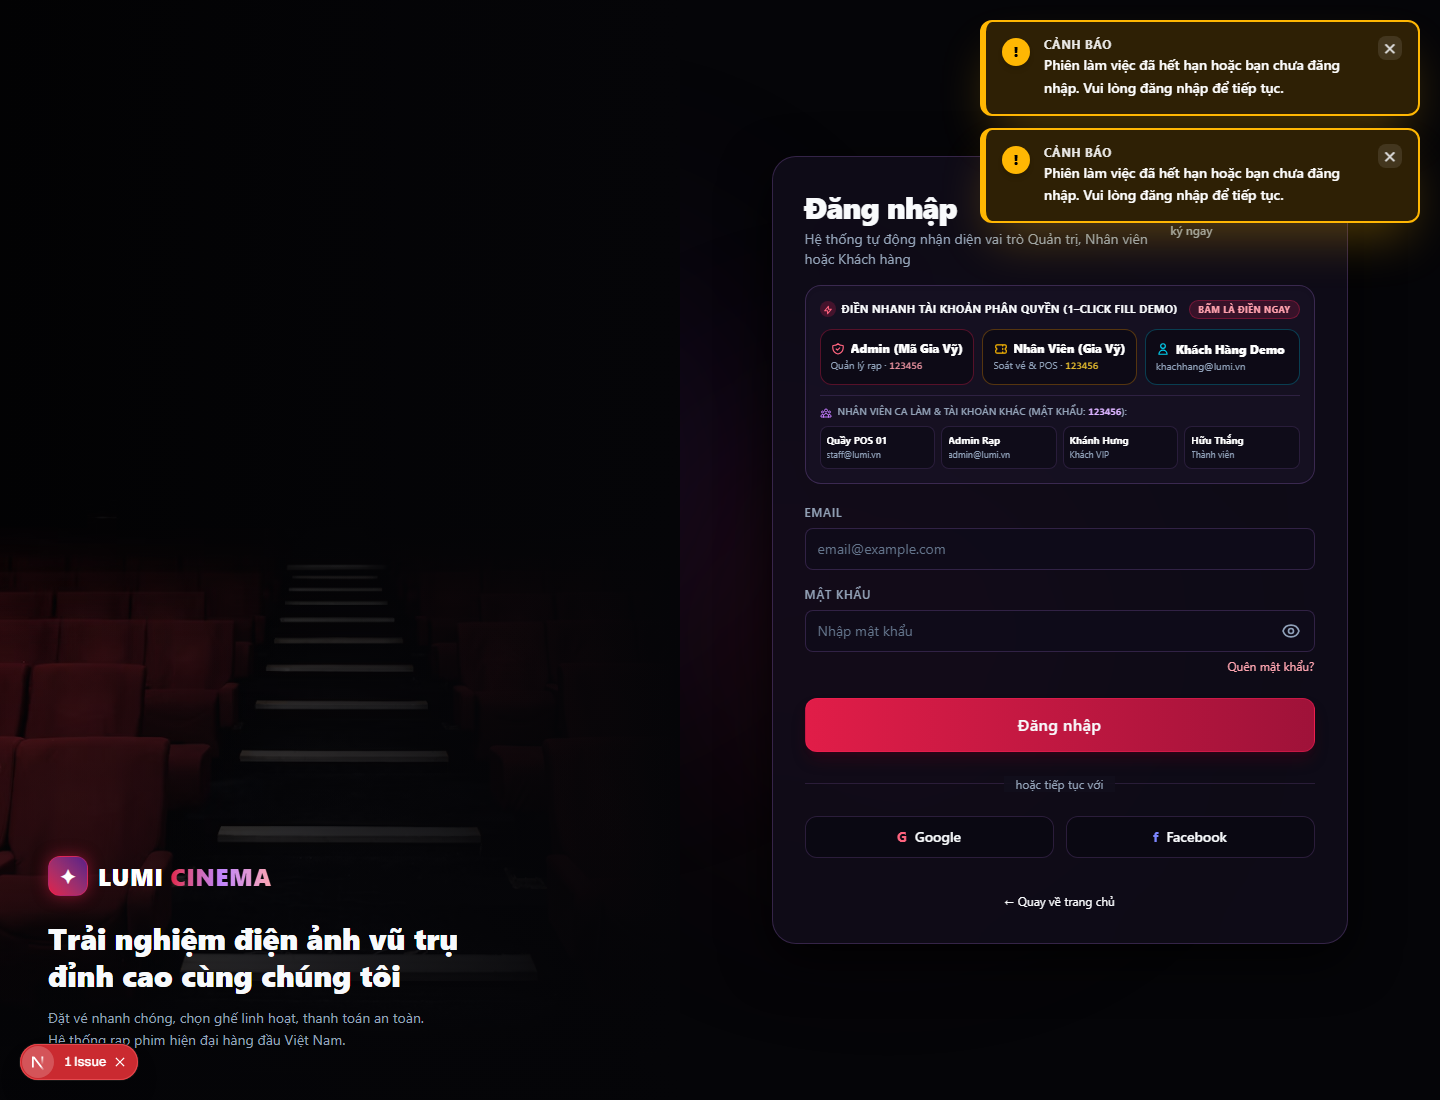
\includegraphics[width=\textwidth,height=0.55\textheight,keepaspectratio]{images/ui/ui_06_chon_combo.png}
  \caption{Giao diện Chọn Combo bắp nước và Thanh toán}
  \label{fig:ui_06}
\end{figure}
\begin{itemize}[leftmargin=1.2cm]
  \item \textbf{Danh sách thành phần:} Danh sách thẻ Combo (hình ảnh, giá, tồn kho, nút tăng/giảm số lượng), Ô nhập mã Voucher \& nút Áp dụng, Bộ chọn cổng thanh toán (ZaloPay / VNPay Gateway), Bảng tổng kết thanh toán, Nút Thanh toán.
  \item \textbf{Danh sách biến cố:} Tăng/giảm combo $\rightarrow$ cập nhật tổng tiền theo tồn kho; Áp dụng voucher $\rightarrow$ kiểm tra hợp lệ \& trừ giảm giá; Nhấn Thanh toán $\rightarrow$ tạo đơn và chuyển hướng sang cổng ZaloPay/VNPay (\texttt{/payments/zalopay-mock} hoặc \texttt{/payments/vnpay-mock}) để xác nhận trừ số dư.
\end{itemize}

% --- 7. Nhân viên POS ---
\subsection{Màn hình Nhân viên quầy (Bán vé, Soát vé \& Hủy vé sự cố)}
\begin{figure}[H]
  \centering
  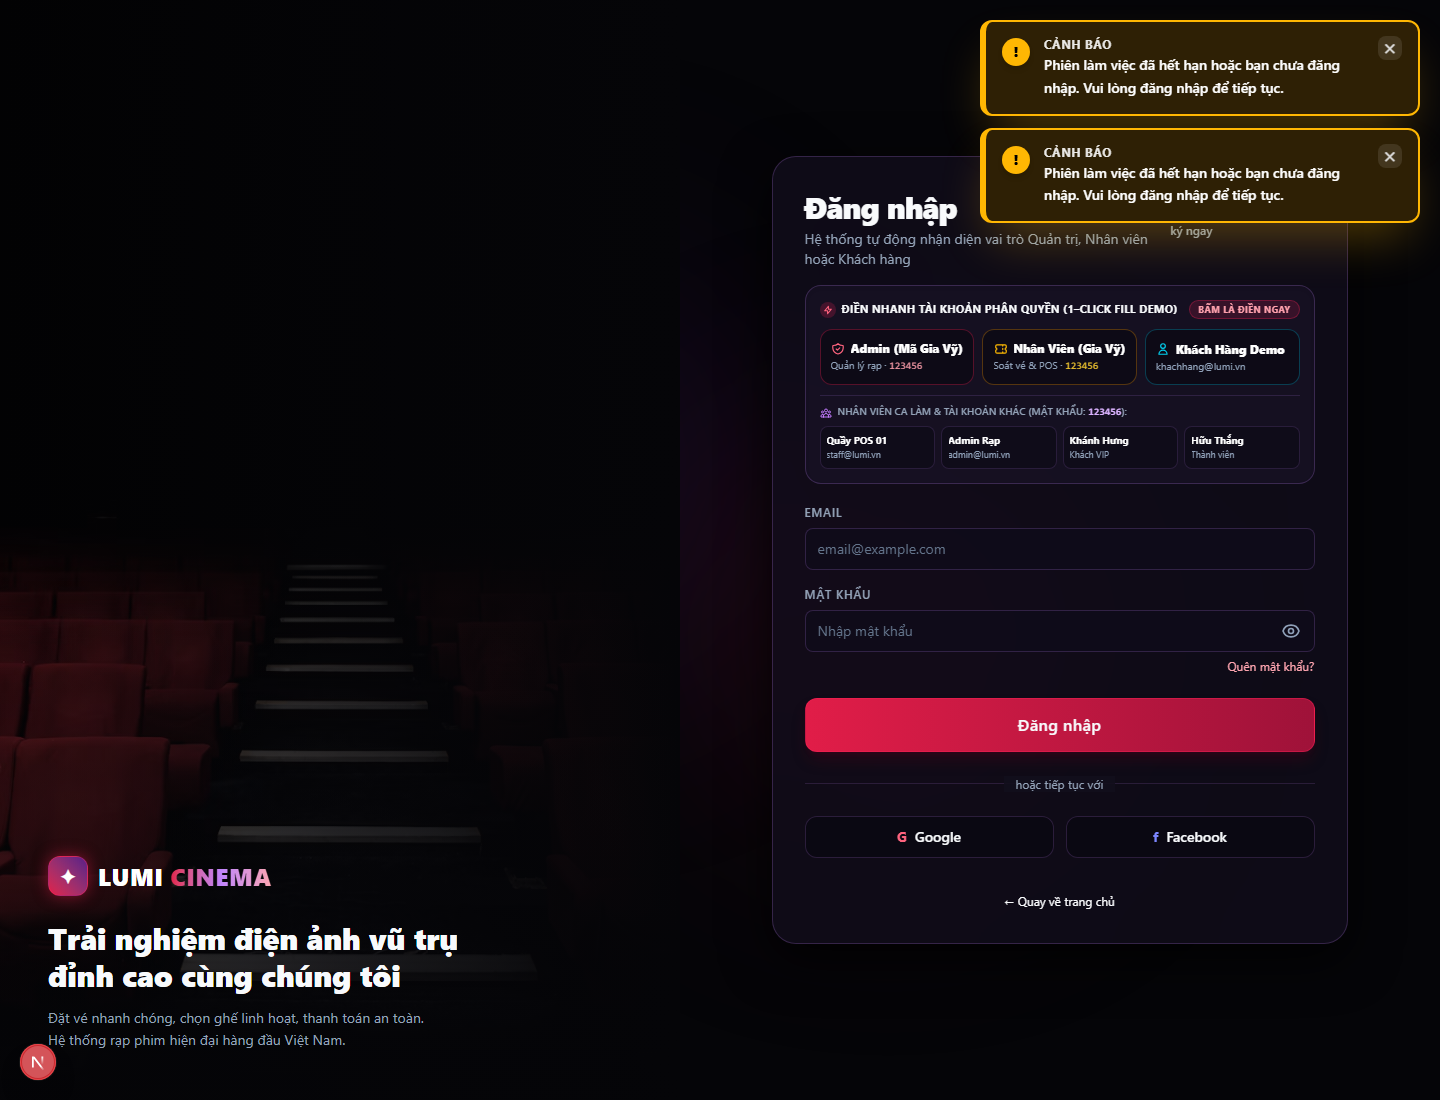
\includegraphics[width=\textwidth,height=0.55\textheight,keepaspectratio]{images/ui/ui_08_nhan_vien_staff.png}
  \caption{Giao diện làm việc của Nhân viên quầy (POS)}
  \label{fig:ui_08}
\end{figure}
\begin{itemize}[leftmargin=1.2cm]
  \item \textbf{Danh sách thành phần:} Các tab nghiệp vụ (Bán vé tại quầy, Soát vé \& Giao combo, Tra cứu \& Hủy vé), Ô tìm kiếm mã vé/SĐT, Sơ đồ ghế POS, Modal xử lý hủy vé sự cố 1 bước (chọn Hoàn 100\% tiền mặt hoặc Cấp voucher 100\%).
  \item \textbf{Danh sách biến cố:} Xác nhận bán vé $\rightarrow$ thu tiền, xuất vé; Quét/nhập mã vé $\rightarrow$ xác nhận vào rạp hoặc giao combo; Xác nhận ép hủy sự cố $\rightarrow$ giải phóng ghế, lưu log, lập chứng từ hoàn tiền/voucher và gửi email tự động.
\end{itemize}

% --- 8. Admin Dashboard ---
\subsection{Màn hình Quản trị và Báo cáo doanh thu (Admin Dashboard)}
\begin{figure}[H]
  \centering
  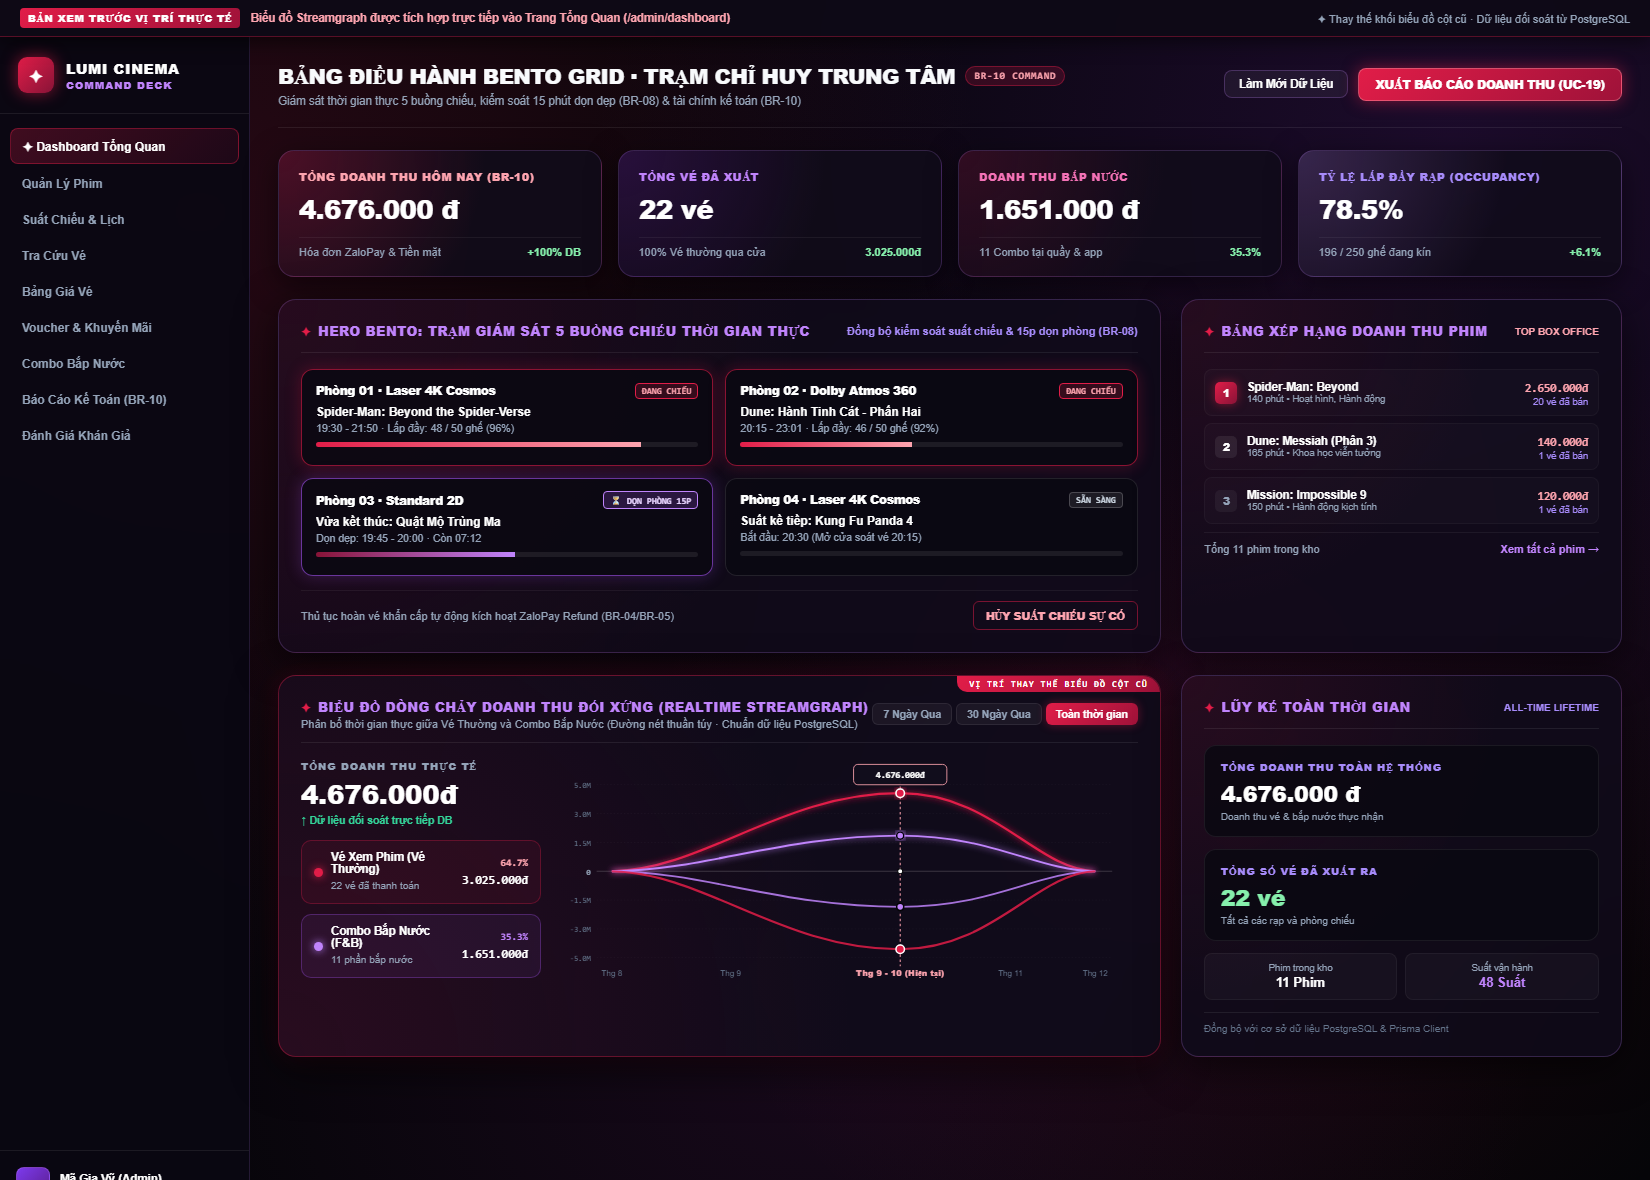
\includegraphics[width=\textwidth,height=0.55\textheight,keepaspectratio]{images/ui/ui_09_admin_dashboard_streamgraph.png}
  \caption{Giao diện Admin Dashboard với biểu đồ Streamgraph doanh thu}
  \label{fig:ui_09}
\end{figure}
\begin{itemize}[leftmargin=1.2cm]
  \item \textbf{Danh sách thành phần:} Thanh điều hướng quản trị (Dashboard, Phim, Suất chiếu, Combo, Voucher), Thẻ KPI tổng quan (Tổng doanh thu, Vé đã bán, Tỷ lệ lấp đầy), Biểu đồ Streamgraph doanh thu theo thời gian, Bộ lọc thời gian/phim/suất chiếu, Nút Xuất báo cáo CSV.
  \item \textbf{Danh sách biến cố:} Thay đổi bộ lọc $\rightarrow$ truy vấn lại số liệu tổng hợp vé \& combo; Nhấn ``Xuất CSV'' $\rightarrow$ tải về tệp báo cáo doanh thu định dạng CSV.
\end{itemize}


\chapter{CÀI ĐẶT VÀ THỬ NGHIỆM}
\section{Môi trường và Công nghệ cài đặt}
Hệ thống LumiCinema được xây dựng theo kiến trúc Full-stack hiện đại, đóng gói hoàn chỉnh bằng Docker để dễ dàng triển khai và chạy thử nghiệm đồng nhất trên mọi môi trường.

\begin{table}[H]
\centering
\caption{Ngăn xếp công nghệ sử dụng trong hệ thống LumiCinema}
\label{tab:tech_stack}
\renewcommand{\arraystretch}{1.25}
\begin{tabular}{|p{3.8cm}|p{11.4cm}|}
\hline
\rowcolor{headerblue} \textbf{Thành phần} & \textbf{Công nghệ / Phiên bản} \\ \hline
Framework \& Ngôn ngữ & Next.js 16 (App Router), React 19, TypeScript 5 \\ \hline
Giao diện (UI/UX) & Tailwind CSS, biểu đồ doanh thu trực quan Streamgraph \\ \hline
Cơ sở dữ liệu \& ORM & PostgreSQL 16, Prisma ORM (12 bảng, 10 enum, 15 khóa ngoại) \\ \hline
Xác thực \& Bảo mật & JWT (HTTP-only Cookie), mã hóa mật khẩu bcrypt, kiểm soát phân quyền theo vai trò (RBAC) \\ \hline
Cổng thanh toán & Cổng ZaloPay \& VNPay nội bộ (\texttt{/payments/zalopay-mock}, \texttt{/payments/vnpay-mock}) kèm API ví điện tử (\texttt{/api/payments/gateway-wallet}) hỗ trợ kiểm tra số dư (\texttt{INSUFFICIENT\_BALANCE}), nạp tiền (\texttt{topup}) và hoàn tiền tự động \\ \hline
Thông báo Email & Nodemailer (SMTP) gửi email xác nhận đặt vé, email cấp voucher bồi hoàn và email xác nhận hoàn 100\% tiền mặt \\ \hline
Triển khai (Deployment) & Docker \& Docker Compose (\texttt{lumicinema\_web}, \texttt{lumicinema\_db}) \\ \hline
\end{tabular}
\end{table}

\section{Kết quả thử nghiệm các chức năng chính}
Hệ thống đã được kiểm thử trên môi trường Docker thực tế (\texttt{http://localhost:3000}) với các kịch bản trọng yếu như Bảng~\ref{tab:test_results}.

\begin{longtable}{|p{1.2cm}|p{4.3cm}|p{6.8cm}|p{2.6cm}|}
\caption{Tổng hợp kết quả thử nghiệm các kịch bản nghiệp vụ chính} \label{tab:test_results} \\
\hline
\rowcolor{headerblue} \textbf{Mã TC} & \textbf{Kịch bản kiểm thử} & \textbf{Kết quả thực tế ghi nhận} & \textbf{Đánh giá} \\ \hline
\endhead
TC-01 & Đặt vé online + Combo + Voucher + ZaloPay/VNPay & Giữ ghế đúng TTL, trừ tồn kho combo, kiểm tra số dư ví Gateway (báo \texttt{INSUFFICIENT\_BALANCE} nếu thiếu, cho nạp thêm), thanh toán thành công và gửi email xác nhận vé. & \textbf{Đạt} \\ \hline
TC-02 & Chống đặt trùng ghế (Concurrency) & Khi hai phiên cùng chọn 1 ghế, chỉ phiên đầu giữ ghế thành công; phiên thứ hai nhận thông báo ghế đã được giữ/đặt. & \textbf{Đạt} \\ \hline
TC-03 & Khách hàng tự hủy vé ($\ge$ 2 giờ trước chiếu) & Kiểm tra điều kiện thời gian hợp lệ, chuyển trạng thái vé sang đã hủy, giải phóng ghế về trống, cấp mã voucher 50\% (hạn 30 ngày) và gửi email. & \textbf{Đạt} \\ \hline
TC-04 & Nhân viên ép hủy vé sự cố rạp (1 bước) & Hỗ trợ chọn Hoàn 100\% tiền mặt tại quầy hoặc Cấp voucher 100\%; tự động nhả ghế, ghi log nhân viên/lý do và gửi email thông báo tương ứng. & \textbf{Đạt} \\ \hline
TC-05 & Bán vé \& Soát vé tại quầy (POS) & Bán vé kèm combo, gắn khách hàng qua SĐT/Email, soát vé chuyển trạng thái đã vào rạp và cập nhật trạng thái đã giao combo. & \textbf{Đạt} \\ \hline
TC-06 & Quản trị danh mục \& Báo cáo doanh thu & Thêm suất chiếu tự động khởi tạo đúng 50 ghế (A1--E10); Dashboard hiển thị biểu đồ Streamgraph chính xác và xuất file CSV đầy đủ. & \textbf{Đạt} \\ \hline
\end{longtable}

\section{Đánh giá kết quả}
Toàn bộ các yêu cầu chức năng và phi chức năng trong tài liệu đặc tả SRS đều đã được hiện thực đầy đủ, hoạt động ổn định trên môi trường Docker. Đặc biệt, toàn bộ hệ thống tài liệu (SRS, Use Case, Sequence, Activity, State, Class, ERD, RDM) đã được rà soát và đồng bộ 100\% với mã nguồn thực tế.


\chapter{KẾT LUẬN VÀ HƯỚNG MỞ RỘNG}
\section{Kết luận}
Qua quá trình phân tích, thiết kế và cài đặt đồ án \textbf{Hệ thống quản lý bán vé xem phim LumiCinema}, Nhóm 10 đã hoàn thành các mục tiêu đề ra:
\begin{itemize}[leftmargin=1.2cm]
  \item Xây dựng hoàn chỉnh bộ hồ sơ phân tích thiết kế hướng đối tượng gồm BFD, 10 sơ đồ Use Case kèm đặc tả chi tiết, 38 sơ đồ Sequence, 17 lược đồ Activity, 6 sơ đồ State, sơ đồ Class (22 lớp), sơ đồ ERD và RDM (12 bảng, 10 enum, 15 khóa ngoại).
  \item Hiện thực thành công ứng dụng web LumiCinema phục vụ đầy đủ 3 vai trò (Khách hàng, Nhân viên quầy, Admin) với 2 kênh bán vé (Online và POS), tích hợp cổng thanh toán ZaloPay/VNPay có quản lý số dư, quy trình hủy vé \& bồi hoàn chặt chẽ và hệ thống gửi email tự động.
  \item Đóng gói toàn bộ ứng dụng và cơ sở dữ liệu bằng Docker Compose, sẵn sàng triển khai và trình diễn.
\end{itemize}

\section{Hạn chế hiện tại}
\begin{itemize}[leftmargin=1.2cm]
  \item Hệ thống hiện tập trung vào mô hình một rạp duy nhất (5 phòng $\times$ 50 ghế cùng loại), chưa phân hạng ghế VIP/Couple theo từng phòng.
  \item Cổng thanh toán ZaloPay/VNPay đang vận hành theo mô hình giả lập nội bộ có quản lý số dư ví để phục vụ kiểm thử đồ án, chưa kết nối trực tiếp tài khoản merchant thật của ngân hàng.
\end{itemize}

\section{Hướng phát triển mở rộng}
\begin{enumerate}[leftmargin=1.2cm]
  \item \textbf{Mở rộng chuỗi nhiều chi nhánh rạp:} Bổ sung thực thể Chi nhánh/Rạp và hỗ trợ cấu hình động sơ đồ ghế (ghế Thường, VIP, Ghế đôi Couple) với biểu giá linh hoạt theo khung giờ vàng.
  \item \textbf{Tích hợp thanh toán thực tế \& Ứng dụng di động:} Kết nối API chính thức của VNPay/ZaloPay/MoMo và phát triển ứng dụng di động (React Native/Flutter) hỗ trợ quét mã QR soát vé trực tiếp bằng camera.
  \item \textbf{Chương trình khách hàng thân thiết \& Gợi ý phim:} Xây dựng hệ thống tích điểm thành viên theo hạng mức và áp dụng gợi ý phim thông minh dựa trên lịch sử xem và đánh giá của khách hàng.
\end{enumerate}


\end{document}
